\documentclass[leqno,b5paper]{book}
%\documentclass[leqno]{book} %the geometry package defines the paper size
%===================
%testing tikz inside book
\usepackage{circuitikz}
\usepackage{pgfplotstable}
\usepackage{pgfplots}
\usepackage{tikz-3dplot}
\pgfplotsset{compat=newest,}
\usepgfplotslibrary{units}
%\pgfplotsset{compat=1.9}
\usepgfplotslibrary{polar}
\usepackage{ifdraft}
%pathmorphing gives the ripples like look
\usetikzlibrary{3d,shadings,fadings,intersections,calc,decorations.markings,decorations.pathreplacing,external,shapes.misc,decorations.pathmorphing,patterns}


%\tikzexternalize[mode=list and make] %disable to generate figures
%\tikzexternaldisable  %enables figures after this command. put this is the tex file

%for vertical spacing in tables use\Tstrut and \Bstrut  
\newcommand\Tstrut{\rule{0pt}{2.6ex}}       % Top strut
\newcommand\Bstrut{\rule[-1.2ex]{0pt}{0pt}} % Bottom strut

\definecolor{lgray}{cmyk}{0,0,0,0.2}
\definecolor{dgray}{cmyk}{0,0,0,0.7}
%========================
%\usepackage[hidelinks]{hyperref}  used in machines book but not here
\usepackage{./tex/khalidUrduBooksMaths}                     %my sty file
\usepackage{amsmath}
\usepackage{amsbsy} %for bold Poynting, lessgtr symbol
\usepackage{ mathrsfs}   %for Poynting symbol
\usepackage{IEEEtrantools}


\sisetup{math-micro=\textup{µ},text-micro=µ,math-ohm  =\upOmega}   %with mathpazo this is needed else must not be here. now micro is smaller
\DeclareSIUnit \var {var}    %used in electric circuits volt-ampere-reactive


%this file describes urdu commands for the commonly used english latex commands

%chapter, section etc
%  \newcommand*{newcommand}[arguments]{actual command}
\newcommand*{\باب}[1]{\chapter{#1}}                                      %defining commonly used commands
\newcommand*{\حصہ}[1]{\section{#1}}
\newcommand*{\جزوحصہ}[1]{\subsection{#1}}
\newcommand*{\جزوجزوحصہ}[1]{\subsubsection{#1}}

\newcommand*{\بابء}[1]{\chapter*{#1}}                                      %defining commonly used commands
\newcommand*{\حصہء}[1]{\section*{#1}}
\newcommand*{\جزوحصہء}[1]{\subsection*{#1}}
\newcommand*{\جزوجزوحصہء}[1]{\subsubsection*{#1}}


%english text in urdu mode
\newcommand*{\تحریر}[1]{\textenglish{#1}}	% english text in urduMode
%\newcommand*{\موٹا}[1]{\textbf{#1}}
%\newcommand*{\ترچھا}[1]{{\textit{#1}}}
\newcommand*{\موٹا}[1]{{\urduTechTermsfont{#1}}}
\newcommand*{\ترچھا}[1]{{\urduTechTermsfont{#1}}}

%\newcommand*{\اصطلاح}[1]{{\color{red}{#1}}}   %colours spills to next word when there is index or footnote entry with the word
%\newcommand{\اصطلاح}[1]{{\urdufontBig{#1}}}
\newcommand{\اصطلاح}[1]{{\urduTechTermsfont{#1}}}


%end commands cannot be redefined and as such these two are not usable
\providecommand*{\ابتدا}[1]{\begin{#1}}
\providecommand*{\انتہا}[1]{\end{#1}}

%include and input directives for adding external files into the main document 
\newcommand*{\بشمول}[1]{\includeonly{#1}}
\newcommand*{\شامل}[1]{\include{#1}}
\newcommand*{\داخل}[1]{\input{#1}}

%to use extra latex packages
\newcommand*{\استعمال}[1]{\usepackage{#1}}

%footnotes and indexes
\newcommand*{\حاشیہب}[1]{{\raggedright{\footnote{\textenglish{#1}}}} }               %footnote to the left hand side
\newcommand*{\حاشیہد}[1]{{\raggedleft{\footnote{#1}}}}
\newcommand*{\حاشیہط}[1]{\marginpar{#1}}

\newcommand*{\فرہنگ}[1]{\index{#1}}

%references and labels
\newcommand*{\شناخت}[1]{\label{#1}}
\newcommand*{\حوالہ}[1]{\ref{#1}}
\newcommand*{\حوالہصفحہ}[1]{\pageref{#1}}

%counters
\newcommand*{\فاصلہ}{\vspace*{10mm}}

%itemize, bullets and numbered items   
\newcommand*{\اشیاء}{itemize}                               %used in   \begin{itemize}
\newcommand*{\شے}[1]{\item {#1}}			%used in    \item
%description
\newcommand*{\جزو}[1]{\item[#1]}                      %used in \begin{description}
%maths commands
\newcommand*{\عددی}[1]{\: \ensuremath{#1} \:} % in-line math & inside math mode
\newcommand*{\عددیء}[1]{\ensuremath{#1}}
\newcommand*{\سمتیہ}[1]{\ensuremath{{\bf{#1}}}}
\newcommand*{\سمتیازیرنوشت}[2]{\ensuremath{{\boldsymbol{#1}}_{\textup{#2}}}}

\newcommand*{\ضرب}{\time}					%multiplication symbol
\newcommand*{\نکطہد}{\cdot}
\newcommand*{\نقطے}{\ensuremath{\cdots}}

\newcommand*{\زیرنوشت}[3]{\: \ensuremath{{#1_{#2 \textrm {#3}}}} \:}   %english+urdu subscript \زیرنوشت{V}{CE}{غیرافزائندہ}
\newcommand*{\سیدھازیرنوشت}[2]{\: \ensuremath{{#1_{\textup{#2}}}} \:} %RC

\newcommand*{\قریب}[1]{\mbox{#1}}
\newcommand{\سن}[1]{؁\,\ensuremath{#1}}

\renewcommand{\indexname}{فرہنگ}        %does nothing here. must be placed within begin{urdufont} environment to be the last to take effect 
%===============================


%numbering scheme
\renewcommand*{\thefigure}{\arabic{figure}.\thechapter}
\renewcommand*{\thetable}{\arabic{table}.\thechapter}
\renewcommand*{\theequation}{\arabic{equation}.\thechapter}
\renewcommand*{\thesection}{\arabic{section}.\thechapter}
\renewcommand*{\thesubsection}{\arabic{subsection}.\arabic{section}.\thechapter}
\renewcommand*{\thesubsubsection}{\arabic{subsubsection}.\arabic{subsection}.\arabic{section}.\thechapter}
%=======================================
%the following pertains to theorem environment. added to maths sty
\renewcommand*{\thetheorem}{\arabic{theorem}.\thechapter}
\renewcommand*{\thecorollary}{\arabic{corollary}.\arabic{theorem}.\thechapter}
\renewcommand*{\thelemma}{\arabic{lemma}.\thechapter}
\renewcommand*{\thedefinition}{\arabic{definition}.\thechapter}


%================
%my environments
%================

%environment for examples مثال
\newcounter{examplecounter}[chapter]
\renewcommand{\theexamplecounter}{\arabic{examplecounter}.\thechapter}

\newenvironment*{مثال}
{\noindent\ignorespaces \vspace{\baselineskip} \hrule \vspace{\baselineskip}  مثال \refstepcounter{examplecounter} \theexamplecounter :}%
{\par\noindent \hrule  \vspace{\baselineskip}}

%------
%practice problems environment مشق

\newcounter{practicecounter}[chapter]                              %practice here means مشق
\renewcommand{\thepracticecounter}{\arabic{practicecounter}.\thechapter}

\newenvironment*{مشق}
{\noindent\ignorespaces \vspace{\baselineskip} \hrule \vspace{\baselineskip} مشق \refstepcounter{practicecounter} \thepracticecounter :}%
{\par\noindent \hrule  \vspace{\baselineskip}}
%---------

%end of chapter questions environment سوال

\newcounter{questioncounter}[chapter]
\renewcommand{\thequestioncounter}{\arabic{questioncounter}.\thechapter}

\newenvironment*{سوال}				
{\noindent\ignorespaces  سوال \refstepcounter{questioncounter} \thequestioncounter :}%
{\par\noindent }
%--------------------

%defining a LAW   قانون

\newcounter{lawcounter}[chapter]
\renewcommand{\thelawcounter}{\arabic{lawcounter}.\thechapter}

\newenvironment*{قانون}				
{\par\medskip \refstepcounter{lawcounter} }%
{\par\medskip }
%--------------------
%--------------------

%defining a THEOREM   مسئلہ

\newcounter{kthcounter}[chapter]
\renewcommand{\thekthcounter}{\arabic{kthcounter}.\thechapter}

\newenvironment*{مسئلہ}				
{\noindent\ignorespaces  مسئلہ \refstepcounter{kthcounter} \thekthcounter :}%
{\par\noindent }
%--------------------
%--------------------

%defining a Proof   ثبوت

%\newcounter{kprcounter}[chapter]
%\renewcommand{\thekprcounter}{\arabic{kprcounter}.\thechapter}

\newenvironment*{ثبوت}				
{\noindent\ignorespaces  ثبوت :}%
{\par\noindent }
%--------------------
%--------------------

%defining a Definition تعریف

%\newcounter{kdfcounter}[chapter]
%\renewcommand{\thedfrcounter}{\arabic{kdfcounter}.\thechapter}

\newenvironment*{تعریف}				
{\noindent\ignorespaces  تعریف :}%
{\par\noindent }
%--------------------
                  %turning latex into urdu
% Greek Letters for Urdu Latex usage

\newcommand*{\ایلفا}{\alpha}
\newcommand*{\بیٹا}{\beta}
\newcommand*{\گیما}{\gamma}
\newcommand*{\ڈیلٹا}{\delta}
\newcommand*{\ایپسلان}{\epsilon}
\newcommand*{\متغیرایپسلان}{\varepsilon}
\newcommand*{\زیٹا}{\zeta}
\newcommand*{\ایٹا}{\eta}
\newcommand*{\تھیٹا}{\theta}
\newcommand*{\متغیرتھیٹا}{\vartheta}
\newcommand*{\ایوٹا}{\iota}
\newcommand*{\کاپا}{\kappa}
\newcommand*{\لیمڈا}{\lambda}
\newcommand*{\میو}{\mu}
\newcommand*{\نیو}{\nu}
\newcommand*{\ژاے}{\xi}
\newcommand*{\پاے}{\pi}
\newcommand*{\متغیرپاے}{\varpi}
\newcommand*{\رھو}{\rho}
\newcommand*{\متغیررھو}{\varrho}
\newcommand*{\سگما}{\sigma}
\newcommand*{\متغیرسگما}{\varsigma}
\newcommand*{\ٹو}{\tau}
\newcommand*{\اپسیلان}{\upsilon}
\newcommand*{\فاے}{\phi}
\newcommand*{\متغیفاے}{\varphi}
\newcommand*{\چاے}{\chi}
\newcommand*{\ساے}{\psi}
\newcommand*{\اومیگا}{\omega}

\newcommand*{\بڑاگیما}{\Gamma}
\newcommand*{\بڑاڈیلٹا}{\Delta}
\newcommand*{\بڑاتھیٹا}{\Theta}
\newcommand*{\بڑالیمڈا}{\Lambda}
\newcommand*{\بڑاژاے}{\Xi}
\newcommand*{\بڑاپاے}{\Pi}
\newcommand*{\بڑاسگما}{\Sigma}
\newcommand*{\بڑاساے}{\Psi}
\newcommand*{\بڑااومیگا}{\Omega}



\newcommand*{\kvec}[1]{{\ensuremath{{\boldsymbol{#1}}}}}
\newcommand*{\kvecsub}[2]{{\ensuremath{{\boldsymbol{#1}}}_{\textup{#2}}}}

\newcommand*{\ax}{\ensuremath{{\boldsymbol{a}}_{\textup{x}}}}
\newcommand*{\ay}{\ensuremath{{\boldsymbol{a}}_{\textup{y}}}}
\newcommand*{\az}{\ensuremath{{\boldsymbol{a}}_{\textup{z}}}}
%
\newcommand*{\arho}{\ensuremath{{\boldsymbol{a}}_{\rho}}}
\newcommand*{\aphi}{\ensuremath{{\boldsymbol{a}}_{\phi}}}
%
\newcommand*{\ar}{\ensuremath{{\boldsymbol{a}}_{\textup{r}}}}
\newcommand*{\atheta}{\ensuremath{{\boldsymbol{a}}_{\theta}}}

\newcommand*{\aN}{\ensuremath{{\boldsymbol{a}}_N}}
\newcommand*{\aR}{\ensuremath{{\boldsymbol{a}}_{\textup{R}}}}
\newcommand*{\aL}{\ensuremath{{\boldsymbol{a}}_{\textup{L}}}}

\newcommand*{\au}{\ensuremath{{\boldsymbol{a}}_u}}
\newcommand*{\av}{\ensuremath{{\boldsymbol{a}}_v}}
\newcommand*{\aw}{\ensuremath{{\boldsymbol{a}}_w}}

\newcommand*{\Ex}{\ensuremath{{\boldsymbol{E}}_x}}
\newcommand*{\Ey}{\ensuremath{{\boldsymbol{E}}_y}}
\newcommand*{\Ez}{\ensuremath{{\boldsymbol{E}}_z}}
%
\newcommand*{\Erho}{\ensuremath{{\boldsymbol{E}}_{\rho}}}
\newcommand*{\Ephi}{\ensuremath{{\boldsymbol{E}}_{\phi}}}
%
\newcommand*{\Er}{\ensuremath{{\boldsymbol{E}}_r}}
\newcommand*{\Etheta}{\ensuremath{{\boldsymbol{E}}_{\theta}}}

\newcommand*{\TE}[1]{\ensuremath{\textup{TE}_{#1}}}
\newcommand*{\TM}[1]{\ensuremath{\textup{TM}_{#1}}}
\newcommand*{\TEM}{\ensuremath{\textup{TEM}}}
%===========================
\newcommand{\RightAngle}[4][5pt]{\draw[gray] ($#3!#1!#2$)--($ #3!2!($($#3!#1!#2$)!.5!($#3!#1!#4$)$) $) --($#3!#1!#4$) ;        }

\DeclareMathOperator{\sech}{sech}
\DeclareMathOperator{\csch}{csch}
\DeclareMathOperator{\cosec}{cosec}
\DeclareMathOperator{\arcsec}{arcsec}
\DeclareMathOperator{\arccot}{arcCot}
\DeclareMathOperator{\arccsc}{arcCsc}
\DeclareMathOperator{\arccosine}{arcCos}
\DeclareMathOperator{\arccosh}{arcCosh}
\DeclareMathOperator{\arcsinh}{arcsinh}
\DeclareMathOperator{\arctanh}{arctanh}
\DeclareMathOperator{\arcsech}{arcsech}
\DeclareMathOperator{\arccsch}{arcCsch}
\DeclareMathOperator{\arccoth}{arcCoth} 
\DeclareMathOperator{\erf}{erf} 
\DeclareMathOperator{\erfc}{erfc} 
%the following two Sine Integral symbols doesnot clash with SI units package
\DeclareMathOperator{\kSi}{Si} 
\DeclareMathOperator{\ksi}{si} 
\DeclareMathOperator{\kS}{S} 
%cosine integral, exponential integral, logrithmic integral
\DeclareMathOperator{\ci}{si} 
\DeclareMathOperator{\kC}{C} 
\DeclareMathOperator{\Ei}{Ei} 
\DeclareMathOperator{\li}{li} 
%Fresnel Cosine and SineIntegrals and their Auxiliary integrals
\DeclareMathOperator{\FC}{C} 
\DeclareMathOperator{\FS}{S} 
\DeclareMathOperator{\FAC}{c} 
\DeclareMathOperator{\FAS}{s} 
%Hermite polynomials
\DeclareMathOperator{\He}{He} 
%Complex Natural Logarithm, Principal Value
\DeclareMathOperator{\Ln}{Ln} 
%Residue 
\DeclareMathOperator{\Res}{Res}
%Lagrange interpolation formula
\DeclareMathOperator{\Lagrange}{L}
     %\sech, \csch, \arcsh, \arcs   hyperbolic and arc-secant etc

\pgfmathsetmacro{\x}{2}     %smallest resistor sizes
\pgfmathsetmacro{\y}{2}
\pgfmathsetmacro{\xx}{2.5}   %somewhat larger resistor leads. gives more space
\pgfmathsetmacro{\yy}{2.5}
\pgfmathsetmacro{\xxx}{3}   %still larger resistor leads. gives even more space
\pgfmathsetmacro{\yyy}{3}
\pgfmathsetmacro{\dx}{0.2}     %moving labels beyond resistor outline
\pgfmathsetmacro{\dy}{0.2}
\pgfmathsetmacro{\pin}{0.3}

\pgfmathsetmacro{\boxW}{0.5}   %width of box circuit
\pgfmathsetmacro{\boxH}{2.5}   %height of box circuit

%=============================
%complex numbers, squared voltages
\newcommand*{\bZ}{{\ensuremath{{\boldsymbol{Z}}}}}           %complex impedance
\newcommand*{\bY}{{\ensuremath{{\boldsymbol{Y}}}}}           %complex admittance
\newcommand*{\bZCC}{{\ensuremath{{\boldsymbol{Z}}^{*}}}}                                            %complex conjugate impedance
\newcommand*{\bYCC}{{\ensuremath{{\boldsymbol{Y}}^{*}}}}                                            %complex conjugate

\newcommand*{\bVrms}{{\ensuremath{\hat{V}_{\textup{rms}}}}}           %phasor voltage
\newcommand*{\bIrms}{{\ensuremath{\hat{I}_{\textup{rms}}}}}           %phasor current
\newcommand*{\Vrms}{{\ensuremath{V_{\textup{rms}}}}}       %rms voltage
\newcommand*{\Irms}{{\ensuremath{I_{\textup{rms}}}}}           %rms current
\newcommand*{\Arms}{{\ensuremath{A_{\textup{rms}}}}}           %rms amps
\newcommand*{\VrmsS}{{\ensuremath{V^2_{\textup{rms}}}}}       %rms squared
\newcommand*{\IrmsS}{{\ensuremath{I^2_{\textup{rms}}}}}           %rms squared
\newcommand*{\bVrmsCC}{{\ensuremath{\hat{V}^{*}_{\textup{rms}}}}}                  %conjugate phasor voltage
\newcommand*{\bIrmsCC}{{\ensuremath{\hat{I}^{*}_{\textup{rms}}}}}           %conjugate phasor current


\newcommand*{\kx}[1]{{\ensuremath{{\boldsymbol{#1}}}}}                  %complex quantity
\newcommand*{\bS}{{\ensuremath{{\boldsymbol{S}}}}}                         %complex power
\newcommand*{\bH}{{\ensuremath{{\boldsymbol{H}}}}}                       %network functions
\newcommand*{\bA}{{\ensuremath{{\boldsymbol{A}}}}}                        %voltage gain

\newcommand*{\pf}{{\ensuremath{{\textup{pf}}}}}
\newcommand*{\rms}{{\ensuremath{\textup{rms}}}}           %rms
\newcommand*{\BW}{{\ensuremath{{\textup{BW}}}}}   %bandwidth

\newcommand*{\Laplace}{\mathcal{L}}   %Laplace transform
\newcommand*{\Fourier}{\mathcal{F}}   %Fourier transform

\newcommand*{\kB}[1]{{\ensuremath{{\textup{#1}}}}}  %Laplace symbol general use. 
									%following were used too often so gave them specific symbols
\newcommand*{\bF}{{\ensuremath{{\textup{F}}}}}    %Fourier transform of 
\newcommand*{\bP}{{\ensuremath{{\textup{P}}}}}   %Laplace fraction
\newcommand*{\bQ}{{\ensuremath{{\textup{Q}}}}}  %Laplace fraction
\newcommand*{\bV}{{\ensuremath{{\textup{V}}}}}  %Laplace Voltage
\newcommand*{\bI}{{\ensuremath{{\textup{I}}}}}  %Laplace Current

 % resistor sizes and Laplace, Fourier, Complex, Phasor, etc  symbols

%%still decided to format everything at the very end
%try to make a jump table so that a single command can be built

\newcommand*{\ksubRB}{\ensuremath{R_{\textup{B}}}}   %transistor
\newcommand*{\ksubRC}{\ensuremath{R_{\textup{C}}}}
\newcommand*{\ksubRE}{\ensuremath{R_{\textup{E}}}}

\newcommand*{\ksubRG}{\ensuremath{R_{\textup{G}}}}	%mosfet
\newcommand*{\ksubRD}{\ensuremath{R_{\textup{D}}}}
\newcommand*{\ksubRS}{\ensuremath{R_{\textup{S}}}}

\newcommand*{\ksubCB}{\ensuremath{C_{\textup{B}}}}	%transistor
\newcommand*{\ksubCC}{\ensuremath{C_{\textup{C}}}}
\newcommand*{\ksubCE}{\ensuremath{C_{\textup{E}}}}

\newcommand*{\ksubCG}{\ensuremath{C_{\textup{G}}}}	%mosfet
\newcommand*{\ksubCD}{\ensuremath{C_{\textup{D}}}}
\newcommand*{\ksubCS}{\ensuremath{C_{\textup{S}}}}

\newcommand*{\ksubRCB}{\ensuremath{R_{\textup{CB}}}}    %resistor used with base capacitor    (GET RID OF SUCH USAGE)
\newcommand*{\ksubRCC}{\ensuremath{R_{\textup{CC}}}}   %resistor used with collector capacitor
\newcommand*{\ksubRCE}{\ensuremath{R_{\textup{CE}}}}   %resistor used with emitter capacitor

\newcommand*{\ksubVBE}{\ensuremath{V_{\textup{BE}}}}  %npnTransistor
\newcommand*{\ksubVBC}{\ensuremath{V_{\textup{BC}}}}
\newcommand*{\ksubVCE}{\ensuremath{V_{\textup{CE}}}}

\newcommand*{\ksubVEB}{\ensuremath{V_{\textup{EB}}}}  %pnpTransistor
\newcommand*{\ksubVCB}{\ensuremath{V_{\textup{CB}}}}
\newcommand*{\ksubVEC}{\ensuremath{V_{\textup{EC}}}}

\newcommand*{\ksubVGS}{\ensuremath{V_{\textup{GS}}}}  %nMosfet
\newcommand*{\ksubVGD}{\ensuremath{V_{\textup{GD}}}}
\newcommand*{\ksubVDS}{\ensuremath{V_{\textup{DS}}}}

\newcommand*{\ksubVSG}{\ensuremath{V_{\textup{SG}}}} 	%pMosfet
\newcommand*{\ksubVDG}{\ensuremath{V_{\textup{DG}}}}
\newcommand*{\ksubVSD}{\ensuremath{V_{\textup{SD}}}}

\newcommand*{\ksubsubVRE}{\ensuremath{V_{R_{\textup{E}}}}}
\newcommand*{\ksubsubVRC}{\ensuremath{V_{R_{\textup{C}}}}}
\newcommand*{\ksubsubVRB}{\ensuremath{V_{R_{\textup{B}}}}}

\newcommand*{\ksub}[2]{\ensuremath{#1_{\textup{#2}}}}     %R_1    or V_1   or C_1     where numbers are used

%voltage sources
\newcommand*{\ksubVCC}{\ensuremath{V_{\textup{CC}}}} %transistor
\newcommand*{\ksubVBB}{\ensuremath{V_{\textup{BB}}}}
\newcommand*{\ksubVEE}{\ensuremath{V_{\textup{EE}}}}

\newcommand*{\ksubVDD}{\ensuremath{V_{\textup{DD}}}}	%mosfet
\newcommand*{\ksubVGG}{\ensuremath{V_{\textup{GG}}}}
\newcommand*{\ksubVSS}{\ensuremath{V_{\textup{SS}}}}

\newcommand*{\ksubVS}{\ensuremath{V_{\textup{S}}}}
\newcommand*{\ksubVs}{\ensuremath{V_{\textup{s}}}}

%gain
\newcommand*{\ksubAv}{\ensuremath{A_{\textup{v}}}}		%gains
\newcommand*{\ksubAi}{\ensuremath{A_{\textup{i}}}}
\newcommand*{\ksubGm}{\ensuremath{G_{\textup{m}}}}
\newcommand*{\ksubRm}{\ensuremath{R_{\textup{m}}}}
         %these are all tested. to use at the very end when book is finished

\graphicspath{{./fig/figFrontPage/}{./fig/figFirstOrderOrdinaryDifferentialEquations/}{./fig/figSecondOrderOrdinaryDifferentialEquations/}}		%paths to figures


%\includeonly{./tex/cktSymbols,./tex/cktPreface,./tex/prefaceFirstBook,./tex/mathFirstOrderDifferentialEquations,./tex/mathSecondOrderDifferentialEquations}
%\includeonly{./tex/cktSymbols,./tex/cktPreface,./tex/prefaceFirstBook,./tex/mathFirstOrderDifferentialEquations,./tex/mathAppendixAdditionalProofs,./tex/mathQuestions}%
\includeonly{./tex/cktSymbols,./tex/cktPreface,./tex/prefaceFirstBook,./tex/mathSecondOrderDifferentialEquations}%


\author{
خالد خان یوسفزئی\\
{\small {کامسیٹ انسٹیٹیوٹ آف انفارمیشن ٹیکنالوجی، اسلام آباد}}\\
\texttt{khalidyousafzai@comsats.edu.pk}
}

%=========



\title{انجینئری حساب}
\date{}                           %if absent gives date in arabic which is a rubbish

%\linenumbers
%\makeindex

%==========
\begin{document}
\begin{urdufont}


\renewcommand*{\contentsname}{عنوان}    %this command has to be placed right here
\renewcommand*{\proofname}{ثبوت}   %if placed before start of begin{urdufont}, it gets swept by the settings of the font environment
\renewcommand*{\appendixname}{ضمیمہ}


\frontmatter                          %just added instead of \pagenumbering{roman}
%%\pagenumbering{roman}

\maketitle

\tableofcontents
\pagestyle{empty}
\newpage
\include{./tex/cktPreface}
\newpage
\باب{میری پہلی کتاب کا دیباچہ}
گزشتہ چند برسوں سے حکومتِ پاکستان اعلیٰ تعلیم کی طرف توجہ دے رہی ہے جس سے ملک کی تاریخ میں پہلی مرتبہ اعلیٰ تعلیمی اداروں میں تحقیق کا رجحان پیدا ہوا ہے۔امید کی جاتی ہے کہ یہ سلسلہ جاری رہے گا۔

پاکستان میں اعلیٰ تعلیم کا نظام انگریزی زبان میں رائج ہے۔دنیا میں تحقیقی کام کا بیشتر حصہ انگریزی زبان میں ہی چھپتا ہے۔انگریزی زبان میں ہر موضوع پر لاتعداد کتابیں پائی جاتی ہیں جن سے طلبہ و طالبات استفادہ کر سکتے ہیں۔

ہمارے ملک میں طلبہ و طالبات کی ایک بہت بڑی تعداد بنیادی تعلیم اردو زبان میں حاصل کرتی ہے۔ان کے لئے انگریزی زبان میں موجود مواد سے استفادہ حاصل کرنا تو ایک طرف، انگریزی زبان ازخود ایک رکاوٹ کے طور پر ان کے سامنے آتی ہے۔یہ طلبہ و طالبات ذہین ہونے کے باوجود آگے بڑھنے اور قوم و ملک کی بھر پور خدمت کرنے کے قابل نہیں رہتے۔ایسے طلبہ و طالبات کو اردو زبان میں نصاب کی اچھی کتابیں درکار ہیں۔ہم نے قومی سطح پر ایسا کرنے کی کوئی خاطر خواہ کوشش نہیں کی۔ 

میں برسوں تک اس صورت حال کی وجہ سے پریشانی کا شکار رہا۔کچھ کرنے کی نیت رکھنے کے باوجود کچھ نہ کر سکتا تھا۔میرے لئے اردو میں ایک صفحہ بھی لکھنا ناممکن تھا۔آخر کار ایک دن میں نے اپنی اس کمزوری کو کتاب نہ لکھنے کا جواز بنانے سے انکار کر دیا اور یوں یہ کتاب وجود میں آئی۔

یہ کتاب اردو زبان میں تعلیم حاصل کرنے والے طلبہ و طالبات کے لئے نہایت آسان اردو میں لکھی گئی ہے۔کوشش کی گئی ہے کہ اسکول کی سطح پر نصاب میں استعمال تکنیکی الفاظ ہی استعمال کئے جائیں۔جہاں ایسے الفاظ موجود نہ تھے وہاں روز مرہ میں استعمال ہونے والے الفاظ چنے گئے۔تکنیکی الفاظ کے چناؤ کے وقت اس بات کا دھیان رکھا گیا ہے کہ ان کا استعمال دیگر مضامین میں بھی ممکن ہو۔

کتاب میں بین الاقوامی نظامِ اکائی استعمال کی گئ ہے۔اہم متغیرات کی علامتیں وہی رکھی گئی ہیں جو موجودہ نظامِ تعلیم کی نصابی کتابوں میں رائج ہیں۔یوں اردو میں لکھی اس کتاب اور انگریزی میں اسی مضمون پر لکھی گئی کتاب پڑھنے والے طلبہ و طالبات کو ساتھ کام کرنے میں دشواری نہیں ہو گی۔ 

امید کی جاتی ہے کہ یہ کتاب ایک دن خالصتاً اردو زبان میں انجنیئرنگ کی نصابی کتاب کے طور پر استعمال کی جائے گی۔اردو زبان میں الیکٹریکل انجنیئرنگ کی مکمل نصاب کی طرف یہ پہلا قدم ہے۔ 

اس کتاب کے پڑھنے والوں سے گزارش کی جاتی ہے کہ اسے زیادہ سے زیادہ طلبہ و طالبات تک پہنچانے میں مدد دیں اور انہیں جہاں اس کتاب میں غلطی نظر آئے وہ اس کی نشاندہی میری ای-میل پر کریں۔میں ان کا نہایت شکر گزار ہوں گا۔

اس کتاب میں موجود تمام غلطیاں مجھ سے ہی ہوئی ہیں البتہ اسے درست بنانے میں بہت لوگوں کا ہاتھ ہے۔میں ان سب کا شکریہ ادا کرتا ہوں۔ یہ سلسلہ ابھی جاری ہے اور مکمل ہونے پر ان حضرات کے تاثرات یہاں شامل کئے جائیں گے۔  

میں یہاں کامسیٹ یونیورسٹی اور ہائر ایجوکیشن کمیشن کا شکریہ ادا کرنا چاہتا ہوں جن کی وجہ سے ایسی سرگرمیاں ممکن ہوئیں۔	
\vspace{5mm}

{\raggedleft{
خالد خان یوسفزئی

28 اکتوبر 2011}}

%\newpage
%\include{./tex/cktSymbols}


\mainmatter                      %added this
\renewcommand*{\chaptername}{باب}
%%\pagenumbering{arabic}   %instead of this

\pagestyle{headings}


\باب{درجہ اول سادہ تفرقی مساوات}\شناخت{باب_سادہ_اول_تفرقی}
عموماً طبعی تعلقات کو تفرقی مساوات کی صورت میں لکھا جا سکتا ہے۔اسی طرح عموماً انجنیئرنگ مسائل تفرقی مساوات کی صورت میں پیش آتے ہیں۔اسی لئے  اس کتاب کی ابتدا تفرقی مساوات اور ان کے حل سے کی جاتی ہے۔

\اصطلاح{سادہ تفرقی مساوات}\فرہنگ{تفرقی!سادہ مساوات}\حاشیہب{ordinary differential equation}\فرہنگ{differential!ordinary equation} سے مراد ایسی تفرقی مساوات ہے جس میں ایک عدد آزاد متغیرہ پایا جاتا ہو۔اس کے برعکس \اصطلاح{جزوی تفرقی مساوات}\فرہنگ{تفرقی!جزوی مساوات}\حاشیہب{partial differential equation}\فرہنگ{differential!partial equation} ایک سے زائد آزاد متغیرات پر منحصر ہوتی ہے۔جزوی تفرقی مساوات کا حل نسبتاً مشکل ثابت ہوتا ہے۔

کسی بھی حقیقی صورت حال یا مشاہدے کی نقشہ کشی کرتے ہوئے  اس کا \اصطلاح{ریاضی نمونہ}\فرہنگ{نمونہ!ریاضی}\حاشیہب{mathematical model}\فرہنگ{model!mathematical} حاصل کیا جا سکتا ہے۔سائنس کے مختلف میدان مثلاً انجنیئرنگ، طبیعیات، علم کیمیا، حیاتیات، کمپیوٹر وغیرہ میں درپیش مسائل کی صحیح تفرقی مساوات کا حصول اور ان کے حل پر تفصیلاً غور کیا جائے گا۔

سادہ تفرقی مساوات کا حل بذریعہ کمپیوٹر کو علیحدہ باب میں  پیش کیا جائے گا۔یہ باب بقایا کتاب سے مکمل طور پر علیحدہ رکھا گیا ہے۔ یوں کتاب کے پہلے  دو باب کے بعد اس باب کو پڑھا جا سکتا ہے۔

پہلے باب کا آغاز  درجہ اول کے سادہ تفرقی مساوات کے حصول، مساوات کے حل اور حل کی تشریح  سے کیا جاتا ہے۔پہلے درجے کی سادہ تفرقی مساوات میں صرف ایک عدد نا معلوم تفاعل کا ایک درجی تفرق پایا جاتا ہے۔ایسی مساوات میں ایک سے زیادہ درجے کا تفرق نہیں پایا جاتا۔نا معلوم تفاعل کو \عددی{y(t)} یا \عددی{y(x)} سے ظاہر کیا جائے گا جہاں غیر تابع متغیرہ  \عددی{t}  وقت کو ظاہر کرتی ہے۔باب کے اختتام میں تفرقی مساوات کے حل کی \اصطلاح{وجودیت}\فرہنگ{وجودیت}\حاشیہب{existence}\فرہنگ{existence}  اور \اصطلاح{یکتائی}\فرہنگ{یکتائی}\حاشیہب{uniqueness}\فرہنگ{uniqueness} پر غور کیا جائے گا۔

تفرقی مساوات سمجھنے کی خاطر ضروری ہے کہ انہیں کاغذ اور قلم سے حل کیا جائے البتہ کمپیوٹر کی مدد سے آپ حاصل جواب کی درستگی دیکھنا چاہیں تو اس میں کوئی حرج نہیں ہے۔

\حصہ{نمونہ کشی}
شکل \حوالہ{شکل_سادہ_اول_نمونہ_کشی_عمل_الف} کو دیکھیے۔ انجنیئرنگ مسئلے کا حل تلاش کرنے میں پہلا قدم مسئلے کو مساوات کی صورت میں بیان کرنا ہے۔مسئلے کو مختلف متغیرات اور تفاعل کے تعلقات کی صورت میں لکھا جاتا ہے۔اس مساوات کو \اصطلاح{ریاضی نمونہ}\فرہنگ{نمونہ!ریاضی}\حاشیہب{mathematical model}\فرہنگ{model!mathematical} کہا جاتا ہے۔ریاضی نمونے کا حصول، نمونے کا ریاضیاتی حل اور حل کی تشریح کے عمل کو \اصطلاح{نمونہ کشی}\فرہنگ{نمونہ کشی}\حاشیہب{modeling}\فرہنگ{modeling} کہا جاتا ہے۔
\begin{figure}
\centering
\begin{tikzpicture}[node distance = 2.5cm, auto]
\tikzstyle{block} = [rectangle, draw, 
    text width=5em, text centered, rounded corners, minimum height=4em]
 \node [block] (ka) {\RL{طبعی نظام}};
\node[block,right of=ka](kb){\RL{ریاضی نمونہ}};
\node[block,right of=kb](kc){\RL{ریاضی حل}};
\node[block,right of=kc](kd){\RL{تشریح}};
\draw[-latex] (ka)--(kb);
\draw[-latex] (kb)--(kc);
\draw[-latex] (kc)--(kd);
\end{tikzpicture}
\caption{نمونہ کشی، حل اور تشریح۔}
\label{شکل_سادہ_اول_نمونہ_کشی_عمل_الف}
\end{figure}
نمونہ کشی کی صلاحیت تجربے سے حاصل ہوتی ہے۔کسی بھی نمونہ کی حل میں کمپیوٹر مدد کر سکتا ہے البتہ نمونہ کشی میں کمپیوٹر عموماً کوئی مدد فراہم نہیں کر پاتا۔

عموماً طبعی مقدار مثلاً اسراع اور رفتار درحقیقت میں تفرق کو ظاہر کرتے ہیں لہٰذا بیشتر ریاضی نمونے مختلف متغیرات اور تفاعل کے تفرق پر مشتمل ہوتے ہیں جنہیں \اصطلاح{تفرقی مساوات}\فرہنگ{تفرقی مساوات}\حاشیہب{differential equation}\فرہنگ{differential equation} کہا جاتا ہے۔تفرقی مساوات کے حل سے مراد ایسا تفاعل ہے جو اس تفرقی مساوات پر پورا اترتا ہو۔تفرقی مساوات کا حل جانتے ہوئے مساوات میں موجود متغیرات اور تفاعل کے ترسیم کھینچے جا سکتا ہے اور ان پر غور کیا جا سکتا ہے۔تفرقی مساوات پر غور سے پہلے چند بنیادی تصورات تشکیل دیتے ہیں جو اس باب میں استعمال کی جائیں گی۔


\اصطلاح{سادہ تفرقی مساوات}\فرہنگ{تفرقی!سادہ مساوات} سے مراد ایسی مساوات ہے جس میں نا معلوم تفاعل کی ایک درجی یا بلند درجی تفرق پائے جاتے ہوں۔نا معلوم تفاعل کو \عددی{y(t)} یا \عددی{y(x)} سے ظاہر کیا جائے گا جہاں غیر تابع متغیر \عددی{t} وقت کو ظاہر کرتی ہے۔اس مساوات میں نا معلوم تفاعل \عددی{y} اور غیر تابع متغیرہ \عددی{x} (یا \عددی{t}) کے تفاعل بھی پائے جا سکتے ہیں۔درج ذیل چند سادہ تفرقی مساوات ہیں
\begin{align}
&y'=\sin x \label{مساوات_سادہ_اول_اول_درجہ}\\
&y'+\frac{6}{7}y=4e^{-\frac{3}{2}x} \label{مساوات_سادہ_اول_دوسرا_درجہ}\\
&y'\!'\!'+2y'-11y'^2=0 \label{مساوات_سادہ_اول_تیسرا_درجہ}
\end{align}
جہاں \عددی{y'=\tfrac{\dif y}{\dif x}}، \عددی{y'\!'=\tfrac{\dif{\,^2} y}{\dif x^2}}، وغیرہ ہیں۔

دو یا دو سے زیادہ  متغیرات کے تابع تفاعل کے تفرق پر مشتمل مساوات کو جزوی تفرقی مساوات کہتے ہیں۔ان کا حل سادہ تفرقی مساوات  سے زیادہ مشکل ثابت ہوتا ہے۔جزوی تفرقی مساوات پر بعد میں غور کیا جائے گا۔غیر تابع متغیرات \عددی{x} اور \عددی{y} پر منحصر تابع تفاعل \عددی{u(x,y)} کی جزوی تفرقی مساوات کی مثال درج ذیل ہے۔
\begin{align}
\frac{\partial^2 u}{\partial x^2}+\frac{\partial^2 u}{\partial y^2}=u
\end{align}
\عددی{n} درجی تفرقی مساوات سے مراد ایسی مساوات ہے جس میں نا معلوم تفاعل \عددی{y} کی بلند تر تفرق \عددی{n} درجے کی ہو۔یوں مساوات \حوالہ{مساوات_سادہ_اول_اول_درجہ} اول درجے کی مساوات ہے، مساوات \حوالہ{مساوات_سادہ_اول_دوسرا_درجہ} دوسرے درجے  جبکہ مساوات \حوالہ{مساوات_سادہ_اول_تیسرا_درجہ} تیسرے درجے کی مساوات ہے۔

اس باب میں پہلے درجے کی سادہ تفرقی مساوات پر غور کیا جائے گا۔ایسی مساوات میں اکائی درجہ تفرق \عددی{y'} کے علاوہ نا معلوم تفاعل \عددی{y} اور غیر تابع متغیرہ کا کوئی بھی تفاعل  پایا جا سکتا ہے۔ایک درجے کی سادہ تفرقی مساوات کو
\begin{align}\label{مساوات_سادہ_اول_درجہ_خفی}
F(y,y',x)=0
\end{align}
یا 
\begin{align}\label{مساوات_سادہ_اول_درجہ_صریح}
y'=f(x,y)
\end{align}
لکھا جا سکتا ہے۔مساوات \حوالہ{مساوات_سادہ_اول_درجہ_خفی} \اصطلاح{خفی}\فرہنگ{خفی}\حاشیہب{implicit}\فرہنگ{implicit}  صورت کہلاتی ہے جبکہ مساوات \حوالہ{مساوات_سادہ_اول_درجہ_صریح} \اصطلاح{صریح}\فرہنگ{صریح}\حاشیہب{explicit}\فرہنگ{explicit} صورت کہلاتی ہے۔یوں خفی مساوات\عددی{x^{2}y'-2y^3=0} کی صریح صورت \عددی{y'=2\tfrac{y^3}{x^2}} ہے۔

\حصہء{حل کا تصور}\شناخت{حصہ_حل_کا_تصور_سادہ_اول}
ایک تفاعل
\begin{align}
y=h(x)
\end{align}
جو \اصطلاح{کھلے وقفہ}\فرہنگ{کھلا!وقفہ}\فرہنگ{وقفہ!کھلا}\حاشیہب{open interval}\فرہنگ{open!interval}\فرہنگ{interval!open} \عددی{a\le x \le b} پر \اصطلاح{معین}\فرہنگ{معین}\حاشیہب{defined}\فرہنگ{defined} ہو اور پورے وقفے پر اس کا تفرق پایا جاتا ہو، اس صورت مساوات \حوالہ{مساوات_سادہ_اول_درجہ_خفی} کا حل ہو گا جب \عددی{h(x)} اور \عددی{h'(x)} کو  مساوات \حوالہ{مساوات_سادہ_اول_درجہ_خفی} میں بالترتیب \عددی{y(x)} اور \عددی{y'(x)} کی جگہ پر کرنے سے مساوات کے دونوں اطراف برابر ہوں۔تفاعل \عددی{h(x)} کا خط \اصطلاح{منحنی حل}\فرہنگ{منحنی حل}\حاشیہب{solution curve}\فرہنگ{solution curve} کہلائے گا۔

یہاں کھلے وقفے سے مراد ایسا وقفہ ہے جس کے آخری سر \عددی{a} اور \عددی{b} وقفے کا حصہ نہ ہوں۔کھلا وقفہ لامتناہی ہو سکتا ہے مثلاً \عددی{-\infty \le x \le b} یا \عددی{a \le x \le \infty} اور  یا \عددی{-\infty \le x \le \infty} یعنی حقیقی محور۔
%====================
\ابتدا{مثال}
ثابت کریں کہ وقفہ \عددی{-\infty \le x \le \infty} پر تفاعل \عددی{y=cx} تفرقی مساوات \عددی{y=y' x} کا حل ہے جہاں \عددی{c} ایک \اصطلاح{اختیاری مستقل}\فرہنگ{اختیاری!مستقل}\فرہنگ{مستقل!اختیاری}\حاشیہب{arbitrary constant}\فرہنگ{arbitrary constant} ہے۔

حل:پورے وقفے پر \عددی{y=cx} معین ہے۔اسی طرح اس کا تفرق \عددی{y'=c} بھی پورے وقفے پر پایا جاتا ہے۔ان بنیادی شرائط پر پورا اترنے کے بعد تفاعل اور تفاعل کے تفرق کو دیے گئے تفرقی مساوات میں پر کرتے ہیں۔
\begin{align*}
y=cx \implies (cx)=(c)x
\end{align*}
مساوات کے دونوں اطراف برابر ہیں لہٰذا \عددی{y=cx} دیے گئے تفرقی مساوات کا حل ہے۔
\انتہا{مثال}
%=======================
\ابتدا{مثال}\شناخت{مثال_تفرقی_اول_حل_نسل_الف}
حل بذریعہ تکمل: مساوات \عددی{y'=\cos t} کا حل بذریعہ تکمل حاصل کیا جا سکتا ہے یعنی \عددی{y=\int \cos t} جس سے \عددی{y=c-\sin t} حاصل ہوتا ہے جو \اصطلاح{نسلِ حل}\فرہنگ{نسل!حل}\فرہنگ{حل!نسل}\حاشیہب{solution family}\فرہنگ{solution!family} ہے۔ حاصل حل میں \عددی{c} اختیاری مستقل ہے۔اختیاری مستقل کی ہر انفرادی قیمت تفرقی مساوات کا ایک منفرد حل دیتا ہے۔یوں \عددی{c=3.24} پر کرتے ہوئے \عددی{y=3.24-\sin t} حل حاصل ہوتا ہے۔شکل \حوالہ{شکل_مثال_تفرقی_اول_حل_نسل_الف} میں \عددی{c=-6,-3,0,3,6} سے حاصل حل دکھائے گئے ہیں۔
\begin{figure}
\centering
\begin{tikzpicture}
\begin{axis}[xlabel={$t$},ylabel={$y$},ylabel style={rotate=-90},xtick={-180,0,180,360},xticklabels={$-\pi$,$0$,$\pi$,$2\pi$},ytick={-6,-3,0,3,6},yticklabels={$-6$,$-3$,$0$,$3$,$6$}]
\addplot[domain=-200:380,samples=100] {6-sin(x)};
\addplot[domain=-200:380,samples=100] {3-sin(x)};
\addplot[domain=-200:380,samples=100] {-sin(x)};
\addplot[domain=-200:380,samples=100] {-3-sin(x)};
\addplot[domain=-200:380,samples=100] {-6-sin(x)};
\end{axis}
\end{tikzpicture}
\caption{مثال \حوالہ{مثال_تفرقی_اول_حل_نسل_الف} کے خط۔}
\label{شکل_مثال_تفرقی_اول_حل_نسل_الف}
\end{figure}
\انتہا{مثال}
%=========================
\ابتدا{مثال}\شناخت{مثال_تفرقی_اول_مالتھس_الف}\quad مساوات مالتھس\\
قوت نمائی تفاعل \عددی{y=ce^{kt}} کے تفرق سے درج ذیل تفرقی مساوات حاصل ہوتی ہے۔
\begin{align}\label{مساوات_سادہ_اول_مالتھس_الف}
y'=\frac{\dif y}{\dif t}=k ce^{kt}=ky
\end{align}
یوں \عددی{y'=ky} تفرقی مساوات کا حل \عددی{y=ce^{kt}} ہے۔مثبت \عددی{k} کی صورت میں \عددی{y=ce^{kt}} قوت نمائی اضافے کی نمونہ کشی کرتی ہے۔جرسوموں کی تعداد اسی کلیے کے تحت بڑھتی ہے۔ وسیع رقبے کے ملک میں کم انسانی آبادی اسی کلیے کے تحت بڑھتی ہے جہاں اس کو \اصطلاح{قانون مالتُھس}\فرہنگ{قانون!مالتُھس}\فرہنگ{مالتُھس!قانون}\حاشیہب{Malthus' law}\فرہنگ{Malthus' law} کہا\حاشیہد{یہ قانون انگلستانی ماہر معاشیات طامس روبرٹ مالتُھس (1766-1834) کے نام ہے۔} جاتا ہے۔مستقل \عددی{c} کے مختلف مثبت قیمتوں اور \عددی{k=0.15} کے خطوط کو شکل \حوالہ{شکل_مثال_تفرقی_اول_مالتُھس_الف}-الف میں دکھایا گیا ہے۔ 

منفی \عددی{k} کی صورت میں \عددی{y=ce^{kt}} قوت نمائی گھٹاو مثلاً \اصطلاح{تابکاری تحلیل}\فرہنگ{تابکاری تحلیل}\فرہنگ{تحلیل!تابکاری}\حاشیہب{radioactive decay}\فرہنگ{radioactive decay} کو ظاہر کرتی ہے۔مستقل \عددی{c} کے مختلف مثبت قیمتوں اور \عددی{k=-0.15} کے خطوط کو شکل \حوالہ{شکل_مثال_تفرقی_اول_مالتُھس_الف}-ب میں دکھایا گیا ہے۔ مثال \حوالہ{مثال_اول_سادہ_تابکاری_الف} میں تابکاری تحلیل کے مسئلے پر مزید غور کیا گیا ہے۔
\begin{figure}
\centering
\begin{subfigure}{0.5\textwidth}
\centering
\begin{tikzpicture}
\begin{axis}[small,axis lines*=middle,ylabel style={rotate=-90},ylabel style={at={(axis description cs:0,1.05)}}]
\addplot[domain=0:20]{2*e^(0.15*x)};
\addplot[domain=0:20]{1.5*e^(0.15*x)};
\addplot[domain=0:20]{1*e^(0.15*x)};
\addplot[domain=0:20]{0.5*e^(0.15*x)};
\end{axis}
\end{tikzpicture}
\caption*{(الف) قوت نمائی اضافہ۔مساوات \عددی{y'=0.15y} کا حل۔}
\end{subfigure}%
\begin{subfigure}{0.5\textwidth}
\centering
\begin{tikzpicture}
\begin{axis}[small,axis lines*=middle,ylabel style={rotate=-90},ylabel style={at={(axis description cs:0,1.05)}}]
\addplot[domain=0:20]{2*e^(-0.15*x)};
\addplot[domain=0:20]{1.5*e^(-0.15*x)};
\addplot[domain=0:20]{1*e^(-0.15*x)};
\addplot[domain=0:20]{0.5*e^(-0.15*x)};
\end{axis}
\end{tikzpicture}
\caption*{(الف) قوت نمائی گھٹاو۔مساوات \عددی{y'=-0.15y} کا حل۔}
\end{subfigure}%
\caption{قوت نمائی تفرقی مساوات کی نسل حل۔}
\label{شکل_مثال_تفرقی_اول_مالتُھس_الف}
\end{figure}
\انتہا{مثال}
%==========================

درج بالا مثالوں میں ہم نے دیکھا کہ درجہ اول سادہ تفرقی مساوات کے حل میں ایک عدد اختیاری مستقل \عددی{c} پایا جاتا ہے۔ تفرقی مساوات کا ایسا حل جس میں اختیاری مستقل \عددی{c} پایا جاتا ہو \اصطلاح{عمومی حل}\فرہنگ{عمومی حل}\فرہنگ{حل!عمومی}\حاشیہب{general solution}\فرہنگ{general solution} کہلاتا ہے۔

(بعض اوقات \عددی{c} مکمل طور اختیاری مستقل نہیں ہوتا بلکہ اس کی قیمت کو کسی وقفے پر محدود کرنا لازم ہوتا ہے۔)

ہم \اصطلاح{یکتا}\فرہنگ{یکتا!حل}\حاشیہب{unique}\فرہنگ{unique!general solution} عمومی حل حاصل کرنے کی تراکیب سیکھیں گے۔

جیومیٹریائی طور پر سادہ تفرقی مساوات کا عمومی حل لامتناہی حل کے خطوط پر مشتمل ہوتا ہے جہاں \عددی{c} کی ہر انفرادی قیمت منفرد خط دیتی ہے۔عمومی حل میں \عددی{c} کی کوئی مخصوص قیمت مثلاً \عددی{c=-3.501} یا \عددی{c=0} پر کرنے سے ہمیں \اصطلاح{مخصوص حل}\فرہنگ{مخصوص!حل}\فرہنگ{حل!مخصوص}\حاشیہب{particular solution}\فرہنگ{solution!particular} ملتا ہے۔مخصوص حل میں کوئی اختیاری مستقل نہیں پایا جاتا۔

عام طور عمومی حل قابل حصول ہوتا ہے جس میں \عددی{c} کی مخصوص قیمت پر کرتے ہوئے درکار مخصوص حل حاصل کیا جا سکتا ہے۔بعض اوقات تفرقی مساوات ایسا حل بھی رکھتا ہے جس کو عمومی حل سے حاصل نہیں کیا جا سکتا۔ایسے حل کو \اصطلاح{نادر}\فرہنگ{نادر!حل}\فرہنگ{حل!نادر}\حاشیہب{singular solution}\فرہنگ{singular!solution} حل کہتے ہیں۔صفحہ \حوالہصفحہ{سوال_سادہ_اول_نادر_حل_الف} پر سوال \حوالہ{سوال_سادہ_اول_نادر_حل_الف} میں نادر حل کی مثال دی گئی ہے۔

\جزوحصہء{ابتدائی قیمت سوال}
عام طور پر عمومی حل میں \اصطلاح{ابتدائی قیمتیں}\فرہنگ{ابتدائی قیمتیں}\حاشیہب{initial values}\فرہنگ{initial values} \عددی{x_0} اور \عددیء{y_0} پر کرنے سے مخصوص حل حاصل کیا جاتا ہے جہاں  \عددی{{y(x_0)=y_0}}  ہے۔جیومیٹریائی طور پر اس کا مطلب ہے کہ خط حل نقطہ \عددی{(x_0,y_0)} سے گزرتا ہے۔سادہ تفرقی مساوات اور مساوات کے ابتدائی قیمتوں کو \اصطلاح{ابتدائی قیمت سوال}\فرہنگ{ابتدائی قیمت سوال}\حاشیہب{initial value problem}\فرہنگ{initial value!problem} کہا جاتا ہے۔یوں صریح سادہ تفرقی مساوات کی صورت میں ابتدائی قیمت سوال درج ذیل لکھا جائے گا۔
\begin{align}
y'=f(x,y), \quad \quad y(x_0)=y_0
\end{align}

%======================
\ابتدا{مثال}
ابتدائی قیمت سوال: درج ذیل ابتدائی قیمت سوال کو حل کریں۔
\begin{align*}
y'=5y,\quad \quad y(0)=3.2
\end{align*}

حل:تفرقی مساوات کو \عددی{\tfrac{\dif y}{y}=5 \dif x} لکھتے ہوئے دونوں اطراف کا تکمل لینے سے \عددی{y=ce^{5x}} عمومی حل حاصل ہوتا ہے جس میں \عددی{x=0} پر \عددی{y=3.2} پر کرنے سے \عددی{y(0)=ce^{0}=3.2} لکھا جائے گا جس سے \عددی{c=3.2} ملتا ہے۔یوں ابتدائی قیمت سوال کا مخصوص حل \عددی{y=3.2e^{5x}} ہے۔
\انتہا{مثال}

%=============================
\جزوحصہء{نمونہ کشی پر مزید بحث}
نمونہ کشی کو مثال کی مدد سے بہتر سمجھا جا سکتا ہے لہٰذا ایسا ہی کرتے ہیں۔ایسا کرتے ہوئے پہلی قدم پر  مسئلے کو تفرقی مساوات کا جامہ پہنایا جائے گا۔دوسری قدم پر تفرقی مساوات کا عمومی حل حاصل کیا جائے گا۔تیسرے قدم پر ابتدائی معلومات استعمال کرتے ہوئے مخصوص حل حاصل کیا جائے گا۔ آخر میں چوتھا قدم حاصل جواب کی تشریح ہو گی۔ 
%=================

\ابتدا{مثال}\شناخت{مثال_اول_سادہ_تابکاری_الف}
تابکار  مادے کی موجودہ کمیت \عددی{\SI{2}{\milli\gram}} ہے۔اس کی کمیت  مستقبل میں دریافت کریں۔

طبعی معلومات: تجربے سے معلوم کیا گیا ہے کہ کسی بھی لمحے پر تابکاری تحلیل کی شرح اس لمحے پر موجود تابکار مادے کی کمیت کے راست تناسب ہے۔ 
\begin{itemize}
\item[(الف)]
پہلا قدم: نمونہ کشی:\quad کمیت کو \عددی{y} سے ظاہر کرتے ہیں۔یوں کسی بھی لمحے پر تابکاری کی شرح سے مراد \عددی{y'=\tfrac{\dif y}{\dif t}} ہے جہاں \عددی{t} وقت کو ظاہر کرتا ہے۔چونکہ تابکاری سے تابکار مادے کی کمیت گھٹتی ہے لہٰذا تجربے سے حاصل معلومات کو درج ذیل تفرقی مساوات کی صورت میں لکھا جائے گا جہاں تناسبی مستقل \عددی{k} مثبت قیمت ہے۔
\begin{align}
\frac{\dif y}{\dif t}=-ky
\end{align}
مثال \حوالہ{مثال_تفرقی_اول_مالتھس_الف} میں آپ نے دیکھا کہ تفرقی مساوات میں منفی کی علامت سے تفرقی مساوات کا قوت نمائی گھٹتا ہوا حل حاصل ہوتا ہے۔چونکہ تابکاری سے تابکار مادے کی کمیت گھٹتی ہے لہٰذا درج بالا مساوات میں منفی کی علامت استعمال کی گئی ہے۔تابکار اشیاء کے مستقل \عددی{k} کی قیمتیں تجربے سے حاصل کئے جاتے ہیں مثلاً \اصطلاح{ریڈیم}\فرہنگ{ریڈیم}\حاشیہب{radium}\فرہنگ{radium} یعنی   \عددی{\ce{^{226}_{88}Ra}} کا \عددی{k=\SI{1.4e-11}{\per\second}} ہے۔

ابتدائی کمیت \عددی{\SI{2}{\milli\gram}} ہے۔ابتدائی وقت کو \عددی{t=0} لیتے  ہوئے ابتدائی معلومات \عددی{y(0)=\SI{2}{\milli\gram}} لکھی  جائے گی۔(غیر تابع متغیر وقت \عددی{t} کی بجائے  کچھ اور مثلاً \عددی{x} ہونے کی صورت میں بھی \عددی{(x_0,y_0)} یا \عددی{y(x_0)=y_0} کو ابتدائی معلومات ہی کہا جاتا ہے۔اسی طرح تابع متغیرہ \عددی{y} کی قیمت \عددی{t \ne 0} پر معلوم ہو سکتی ہے مثلاً \عددی{y(x_n)=y_n} اور ایسی صورت میں \عددی{(x_n,y_n)} ابتدائی معلومات کہلاتی ہے۔یوں دیے مسئلے سے درج ذیل ابتدائی قیمت سوال حاصل ہوتا ہے۔
\begin{align}
y'=-ky,\quad \quad y(0)=\SI{2}{\milli\gram} 
\end{align}

\item[(ب)]
دوسرا قدم:عمومی حل: \quad ابتدائی قیمت سوال کا عمومی حل درج ذیل ہے جہاں \عددی{c} اختیاری مستقل جبکہ \عددی{k} کی قیمت تابکار مادے پر منحصر ہے۔
\begin{align}
y=c^{-kt}
\end{align}
ابتدائی معلومات کے تحت \عددی{t=0} پر \عددی{y=\SI{2}{\milli\gram}} ہے جس کو درج بالا مساوات میں پر کرتے ہوئے \عددی{c=2} حاصل ہوتا ہے۔یوں درج ذیل مخصوص حل حاصل ہوتا ہے۔
\begin{align}\label{مساوات_سادہ_اول_مخصوص_تابکاری}
y=2e^{-kt}\quad \quad (k>0)
\end{align} 
مخصوص حل کو واپس تفرقی مساوات میں پر کرتے ہوئے ثابت کریں کہ حاصل حل درست ہے۔اسی طرح مخصوص حل سے ابتدائی معلومات حاصل کریں۔
\begin{align*}
\frac{\dif y}{\dif t}=-k ce^{-kt}=-ky, \quad y(0)=2e^{-0}=2
\end{align*}
%
\item[(پ)]
حاصل مخصوص حل کی تشریح:مساوات \حوالہ{مساوات_سادہ_اول_مخصوص_تابکاری} کو شکل \حوالہ{شکل_مثال_اول_سادہ_تابکاری_الف} میں دکھایا گیا ہے جہاں \عددی{k=2.5} لیا گیا ہے۔لمحہ \عددی{t=0} پر یہ مساوات تابکار مادے کی درست کمیت دیتا ہے۔لمحہ لامتناہی پر تابکار مادے کی کمیت \عددی{y(\infty)=2e^{-k\infty}=0} حاصل ہوتی ہے۔
\begin{figure}
\centering
\begin{tikzpicture}
\begin{axis}[small,axis lines*=middle,ylabel style={rotate=-90},ylabel style={at={(axis description cs:0,1.05)}},xlabel={$t$},ylabel={$y$}]
\addplot[domain=0:2]{2*e^(-2.5*x)};
\end{axis}
\end{tikzpicture}
\caption{مثال \حوالہ{مثال_اول_سادہ_تابکاری_الف} کی منحنی۔ تابکاری تحلیل \عددی{y=2e^{-kt}} جہاں \عددی{k=2.5} لیا گیا ہے۔}
\label{شکل_مثال_اول_سادہ_تابکاری_الف}
\end{figure} 
%
\end{itemize}
\انتہا{مثال}
%=====================

\حصہء{سوالات}
سوالات \حوالہ{سوال_سادہ_اول_تکمل_الف} تا \حوالہ{سوال_سادہ_اول_تکمل_آخر} کے جوابات بذریعہ تکمل حاصل کریں یا کسی تفاعل کی تفرق سے جواب حاصل کریں۔

\ابتدا{سوال}\شناخت{سوال_سادہ_اول_تکمل_الف}
\quad
$y'+3\sin 2\pi x=0$

جواب:\quad
  $y=\frac{3}{2\pi} \cos 2\pi x+c$
\انتہا{سوال}
%=====================
\ابتدا{سوال}\quad
$y'+xe^{-x^2}=0$

جواب:\quad
$y=\tfrac{e^{-x^2}}{2}+c$
\انتہا{سوال}
%==================
\ابتدا{سوال}\quad
$y'=4e^{-x}\cos x$

جواب:\quad
 $y=2e^{-x}(\cos x-\sin x)+c$
\انتہا{سوال}
%=======================
\ابتدا{سوال}\quad
$y'=y$

جواب:\quad
$y=ce^{x}$
\انتہا{سوال}
%======================
\ابتدا{سوال}\quad
$y'=-y$

جواب:\quad
$y=ce^{-x}$
\انتہا{سوال}
%======================
\ابتدا{سوال}\quad
$y'=2.2y$

جواب:\quad
$y=ce^{2.2x}$
\انتہا{سوال}
%======================
\ابتدا{سوال}\quad
$y'=1.5\sinh 3.2x$

جواب:\quad
$y=\tfrac{15}{32}\cosh 3.2x+c$
\انتہا{سوال}
%======================
\ابتدا{سوال}\شناخت{سوال_سادہ_اول_تکمل_آخر}
\quad
$y''=-y$

جواب:\quad
$y=c_1\cos x+c_2\sin x$
\انتہا{سوال}
%======================
سوال \حوالہ{سادہ_اول_ابتدائی_قیمت_الف} تا سوال \حوالہ{سادہ_اول_ابتدائی_قیمت_آخر} ابتدائی قیمت سوالات ہیں جن کے عمومی حل دیے گئے ہیں۔انہیں تفرقی مساوات میں پر کرتے ہوئے ثابت کریں کہ یہی عمومی جوابات ہیں۔عمومی جواب سے مخصوص جواب حاصل کریں۔مخصوص جواب کا خط کھینچیں۔

%=================================
\ابتدا{سوال}\شناخت{سادہ_اول_ابتدائی_قیمت_الف}
\quad
$y'+2y=0.8,\quad y=ce^{-2x}+0.4,\quad y(0)=1.2$

جواب:\quad
$y=0.8e^{-2x}+0.4$
\انتہا{سوال}
%==========================
\ابتدا{سوال}\quad
$y'+x+y=0,\quad y=ce^{-x}-x+1,\quad y(0)=\pi$

جواب:\quad
$y=\pi e^{-x}-e^{-x}-x+1$
\انتہا{سوال}
%==========================
\ابتدا{سوال}\quad
$y'=2x+e^{x},\quad y=e^{x}+x^2+c,\quad y(0)=1$

جواب:\quad
$y=e^{x}+x^2$
\انتہا{سوال}


%==================
\ابتدا{سوال}\quad
$y'+4xy=0,\quad y=ce^{-2x^2},\quad y(0)=2$

جواب:\quad
$y=2e^{-2x^2}$
\انتہا{سوال}
%==========
\ابتدا{سوال}\quad
$yy'=2x,\quad y^2=2x^2+c,\quad y(1)=6$

جواب:\quad
$y^2=2x^2+34$
\انتہا{سوال}
%======================
\ابتدا{سوال}\quad
$y'=y+y^2,\quad y=\tfrac{c}{e^{-x}-c},\quad y(0)=0.1$

جواب:\quad
$y=\tfrac{1}{e^{(-x+23.98)}-1}$
\انتہا{سوال}
%==================
\ابتدا{سوال}\شناخت{سادہ_اول_ابتدائی_قیمت_آخر}
\quad
$y'\tan x=y-4,\quad y=c\sin x+4,\quad y(\tfrac{\pi}{2})=0$

جواب:\quad
$y=4-4\sin x$
\انتہا{سوال}
%================
\ابتدا{سوال}\شناخت{سوال_سادہ_اول_نادر_حل_الف}
نادر حل: بعض اوقات سادہ تفرقی مساوات کا ایسا حل بھی پایا جاتا ہے جس کو عمومی حل سے حاصل نہیں کیا جا سکتا۔ایسے حل کو \اصطلاح{نادر حل}\فرہنگ{نادر!حل}\فرہنگ{حل!نادر}\حاشیہب{singular solution}\فرہنگ{solution!singular} کہا جاتا ہے۔مساوات \عددی{y'^2-xy'+y=0} کا عمومی حل \عددی{y=cx-c^{2}} ہے جبکہ اس کا  نادر حل \عددی{y=\tfrac{x^2}{4}} ہے۔ ان حل کا تفرق لیتے ہوئے تفرقی مساوات میں پر کرتے ہوئے ثابت کریں کہ یہ تفرقی مساوات کے حل ہیں۔
\انتہا{سوال}
%=================
سوال \حوالہ{سوال_سادہ_اول_نقشہ_کشی_الف} تا سوال \حوالہ{سوال_سادہ_اول_نقشہ_کشی_ٹ} نقشہ کشی کے سوالات ہیں۔

\ابتدا{سوال}\شناخت{سوال_سادہ_اول_نقشہ_کشی_الف}
تابکار مادے کی نصف زندگی \عددی{t_{\tfrac{1}{2}}} سے مراد وہ دورانیہ ہے جس میں تابکار مادے کی کمیت نصف ہو جاتی ہے۔مثال \حوالہ{مثال_اول_سادہ_تابکاری_الف} میں ریڈیم \ce{^{266}_{88}Ra} کی نصف زندگی دریافت کریں۔

جواب:تابکاری تحلیل کی مساوات \عددی{y=y_0e^{-kt}} میں لمحہ \عددی{t=0} پر (ابتدائی) کمیت\عددی{y_0} ہے جبکہ مستقبل میں لمحہ \عددی{t} پر کمیت \عددی{y} ہے۔ہم وہ دورانیہ جاننا چاہتے ہیں جس میں کمیت نصف رہ جائے یعنی جب \عددی{y=\tfrac{y_0}{2}} رہ جائے۔تابکاری مساوات میں \عددی{y=\tfrac{y_0}{2}} پر کرتے ہوئے \عددی{\tfrac{y_0}{2}=y_0e^{-kt}} لکھا جائے گا جس سے \عددی{t_{\tfrac{1}{2}}=\SI{4.95e10}{\second}}  یعنی \عددی{1569.6} سال  حاصل ہوتا ہے۔یوں ریڈیم کی مقدار \عددی{1569.6} سالوں میں نصف رہ جائے گی۔ 
\انتہا{سوال}
%==============================
\ابتدا{سوال}\شناخت{سوال_سادہ_اول_نقشہ_کشی_ب}
ریڈیم \اصطلاح{ہم جا}\فرہنگ{ہم جا}\حاشیہب{isotope}\فرہنگ{isotope} \ce{^{224}_{88}Ra} کی نصف زندگی تقریباً \عددی{3.6} دن ہے۔دو گرام \عددیء{(\SI{2}{\gram})} ریڈیم ہم جا کی کمیت ایک دن بعد کتنی رہ جائے گی۔دو گرام ریڈیم ہم جا کی کمیت ایک سال بعد کتنی رہ جائے گی۔

جوابات:\عددی{\SI{1.65}{\gram}}، \عددی{\SI{6e-31}{\gram}}
\انتہا{سوال}
%======================
\ابتدا{سوال}\شناخت{سوال_سادہ_اول_نقشہ_کشی_پ}
ایک جہاز کی رفتار مستقل اسراع \عددی{a} سے مسلسل بڑھ رہی ہے۔رفتار کی تبدیلی کی شرح \عددی{\tfrac{\dif v}{\dif t}} کو اسراع کہتے ہیں۔ان معلومات سے تفرقی مساوات لکھتے ہوئے لمحہ \عددی{t} پر رفتار \عددی{v} کی مساوات حاصل کریں۔اگر \عددی{t=0} پر ابتدائی رفتار \عددی{u} ہو تب \عددی{v} کی مساوات کیا ہو گی؟ 

جوابات:\عددی{v=at+c}، \عددی{v=u+at}
\انتہا{سوال}
%=========================
\ابتدا{سوال}\شناخت{سوال_سادہ_اول_نقشہ_کشی_ت}
رفتار سے مراد وقت کے ساتھ فاصلے کی تبدیلی کی شرح \عددی{\tfrac{\dif x}{\dif t}} ہے۔سوال \حوالہ{سوال_سادہ_اول_نقشہ_کشی_پ} میں رفتار کی مساوات \عددی{v=u+at} حاصل کی گئی جسے \عددی{\tfrac{\dif x}{\dif t}} کے برابر پر کرنے سے تفرقی مساوات حاصل ہوتی ہے۔لمحہ \عددی{t=0} پر ابتدائی فاصلہ \عددی{x=0} لیتے ہوئے ابتدائی قیمت سوال کو حل کرتے ہوئے  \عددی{x} کی مساوات حاصل کریں۔

جوابات:\عددی{x=ut+\tfrac{1}{2}at^2}
\انتہا{سوال}
%=========================
\ابتدا{سوال}\شناخت{سوال_سادہ_اول_نقشہ_کشی_ٹ}
آواز سے کم رفتار پر پرواز کرنے والے جہاز کی کارگزاری ہوا کے دباو پر منحصر ہوتی ہے۔ان  کی کارگزاری \عددی{\SI{10500}{\meter}} تا \عددی{\SI{12000}{\meter}} کی اونچائی پر بہترین حاصل ہوتی ہے۔آپ سے گزارش ہے کہ \عددی{\SI{10500}{\meter}} کی اونچائی پر ہوا کا دباو دریافت کریں۔طبعی معلومات:اونچائی کے ساتھ دباو میں تبدیلی کی شرح \عددی{y'} ہوا کے دباو \عددی{y} کے راست تناسب ہوتی ہے۔تقریباً \عددی{\SI{5500}{\meter}} کی اونچائی پر ہوا کا دباو سمندر کی سطح پر ہوا کے دباو \عددی{y_0} کی نصف ہوتا ہے۔

جواب:\عددی{0.27y_0}یعنی تقریباً ایک چوتھائی
\انتہا{سوال}
%===================

\حصہ{\عددی{y'=f(x,y)} کا جیومیٹریائی مطلب۔ میدان کی سمت اور ترکیب یولر۔}
درجہ اول سادہ تفرقی مساوات
\begin{align}\label{مساوات_سادہ_اول_ڈھلوان_تفاعل_الف}
y'=f(x,y)
\end{align}
سادہ معنی رکھتی ہے۔آپ جانتے ہیں کہ \عددی{y'} سے مراد \عددی{y} کی ڈھلوان ہے۔یوں مساوات \حوالہ{مساوات_سادہ_اول_ڈھلوان_تفاعل_الف} کا وہ حل جو نقطہ \عددی{(x_0,y_0)} سے گزرتا ہو کا اس نقطے پر ڈھلوان \عددی{y'(x_0)} ہو گا کو درج بالا مساوات کے تحت اس نقطے پر \عددی{f} کی قیمت کے برابر ہو گا۔
\begin{align*}
y'(x_0)=f(x_0,y_0)
\end{align*}
اس حقیقت کو استعمال کرتے ہوئے ہم مساوات \حوالہ{مساوات_سادہ_اول_ڈھلوان_تفاعل_الف} کو حل کرنے کے  \اصطلاح{ترسیمی}\فرہنگ{ترسیمی}\حاشیہب{graphical}\فرہنگ{graphical} یا \اصطلاح{اعدادی}\فرہنگ{اعدادی}\حاشیہب{numerical}\فرہنگ{numerical} طریقے دریافت کر سکتے ہیں۔تفرقی مساوات کو حل کرنے کے ترسیمی اور اعدادی طریقے اس لئے بھی اہم ہیں کہ کئی تفرقی مساوات کا کوئی \اصطلاح{تحلیلی}\فرہنگ{تحلیلی}\حاشیہب{analytic}\فرہنگ{analytic} حل نہیں پایا جاتا جبکہ ہر قسم کے تفرقی مساوات کا ترسیمی اور اعدادی حل حاصل کرنا ممکن ہے۔   

\جزوحصہء{میدان کی سمت: ترسیمی طریقہ}
ہم \عددی{xy} سطح پر جگہ جگہ مساوات \حوالہ{مساوات_سادہ_اول_ڈھلوان_تفاعل_الف} سے حاصل ڈھلوان کی چھوٹی لمبائی کی سیدھی لکیریں کھینچ سکتے ہیں۔ہر نقطے پر ایسی لکیر اس نقطے پر میدان کی سمت دیتی ہے۔اس \اصطلاح{میدانِ سمت}\فرہنگ{میدانِ!سمت}\حاشیہب{direction field}\فرہنگ{direction field} یا  \اصطلاح{میدانِ ڈھال}\فرہنگ{میدان!ڈھال}\فرہنگ{ڈھال!میدان}\حاشیہب{slope field}\فرہنگ{field!slope}\فرہنگ{slope!field} میں تفرقی مساوات کا  \اصطلاح{منحنی حل}\فرہنگ{منحنی حل}\حاشیہب{solution curve}\فرہنگ{solution curve} کھینچا جا سکتا ہے۔

منحنی حل کو کھینچنے کی ترکیب کچھ یوں ہے۔کسی بھی نقطے پر ڈھلوان کی سمت میں چھوٹی لکیر کھینچیں۔اس لکیر کو آہستہ آہستہ یوں موڑیں کہ لکیر کے اختتامی نقطے پر لکیر کی ڈھلوان عین اس نقطے کی ڈھلوان برابر ہو۔اسی طرح آگے بڑھتے رہیں۔ڈھال میدان میں نقطے جتنے قریب قریب ہوں تفرقی مساوات کا منحنی حل اتنا درست ہو گا۔

شکل \حوالہ{شکل_اول_سادہ_منحنی_حل_الف} میں 
\begin{align}\label{مساوات_اول_سادہ_ب}
y'=x-y
\end{align}
کا ڈھال میدان دکھایا گیا ہے۔ساتھ ہی ساتھ چند منحنی حل بھی دکھائے گئے ہیں۔
\begin{figure}
\centering
\begin{tikzpicture}
\def\length{sqrt(1+(x-y)^2)}
\begin{axis}[ axis lines*=middle,view={0}{90}, xlabel={$x$},ylabel={$y$},ylabel style={rotate=-90},ylabel style={at={(axis description cs:0.5,1.05)}},xmin=-2.2, xmax=2.2, ymin=-1, ymax=2,domain=-2.5:2.5, y domain=-1:2, samples=11,ytick={-1,0,1},yticklabels={$-1$,$0$,$1$},xlabel style={at={(axis description cs:1.05,0.33)}}]
\addplot3 [gray, quiver={u={1/\length}, v={(x-y)/\length}, scale arrows=0.1},-stealth] (x,y,0); %differential equation
\addplot [gray,smooth]{x-1+e^(-x)}; %actual curve
\addplot [gray,smooth]{x-1+0.5*e^(-x)}; %actual curve
\addplot [gray,smooth]{x-1+1.5*e^(-x)}; %actual curve
\end{axis}
\end{tikzpicture}
\caption{درجہ اول سادہ تفرقی مساوات \عددی{y'=x-y} کا ڈھال میدان اور منحنی حل۔}
\label{شکل_اول_سادہ_منحنی_حل_الف}
\end{figure}

آئیں اب اعدادی طریقہ سیکھیں۔سادہ ترین اعدادی طریقہ \اصطلاح{ترکیب یولر} کہلاتا ہے۔پہلے اسی پر بحث کرتے ہیں۔

\جزوحصہء{یولر کی اعدادی ترکیب}
درجہ اول تفرقی مساوات \عددی{y'=f(x,y)} اور ابتدائی معلومات \عددی{y(x_0)=y_0} کو استعمال کرتے ہوئے  \اصطلاح{ترکیب یولر}\فرہنگ{یولر!ترکیب}\حاشیہب{Euler's method}\فرہنگ{Euler's method} ہم فاصلہ نقطوں \عددی{x_0}، \عددی{x_1=x_0+h}، \عددی{x_2=x_0+2h}، \عددی{\cdots} پر تقریباً درست قیمتیں دیتا ہے یعنی
\begin{align*}
y_1&=y_0+hf(x_0,y_0)\\
y_2&=y_1+hf(x_1,y_1)\\
y_3&=y_2+hf(x_2,y_2)
\end{align*}
یا
\begin{align}\label{مساوات_سادہ_اول_یولر_مساوات}
y_n=y_{n-1}+hf(x_{n-1},y_{n-1})
\end{align}
\عددی{h} کو قدم کہتے ہیں۔شکل \حوالہ{شکل_سادہ_اول_ترکیب_یولر_پہلا_قدم}-الف میں \عددی{y_1} کا حصول دکھایا گیا ہے  جہاں ابتدائی نقطہ \عددی{y_0} اور ترکیب یولر سے حاصل کردہ \عددی{y_1} کو چھوٹے دائروں سے ظاہر کیا گیا ہے۔ شکل-ب میں \عددی{h} کی قیمت کم کرنے کا اثر دکھایا گیا ہے۔آپ دیکھ سکتے ہیں کہ چھوٹا قدم لینے سے اصل حل \عددی{y(x_1)} اور یولر سے حاصل \عددی{y_1} میں فرق (غلطی) کم ہو جاتا ہے۔یوں قدم کو چھوٹا سے چھوٹا کرتے ہوئے زیادہ سے زیادہ درست حل دریافت کیا جا سکتا ہے۔
\begin{figure}
\centering
\begin{subfigure}{0.5\textwidth}
\centering
\begin{tikzpicture}
\begin{axis}[small,axis lines*=middle,xmin=0,xmax=4,ymin=0,xtick={0,1,2.5},xticklabels={$0$,$x_0$,$x_1$},ytick={0,2.718,6.7957,12.182},yticklabels={$0$,$y_0$,$y_1$,$y(x_1)$},xlabel={$x$},ylabel={$y$},ylabel style={rotate=-90},ylabel style={at={(axis description cs: 0,1.05)}},xlabel style={at={(axis description cs:1.05,0)}}]
\addplot[domain=1:3]{e^x}node[left]{\RL{حل منحنی}};
\addplot[domain=1:2.5]{e^(1)*x};
\addplot[dashed] plot coordinates {(0,e) (1,e)};
\addplot[dashed] plot coordinates {(0,e*2.5) (2.5,e*2.5)};
\addplot[dashed] plot coordinates {(1,0) (1,e)};
\addplot[dashed] plot coordinates {(2.5,0) (2.5,e)};
\addplot[dashed] plot coordinates {(0,e^2.5) (2.5,e^2.5)};
\addplot[gray,stealth-stealth] plot coordinates {(1,e) (2.5,e)}node[pos=0.5,fill=white]{$h$};
\addplot[gray,stealth-stealth] plot coordinates {(2.5,e) (2.5,e*2.5)}node[pos=0.5,right]{$hf(x_0,y_0)$};
\addplot[gray,stealth-stealth] plot coordinates {(2.5,e*2.5) (2.5,e^2.5)}node[pos=0.5,right]{غلطی};
\addplot[] plot coordinates {(1,e)}node[ocirc]{};
\addplot[] plot coordinates {(2.5,e*2.5)}node[ocirc]{};
\end{axis}
\end{tikzpicture}
\caption*{(الف)}
\end{subfigure}%
\begin{subfigure}{0.5\textwidth}
\centering
\begin{tikzpicture}
\pgfmathsetmacro{\xa}{2}
\pgfmathsetmacro{\ya}{e*\xa}
\pgfmathsetmacro{\yb}{e^\xa}
\begin{axis}[small,axis lines*=middle,xmin=0,xmax=4,ymin=0,xtick={0,1,\xa},xticklabels={$0$,$x_0$,$x_1$},ytick={0,2.718,\ya,\yb},yticklabels={$0$,$y_0$,$y_1$,$y(x_1)$},xlabel={$x$},ylabel={$y$},ylabel style={rotate=-90},ylabel style={at={(axis description cs: 0,1.05)}},xlabel style={at={(axis description cs:1.05,0)}}]
\addplot[domain=1:3]{e^x}node[left]{\RL{حل منحنی}};
\addplot[domain=1:\xa]{e^(1)*x};
\addplot[dashed] plot coordinates {(0,e) (1,e)};
\addplot[dashed] plot coordinates {(0,e*\xa) (\xa,e*\xa)};
\addplot[dashed] plot coordinates {(1,0) (1,e)};
\addplot[dashed] plot coordinates {(\xa,0) (\xa,e)};
\addplot[dashed] plot coordinates {(0,e^\xa) (\xa,e^\xa)};
\addplot[gray,stealth-stealth] plot coordinates {(1,e) (\xa,e)}node[pos=0.5,below]{$h$};
\addplot[gray,stealth-stealth] plot coordinates {(\xa,e) (\xa,e*\xa)};
\addplot[gray,stealth-stealth] plot coordinates {(\xa,e*\xa) (\xa,e^\xa)};
\addplot[] plot coordinates {(1,e)}node[ocirc]{};
\addplot[] plot coordinates {(\xa,e*\xa)}node[ocirc]{};
\end{axis}
\end{tikzpicture}
\caption*{(ب)}
\end{subfigure}%
\caption{ترکیب یولر کا پہلا قدم۔}
\label{شکل_سادہ_اول_ترکیب_یولر_پہلا_قدم}
\end{figure}

مساوات \حوالہ{مساوات_اول_سادہ_ب} کا عمومی حل \عددی{y=ce^{-x}+x-1} ہے جس سے  نقطہ \عددی{(0,0)} سے گزرتا حل \عددی{y=e^{-x}+x-1} ملتا ہے۔اس طرح کے حل ہم جلد حاصل کر پائیں گے۔اس وقت صرف اتنا ضروری ہے کہ  آپ دیے گئے حل کو تفرقی مساوات میں پر کرتے ہوئے ثابت کر سکیں کہ یہی درست حل ہے۔

جدول \حوالہ{جدول_اول_سادہ_یولر_الف} میں قدم \عددی{h=0.1} لیتے ہوئے نقطہ \عددی{(0,0)} سے گزرتا ہوا  مساوات \حوالہ{مساوات_اول_سادہ_ب} کا ترکیب یولر (مساوات \حوالہ{مساوات_سادہ_اول_یولر_مساوات}) سے حل حاصل کیا گیا ہے۔آئیں اس جدول کو حاصل کریں۔

ابتدائی نقطہ \عددی{(x_0,y_0)=(0,0)} ہے جس کا اندراج جدول \حوالہ{جدول_اول_سادہ_یولر_الف} کے پہلے صف میں کیا گیا ہے۔ان قیمتوں کو استعمال کرتے ہوئے \عددی{(x_1,y_1)} حاصل کرتے ہیں۔
\begin{align*}
x_1&=x_0+h=0+0.1=0.1\\
y_1&=y_0+h f(x_0,y_0)=y_0+h(x_0-y_0)=0+0.1(0-0)=0
\end{align*}
جدول \حوالہ{جدول_اول_سادہ_یولر_الف} کے دوسرے صف میں ان قیمتوں کا اندراج کیا گیا ہے جن سے \عددی{(x_2,y_2)} حاصل کرتے ہیں۔
\begin{align*}
x_2&=x_1+h=0.1+0.1=0.2\\
y_2&=y_1+h f(x_1,y_1)=y_1+h(x_1-y_1)=0+0.1(0.1-0)=0.01
\end{align*}
یہ قیمتیں بھی جدول میں درج ہیں۔اسی طرح \عددی{(x_3,y_3)} حاصل کرتے ہوئے جدول میں درج کئے گئے ہیں۔
\begin{align*}
x_3&=x_2+h=0.2+0.1=0.3\\
y_3&=y_2+h f(x_2,y_2)=y_2+h(x_2-y_2)=0.01+0.1(0.2-0.01)=0.029
\end{align*}
جدول کی آخری صف حاصل کرتے ہیں۔
\begin{align*}
x_4&=x_3+h=0.3+0.1=0.4\\
y_4&=y_3+h f(x_3,y_3)=y_3+h(x_3-y_3)=0.029+0.1(0.3-0.029)=0.0561
\end{align*}
شکل \حوالہ{شکل_سادہ_اول_یولر_اصل_موازنہ}-الف میں ترکیب یولر سے حاصل حل اور ریاضیاتی حل \عددی{y(x)} کا موازنہ کیا گیا ہے۔شکل-الف میں یولر حل سے حاصل نقطوں کو سیدھی لکیروں سے ملاتے ہوئے مسلسل حل حاصل کیا جا سکتا ہے جسے شکل-ب میں \عددی{y_n} سے ظاہر کیا گیا ہے۔شکل-ب میں \عددی{y(x)} بھی دکھایا گیا ہے۔ساتھ ہی ساتھ \عددی{h=0.05} استعمال کرتے ہوئے حاصل یولر حل کو بھی دکھایا گیا ہے جو \عددی{y(x)} اور \عددی{y_n} کے بیچ میں پایا جاتا ہے۔آپ دیکھ سکتے ہیں کہ \عددی{h} کی قیمت کم کرنے سے زیادہ درست جواب حاصل ہوتا ہے۔ 
\begin{table}
\caption{ترکیب یولر۔}
\label{جدول_اول_سادہ_یولر_الف}
\centering
\begin{tabular}{lllll}
$n$&$x_n$&$y_n$&$y(x)$&\text{غلطی}\\
\hline
0&0&0&0&0\\
1&0.1&0.0&0.00484&0.00484\\
2&0.2&0.01&0.01873&0.00873\\
3&0.3&0.029&0.04082&0.01182\\
4&0.4&0.0561&0.07032&0.01422
\end{tabular}
\end{table}
%
\begin{figure}
\centering
\begin{subfigure}{0.5\textwidth}
\centering
\begin{tikzpicture}
\begin{axis}[small,axis lines*=middle,scaled x ticks=false,scaled y ticks=false,xlabel={$x$},ylabel={$y$},xlabel style={at={(axis description cs:1.05,0)}},ylabel style={rotate=-90},ylabel style={at={(axis description cs:0,1.05)}},xmin=0,ymin=0,ymax=0.07,ytick={0,0.02,0.04,0.06},yticklabels={$0$,$0.02$,$0.04$,$0.06$}]
\addplot[domain=0:0.4]{e^(-x)+x-1}node[pos=0.75,pin=135:{$y(x)$}]{};
\addplot[] plot coordinates {(0,0)}node[circ]{};
\addplot[] plot coordinates {(0.1,0)}node[circ]{};
\addplot[] plot coordinates {(0.2,0.01)}node[circ]{};
\addplot[] plot coordinates {(0.3,0.029)}node[circ]{};
\addplot[] plot coordinates {(0.4,0.0561)}node[circ]{};
\end{axis}
\end{tikzpicture}
\caption*{(الف)}
\end{subfigure}%
\begin{subfigure}{0.5\textwidth}
\centering
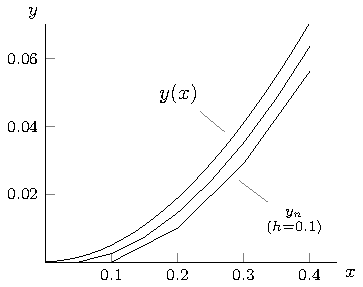
\includegraphics[]{figODEeuler}
\caption*{(ب)}
\end{subfigure}%
\caption{ترکیب یولر سے حاصل حل کا ریاضیاتی حل کے ساتھ موازنہ کیا گیا ہے۔}
\label{شکل_سادہ_اول_یولر_اصل_موازنہ}
\end{figure}

%====================
سوال \حوالہ{سوال_سادہ_اول_میدان_ڈھال_الف} تا سوال \حوالہ{سوال_سادہ_اول_میدان_ڈھال_ت} کے میدان ڈھال کو قلم و کاغذ سے کھینچتے ہوئے دیے ابتدائی نقطوں سے گزرتے منحنی حل حاصل کریں۔چند ڈھال میدان شکل \حوالہ{شکل_سوال_سادہ_اول_میدان_ڈھال_الف} اور شکل \حوالہ{شکل_سوال_سادہ_اول_میدان_ڈھال_پ} میں دیے گئے ہیں۔

%==========================

\حصہء{سوالات}
\ابتدا{سوال}\شناخت{سوال_سادہ_اول_میدان_ڈھال_الف}\quad \quad
$y'=1+y^2,\quad (\tfrac{\pi}{4},1)$
\انتہا{سوال}
%====================
\ابتدا{سوال}\شناخت{سوال_سادہ_اول_میدان_ڈھال_ب}\quad \quad
$y'=1-y^2,\quad (0,0)$
\انتہا{سوال}
%====================
\ابتدا{سوال}\شناخت{سوال_سادہ_اول_میدان_ڈھال_بب}\quad \quad
$yy'+8x=0,\quad (1,1)$
\انتہا{سوال}
%====================
\ابتدا{سوال}\شناخت{سوال_سادہ_اول_میدان_ڈھال_پ} \quad \quad
$y'=y-y^2,\quad (1,0)$
\انتہا{سوال}
%====================
\ابتدا{سوال} \شناخت{سوال_سادہ_اول_میدان_ڈھال_پپ}\quad \quad
$y'=x+\tfrac{1}{y},\quad (0,1)$
\انتہا{سوال}
%====================
\ابتدا{سوال} \شناخت{سوال_سادہ_اول_میدان_ڈھال_پپپ}\quad \quad
$y'=\sin^2 x,\quad (0,1)$
\انتہا{سوال}
%====================
\ابتدا{سوال}\شناخت{سوال_سادہ_اول_میدان_ڈھال_ت} \quad \quad
$y'=\sin^2 y,\quad (0,0)$
\انتہا{سوال}
%==================================
\begin{figure}
\centering
\begin{subfigure}{0.5\textwidth}
\centering
\begin{tikzpicture}
\def\length{sqrt(1+(1+y^2)^2)}
\begin{axis}[small, axis equal,axis lines*=middle,view={0}{90}, xlabel={$x$},ylabel={$y$},ylabel style={rotate=-90},ylabel style={at={(axis description cs:0.5,1.05)}},xmin=-4,xmax=4,ymin=-4,ymax=4,domain=-3.5:4, y domain=-3.5:4, samples=11,xlabel style={at={(axis description cs:1.05,0.5)}},xtick=\empty,ytick=\empty]
\addplot3 [gray, quiver={u={1/\length}, v={(1+y^2)/\length}, scale arrows=0.4,},-stealth] (x,y,0); %differential equation
\end{axis}
\end{tikzpicture}%
\caption*{(الف) \quad $y'=1+y^2$}
\end{subfigure}%
\begin{subfigure}{0.5\textwidth}
\centering
\begin{tikzpicture}
\def\length{sqrt(1+(1-y^2)^2)}
\begin{axis}[small, axis equal,axis lines*=middle,view={0}{90}, xlabel={$x$},ylabel={$y$},ylabel style={rotate=-90},ylabel style={at={(axis description cs:0.5,1.05)}},xmin=-4,xmax=4,ymin=-4,ymax=4,domain=-3.5:4, y domain=-3.5:4, samples=11,xlabel style={at={(axis description cs:1.05,0.5)}},xtick=\empty,ytick=\empty]
\addplot3 [gray, quiver={u={1/\length}, v={(1-y^2)/\length}, scale arrows=0.3},-stealth] (x,y,0); %differential equation
\end{axis}
\end{tikzpicture}%
\caption*{(ب) \quad $y'=1-y^2$}
\end{subfigure}%
\caption{سوال \حوالہ{سوال_سادہ_اول_میدان_ڈھال_الف} اور سوال \حوالہ{سوال_سادہ_اول_میدان_ڈھال_ب} کے ڈھال میدان۔}
\label{شکل_سوال_سادہ_اول_میدان_ڈھال_الف}
\end{figure}
%=============================
\begin{figure}
\centering
\begin{subfigure}{0.5\textwidth}
\centering
\begin{tikzpicture}
\def\length{sqrt(1+(-8*x/y)^2)}
\begin{axis}[small, axis equal,axis lines*=middle,view={0}{90}, xlabel={$x$},ylabel={$y$},ylabel style={rotate=-90},ylabel style={at={(axis description cs:0.5,1.05)}},xmin=-4,xmax=4,ymin=-4,ymax=4.5,domain=-3.8:4, y domain=-3.9:4, samples=11,xlabel style={at={(axis description cs:1.05,0.5)}},xtick=\empty,ytick=\empty]
\addplot3 [gray, quiver={u={1/\length}, v={(-8*x/y)/\length}, scale arrows=0.4,},-stealth] (x,y,0); %differential equation
\end{axis}
\end{tikzpicture}%
\caption*{(الف) \quad $y'=-\tfrac{8x}{y}$}
\end{subfigure}%
\begin{subfigure}{0.5\textwidth}
\centering
\begin{tikzpicture}
\def\length{sqrt(1+(y-y^2)^2)}
\begin{axis}[small, axis equal,axis lines*=middle,view={0}{90}, xlabel={$x$},ylabel={$y$},ylabel style={rotate=-90},ylabel style={at={(axis description cs:0.5,1.05)}},xmin=-4,xmax=4,ymin=-4,ymax=4,domain=-3.5:4, y domain=-3.5:4, samples=11,xlabel style={at={(axis description cs:1.05,0.5)}},xtick=\empty,ytick=\empty]
\addplot3 [gray, quiver={u={1/\length}, v={(y-y^2)/\length}, scale arrows=0.3},-stealth] (x,y,0); %differential equation
\end{axis}
\end{tikzpicture}%
\caption*{(ب) \quad $y'=y-y^2$}
\end{subfigure}%
\caption{سوال \حوالہ{سوال_سادہ_اول_میدان_ڈھال_بب} اور سوال \حوالہ{سوال_سادہ_اول_میدان_ڈھال_پ} کے ڈھال میدان۔}
\label{شکل_سوال_سادہ_اول_میدان_ڈھال_پ}
\end{figure}


%====================
ڈھال میدان کے استعمال سے تفرقی مساوات کے تمام حل سامنے آ جاتے ہیں۔بعض اوقات تفرقی مساوات کا تحلیلی حل حاصل کرنا ممکن ہی نہیں ہوتا۔درج ذیل دو سوالات میں ڈھال میدان سے اخذ حل اور دیے گئے تحلیلی حل کا موازنہ کرتے ہوئے ڈھال میدان سے حاصل حل کی درستگی کا اندازہ لگایا جا سکتا ہے۔

%=================
\ابتدا{سوال}\quad \quad
$y'=\sin x,\quad (\tfrac{\pi}{2},0),\quad y=-\cos x$
\انتہا{سوال}
%=====================
\ابتدا{سوال}\quad \quad
$y'=3x^2,\quad (0,0),\quad y=x^3$
\انتہا{سوال}
%=====================

%=============================
\ابتدا{سوال}
سوال \حوالہ{سوال_سادہ_اول_میدان_ڈھال_ب}، سوال \حوالہ{سوال_سادہ_اول_میدان_ڈھال_پ} اور سوال \حوالہ{سوال_سادہ_اول_میدان_ڈھال_ت} میں بے قابو متغیرہ \عددی{x} صریحاً  ظاہر نہیں کیا گیا ہے۔ایسی مساوات جن میں بے قابو متغیرہ کو صریحاً ظاہر نہ کیا جائے \اصطلاح{خود مختار}\فرہنگ{خود مختار!سادہ تفرقی مساوات}\فرہنگ{تفرقی!خود مختار}\حاشیہب{autonomous ordinary differential equations}\فرہنگ{autonomous!differential equation}\فرہنگ{differential!autonomous} سادہ تفرقی مساوات کہلاتے ہیں۔ خود مختار سادہ تفرقی مساوات کے  \اصطلاح{ہم میلان}\فرہنگ{ہم میلان}\حاشیہب{isoclines}\فرہنگ{isoclines} حل \عددی{f(x,y)=c} کی شکل و صورت کیا ہو گی؟

جواب:چونکہ \عددی{y'} کا دارومدار \عددی{x} پر نہیں ہے لہٰذا \عددی{x} تبدیل کرنے سے \عددی{y} کا میلان تبدیل نہیں ہو گا اور \عددی{f(x,y)=c} افقی محور کے متوازی خط ہوں گے۔ 
\انتہا{سوال}
%================

ایک جسم \عددی{y} محدد پر حرکت کرتی ہے۔لمحہ \عددی{t} پر نقطہ \عددی{y=0} سے جسم کا فاصلہ \عددی{y(t)} ہے۔سوالات \حوالہ{سوال_سادہ-اول_رفتار_الف} تا سوال \حوالہ{سوال_سادہ-اول_رفتار_پ} میں دئے شرائط کے مطابق جسم کی رفتار کی نمونہ کشی کریں۔ریاضی نمونے کی ڈھال میدان بناتے ہوئے  دیے گئے ابتدائی معلومات پر پورا اترتا منحنی خط کھینچیں۔ 

%=====================
\ابتدا{سوال}\شناخت{سوال_سادہ-اول_رفتار_الف}
جسم کی رفتار ضرب فاصلہ \عددی{y(t)} مستقل ہے جو \عددی{4} کے برابر ہے جبکہ \عددی{y(0)=4} کے برابر ہے۔

جوابات:\عددی{yy'=4}، \عددی{y=8t+16}
\انتہا{سوال}
%======================
\ابتدا{سوال}
رفتار ضرب وقت فاصلے کے برابر ہے۔لمحہ \عددی{t=1} پر فاصلہ \عددی{y(1)=2} ہے۔

جوابات:\عددی{y=y' t}، \عددی{y=2t}
\انتہا{سوال}
%=====================
\ابتدا{سوال}\شناخت{سوال_سادہ-اول_رفتار_پ}
مربع رفتار منفی مربع فاصلہ اکائی کے برابر ہے۔ابتدائی فاصلہ اکائی کے برابر ہے۔

جوابات:\عددی{y'=\sqrt{1+y^2}}، \عددی{\sinh^{-1}y=t+\sinh^{-1}1}
\انتہا{سوال}
%======================
\ابتدا{سوال}
ہوائی جہاز سے چھلانگ لگا کر زمین تک خیریت سے بذریعہ چھتری  اترا جا سکتا ہے۔گرتے ہوئے شخص پر آپس میں الٹ، دو عدد قوتیں عمل کرتی ہیں۔پہلی قوت زمینی کشش \عددی{F_1=mg} ہے جہاں \عددی{m} اس شخص کی کمیت اور \عددی{g=\SI{9.8}{\meter\per\second\squared}} ثقلی اسراع ہے۔یہ قوت انسان کو زمین کی طرف اسراع دیتی ہے۔دوسری قوت چھتری پر ہوا کے رگڑ سے پیدا قوت ہے جو اس شخص کی رفتار کو بڑھنے سے روکتی ہے۔چھتری پر ہوا کے رگڑ سے رفتار کے مربع کے متناسب قوت \عددی{F_2=cv^2} پیدا ہوتی ہے۔نیوٹن کی مساوات حرکت کہتی ہے کہ کسی بھی جسم پر قوت، اس جسم کی کمیت ضرب اسراع کے برابر ہوتی ہے۔چھتری سے زمین پر اترتے شخص کی نمونہ کشی کرتے ہوئے رفتار \عددی{v} کی سادہ تفرقی مساوات حاصل کریں۔کمیت کو \عددی{m=1} اور مستقل کو \عددی{c=1} لیتے ہوئے ڈھال میدان کھینچیں۔ تصور کریں کہ چھتری اس لمحہ کھلتی ہے جب شخص کی رفتار \عددی{v=\SI{15}{\meter\per\second}} ہو۔ایسی صورت میں منحنی حل حاصل کریں۔اس شخص کی اختتامی رفتار کیا ہو گی؟ کیا چھتری پر قوت رفتار کے راست متناسب ہونے کی صورت میں بھی چھتری کے ذریعہ ہوائی جہاز سے زمین تک خیریت سے چھلانگ لگائی جا سکتی ہے؟

جوابات:\عددی{mg-cv^2=m\tfrac{\dif v}{\dif t}}؛ گرنے کی رفتار اس قیمت پر رہتی ہے جہاں نیچے جانب قوت \عددی{mg} اور چھتری کی رکاوٹی اوپر جانب قوت \عددی{cv^2} برابر ہوں۔ایسی صورت میں گرتے شخص کی رفتار تبدیل نہیں ہوتی یعنی \عددی{y'=0} ہوتا ہے۔تفرقی مساوات میں \عددی{y'=0} پر کرتے اور \عددی{m=c=1} لیتے ہوئے اختتامی رفتار \عددی{v(t=\infty)=\SI{3.13}{\meter\per\second}} حاصل ہوتی ہے۔
\انتہا{سوال}
%=====================
\ابتدا{سوال}\شناخت{سوال_سادہ_اول_گول_دائرہ_ڈھال_میدان}
گول دائرے کی مساوات \عددی{x^2+y^2=r^2} ہے۔رداس \عددی{r} کو مستقل تصور کرتے ہوئے دائرے کی مساوات کا تفرق لیتے ہوئے  ڈھال میدان کی تفرقی مساوات حاصل کریں۔ڈھال میدان کھینچیں۔کیا آپ ڈھال میدان کو دیکھ کر کہہ سکتے ہیں کہ منحنی حل گول دائرے ہیں؟ اسی طرح \عددی{x^2+9y^2=c} کا تفرق لیتے ہوئے سادہ تفرقی مساوات حاصل کریں۔تفرقی مساوات کی ڈھال میدان کھینچیں۔ کیا ڈھال میدان کو دیکھ کر کہا جا سکتا ہے کہ منحنی حل بیضوی ہو گا؟

جوابات:\عددی{y'=-\tfrac{x}{y}}، \عددی{y'=-\tfrac{x}{9y}}
\begin{figure}
\centering
\begin{subfigure}{0.5\textwidth}
\centering
\begin{tikzpicture}
\def\length{sqrt(1+(x/y)^2)}
\begin{axis}[small, axis equal,axis lines*=middle,view={0}{90}, xlabel={$x$},ylabel={$y$},ylabel style={rotate=-90},ylabel style={at={(axis description cs:0.5,1.05)}},xmin=-4,xmax=4,ymin=-4,ymax=4,domain=-3.5:4, y domain=-3.5:4, samples=11,xlabel style={at={(axis description cs:1.05,0.5)}},xtick=\empty,ytick=\empty]
\addplot3 [gray, quiver={u={1/\length}, v={(-x/y)/\length}, scale arrows=0.3,},-stealth] (x,y,0); %differential equation
\end{axis}
\end{tikzpicture}%
\caption*{(الف) تفرقی مساوات \عددی{y'=-\tfrac{x}{y}} کی ڈھال میدان۔}
\end{subfigure}%
\begin{subfigure}{0.5\textwidth}
\centering
\begin{tikzpicture}
\def\length{sqrt(1+(x/(9*y))^2)}
\begin{axis}[small, axis equal,axis lines*=middle,view={0}{90}, xlabel={$x$},ylabel={$y$},ylabel style={rotate=-90},ylabel style={at={(axis description cs:0.5,1.05)}},xmin=-4,xmax=4,ymin=-4,ymax=4,domain=-3.5:4, y domain=-3.5:4, samples=11,xlabel style={at={(axis description cs:1.05,0.5)}},xtick=\empty,ytick=\empty]
\addplot3 [gray, quiver={u={1/\length}, v={(-x/(9*y))/\length}, scale arrows=0.3},-stealth] (x,y,0); %differential equation
\end{axis}
\end{tikzpicture}%
\caption*{(ب) تفرقی مساوات \عددی{y'=-\tfrac{x}{9y}} کی ڈھال میدان۔}
\end{subfigure}%
\caption{سوال \حوالہ{سوال_سادہ_اول_گول_دائرہ_ڈھال_میدان} کی ڈھال میدان۔}
\label{شکل_سوال_سادہ_اول_گول_دائرہ_ڈھال_میدان}
\end{figure}
\انتہا{سوال}
%===============================
سوال \حوالہ{سوال_سادہ_اول_یولر_الف} تا سوال \حوالہ{سوال_سادہ_اول_یولر_ت} کو ترکیب یولر سے حل کریں۔کل پانچ ہم فاصلہ نقطوں پر حل حاصل کریں۔ایک ہی کارتیسی محدد پر حاصل \عددی{y_1} تا \عددی{y_{5}} اور سوال میں دئے گئے حل \عددی{y(x)} کا خط کھینچیں۔
%=====================
\ابتدا{سوال}\شناخت{سوال_سادہ_اول_یولر_الف}
\begin{align*}
y'=-y,\quad y(0)=1,\quad h=0.1,\quad y(x)=e^{-x}
\end{align*}

جوابات: \عددی{y_1=0.9}، \عددی{y_2=0.81}، \عددی{y_3=0.729}، \عددی{y_4=0.6561}، \عددی{y_5=0.59049}
\انتہا{سوال}
%======================
\ابتدا{سوال}\شناخت{سوال_سادہ_اول_یولر_ب}
\begin{align*}
y'=-y,\quad y(0)=1,\quad h=0.01,\quad y(x)=e^{-x}
\end{align*}

جوابات: \عددی{y_1=0.99}، \عددی{y_2=0.9801}، \عددی{y_3=0.9703}، \عددی{y_4=0.9606}، \عددی{y_5=0.95099}
\انتہا{سوال}
%======================
\ابتدا{سوال}\شناخت{سوال_سادہ_اول_یولر_پ}
\begin{align*}
y'=1+3x^2,\quad y(1)=2,\quad h=0.1,\quad y(x)=x^3+x
\end{align*}

جوابات: \عددی{y_1=2.1}، \عددی{y_2=2.203}، \عددی{y_3=2.315}، \عددی{y_4=2.442}، \عددی{y_5=2.59}
\انتہا{سوال}
%======================
\ابتدا{سوال}\شناخت{سوال_سادہ_اول_یولر_ت}
\begin{align*}
y'=2xy,\quad y(0)=2,\quad h=0.01,\quad y(x)=e^{x^2-4}
\end{align*}

جوابات: \عددی{y_1=1.04}، \عددی{y_2=1.0818}، \عددی{y_3=1.1255}، \عددی{y_4=1.1712}، \عددی{y_5=1.2190}
\انتہا{سوال}
%======================

\حصہ{قابل علیحدگی سادہ تفرقی مساوات}
متعدد اہم سادہ تفرقی مساوات کو الجبرائی ترتیب دیتے ہوئے درج ذیل صورت میں لکھا جا سکتا ہے
\begin{align}\label{مساوات_سادہ_اول_قابل_علیحدگی-الف}
g(y)y'=f(x)
\end{align}
جس کو مزید یوں
\begin{align*}
g(y)\frac{\dif y}{\dif x} \dif x=f(x) \dif x
\end{align*}
یعنی
\begin{align*}
g(y)\dif y=f(x) \dif x
\end{align*}
لکھا جا سکتا ہے۔اس مساوات کے بائیں جانب صرف \عددی{y} متغیرہ اور دائیں جانب صرف \عددی{x} متغیرہ پایا جاتا ہے لہٰذا اس کا تکمل لیا جا سکتا ہے۔
\begin{align}\label{مساوات_سادہ_اول_قابل_علیحدگی-ب}
\int g(y)\dif y=\int f(x) \dif x+c
\end{align}
اگر \عددی{g(y)} اور \عددی{f(x)} قابل تکمل تفاعل ہوں تب مساوات \حوالہ{مساوات_سادہ_اول_قابل_علیحدگی-ب} سے مساوات \حوالہ{مساوات_سادہ_اول_قابل_علیحدگی-الف} کا حل حاصل کیا جا سکتا ہے۔اس ترکیب کو \اصطلاح{ترکیب علیحدگی متغیرات}\فرہنگ{ترکیب علیحدگی متغیرات}\فرہنگ{علیحدگی متغیرات!ترکیب}\حاشیہب{variable separation technique}\فرہنگ{variable separation} کہتے ہیں۔ مساوات \حوالہ{مساوات_سادہ_اول_قابل_علیحدگی-الف} کو \اصطلاح{قابل علیحدگی مساوات}\فرہنگ{قابل علیحدگی مساوات}\حاشیہب{separable equation}\فرہنگ{separable equation} کہتے ہیں۔

%=======================
\ابتدا{مثال}
مساوات \عددی{y'=1+y^2} قابل علیحدگی مساوات ہے چونکہ اس کو
\begin{align*}
\frac{\dif y}{1+y^2}=\dif x
\end{align*}
لکھا جا سکتا ہے جس کے دونوں اطراف کا تکمل لیتے ہوئے
\begin{align*}
\tan^{-1} y =x+c
\end{align*}
یعنی
\begin{align*}
y=\tan(x+c)
\end{align*}
حاصل ہوتا ہے جو تفرقی مساوات کا درکار حل ہے۔حاصل حل کو واپس تفرقی مساوات میں پر کرتے ہوئے تسلی کر لیں کہ یہی صحیح حل ہے۔
\انتہا{مثال}
%=================
\ابتدا{مثال}
قابل علیحدگی تفرقی مساوات \عددی{y'=xe^{-x} y^3} کو علیحدہ کرتے  ہوئے دونوں اطراف کا تکمل لے کر حل کرتے ہیں۔
\begin{align*}
y^{-3}\dif y&=xe^{-x} \dif x\\
\frac{y^{-2}}{-2}&=c-(x+1)e^{-x} \quad \quad \text{\RL{تکمل لیا گیا ہے}}\\
y^2&=\frac{1}{2(x+1)e^{-x}-2c}
\end{align*}
\انتہا{مثال}
%=================
\ابتدا{مثال}\شناخت{مثال_سادہ_اول_گھنٹی_الف}
درج ذیل ابتدائی قیمت تفرقی مساوات کو حل کریں۔
\begin{align*}
y'=-2xy,\quad y(0)=1
\end{align*} 

حل:مساوات کے متغیرات کو علیحدہ کرتے ہوئے تکمل کے ذریعہ حل کرتے ہیں۔
\begin{align*}
\int\frac{\dif y}{y}&=-\int 2x \dif x+c\\
\ln y&=-x^{2}+c_1\\
y&=ce^{-x^2}
\end{align*}
ابتدائی معلومات پر کرتے ہوئے \عددی{c=0} یعنی \عددی{c=e^{c_1}=1} ملتا ہے لہٰذا تفرقی مساوات کا مخصوص حل \عددی{y=e^{-x^2}} ہے جسے شکل \حوالہ{شکل_مثال_سادہ_اول_گھنٹی_الف} میں دکھایا گیا ہے اور جو \اصطلاح{گھنٹی نما}\فرہنگ{گھنٹی نما}\حاشیہب{bell shaped}\فرہنگ{bell shaped} ہے۔
\begin{figure}
\centering
\begin{tikzpicture}
\begin{axis}
\addplot[domain=-2:2,samples=60]{e^(-x^2)};
\end{axis}
\end{tikzpicture}
\caption{مثال \حوالہ{مثال_سادہ_اول_گھنٹی_الف} کا \اصطلاح{گھنٹی نما} حل۔}
\label{شکل_مثال_سادہ_اول_گھنٹی_الف}
\end{figure}
\انتہا{مثال}
%================
\ابتدا{مثال}\quad کاربن سے عمر دریافت کرنے کا طریقہ\\
طبعی معلومات: \اصطلاح{کائناتی شعاعیں}\فرہنگ{کائناتی شعاعیں}\حاشیہب{cosmic rays}\فرہنگ{cosmic rays} فضا میں تابکار کاربن \عددی{\ce{^{14}_{6}C}} بناتی ہیں۔یہ عمل زمین کی پیدائش سے اب تک ہوتا آ رہا ہے۔وقت کے ساتھ فضا میں \عددی{\ce{^{14}_{6}C}} اور \عددی{\ce{^{12}_{6}C}}\اصطلاح{ہم جا}\فرہنگ{ہم جا}\حاشیہب{isotopes}\فرہنگ{isotopes} کی تناسب ایک مخصوص قیمت حاصل کر چکی ہے۔کوئی بھی جاندار سانس لے کر یا خوراک کے ذریعہ فضا سے کاربن جذب  کرتا ہے۔یوں جب تک جانور زندہ رہے اس کی جسم میں دونوں ہم جا کاربن کی تناسب وہی ہو گی جو فضا میں ان کی تناسب ہے۔البتہ مرنے کے بعد جسم میں تابکار کاربن کی مقدار تابکاری تحلیل کی بنا گھٹتی ہے جبکہ غیر تابکار کاربن کی مقدار تبدیل نہیں ہوتی۔تابکار کاربن \عددی{\ce{^{14}_{6}C}} کی نصف زندگی \عددی{\num{5715}} سال ہے۔

اہرام مصر میں دفن مومیائی ہوئی فرعون کی لاش میں \عددی{\ce{^{14}_{6}C}} اور \عددی{\ce{^{12}_{6}C}} کا تناسب فضا کے تناسب کا \عددی{\SI{56.95}{\percent}} ہے۔لاش کی عمر دریافت کریں۔

حل:تابکار کاربن کی نصف زندگی سے تابکاری تحلیل کا مستقل \عددی{k} دریافت کرتے ہیں۔
\begin{align*}
y_0e^{-k(5715)}=\frac{y_0}{2}, \quad e^{-k(5715)}=\frac{1}{2}, \quad -k=\frac{\ln (\frac{1}{2})}{5715}, \quad k=0.0001213
\end{align*}
لاش میں ہم جا کاربن کی تناسب سے لاش کی عمر حاصل کرتے ہیں۔
\begin{align*}
e^{-0.0001213t}=0.5695,\quad -0.0001213t=\ln 0.5695,\quad t=4641
\end{align*}
یوں فرعون کی لاش \عددی{\num{4641}} سال پرانی ہے۔

\انتہا{مثال}
%=================
\ابتدا{مثال}\شناخت{مثال_سادہ_اول_مرکب}\quad مرکب بنانے کا عمل\\
کیمیائی صنعت میں  مرکب بنانے کا عمل عام ہے۔شکل \حوالہ{شکل_مثال_سادہ_اول_مرکب}-الف میں  پانی کی ٹینکی دکھائی گئی ہے جس میں ابتدائی طور پر \عددی{1000} لٹر پانی پایا جاتا ہے۔اس پانی میں کل \عددی{\SI{100}{\kilo\gram}} نمک ملایا گیا ہے۔پانی کو مسلسل ہلانے سے ٹینکی میں کثافت یکساں رکھی جاتی ہے۔ٹینکی میں \عددی{40} لٹر فی منٹ کی شرح سے نمکین پانی شامل کیا جاتا ہے۔اس پانی میں نمک کی مقدار \عددی{\SI{0.5}{\kilo\gram\per\litre}} ہے۔ٹینکی سے نمکین پانی کا انخلا \عددی{40} لٹر فی منٹ ہے۔ٹینکی میں نمک کی کل مقدار بالمقابل وقت دریافت کریں۔
\begin{figure}
\centering
\begin{subfigure}{0.5\textwidth}
\centering
\begin{tikzpicture}
   [ragged border/.style={ decoration={random steps, segment length=1mm, amplitude=0.5mm},
           decorate,}]
\pgfmathsetmacro{\x}{2}
\pgfmathsetmacro{\y}{2}

\fill[cyan!30]
        decorate[ragged border]{
        (-\x-\x/4,\y/2)--++(\x,0)
        }
        -- ++(0,-3/8*\y) --++ (\x/4,0) --++ (0,-\y/8) --++ (-\x-\x/4,0) --++(0,\y/2) -- cycle;
\fill[cyan!30](-\x-\x/4,3/4*\y)coordinate(inL)--++(-\x/4,0)--++(0,\y/8)--++(\x/4,0)coordinate(inU)--cycle;
\fill[cyan!30] (inL) to [out=0,in=120] ++(\x/4,-\y/3)--++(\x/16,0) to [out=120,in=0] (inU)--cycle;

\draw(0,0)--++(-\x-\x/4,0)--++(0,3/4*\y)--++(-\x/4,0)++(0,\y/8)--++(\x/4,0)--++(0,\y/4);
\draw(0,\y/8)--++(-\x/4,0)--++(0,\y);
\draw[cyan!30,-stealth,ultra thick] (\x/8,\y/16)--++(\x/4,0)node[right,color=black]{خروج};
\draw[cyan!30,stealth-,ultra thick] (-\x-\x/4-\x/4-\x/8,3/4*\y+\y/16)--++(-\x/4,0)node[pos=0.5,above,color=black]{دخول};
\end{tikzpicture}
\caption*{(الف)}
\end{subfigure}%
\begin{subfigure}{0.5\textwidth}
\centering
\begin{tikzpicture}
\begin{axis}[small,xlabel={$t\, (\text{\RL{منٹ}})$}, ylabel={$y(t)$},ylabel style={rotate=-90},ylabel style={at={(axis description cs:0,1.05)}}]
\addplot[domain=0:150]{500-400*e^(-0.04*x)};
\end{axis}
\end{tikzpicture}
\caption*{(ب)}
\end{subfigure}%
\caption{مثال \حوالہ{مثال_سادہ_اول_مرکب} میں مرکب بنانے کا عمل۔}
\label{شکل_مثال_سادہ_اول_مرکب}
\end{figure}

حل:چونکہ ٹینکی میں پانی شامل ہونے کی شرح اور پانی خارج ہونے کی شرح  برابر ہےیں لہٰذا ٹینکی میں پانی کی مقدار تبدیل نہیں ہوتی۔ٹینکی میں داخل ہونے والا ایک لٹر کا نمکین پانی \عددی{\SI{0.5}{\kilo\gram}} نمک ٹینکی میں شامل کرتا ہے۔یوں \عددی{40} لٹر فی منٹ سے داخل ہوتا پانی \عددی{40\times 0.5=\SI{20}{\kilo\gram\per\minute}} سے نمک شامل کرتا ہے۔کسی بھی لمحہ ٹینکی میں کل نمک کو \عددی{y} کلوگرام لکھتے ہوئے ٹینکی میں نمک کی کثافت کو \عددی{\tfrac{y}{1000}} کلوگرام فی لٹر لکھا جا سکتا ہے۔یوں خارج ہوتا پانی \عددی{40\times \tfrac{y}{1000}} کلوگرام فی منٹ نمک خارج کرتا ہے۔اس طرح نمک میں اضافے کی شرح \عددی{\tfrac{\dif y}{\dif t}} کو
\begin{align*}
y'&=\text{\RL{نمک شامل ہونے کی شرح}} -\text{\RL{نمک خارج ہونے کی شرح}}\quad \quad (\text{\RL{متوازن مساوات}})\\
&=20-\frac{40y}{1000}
\end{align*}
یعنی
\begin{align}
y'=0.04(500-y)
\end{align}
لکھا جا سکتا ہے جو قابل علیحدگی مساوات ہے لہٰذا اس میں متغیرات کو علیحدہ کرتے ہوئے تکمل کے ذریعہ حل کرتے ہیں۔
\begin{align*}
\frac{\dif y}{y-500}=-0.04\dif t, \quad \ln \abs{y-500}=-0.04t+c_1,\quad y=500+ce^{-0.04t}
\end{align*}
ٹینکی میں ابتدائی نمک کی کل مقدار \عددی{\SI{100}{\kilo\gram}} ہے۔اس معلومات کو درج بالا میں پر کرتے ہوئے مساوات کا مستقل \عددی{c} حاصل کرتے ہیں۔ 
\begin{align*}
100=500+c^{-0.04(0)},\quad c=-400
\end{align*}
یوں کسی بھی لمحے ٹینکی میں کل نمک کی مقدار درج ذیل ہے جس کو شکل-ب میں دکھایا گیا ہے۔
\begin{align*}
y(t)=500-400e^{-0.04t}
\end{align*}
شکل-ب کے مطابق ٹینکی میں آخرکار کل \عددی{\SI{500}{\kilo\gram}} نمک پایا جائے گا۔ یہی جواب بغیر کسی مساوات لکھے بھی حاصل کیا جا سکتا ہے۔اگر ٹینکی میں لگاتار نمکین پانی شامل کیا جائے اور اس سے پرانا پانی خارج کیا جائے تو آخرکار ٹینکی میں صرف نیا شامل کردہ پانی ہی پایا جائے گا۔چونکہ شامل کردہ پانی میں \عددی{0.5} کلوگرام فی لٹر نمک پایا جاتا ہے لہٰذا \عددی{1000} لٹر کی ٹینکی میں کل نمک \عددی{1000\times 0.5=\SI{500}{\kilo\gram}} ہو گا۔ 
\انتہا{مثال}
%=====================
\ابتدا{مثال}\شناخت{مثال_سادہ_اول_نیوٹن_قانون_ٹھنڈک} \quad نیوٹن قانون ٹھنڈک
گرمیوں میں ایک دفتر کا درجہ حرارت ایئر کنڈشنر کی مدد سے \عددی{\SI{21}{\degree\celsius}} پر رکھا جاتا ہے۔صبح سات بجے ایئر کنڈشنر چالو کیا جاتا ہے اور شام نو بجے اس کو بند کر دیا جاتا ہے۔ایک مخصوص دن کو شام نو بجے بیرونی درجہ حرارت \عددی{\SI{40}{\degree\celsius}} ہوتا ہے جبکہ صبح سات بجے بیرونی درجہ حرارت \عددی{\SI{30}{\degree\celsius}} تک گر چکا ہوتا ہے۔دفتر کے اندر رات دو بجے درجہ حرارت \عددی{\SI{26}{\degree\celsius}} ہوتا ہے۔صبح سات بجے دفتر کے اندر درجہ حرارت معلوم کریں۔

طبعی معلومات:تجربے سے معلوم کیا گیا ہے کہ حرارتی توانائی کو با آسانی منتقل کرتے جسم (مثلاً لوہا) کے درجہ حرارت میں تبدیلی کی شرح جسم اور اس کے گرد ماحول کے درجہ حرارت میں فرق کے راست تناسب  ہوتا ہے۔اس کو \اصطلاح{نیوٹن کا قانون ٹھنڈک}\فرہنگ{نیوٹن کا قانون ٹھنڈک}\حاشیہب{Newton's law of cooling}\فرہنگ{Newton!law of cooling} کہا جاتا ہے۔

حل:پہلا قدم: نمونہ کشی \\
دفتر کے اندرونی حرارت کو \عددی{T} سے ظاہر کرتے ہیں جبکہ بیرونی حرارت کو \عددی{T_b} سے ظاہر کرتے ہیں۔یوں نیوٹن کا قانون ٹھنڈک کی ریاضیاتی صورت درج ذیل ہو گی۔
\begin{align}
\frac{\dif T}{\dif t}=k(T-T_b)
\end{align}
دوسرا قدم:عمومی حل کی تلاش\\
اگرچہ دفتر کی دیواریں اور چھت حرارتی توانائی با آسانی منتقل نہیں کرتی ہم اسی کلیے کا سہارا لیتے ہوئے مسئلہ حل کریں گے۔یہاں بیرونی درجہ حرارت مستقل قیمت نہیں ہے لہٰذا درج بالا مساوات کو حل کرنا مشکل ہو گا۔انجنیئرنگ کے شعبے میں عموماً ایسی ہی مشکلات کا سامنہ کرنا ہوتا ہے۔ہمیں مسئلے کی سادہ صورت حل کرنا ہو گی۔اگر ہم تصور کریں کہ \عددی{T_b} مستقل قیمت ہے تب درج بالا مساوات کے متغیرات علیحدہ کئے جا سکتے ہیں۔چونکہ بیرونی درجہ حرارت \عددی{\SI{30}{\degree\celsius}} تا \عددی{\SI{40}{\degree\celsius}} رہا ہے لہٰذا ہم اس کی اوسط قیمت یعنی \عددی{\SI{35}{\degree\celsius}} کو بیرونی درجہ حرارت تصور کرتے ہوئے مسئلے کو حل کرتے ہیں۔مساوات کے متغیرات علیحدہ کرتے ہوئے تکمل لے کر اس کو حل کرتے ہیں۔
\begin{align*}
\frac{\dif T}{T-35}=k\dif t, \quad \ln\abs{T-35}=kt+c_1,\quad T-35=ce^{kt}
\end{align*}
تیسرا قدم:مخصوص حل کا حصول\\
اگر شام نو بجے کو لمحہ \عددی{t=0} لیا جائے اور وقت کو گھنٹوں میں ناپا جائے تب \عددی{T(0)=21} لکھا جائے گا جسے درج بالا میں پر کرتے ہوئے \عددی{c=-14} حاصل ہوتا ہے۔یوں مخصوص حل
\begin{align*}
T=35-14e^{kt}
\end{align*}
چوتھا قدم:مستقل \عددی{k} کا حصول\\
ہم جانتے ہیں کہ رات دو بجے  اندرونی درجہ حرارت  \عددی{\SI{26}{\degree\celsius}} ہے۔یاد رہے کہ شام نو بجے کو لمحہ \عددی{t=0} لیا گیا لہٰذا رات دو بجے \عددی{t=5} ہو گا۔
یوں \عددی{T(5)=26} لکھا جائے گا۔ان معلومات کو درج بالا مساوات میں پر کرتے ہوئے \عددی{k} حاصل کرتے ہوئے مکمل مساوات حاصل کرتے ہیں۔
\begin{align*}
26=35-14e^{5k},\quad k=-0.088, \quad T=35-14e^{-0.088t}
\end{align*}
آخری قدم:\\
صبح سات بجے اندرونی درجہ حرارت کا تخمینہ لگاتے ہیں یعنی \عددی{t=10} پر درجہ حرارت درکار ہے۔
\begin{align*}
T=35-14e^{-0.088(10)}=\SI{29.2}{\degree\celsius}
\end{align*} 
پوری رات میں اندرونی درجہ حرارت \عددی{\SI{8.2}{\degree\celsius}} بڑھ گیا ہے۔شکل \حوالہ{شکل_مثال_سادہ_اول_نیوٹن_قانون_ٹھنڈک} میں اندرونی درجہ حرارت بالمقابل وقت دکھایا گیا ہے۔
\begin{figure}
\centering
\begin{tikzpicture}
\begin{axis}[small,xlabel={$t\,\text{(گھنٹے)}$},ylabel={$T\, (\si{\degree\celsius})$},ytick={21,29.2},yticklabels={$21$,$29.2$},ylabel style={rotate=-90},ylabel style ={at={(axis description cs:0,1.05)}},xmin=0]
\addplot[domain=0:10]{35-14*e^(-0.088*x)};
\end{axis}
\end{tikzpicture}
\caption{مثال \حوالہ{مثال_سادہ_اول_نیوٹن_قانون_ٹھنڈک}: دفتر کا اندرونی درجہ حرارت بالمقابل وقت۔}
\label{شکل_مثال_سادہ_اول_نیوٹن_قانون_ٹھنڈک}
\end{figure}
\انتہا{مثال}
%=======================
\ابتدا{مثال} \quad پانی کا انخلا:\شناخت{مثال_سادہ_اول_ٹاری_سلی}
پانی کی ٹینکی کا رقبہ عمودی تراش \عددی{B=\SI{2}{\meter\squared}} ہے۔ٹینکی کی تہہ میں \عددی{r=\SI{0.5}{\centi\meter}} رداس کا گول سوراخ ہے جس سے پانی نکل رہا ہے۔ٹینکی میں پانی کی ابتدائی گہرائی \عددی{h_1=\SI{1.5}{\meter}} ہے۔ٹینکی کتنی دیر میں خالی ہو گی۔

طبعی معلومات:پانی کی سطح پر \عددی{m} کمیت پانی کی مخفی توانائی \عددی{mgh} ہے جہاں \عددی{g=\SI{9.8}{\meter\per\second\squared}} ثقلی اسراع اور \عددی{h} پانی کی گہرائی ہے۔سوراخ سے خارج ہوتے وقت یہ مخفی توانائی  حرکی توانائی \عددی{\tfrac{mv^2}{2}} میں تبدیل ہو جاتی ہے جہاں \عددی{v} رفتار کو ظاہر کرتی ہے۔مخفی توانائی اور حرکی توانائی کو برابر لکھتے ہوئے \عددی{v} کے لئے حل کرتے ہیں۔
\begin{align*}
\frac{mv^2}{2}=mgh,\quad v=\sqrt{2gh}
\end{align*}
شکل \حوالہ{شکل_مثال_سادہ_اول_ٹاری_سلی}-الف میں پانی کی دھار دکھائی گئی ہے۔جیسا کہ آپ دیکھ سکتے ہیں دھار سوراخ کے قریب سکڑتا ہے۔اگر سوراخ کا رقبہ \عددی{a} ہو تب سکڑے  ہوئے مقام پر دھار کا رقبہ عمودی تراش \عددی{0.6a} ہوتا ہے۔یوں سوراخ سے نکلا تمام پانی رقبہ \عددی{0.6a} سے گزرتا ہے اور یہی وہ مقام ہے جہاں پانی کا ہر ذرہ ایک ہی سمت میں رفتار \عددی{v} سے حرکت کرتا ہے۔

شکل \حوالہ{شکل_مثال_سادہ_اول_ٹاری_سلی}-ب میں ایک نالی دکھائی گئی ہے جس میں پانی کی رفتار \عددی{v} ہے۔ نالی کا رقبہ عمودی تراش \عددی{A} ہے۔لمحہ \عددی{t=0} پر  مقام \عددی{m} پر موجود پانی کا ذرہ وقت \عددی{\Delta t} میں \عددی{v\Delta} فاصلہ طے کرتے ہوئے مقام \عددی{n} تک پہنچ جائے گا۔یوں \عددی{\Delta t} کے دوران مقام \عددی{m} سے گزرا ہوا پانی نالی کو \عددی{m} تا \عددی{n} بھرے گا۔اس پانی کی مقدار \عددی{\Delta M=A v \Delta t} ہو گی۔اسی کلیے کو استعمال کرتے ہوئے شکل \حوالہ{شکل_مثال_سادہ_اول_ٹاری_سلی}-الف میں \عددی{\dif t} دورانیے میں کل \عددی{\dif M=0.6a v \dif t} پانی خارج ہو گا۔یوں پانی کی شرح انخلا درج ذیل ہو گی۔
 \begin{align}\label{مساوات_سادہ_اول_ٹورا_سلی}
\frac{\dif M}{\dif t}=0.6a\sqrt{2gh}
\end{align}
 
اس مساوات  کو \اصطلاح{قانون ٹاری سلی}\فرہنگ{قانون ٹاری سلی}\حاشیہب{Torricelli's law}\فرہنگ{Torricelli's law} کہتے ہیں۔
\begin{figure}
\centering
\begin{subfigure}{0.5\textwidth}
\centering
\begin{tikzpicture}
  [ragged border/.style={ decoration={random steps, segment length=1mm, amplitude=0.5mm},
           decorate,}]
\pgfmathsetmacro{\x}{2}
\pgfmathsetmacro{\y}{2}
\pgfmathsetmacro{\angA}{70}
\pgfmathsetmacro{\angB}{110}
%coloured water
\path(-\x/2-\x/16,0) to [out=-\angA,in=\angA]++(0,-\y/4)coordinate(kL);
\path(-\x/2+\x/16,0) to [out=-\angB,in=\angB]++(0,-\y/4)coordinate(kR);
\fill[cyan!30](-\x,\y-\y/8)--++(\x,0)-- ++(0,-\y+\y/8) --++ (-\x,0) --++ (0,\y-\y/8) -- cycle;
\fill[cyan!30] (-\x/2-\x/16,0) to [out=-\angA,in=\angA] (kL)--(kR) to [out=\angB,in=-\angB] ++(0,\y/4)--cycle;
\draw[stealth-stealth] (\x/8,0)--++(0,\y-\y/8)node[pos=0.5,fill=white]{$h$};
%drum
\draw(0,0)--++(0,\y);
\draw(0,0)--++(-\x/2+\x/16,0)++(-\x/8,0)--++(-\x/2+\x/16,0)--++(0,\y);
\draw[stealth-](-\x/2-\x/16,-\y/8)--++(-\x/4,0)--++(-\x/8,-\y/8)node[left]{$0.6a$};
\draw (-\x-\x/16,\y-\y/8)--++(-\x/4,0);
\draw (-\x-\x/16,\y-\y/8-\y/16)--++(-\x/4,0);
\draw[stealth-](-\x-\x/16-\x/8,\y-\y/8)--++(0,\y/4)node[above]{$\dif h$};
\draw[stealth-](-\x-\x/16-\x/8,\y-\y/8-\y/16)--++(0,-\y/4);
\end{tikzpicture}
\caption*{(الف)}
\end{subfigure}%
\begin{subfigure}{0.5\textwidth}
\centering
\begin{tikzpicture}
\pgfmathsetmacro{\x}{2}
\pgfmathsetmacro{\y}{2}
%water
\fill[cyan!10](0,0)--++(2*\x,0)--++(0,\y/8)--++(-2*\x,0)--cycle;
\fill[cyan!30](\x/2,0)--++(\x,0)--++(0,\y/8)--++(-\x,0)--cycle;
\draw[stealth-](-\x/8,\y/16)--++(-\x/4,0)node[pos=0.5,above]{$v$};
\draw[stealth-stealth](\x/2,-\y/8)--++(\x,0)node[pos=0.5,fill=white]{$v \Delta t$};
\draw(\x/2+\x/2,\y/16)--++(\x/2,\y/2)node[right]{$\Delta M=A v\Delta t$};
%pipe
\draw(0,\y/8)--++(2*\x,0);
\draw(0,0)--++(2*\x,0);
\draw[stealth-](\x/4,\y/8)--++(0,\y/4)--++(-\x/4,\y/4)node[above]{\RL{رقبہ عمودی تراش=$A$}};
\draw[dashed] (\x/2,-\y/4)node[below]{$m$}--++(0,\y/2);
\draw[dashed] (\x+\x/2,-\y/4)node[below]{$n$}--++(0,\y/2);

\end{tikzpicture}
\caption*{(ب)}
\end{subfigure}%
\caption{مثال \حوالہ{مثال_سادہ_اول_ٹاری_سلی}: پانی کا انخلا اور پانی کے دھار کا سکڑنا۔}
\label{شکل_مثال_سادہ_اول_ٹاری_سلی}
\end{figure}

حل:دورانیہ \عددی{\dif t} میں پانی کی انخلا کے بنا ٹینکی میں پانی کی گہرائی \عددی{\dif h} کم ہو گی جو \عددی{B \dif h} حجم کی کمی کو ظاہر کرتی ہے جہاں \عددی{B} ٹینکی کا رقبہ عمودی تراش ہے۔چونکہ پانی کے انخلا سے ٹینکی میں پانی کم ہوتا ہے لہٰذا درج ذیل لکھا جا سکتا ہے جو دیے گئے مسئلے کا تفرقی مساوات ہے۔
\begin{align}
0.6a\sqrt{2gh} \dif t=-B\dif h
\end{align}
متغیرات کو علیحدہ کرتے ہوئے حل کرتے ہیں۔
\begin{align*}
\frac{\dif h}{\sqrt{h}}=-\frac{0.6a \sqrt{2g}}{B} \dif t,\quad 2\sqrt{h}=-\frac{0.6a \sqrt{2g}}{B} t+c
\end{align*}
ابتدائی لمحہ \عددی{t=0} پر پانی کی گہرائی \عددی{h_1} ہے۔ان معلومات کو درج بالا میں پر کرتے ہوئے \عددی{c=2h_1} ملتا ہے لہٰذا تفرقی مساوات کا مخصوص حل درج ذیل ہے۔
\begin{align}\label{مساوات_سادہ_اول_ٹاری_سلی_ٹینکی_خالی}
 2\sqrt{h}=-\frac{0.6a \sqrt{2g}}{B} t+ 2\sqrt{h_1}
\end{align}
خالی ٹینکی سے مراد \عددی{h=0} ہے۔مخصوص حل میں \عددی{h=0} پر کرتے ہوئے ٹینکی خالی کرنے کے لئے درکار وقت حاصل کرتے ہیں۔
\begin{align*}
 2\sqrt{0}=-\frac{0.6a \sqrt{2g}}{B} t+ 2\sqrt{h_1}, \quad t=\frac{2\sqrt{h_1} B}{0.6a \sqrt{2g}}\\
t=\frac{2\sqrt{1.5} \times 2}{0.6\pi 0.005^2 \sqrt{2\times 9.8}}=\SI{23482}{\second} \approx \SI{6.52}{\hour}
\end{align*}
مساوات \حوالہ{مساوات_سادہ_اول_ٹاری_سلی_ٹینکی_خالی} کو شکل \حوالہ{شکل_مثال_سادہ_اول_ٹاری_سلی_خالی} میں دکھایا گیا ہے۔یاد رہے کہ \عددی{\SI{23482}{\second}} میں ٹینکی خالی ہو جاتی ہے لہٰذا ترسیم کو اتنے وقت کے لئے ہی کھینچا گیا ہے۔
\begin{figure}
\centering
\begin{tikzpicture}
\begin{axis}[axis lines*=middle,ylabel={$h$},ylabel style={rotate=-90},ylabel style={at={(axis description cs:0,1.05)}},xlabel={$t\, (\si{\second})$},scaled x ticks=false]
\pgfmathsetmacro{\ha}{1.5}
\pgfmathsetmacro{\B}{2}
\pgfmathsetmacro{\a}{pi*0.005^2}
%\pgfmathsetmacro{\k}{0.3*\a*sqrt(2*9.8)/\B}  %pgfmath calculate this value wrongly????
\pgfmathsetmacro{\k}{0.000052}
%
\addplot[domain=0:23480]({x},{(sqrt(\ha)-\k*x)^(2)});
\end{axis}
\end{tikzpicture}
\caption{مثال \حوالہ{مثال_سادہ_اول_ٹاری_سلی}: ٹینکی خالی ہونے کا عمل۔}
\label{شکل_مثال_سادہ_اول_ٹاری_سلی_خالی}
\end{figure}
\انتہا{مثال}
%======================

\جزوحصہء{علیحدگی متغیرات کی جامع ترکیب}
بعض اوقات نا قابل علیحدگی تفرقی مساوات کے متغیرات کو تبدیل کرتے ہوئے مساوات کو قابل علیحدگی بنایا جا سکتا ہے۔ اس ترکیب کو درج ذیل عملاً اہم قسم کی مساوات کے لئے سیکھتے ہیں جہاں \عددی{f(\tfrac{y}{x})} قابل تفرق تفاعل ہے مثلاً \عددی{\cos \tfrac{y}{x}}، \عددی{e^{(y/x)}} وغیرہ۔
\begin{align}
y'=f\left(\frac{y}{x}\right)
\end{align}  
مساوات کی صورت دیکھتے ہوئے \عددیء{\tfrac{y}{x}=u} لیتے ہیں۔یوں درج ذیل لکھا جا سکتا ہے
\begin{align}\label{مساوات_سادہ_اول_جامع_علیحدگی_الف}
y=ux,\quad y'=u+xu'
\end{align}
جنہیں \عددی{y'=f(\tfrac{y}{x})} میں پر کرتے ہوئے \عددی{u+xu'=f(u)} یعنی \عددی{xu'=f(u)-u} ملتا ہے۔اگر \عددی{f(u)-u \ne 0} ہو تب متغیرات علیحدہ کرتے ہوئے درج ذیل لکھا جا سکتا ہے۔
\begin{align} 
\frac{\dif u}{f(u)-u}=\frac{\dif x}{x}
\end{align}
%============
\ابتدا{مثال}
تفاعل \عددی{xy'-y=2x} کو حل کریں۔

حل:تفاعل کو \عددی{y'=\tfrac{y}{x}+2} لکھا جا سکتا ہے۔یوں \عددی{\tfrac{y}{x}=u} لیتے ہوئے  مساوات \حوالہ{مساوات_سادہ_اول_جامع_علیحدگی_الف} کے استعمال سے درج ذیل ملتا ہے۔
\begin{align*}
u+xu'=u+2, \quad \dif u=2\frac{\dif x}{x},\quad u=2\ln \abs{x}+c
\end{align*}
اس میں \عددی{u} کی جگہ واپس \عددی{\tfrac{y}{x}} پر کرتے ہوئے جواب حاصل ہوتا ہے۔
\begin{align*}
\frac{y}{x}=2\ln \abs{x}+c,\quad y=2x\ln \abs{x}+cx
\end{align*}
\انتہا{مثال}
%=========================

\حصہء{سوالات}
سوال \حوالہ{سوال_سادہ_اول_جامع_علیحدگی_الف} تا سوال \حوالہ{سوال_سادہ_اول_جامع_علیحدگی_ب} کے عمومی حل حاصل کریں۔حاصل حل کو واپس تفرقی مساوات میں پر کرتے ہوئے اس کی درستگی ثابت کریں۔

%=======================
\ابتدا{سوال}\شناخت{سوال_سادہ_اول_جامع_علیحدگی_الف}
$y^2y'+x^2=0$

جواب:\عددی{x^3+y^3=c}
\انتہا{سوال}
%=============================
\ابتدا{سوال}
$yy'+x=0$

جواب:\عددی{x^2+y^2=c}
\انتہا{سوال}
%=============================
\ابتدا{سوال}
$y'=\sec^2 y$

جواب:\عددی{y=\tan x+c}
\انتہا{سوال}
%=============================
\ابتدا{سوال}
$y'\cos x=y\sin x$

جواب:\عددی{y=c\sec x}
\انتہا{سوال}
%=============================
\ابتدا{سوال}
$y'=ye^{x-1}$

جواب:\عددی{\ln\abs{y}=e^{x-1}+c}
\انتہا{سوال}
%=============================
\ابتدا{سوال} 
\عددی{u=\tfrac{y}{x}} پر کرتے ہوئے \عددی{xy'=y+x^2\sin^2\frac{y}{x}} کو حل کریں۔

جواب:\عددی{\tfrac{\cos \tfrac{y}{x}-1}{\cos\tfrac{y}{x}+1}=ce^{2x}}
\انتہا{سوال}
%=============================
\ابتدا{سوال}
\عددی{y'=(2x+y)^2} کو حل کریں۔ایسا کرنے کی خاطر \عددی{u=2x+y} پر کرنا ہو گا۔

جواب:\عددی{y=-2x+\sqrt{2}\tan(\sqrt{2}x+c)}
\انتہا{سوال}
%=============================
\ابتدا{سوال} 
\عددی{u=\tfrac{y}{x}} پر کرتے ہوئے \عددی{xy'=y^2+y} کو حل کریں۔

جواب:\عددی{y=-\tfrac{x}{x+c}}
\انتہا{سوال}
%=============================
\ابتدا{سوال} \شناخت{سوال_سادہ_اول_جامع_علیحدگی_ب}
\عددی{u=\tfrac{y}{x}} پر کرتے ہوئے \عددی{xy'=x-y} کو حل کریں۔

جواب:\عددی{xy-x^2=c}
\انتہا{سوال}
%=============================

 ابتدائی قیمت سوال \حوالہ{سوال_سادہ_اول_ابتدائی_قیمت_الف} تا سوال \حوالہ{سوال_سادہ_اول_ابتدائی_قیمت_ب} کے مخصوص حل حاصل کریں۔

\ابتدا{سوال}\شناخت{سوال_سادہ_اول_ابتدائی_قیمت_الف}
\begin{align*}
xy'+y=0,\quad y(2)=8
\end{align*}

جواب:\عددی{y=\tfrac{16}{x}}
\انتہا{سوال}
%====================
\ابتدا{سوال}
\begin{align*}
y'=1+9y^2,\quad y(1)=0
\end{align*}

جواب:\عددی{y=\tfrac{1}{3}\tan[3(x-1)]}
\انتہا{سوال}
%======================
\ابتدا{سوال}
\begin{align*}
y' \cos^2 x=\sin^2 y, \quad y(0)=\frac{\pi}{4}
\end{align*}

جواب:\عددی{\tan y=\tfrac{1}{1-\tan x}}
\انتہا{سوال}
%==============================
\ابتدا{سوال}
\begin{align*}
y'=-4xy,\quad y(0)=5
\end{align*}

جواب:\عددیء{y=5e^{-2x^2}}
\انتہا{سوال}
%==================
\ابتدا{سوال}
\begin{align*}
y'=-\frac{2x}{y},\quad y(1)=2
\end{align*}

جواب:\عددی{2x^2+y^2=6}
\انتہا{سوال}
%==================
\ابتدا{سوال}
\begin{align*}
y'=(x+y-4)^2,\quad y(0)=5
\end{align*}

جواب:\عددی{x+y-4=\tan(x+\tfrac{\pi}{4})}
\انتہا{سوال}
%=================
\ابتدا{سوال}\شناخت{سوال_سادہ_اول_ابتدائی_قیمت_ب}
\begin{align*}
xy'=y+3x^4\cos^2 \frac{y}{x},\quad y(1)=0
\end{align*}

 جواب:اس میں \عددی{u=\tfrac{y}{x}} پر کرنے سے \عددی{\tan \tfrac{y}{x}=x^3-1} ملتا ہے۔
\انتہا{سوال}
%=================
\ابتدا{سوال}
کسی بھی لمحے پر جرثوموں کی تعداد بڑھنے کی شرح، اس لمحے موجود جرثوموں کی تعداد کے راست تناسب ہے۔اگر ان کی تعداد دو گھنٹوں میں دگنی ہو جائے تب چار گھنٹوں بعد ان کی تعداد کتنی ہو گی؟ چوبیس گھنٹوں بعد کتنی ہو گی؟  

جوابات:\عددی{y=y_0e^{0.34657t}}، \عددی{4y_0}، \عددی{4095y_0}
\انتہا{سوال}
%==================
\ابتدا{سوال}
جرثوموں کی شرح پیدائش موجودہ تعداد کے راست تناسب ہے۔ان کی شرح اموات بھی موجودہ تعداد کے راست تناسب ہے۔جرثوموں کی تعداد بڑھنے کی شرح کیا ہو گی؟ تعداد بالمقابل وقت کیا ہو گا؟ تعداد کہاں متوازن صورت اختیار کرے گی؟

جوابات:\عددی{\tfrac{\dif y}{\dif t}=\alpha y-\beta y} جہاں \عددی{\alpha} اور \عددی{\beta} بالترتیب پیدائشی اور امواتی راست تناسب کے مستقل ہیں۔ تعداد بالمقابل وقت کی مساوات \عددیء{y=y_0e^{(\alpha-\beta)t}} ہے۔اگر \عددی{\alpha > \beta} ہو تب تعداد بڑھتی رہے گی۔اس کے برعکس اگر \عددی{\alpha<\beta} ہو تب تعداد گھٹتی رہے گی حتٰی کہ جراثیم فنا ہو جائیں اور \عددی{\alpha=\beta} کی صورت میں تعداد وقت کے ساتھ تبدیل نہیں ہو گی۔ 
\انتہا{سوال}
%=================
\ابتدا{سوال}
عموماً جاندار مرنے کے بعد مکمل طور پر خاک میں مل جاتے ہیں اور ان کا نشان تک نہیں رہتا البتہ بعض اوقات حالات یوں ہوتے ہیں کہ ان کا جسم پتھر میں بدل جاتا ہے۔اس پتھریلی جسم میں موجود \عددی{\ce{^{14}_{6}C}} اور \عددی{\ce{^{12}_{6}C}} ہم جا کے تناسب  سے اس کی عمر کا تخمینہ لگایا جا سکتا ہے۔ دو ہزار سال پرانی پتھریلی مچھلی  میں کاربن کا تناسب، ابتدائی تناسب کے کتنا گنا ہو گا؟

جواب:\عددی{\SI{69.5}{\percent}}
\انتہا{سوال}
%================
\ابتدا{سوال}
طبیعیات میں \اصطلاح{بار بردار}\فرہنگ{بار بردار}\حاشیہب{charged}\فرہنگ{charged} ذروں کو \اصطلاح{مسرع خطی}\فرہنگ{مسرع خطی}\حاشیہب{linear accelerator}\فرہنگ{linear accelerator} کے ذریعہ اسراع دی جاتی ہے۔تصور کریں کہ مسرع خطی میں \عددی{\ce{^{4}_{2}He^{2+}}} داخل ہوتا ہے جس کی رفتار مستقل اسراع کے ساتھ \عددی{\SI{1.2}{\milli\second}} دورانیے میں \عددی{\SI{e3}{\meter\per\second}} سے بڑھا کر \عددی{\SI{1.6e4}{\meter\per\second}} کر دی جاتی ہے۔اسراع دریافت کریں۔اس دورانیے میں ذرہ کتنا فاصلہ طے کرتا ہے؟

جوابات:\عددی{\SI{1.25e7}{\meter\per\second\squared}}، \عددی{\SI{10.2}{\meter}} 
\انتہا{سوال}
%==================
\ابتدا{سوال}
ایک ٹینکی میں \عددیء{2000} لٹر پانی پایا جاتا ہے جس میں \عددی{\SI{150}{\kilo\gram}} نمک ملایا گیا ہے۔پانی کو مسلسل ہلانے سے کثافت یکساں رکھی جاتی ہے۔ٹینکی میں \عددی{10} لٹر فی منٹ تازہ پانی شامل کیا جاتا ہے۔ٹینکی سے پانی کا اخراج بھی \عددی{10} لٹر فی منٹ ہے۔ایک گھنٹہ بعد ٹینکی میں کل کتنا نمک پایا جائے گا؟

جوابات:\عددی{y=150e^{-\tfrac{t}{200}}}، \عددی{y=\SI{111}{\kilo\gram}}
\انتہا{سوال}
%===================
\ابتدا{سوال}
مریض کے زبان کے نیچے تھرمامیٹر رکھ کر اس کا درجہ حرارت ناپا جاتا ہے۔ کمرے اور مریض کے درجہ حرارت بالترتیب \عددی{\SI{25}{\degree\celsius}} اور \عددی{\SI{40}{\degree\celsius}} ہیں۔زبان کے نیچے رکھنے کے ایک منٹ بعد تھرمامیٹر کا پارہ \عددی{\SI{35}{\degree\celsius}} تک پہنچتا ہے۔ تھرمامیٹر کتنی دیر میں اصل درجہ حرارت کے قریب (مثلاً \عددی{\SI{39.9}{\degree\celsius}}) پہنچ پائے گا؟

جواب:\عددی{T=40-15e^{-1.204t}}، \عددی{t=\SI{4.16}{\minute}}
\انتہا{سوال}
%====================
\ابتدا{سوال}
\اصطلاح{سرطان}\فرہنگ{سرطان}\حاشیہب{cancer}\فرہنگ{cancer} کی مہلک بیماری میرے خاندان کے کئی افراد کی جان لے چکی ہے۔سن \عددی{1960} میں اینا کین لایرڈ\حاشیہب{Anna Kane Laird} سرطان کی رسولی کی افزائش کو ٹھیک طرح \اصطلاح{گامپرٹز تفاعل}\فرہنگ{گامپرٹز تفاعل}\فرہنگ{تفاعل!گامپرٹز}\فرہنگ{سرطان!گامپرٹز}\حاشیہب{Benjamin Gompertz}\فرہنگ{Benjamin Gompertz} سے ظاہر کرنے میں کامیاب ہوئے۔

سرطانی رسولی میں جسم کا نظام تباہ ہو جاتا ہے۔یوں رسولی میں موجود خلیوں تک آکسیجن اور خوراک کا پہنچنا ممکن نہیں رہتا۔رسولی کے اندرونی خلیے آکسیجن اور خوراک کی کمی کی بنا مر جاتے ہیں۔ان حقائق کی نمونہ کشی درج ذیل گامپرٹز تفرقی مساوات کرتی ہے جہاں \عددی{y} رسولی کی کمیت ہے۔
\begin{align}
y'=-Ay\ln y,\quad A>0
\end{align}

جواب:\عددی{\ln y=ce^{-At}}
\انتہا{سوال}
%===================
\ابتدا{سوال}
دھوپ میں کپڑے کی نمی خشک ہونی کی شرح کپڑے میں موجود نمی کے راست تناسب ہوتی ہے۔اگر پہلے پندرہ منٹ میں نصف پانی خشک ہو جائے تب  \عددی{\SI{99.9}{\percent}} پانی کتنی دیر میں خشک ہو گا؟ ہم  \عددی{\SI{99.9}{\percent}} خشک کو مکمل خشک تصور کر سکتے ہیں۔

جواب:\عددی{y=y_0e^{-0.0462t}}، \عددی{\SI{49.8}{\minute}}
\انتہا{سوال}
%==================
\ابتدا{سوال}\شناخت{سوال_سادہ_اول_رگڑ}\quad رگڑ \\
دو سطحوں کو آپس میں رگڑنے سے قوت رگڑ پیدا ہوتی ہے جو اس حرکت کو روکنے کی کوشش کرتی ہے۔خشک سطحوں پر پیدا قوت \عددی{\abs{F}=\mu \abs{N}} سے حاصل کی جا سکتی ہے جہاں \عددی{N} دونوں سطحوں پر عمودی قوت، \عددی{\mu} \اصطلاح{حرکی رگڑ کا مستقل}\فرہنگ{حرکی رگڑ کا مستقل}\فرہنگ{رگڑ!حرکی مستقل}\حاشیہب{coefficient of kinetic friction}\فرہنگ{friction!coefficient} اور \عددی{F} رگڑ سے پیدا قوت ہے۔
\begin{figure}
\centering
\begin{subfigure}{0.5\textwidth}
\centering
\begin{tikzpicture}
\pgfmathsetmacro{\len}{3}
\pgfmathsetmacro{\ang}{30}
\pgfmathsetmacro{\x}{\len*cos(\ang)}
\pgfmathsetmacro{\y}{\len*sin(\ang)}
\pgfmathsetmacro{\lenF}{1.5}
\pgfmathsetmacro{\xF}{\lenF*cos(\ang)}
\pgfmathsetmacro{\yF}{\lenF*sin(\ang)}
%
\draw (0,0)--++(\x,0)--++(0,\y)--(0,0);
\draw(\ang:1/2*\len)coordinate(kL) --++ (\ang:0.3)coordinate(A)--++(\ang+90:0.3)coordinate(B)--++(180+\ang:0.3)--++(\ang-90:0.3);
\draw([shift={(0:0.5)}]0,0) arc (0:\ang:0.5);
\draw(\ang/2:0.8)node{$\alpha$};
\draw[-latex] (kL)++(\ang+90:0.15)++(\ang:-0.1)--++(\ang:-0.5)node[above]{$v$};
\draw[dashed](\ang:\len)coordinate(C)--++(\ang+90:0.5)coordinate(D);
\draw[latex-]($(A)!0.5!(B)$)coordinate(E)--($(C)!(E)!(D)$)node[pos=0.5,above]{$s(t)$};
\draw[-latex](\ang:1/2*\len+0.15)++(\ang+90:0.15)node[circ]{}--++(0,-\lenF)node[pos=0.9,left]{$mg$}coordinate(Ftip);
\draw[latex-](Ftip)--++(\ang:\yF)coordinate(Htip);
\draw[latex-](Htip)--++(\ang+90:\xF)node[pos=0.5,right]{$N$};
\end{tikzpicture}
\caption*{(الف)}
\end{subfigure}%
\begin{subfigure}{0.5\textwidth}
\centering
\begin{tikzpicture}
\pgfmathsetmacro{\angA}{70}
\pgfmathsetmacro{\angB}{110}
\draw(0,0) circle (1.2cm);
\draw[fill=gray!40] ([shift={(\angA:1.2cm)}]0,0) arc (\angA:\angB:1.2cm) --++(\angB:0.3cm) arc (\angB:\angA:1.5cm) --++(\angA:-0.3cm);
\draw(0,0)--++(\angA:1.2cm);
\draw(0,0)--++(\angB:1.2cm);
\draw([shift={(\angA:0.5)}]0,0)  arc (\angA:\angB:0.5);
\draw(\angA/2+\angB/2:0.8)node{$\Delta \phi$};
\draw[-latex] (\angA:1.35cm)--++(\angA-90:1cm)node[right]{$F+\Delta F$};
\draw[-latex] (\angB:1.35cm)--++(\angB+90:1cm)node[left]{$F$};
\end{tikzpicture}
\caption*{(ب)}
\end{subfigure}%
\caption{سوال \حوالہ{سوال_سادہ_اول_رگڑ} اور سوال \حوالہ{سوال_سادہ_اول_رسی_رگڑ} کے اشکال۔}
\label{شکل_سوال_سادہ_اول_رگڑ}
\end{figure}

شکل \حوالہ{شکل_سوال_سادہ_اول_رگڑ}-الف میں \عددی{\alpha} زاویہ کی سطح پر \عددی{m} کمیت کا جسم دکھایا گیا ہے۔اس پر ثقلی قوت (وزن) \عددی{mg} عمل کرتا ہے۔اس قوت کو دو حصوں میں تقسیم کیا جا سکتا ہے۔پہلا حصہ \عددی{N} ہے جو سطح کے عمودی ہے۔دوسرا حصہ سطح کے متوازی ہے جو جسم کو اسراع دیتا ہے۔  کمیت \عددی{\SI{10}{\kilo\gram}}، ثقلی اسراع \عددی{g=\SI{9.8}{\meter\per\second\squared}}، رگڑ کا مستقل \عددی{\mu=0.25} اور زاویہ \عددی{\alpha=\SI{30}{\degree}} ہیں۔ ابتدائی رفتار صفر لیتے ہوئے رفتار \عددی{v} کی مساوات حاصل کریں۔یہ جسم کتنی دیر میں کل \عددی{\SI{15}{\meter}} فاصلہ طے کرے گا؟

جواب: \عددی{mg\sin \alpha-\mu mg\cos \alpha=m\tfrac{\dif v}{\dif t}}، \عددی{v=3.93t\,\si{\meter\per\second}}، \عددی{\SI{2.76}{\second}}
\انتہا{سوال}
%===================
\ابتدا{سوال}\شناخت{سوال_سادہ_اول_رسی_رگڑ}
شکل \حوالہ{شکل_سوال_سادہ_اول_رگڑ}-ب میں گول جسم کے گرد لپیٹی گئی رسی کا چھوٹا حصہ دکھایا گیا ہے۔تجربے سے معلوم ہوتا ہے کہ رسی کے چھوٹے حصے کے سروں پر قوت میں فرق زاویہ \عددی{\Delta \phi} اور قوت \عددی{F} کے راست متناسب ہوتا ہے۔رسی کو جسم کے گرد کتنی مرتبہ لپیٹنے سے ایک شخص \عددی{500} گنا زیادہ قوت کے گاڑی کو روک سکتا ہے؟

جوابات:\عددی{F=F_0e^{\phi}}، \عددی{\phi=\SI{6.21}{\radian}} یعنی \عددی{1.98} مرتبہ لپیٹنا ضروری ہے۔
\انتہا{سوال}
%====================
\ابتدا{سوال}
کارتیسی محدد کے محور پر گول دائرے \عددی{x^2+y^2=r^2} کا تفرقی مساوات \عددی{y_1'} حاصل کریں۔اسی طرح محور سے گزرتے ہوئے سیدھے خط کا تفرقی مساوات \عددی{y_2'} حاصل کریں۔دونوں تفرقی مساوات کا حاصل ضرب کیا ہو گا؟ اس حاصل ضرب سے آپ کیا اخذ کر سکتے ہیں؟

جواب:\عددی{y_1' y_2'=-1}؛ آپس میں عمودی ہیں۔
\انتہا{سوال}
%=====================
\ابتدا{سوال}
آپ کو ایسے تفاعل سے ضرور واسطہ پڑیگا جس کا تحلیلی تکمل حاصل کرنا ممکن نہیں ہو گا۔ایسا ایک تفاعل \عددی{e^{x^2}} ہے۔اس تفاعل کی \اصطلاح{مکلارن تسلسل}\فرہنگ{تسلسل!مکلارن}\فرہنگ{مکلارن تسلسل}\حاشیہب{Maclaurin's series}\فرہنگ{Maclaurin's series} کے پہلے چار ارکان کا تکمل حاصل کریں۔

جواب:\عددی{\int e^{x^2} \approx x+\tfrac{x^3}{3}+\tfrac{x^5}{10}+\tfrac{x^7}{36}+\cdots}
\انتہا{سوال}
%========================
\ابتدا{سوال}\شناخت{سوال_سادہ_اول_کرہ_ٹینکی}\quad قانون ٹاری سلی\\
کروی ٹینکی کا رداس \عددی{R} ہے۔اس کی تہہ میں چھوٹا سوراخ ہے جس کا رداس \عددی{r} ہے۔پوری طرح بھری ہوئی ٹینکی کتنی دیر میں خالی ہو گی۔اگر \عددی{R=\SI{1}{\meter}} اور \عددی{r=\SI{1}{\centi\meter}} ہو تب ٹینکی کتنی دیر میں خالی ہو گی؟

جواب:\عددی{0.6\pi r^2 \sqrt{2 g h } \dif t=-\pi[R^2+(h-R)^2]\dif h}،\\
 \عددی{t+c=-\tfrac{\sqrt{2gh}}{9gr^2}(30R^2-10hR+3h^2)}،\quad  \عددی{t_{\text{خالی}}=\tfrac{44R^2\sqrt{gR}}{9gr^2}}،\\
 دیے رداس کی ٹینکی \عددی{\SI{4.34}{\hour}} یعنی چار گھنٹے اور بیس منٹ میں خالی ہو گی۔
\انتہا{سوال}
%======================

\حصہ{قطعی سادہ تفرقی مساوات اور جزو تکمل}\شناخت{حصہ_سادہ_اول_جزو_تکمل}
ایسا تفاعل \عددی{u(x,y)} جس کے \اصطلاح{استمراری}\فرہنگ{استمراری}\حاشیہب{continuous partial differential}\فرہنگ{continuous!partial differential} (یعنی بلا جوڑ) جزوی تفرق پائے جاتے ہوں کا (مکمل) تفرق درج ذیل ہے۔
\begin{align}
\dif u=\frac{\partial u}{\partial x}\dif x+\frac{\partial u}{\partial y}\dif y
\end{align}
یوں اگر \عددی{u(x,y)=c} ہو تب \عددی{\dif u=0} ہو گا۔

مثال کے طور پر \عددی{u=xy+2(x-y)=7} کا تفرق
\begin{align*}
\dif u=(y+2)\dif x+(x-2)\dif y=0
\end{align*}
ہو گا جس سے درج ذیل تفرقی مساوات لکھی جا سکتی ہے۔
\begin{align*}
y'=\frac{\dif y}{\dif x}=-\frac{y+2}{x-2}
\end{align*}
الٹ چلتے ہوئے اس تفرقی مساوات کو ہم حل کر سکتے ہیں۔ اس مثال سے ایک ترکیب جنم دیتی ہے جس پر اب غور کرتے ہیں۔

درجہ اول سادہ تفرقی مساوات \عددی{y'=-\tfrac{M(x,y)}{N(x,y)}} یعنی
\begin{align}\label{مساوات_سادہ_اول_قطعی_الف}
M(x,y)\dif x+N(x,y)\dif y=0
\end{align}
کو اس صورت \اصطلاح{قطعی تفرقی مساوات}\فرہنگ{قطعی تفرقی مساوات}\فرہنگ{تفرقی مساوات!قطعی}\حاشیہب{exact differential equation}\فرہنگ{exact differential equation} کہتے ہیں جب اس کو درج ذیل لکھنا ممکن ہو جہاں \عددی{u(x,y)} کوئی تفاعل ہے۔
\begin{align}\label{مساوات_سادہ_اول_قطعی_ب}
\frac{\partial u}{\partial x}\dif x+\frac{\partial u}{\partial y}\dif y=0
\end{align}
یوں مساوات \حوالہ{مساوات_سادہ_اول_قطعی_الف} کو
\begin{align}
\dif u=0
\end{align}
لکھ کر تکمل لیتے ہوئے تفرقی مساوات کا عمومی \اصطلاح{خفی حل}\فرہنگ{خفی حل}\حاشیہب{implicit solution}\فرہنگ{implicit solution}
\begin{align}
u(x,y)=c
\end{align}
حاصل ہوتا ہے۔

مساوات \حوالہ{مساوات_سادہ_اول_قطعی_الف} اور مساوات \حوالہ{مساوات_سادہ_اول_قطعی_ب} کا موازنہ کرتے ہوئے ہم دیکھتے ہیں کہ مساوات \حوالہ{مساوات_سادہ_اول_قطعی_الف} تب قطعی تفرقی مساوات ہو گا جب ایسا \عددی{u(x,y)} پایا جاتا ہو کہ درج ذیل لکھنا ممکن ہو۔
\begin{align}
\frac{\partial u}{\partial x}&=M \label{مساوات_سادہ_اول_قطعی_شرط_الف}\\
\frac{\partial u}{\partial y}&=N\label{مساوات_سادہ_اول_قطعی_شرط_ب}
\end{align}
ان سے ہم تفرقی مساوات کے قطعی ہونے کا شرط اخذ کرتے ہیں۔

سطح \عددی{xy} پر ایسا خطہ جس کا سرحد بند منحنی ہو اور یہ منحنی اپنے آپ کو نہ کاٹتا ہو پر تصور کریں کہ  \عددی{M} اور \عددی{N} ایسے \اصطلاح{استمراری}\فرہنگ{استمراری تفاعل}\حاشیہب{continuous}\فرہنگ{continuous function} (یعنی \اصطلاح{بلا جوڑ}) تفاعل ہیں جن کے درجہ اول تفرق بھی اس خطے پر بے جوڑ ہیں۔تب مساوات \حوالہ{مساوات_سادہ_اول_قطعی_شرط_الف} کے تفرق درج ذیل ہوں گے۔
\begin{align*}
\frac{\partial M}{\partial y}&=\frac{\partial^2 u}{\partial y \partial x}\\
\frac{\partial N}{\partial x}&=\frac{\partial^2 u}{\partial x \partial y}
\end{align*}
استمراری شرط کی بنا  \عددی{\tfrac{\partial^2 u}{\partial y \partial x}} اور \عددی{\tfrac{\partial^2 u}{\partial x \partial y}} برابر ہیں لہٰذا درج ذیل لکھا جا سکتا ہے۔
\begin{align}\label{مساوات_سادہ_اول_قطعی_تفرقی_شرط}
\frac{\partial M}{\partial y}=\frac{\partial N}{\partial x}\quad \text{\RL{شرط قطعیت}}
\end{align}
مساوات \حوالہ{مساوات_سادہ_اول_قطعی_الف} کا قطعی تفرقی مساوات ہونے کے لئے مساوات \حوالہ{مساوات_سادہ_اول_قطعی_تفرقی_شرط} پر پورا اترنا \اصطلاح{لازمی}\فرہنگ{شرط!لازمی}\فرہنگ{لازمی شرط!قطعی تفرقی}\حاشیہب{necessary condition}\فرہنگ{necessary condition!exactness} اور  \اصطلاح{معقول}\فرہنگ{شرط!معقول}\فرہنگ{معقول شرط!قطعی تفرقی}\حاشیہب{sufficient condition}\فرہنگ{sufficient condition!exactness} شرط ہے۔

قطعی تفرقی مساوات کا حل حاصل کرتے ہیں۔مساوات \حوالہ{مساوات_سادہ_اول_قطعی_شرط_الف} کا \عددی{x} تکمل لیتے ہوئے درج ذیل لکھا جا سکتا ہے
\begin{align}\label{مساوات_سادہ_اول_قطعی_حل_الف}
u=\int M \dif x+k(y)
\end{align}
جہاں تکمل کا مستقل  از خود \عددی{y} کا تفاعل ہو سکتا ہے۔تکمل کا مستقل \عددی{k(y)} حاصل کرنے کی خاطر مساوات \حوالہ{مساوات_سادہ_اول_قطعی_حل_الف} کا جزوی تفرق  \عددی{\tfrac{\partial u}{\partial y}} لیتے ہوئے  مساوات \حوالہ{مساوات_سادہ_اول_قطعی_شرط_ب} کی مدد سے  \عددی{\tfrac{\dif k}{\dif y}} حاصل کرتے ہیں جس کا \عددی{y} تکمل لینے سے \عددی{k} حاصل ہو گا۔(مثال \حوالہ{مثال_سادہ_اول_قطعی_مساوات_الف} دیکھیں۔)

اسی طرح مساوات \حوالہ{مساوات_سادہ_اول_قطعی_شرط_ب}  کا \عددی{y} تکمل لیتے ہوئے درج ذیل لکھا جا سکتا ہے
\begin{align}\label{مساوات_سادہ_اول_قطعی_حل_ب}
u=\int N \dif y + m(x)
\end{align}
جہاں تکمل کا مستقل از خود \عددی{x} کا تفاعل ہو سکتا ہے۔تکمل کا مستقل \عددی{m(x)} حاصل کرنے کی خاطر مساوات \حوالہ{مساوات_سادہ_اول_قطعی_حل_ب} کا جزوی تفرق  \عددی{\tfrac{\partial u}{\partial x}} لیتے ہوئے  مساوات \حوالہ{مساوات_سادہ_اول_قطعی_شرط_الف} کی مدد سے \عددی{\tfrac{\dif m}{\dif x}=} حاصل کرتے ہیں جس کا \عددی{x} تکمل لینے سے \عددی{m} حاصل ہو گا۔

%==================
\ابتدا{مثال}\شناخت{مثال_سادہ_اول_قطعی_مساوات_الف}\quad قطعی تفرقی مساوات\\
درج ذیل کو حل کریں۔
\begin{align}\label{مساوات_سادہ_اول_مثال_قطعی_الف}
(1+2xy^3)\dif x+(2y+3x^2y^2)\dif y=0
\end{align}

حل:پہلے ثابت کرتے ہیں کہ یہ مساوات \اصطلاح{قطعی} ہے۔یہ مساوات \حوالہ{مساوات_سادہ_اول_قطعی_الف} کی طرح ہے جہاں
\begin{align*}
M&=1+2xy^3\\
N&=2y+3x^2y^2
\end{align*}
ہیں۔ \عددی{\tfrac{\partial M}{\partial y}} اور \عددی{\tfrac{\partial N}{\partial y}} لکھتے ہیں
\begin{align*}
\frac{\partial M}{\partial y}&=6xy^2\\
\frac{\partial N}{\partial x}&=6xy^2
\end{align*}
جو مساوات \حوالہ{مساوات_سادہ_اول_قطعی_تفرقی_شرط} پر پورا اترتے ہیں لہٰذا دی گئی مساوات قطعی تفرقی مساوات  ہے۔آئیں اب اس کو حل کرتے ہیں۔

مساوات \حوالہ{مساوات_سادہ_اول_قطعی_حل_الف} کو استعمال کرتے ہیں۔
\begin{align}\label{مساوات_سادہ_اول_قطعی_حل_پ}
u=\int (1+2xy^3)\dif x+k(y)=x+x^2y^3+k(y) 
\end{align}
اس کا \عددی{y} جزوی تفرق لیتے ہوئے مساوات \حوالہ{مساوات_سادہ_اول_قطعی_شرط_ب} کا استعمال کرتے
\begin{align*}
\frac{\partial u}{\partial y}=3x^2y^2+\frac{\dif k}{\dif y}=N=2y+3x^2y^2
\end{align*}
ہوئے \عددی{\tfrac{\dif k}{\dif y}} حاصل ہوتا ہے۔
\begin{align*}
\frac{\dif k}{\dif y}=2y
\end{align*}
اس کا \عددی{y} تکمل لیتے ہوئے \عددی{k} حاصل کرتے ہیں
\begin{align} \label{مساوات_سادہ_اول_قطعی_حل_ت}
k=\int 2y \dif y=y^2+c_1
\end{align}
جہاں \عددی{c_1} تکمل کا مستقل ہے۔چونکہ \عددی{k} صرف  \عددی{y} پر منحصر ہے لہٰذا \عددی{c_1} مستقل \عددی{x} پر منحصر نہیں ہو سکتا۔یوں مساوات \حوالہ{مساوات_سادہ_اول_قطعی_حل_پ} اور مساوات \حوالہ{مساوات_سادہ_اول_قطعی_حل_ت} سے قطعی تفرقی مساوات کا حاصل ہوتا ہے۔
\begin{align}\label{مساوات_سادہ_اول_قطعی_حل_ٹ}
u(x,y)=x+x^2y^3+y^2+c_1=0
\end{align}
آخر میں مساوات \حوالہ{مساوات_سادہ_اول_قطعی_حل_ٹ} کا تفرق لیتے ہوئے مساوات  \حوالہ{مساوات_سادہ_اول_مثال_قطعی_الف} حاصل کر کے حاصل حل کی درستگی ثابت کرتے ہیں۔
\begin{align*}
\dif u=\frac{\partial u}{\partial x}\dif x+\frac{\partial u}{\partial y}\dif y=(1+2xy^3)\dif x+(3x^2y^2+2y)\dif y
\end{align*}

\انتہا{مثال}
%===================
\ابتدا{مثال}\quad مخصوص حل\\
\عددی{N=2y+3x^2y^2} لیتے ہوئے مساوات \حوالہ{مساوات_سادہ_اول_مثال_قطعی_الف} کو حل کریں  جہاں \عددی{x=1} پر \عددی{y=2} ہے۔

حل:\عددی{\tfrac{\partial u}{\partial y}=N=2y+3x^2y^2} کا \عددی{y} تکمل
\begin{align}\label{مساوات_سادہ_اول_قطعی_دوسرا_متغیر}
u=\int (2y+3x^2y^2)\dif y+m(x)=y^2+x^2y^3+m(x)
\end{align} 
لے کر اس سے \عددی{\tfrac{\partial u}{\partial x}} لکھتے ہیں
\begin{align*}
\frac{\partial u}{\partial x}=2xy^3+\frac{\dif m}{\dif x}
\end{align*}
جو \عددی{M} کے برابر ہو گا
\begin{align*}
2xy^3+\frac{\dif m}{\dif x}=M=1+2xy^3
\end{align*}
جس سے
\begin{align*}
\frac{\dif m}{\dif x}=1, \quad m=x+c_2
\end{align*}
حاصل ہوتا ہے۔اس کو مساوات \حوالہ{مساوات_سادہ_اول_قطعی_دوسرا_متغیر} میں پر کرتے ہوئے تفرقی مساوات کا حل ملتا ہے۔
\begin{align*}
u=y^2+x^2y^3+x+c_2=0
\end{align*}
ابتدائی معلومات پر کرتے ہوئے
\begin{align*}
2^2+(1^2) (2^3)+1+c_2=0, \quad c=-13
\end{align*}
ملتا ہے جس سے مخصوص حل لکھتے ہیں۔
\begin{align*}
y^2+x^2y^3+x-13=0
\end{align*}
\انتہا{مثال}
%====================
\ابتدا{مثال}\شناخت{مثال_سادہ_اول_غیر_خطی}\quad غیر قطعی مساوات\\
مساوات \عددی{-y\dif x+x\dif y=0} میں \عددی{M=-y} اور \عددی{N=x} ہیں لہٰذا \عددی{\tfrac{\partial M}{\partial y}=-1} لیکن \عددی{\tfrac{\partial N}{\partial x}=1} ہے۔یوں دیا گیا مساوات \اصطلاح{غیر قطعی}\فرہنگ{غیر قطعی}\فرہنگ{قطعی!غیر}\حاشیہب{non exact}\فرہنگ{non exact} ہے۔یوں قطعی مساوات کی ترکیب قابل استعمال نہیں ہے۔آئیں قطعی مساوات کی ترکیب استعمال کرنے کی کوشش کریں۔مساوات \حوالہ{مساوات_سادہ_اول_قطعی_حل_الف} سے
\begin{align*}
u=\int -y \dif x+k(y)=-xy+k(y)
\end{align*}
ملتا ہے جس کا \عددیء{y} تفرق \عددی{\tfrac{\partial u}{\partial y}=-x+\tfrac{\dif k}{\dif y}} ہے جسے \عددی{N} یعنی \عددی{x} کے برابر پر کرنے سے 
\عددی{\tfrac{\dif k}{\dif y}=2x} ملتا ہے جس کا تکمل \عددی{k=2xy+c} ہے۔اب مستقل \عددی{k} صرف \عددی{y} پر منحصر ہو سکتا ہے جبکہ حاصل \عددی{k} اس شرط پر پورا نہیں اترتا لہٰذا اس کو رد کیا جاتا ہے۔یوں قطعی تفرقی مساوات کی ترکیب اس مثال میں دیے تفرقی مساوات کے حل کے لئے نا قابل استعمال ہے۔آپ \عددی{N} سے شروع کرتے ہوئے حل کرنے کی کوشش کر سکتے ہیں۔آپ اس راستے سے بھی حل حاصل نہیں کر پائیں گے۔
\انتہا{مثال}
%====================

\جزوحصہء{تخفیف بذریعہ جزو تکمل}
مثال \حوالہ{مثال_سادہ_اول_غیر_خطی} میں تفاعل \عددی{-y\dif x+x\dif y=0} غیر قطعی تھا البتہ اس کو \عددی{\tfrac{1}{x^2}} سے ضرب دینے
 سے \عددی{-\tfrac{y}{x^2}\dif x+\tfrac{1}{x}\dif y=0} حاصل ہوتا ہے جو قطعی مساوات  ہے۔آپ مساوات \حوالہ{مساوات_سادہ_اول_قطعی_تفرقی_شرط} استعمال کرتے ہوئے ثابت کر سکتے ہیں کہ یہ واقعی قطعی مساوات ہے۔حاصل قطعی مساوات کا حل حاصل کرتے ہیں۔
\begin{align}\label{مساوات_سادہ_اول_جزو_تکمل_الف}
-\tfrac{y}{x^2}\dif x+\tfrac{1}{x}\dif y=0, \quad \dif \left(\frac{y}{x}\right)=0,\quad \frac{y}{x}=c
\end{align}
اس ترکیب کو عمومی بناتے ہوئے ہم کہتے ہیں کہ غیر قطعی مساوات مثلاً
\begin{align}\label{مساوات_سادہ_اول_جزو_تکمل_حصول_الف}
P(x,y)\dif x+Q(x,y)\dif y=0
\end{align}
کو ایک مخصوص تفاعل \عددی{F} سے ضرب دینے سے قطعی مساوات
\begin{align}
FP\dif x+FQ\dif y=0
\end{align}
حاصل کی جا سکتی ہے۔تفاعل \عددی{F} \اصطلاح{جزو تکمل}\فرہنگ{جزو تکمل}\فرہنگ{تکمل!جزو}\حاشیہب{integrating factor}\فرہنگ{integrating factor} کہلاتا ہے اور یہ عموماً \عددی{x} اور \عددی{y} پر منحصر ہو گا۔حاصل قطعی مساوات کو حل کرنا ہم سیکھ چکے ہیں۔

%======================
\ابتدا{مثال}\quad جزو تکمل\\
مساوات \حوالہ{مساوات_سادہ_اول_جزو_تکمل_الف} میں جزو تکمل \عددی{\tfrac{1}{x^2}} تھا لہٰذا اس کا حل درج ذیل لکھا جا سکتا ہے۔
\begin{align*}
FP\dif x+FQ\dif y=\frac{-y\dif x+x\dif y}{x^2}=\dif \left(\frac{y}{x}\right)=0,\quad \frac{y}{x}=c
\end{align*}
مساوات \عددی{-y\dif x+x\dif y=0} کے  مزید جزو تکمل \عددی{\tfrac{1}{y^2}}، \عددی{\tfrac{1}{xy}} اور \عددی{\tfrac{1}{x^2+y^2}} ہیں جن سے درج ذیل لکھا جا سکتا ہے۔
\begin{align*}
\frac{-y\dif x+x\dif y}{y^2}&=\dif \left(\frac{x}{y}\right)=0, \quad \frac{x}{y}=c\\
\frac{-y\dif x+x\dif y}{xy}&=-\dif \left(\ln \frac{x}{y}\right),\quad \ln\frac{x}{y}=c_1,\quad \frac{x}{y}=x\\
\frac{-y\dif x+x\dif y}{x^2+y^2}&=\dif \left(\tan^{-1}\frac{x}{y}\right),\quad \tan^{-1}\frac{x}{y}=c_1,\quad \frac{x}{y}=c
\end{align*} 
\انتہا{مثال}
%=====================

\جزوحصہء{جزو تکمل کا حصول}
مساوات \عددی{M\dif x+N\dif y=0} کی قطعیت کا شرط \عددی{\tfrac{\partial M}{\partial y}=\tfrac{\partial N}{\partial x}}  مساوات \حوالہ{مساوات_سادہ_اول_قطعی_تفرقی_شرط}  ہے۔مساوات \عددی{FP\dif x+FQ\dif y=0} کے لئے اس شرط کو درج ذیل لکھا جائے گا
\begin{align}\label{مساوات_سادہ_اول_شرط_قطعیت_ب}
\frac{\partial}{\partial y} (FP)=\frac{\partial}{\partial x} (FQ)
\end{align}
جس کو زنجیری طریقہ تفرق سے درج ذیل لکھا جا سکتا ہے جہاں زیر نوشت تفرق کو ظاہر کرتی ہے (یعنی \عددی{F_y=\tfrac{\partial F}{\partial y}})۔
\begin{align}
F_yP+FP_y=F_x Q+FQ_x
\end{align}
یہ مساوات عموماً پیچیدہ ہو گا لہٰذا ہم اس پر مزید وقت ضائع نہیں کرتے۔ہم ایسے جزو تکمل تلاش کرنے کی کوشش کرتے ہیں جو صرف \عددی{x} یا صرف \عددی{y} پر منحصر ہو۔صرف \عددی{x} پر منحصر جزو تکمل کی صورت میں \عددی{F=F(x)} لکھا جائے گا اور \عددی{F_y=0} ہو گا جبکہ \عددی{F_x==F'=\tfrac{\dif F}{\dif x}} ہو گا۔یوں مساوات \حوالہ{مساوات_سادہ_اول_شرط_قطعیت_ب} درج ذیل صورت اختیار کر لیگا
\begin{align}
FP_y=F'Q+FQ_x
\end{align}
جسے \عددی{FQ} سے تقسیم کرتے ہوئے ترتیب دیتے ہیں۔
 \begin{align}\label{مساوات_سادہ_اول_جزو_تکمل_حصول_ب}
\frac{1}{F}\frac{\dif F}{\dif x}=R \quad \text{جہاں}\quad R=\frac{1}{Q}\left[ \frac{\partial P}{\partial y}-\frac{\partial Q}{\partial x}\right]
\end{align}
اس سے درج ذیل مسئلہ ثابت ہوتا ہے۔
%=======================

\ابتدا{مسئلہ}\شناخت{مسئلہ_سادہ_اول_جزو_تکمل_الف}
%\begin{theorem}\label{مسئلہ_سادہ_اول_جزو_تکمل_الف}
اگر مساوات \حوالہ{مساوات_سادہ_اول_جزو_تکمل_حصول_الف} سے مساوات \حوالہ{مساوات_سادہ_اول_جزو_تکمل_حصول_ب} میں حاصل کردہ  \عددی{R} صرف \عددی{x} پر منحصر ہو تب  مساوات \حوالہ{مساوات_سادہ_اول_جزو_تکمل_حصول_الف} کا جزو تکمل پایا جاتا ہے جسے مساوات \حوالہ{مساوات_سادہ_اول_جزو_تکمل_حصول_ب} کا تکمل لے کر حاصل کیا جا سکتا ہے۔
\begin{align}\label{مساوات_سادہ_اول_جزو_تکمل_مساوات_الف}
F(x)=e^{\int R(x) \dif x}
\end{align}
%\end{theorem}
\انتہا{مسئلہ}
%==============================

اسی طرح \عددی{F=F(y)} کی صورت میں مساوات \حوالہ{مساوات_سادہ_اول_جزو_تکمل_حصول_ب} کی جگہ درج ذیل ملتا ہے
 \begin{align}\label{مساوات_سادہ_اول_جزو_تکمل_حصول_پ}
\frac{1}{F}\frac{\dif F}{\dif y}=R \quad \text{جہاں}\quad R=\frac{1}{P}\left[ \frac{\partial Q}{\partial x}-\frac{\partial P}{\partial y}\right]
\end{align}
جس سے درج بالا مسئلے کی جوڑی ملتی ہے۔
%======================

\ابتدا{مسئلہ}\شناخت{مسئلہ_سادہ_اول_جزو_تکمل_ب}
%\begin{theorem}\label{مسئلہ_سادہ_اول_جزو_تکمل_ب}
اگر مساوات \حوالہ{مساوات_سادہ_اول_جزو_تکمل_حصول_الف} سے مساوات \حوالہ{مساوات_سادہ_اول_جزو_تکمل_حصول_پ} میں حاصل کردہ  \عددی{R} صرف \عددی{y} پر منحصر ہو تب  مساوات \حوالہ{مساوات_سادہ_اول_جزو_تکمل_حصول_الف} کا جزو تکمل پایا جاتا ہے جسے مساوات \حوالہ{مساوات_سادہ_اول_جزو_تکمل_حصول_پ} کا تکمل لے کر حاصل کیا جا سکتا ہے۔
\begin{align}\label{مساوات_سادہ_اول_جزو_تکمل__مساوات_ب}
F(y)=e^{\int R(y) \dif y}
\end{align}
%
%\end{theorem}
\انتہا{مسئلہ}
%==============================
\ابتدا{مثال}\شناخت{مثال_سادہ_اول_جزو_تکمل_حصول}\quad جزو تکمل\\
دیے مساوات کا جزو تکمل حاصل کرتے ہوئے اس کا عمومی حل حاصل کریں۔ابتدائی معلومات \عددی{y(0)=-2} سے مخصوص حل حاصل کریں۔
\begin{align}\label{مساوات_سادہ_اول_مثال_جزو_تکمل}
(e^{x+y}+ye^y)\dif x+(xe^y-1)\dif y=0
\end{align}

حل:پہلا قدم:\quad غیر قطعیت ثابت کرتے ہیں۔مساوات \حوالہ{مساوات_سادہ_اول_قطعی_تفرقی_شرط} پر درج ذیل پورا نہیں اترتا لہٰذا غیر قطعیت ثابت ہوتی ہے۔
\begin{align*}
\frac{\partial P}{\partial y}=e^{x+y}+e^y+ye^y,\quad \frac{\partial Q}{\partial x}=e^y, \quad \frac{\partial P}{\partial y}\ne  \frac{\partial Q}{\partial x}
\end{align*} 
دوسرا قدم:\quad جزو تکمل حاصل کرتے ہیں۔مساوات \حوالہ{مساوات_سادہ_اول_جزو_تکمل_حصول_ب} سے حاصل \عددی{R} کی قیمت \عددی{x} اور \عددی{y} دونوں پر منحصر ہے 
\begin{align*}
R=\frac{1}{Q}\left[ \frac{\partial P}{\partial y}-\frac{\partial Q}{\partial x}\right]=\frac{1}{xe^y-1}(e^{x+y}+e^y+ye^y-e^y)
\end{align*}
لہٰذا مسئلہ \حوالہ{مسئلہ_سادہ_اول_جزو_تکمل_الف} قابل استعمال نہیں ہے۔آئیں مسئلہ \حوالہ{مسئلہ_سادہ_اول_جزو_تکمل_ب} استعمال کر کے دیکھیں۔ \عددی{R} کو مساوات \حوالہ{مساوات_سادہ_اول_جزو_تکمل_حصول_پ} سے حاصل کرتے ہیں۔
\begin{align*}
R=\frac{1}{P}\left[ \frac{\partial Q}{\partial x}-\frac{\partial P}{\partial y}\right]=\frac{1}{e^{x+y}+ye^y}(e^y-e^{x+y}-e^{-y}-ye^y)=-1
\end{align*}
مساوات \حوالہ{مساوات_سادہ_اول_جزو_تکمل__مساوات_ب} سے جزو تکمل \عددی{F(y)=e^{-y}} حاصل ہوتا ہے۔مساوات \حوالہ{مساوات_سادہ_اول_مثال_جزو_تکمل} کو \عددی{F} سے ضرب دیتے ہوئے  درج ذیل قطعی مساوات ملتی ہے۔اس کو قطعیت کے لئے پرکھ کر دیکھیں۔آپ کو شرط قطعیت کے دونوں اطراف اکائی حاصل ہو گا۔
\begin{align*}
(e^{x}+y)\dif x+(x-e^{-y})\dif y=0
\end{align*}
مساوات \حوالہ{مساوات_سادہ_اول_قطعی_حل_الف} استعمال کرتے ہوئے حل حاصل کرتے ہیں۔
\begin{align*}
u=\int (e^{x}+y) \dif x+k(y)=e^x+xy+k(y)
\end{align*}
اس کا \عددی{y} تفرق لیتے ہوئے مساوات \حوالہ{مساوات_سادہ_اول_قطعی_شرط_ب} کے استعمال سے \عددی{\tfrac{\dif k}{\dif y}} حاصل کرتے ہیں جس کا تکمل \عددی{k} ہو گا۔
\begin{align*}
\frac{\partial u}{\partial y}=x+\frac{\dif k}{\dif y}=x-e^{-y}, \quad \frac{\dif k}{\dif y}=N=-e^{-y}, \quad k=e^{-y}+c_1
\end{align*}
یوں عمومی حل درج ذیل ہو گا جس کو شکل \حوالہ{شکل_مثال_سادہ_اول_جزو_تکمل_حصول} میں دکھایا گیا ہے۔
\begin{align}
u(x,y)=e^x+xy+e^{-y}=c
\end{align}
تیسرا قدم:مخصوص حل:\quad ابتدائی معلومات \عددی{y(0)=-2} کو عمومی حل میں پر کرتے ہوئے مستقل کی قیمت حاصل کرتے ہیں۔
\begin{align*}
e^0+(0)(-2)+e^{-(-2)}=c, \quad c=e^2
\end{align*}
یوں مخصوص حل \عددی{e^x+xy+e^{-y}=e^2=7.389} ہے۔

چھوتا قدم:عمومی حل اور مخصوص حل کو واپس دیے گئے مساوات میں پر کرتے ہوئے اس کی درستگی ثابت کریں۔
\begin{figure}
\centering
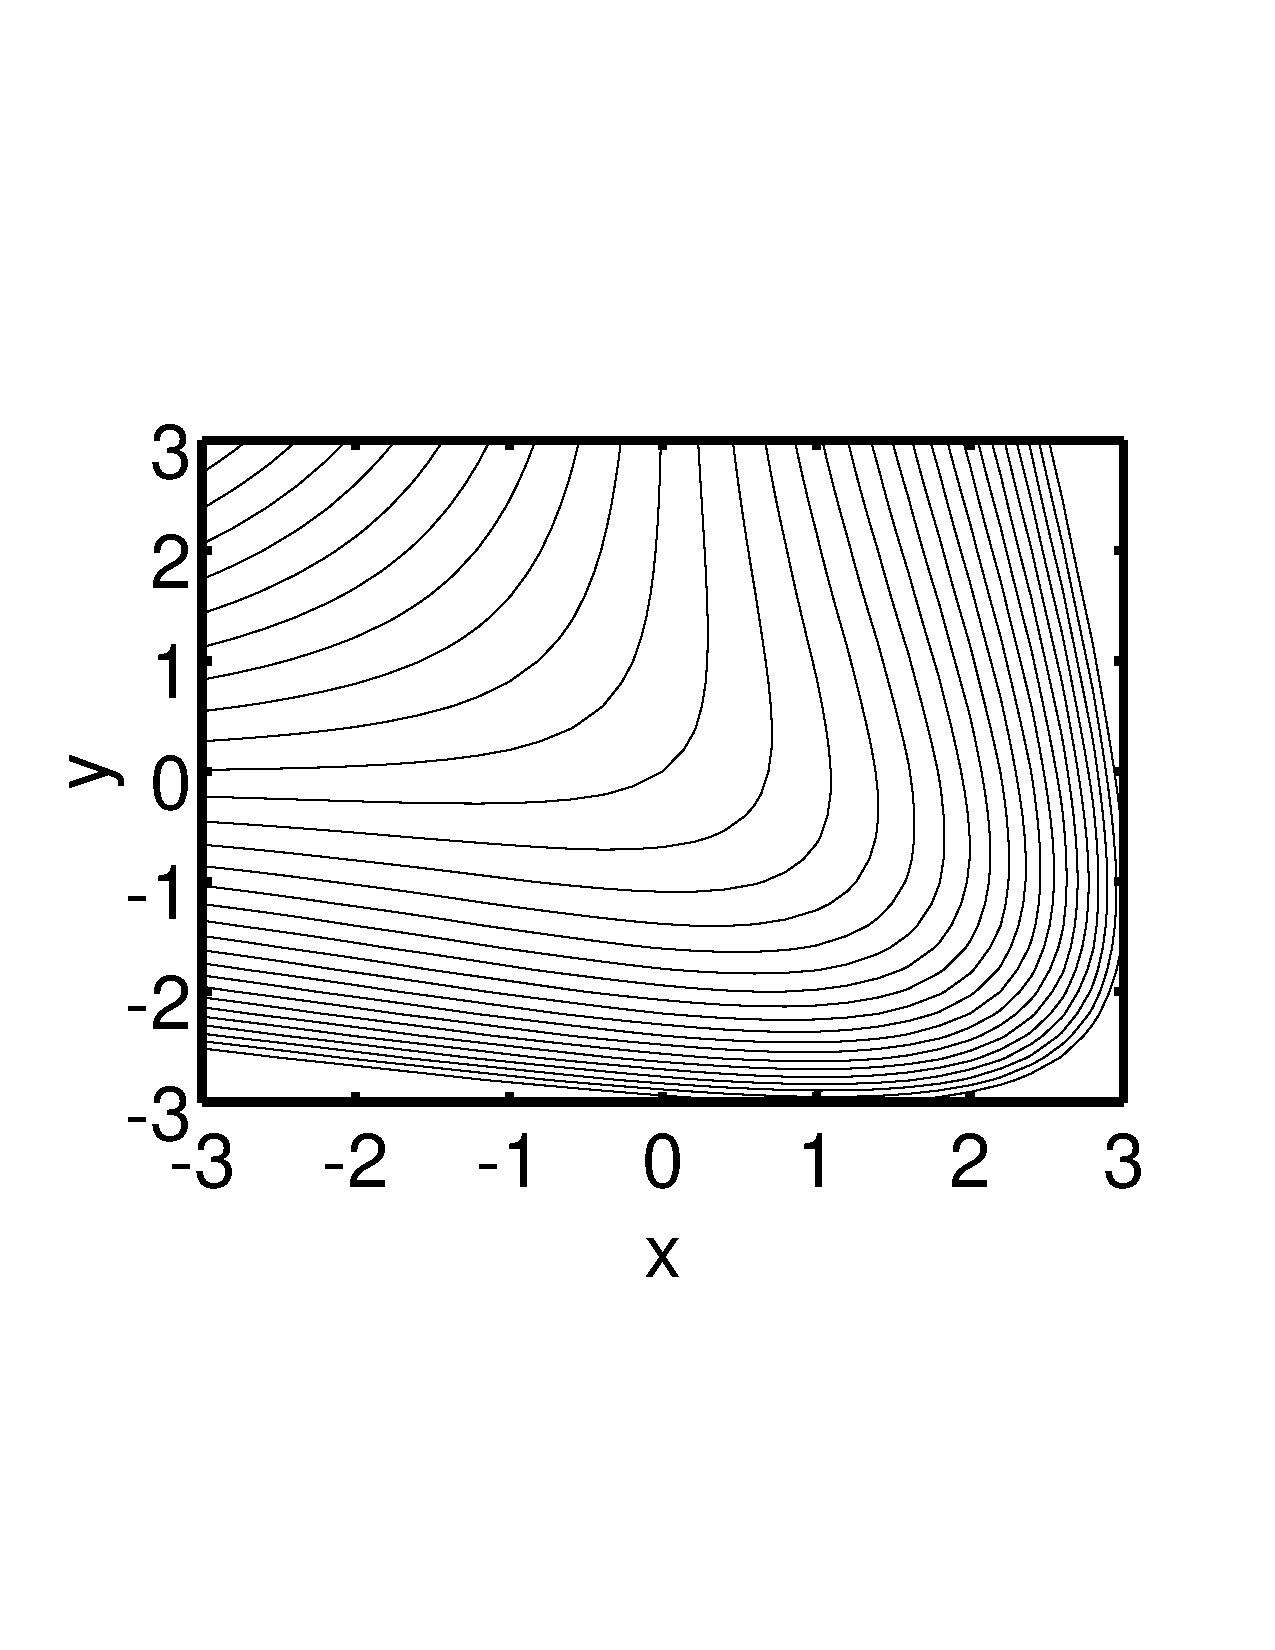
\includegraphics[height=3in]{integratingFactor}
\caption{مثال \حوالہ{مثال_سادہ_اول_جزو_تکمل_حصول}}
\label{شکل_مثال_سادہ_اول_جزو_تکمل_حصول}
\end{figure}
\انتہا{مثال}
%===========================

\حصہء{سوالات}
سوال \حوالہ{سوال_سادہ_اول_جزو_تکمل_الف} تا سوال \حوالہ{سوال_سادہ_اول_جزو_تکمل_ب} کو قطعیت کے لئے پرکھیں اور حل کریں۔غیر قطعی صورت میں دیا گیا جزو تکمل استعمال کریں یا اس کو بھی حاصل کریں۔جہاں ابتدائی معلومات دی گئی ہو، وہاں مخصوص حل حاصل کریں۔

\ابتدا{سوال}\شناخت{سوال_سادہ_اول_جزو_تکمل_الف}
\begin{align*}
2xy \dif x+x^2\dif y=0
\end{align*}
جواب:\عددی{y=\tfrac{c}{x^2}}
\انتہا{سوال} 
%===================
\ابتدا{سوال}
\begin{align*}
x^2\dif x+y\dif y=0
\end{align*}

جواب:\عددی{2x^3+3y^2=c}
\انتہا{سوال}
%============================
\ابتدا{سوال}
\begin{align*}
[\sin x+(x+y^3)\cos x]\dif x+3y^2\sin x \dif y=0
\end{align*}

جواب:\عددی{\sin x (x+y^3)}
\انتہا{سوال}
%===========================
\ابتدا{سوال}
\begin{align*}
(y+1)\dif x+(x+1)\dif y=0
\end{align*}

جواب:\عددی{x+xy+y=c}
\انتہا{سوال}
%=============================
\ابتدا{سوال}
\begin{align*}
(e^y+ye^x+y)\dif x+(xe^y+e^x+x)\dif y=0
\end{align*}

جواب:\عددی{xe^y+xy+ye^x}

\انتہا{سوال}
%=========================
\ابتدا{سوال}
\begin{align*}
\frac{y^2+4x}{x}\dif x+2y\dif y=0
\end{align*}

جواب:\عددی{F=x}، \عددی{u=(2x+y^2)x=c}
\انتہا{سوال}
%=============================
\ابتدا{سوال}
\begin{align*}
ye^x(2x+1+2y^2)\dif x+e^x(x+2y)\dif y=0
\end{align*}

جواب:\عددی{F=e^x}، \عددی{ye^{2x}(x+y)=c}
\انتہا{سوال}
%=============================
\ابتدا{سوال}
\begin{align*}
(2y^2+2xy+y)\dif x+(2y+x)\dif y=0
\end{align*}

جواب:\عددی{F=e^{2x}}، \عددی{e^{2x}(y^2+xy)=c}
\انتہا{سوال}
%=============================

\ابتدا{سوال}
\begin{align*}
y\dif x+(2xy-e^{-2y})\dif x=0, \quad y(1)=1
\end{align*}

جواب:\عددی{F=\tfrac{e^{2y}}{y}}، \عددی{xe^{2y}-\ln y=e^2}
\انتہا{سوال}
%==============
\ابتدا{سوال}
\begin{align*}
3(y+1)\dif x=2x\dif y,\quad y(1)=3,\quad F=\frac{y+1}{x^4}
\end{align*}

جواب:\عددی{y+1=4x^{\tfrac{3}{2}}}
\انتہا{سوال}
%=================
\ابتدا{سوال}
\begin{align*}
y\dif x+[y+\tan(x+y)]\dif y=0,\quad y(0)=\tfrac{\pi}{2},\quad F=\cos(x+y)
\end{align*}

جواب:\عددی{y\sin(x+y)=\tfrac{\pi}{2}}
\انتہا{سوال}
%=================
\ابتدا{سوال}\شناخت{سوال_سادہ_اول_جزو_تکمل_ب}
\begin{align*}
(a+1)y\dif x+(b+1)x \dif y=0,\quad y(1)=1, \quad F=x^ay^b
\end{align*}

جواب:\عددی{x^{a+1}y^{b+1}=0}
\انتہا{سوال}
%====================
\ابتدا{سوال}
جزو تکمل کو مزید بہتر سمجھنے کی خاطر  کسی بھی تفاعل مثلاً \عددی{u=e^{2x}(y^2+xy)=c} کے مکمل تفرق کو \عددی{M\dif +N\dif y=0} صورت میں لکھیں یعنی
 \عددی{e^{2x} (2y^2+2xy+y)\dif x+e^{2x}(2y+x)\dif y=0} جو قطعی مساوات ہے۔تفرقی مساوات کو \عددی{e^{2x}} سے تقسیم کرنے سے غیر قطعی مساوات 
\عددی{(2y^2+2xy+y)\dif x+(2y+x)\dif y=0} ملتا ہے۔۔اس غیر قطعی مساوات کو \عددی{e^{2x}} سے ضرب دیتے ہوئے قطعی بنایا جا سکتا ہے لہٰذا \عددی{e^{2x}} اس غیر قطعی مساوات کا جزو تکمل ہے۔
\انتہا{سوال}
%======================

\حصہ{خطی سادہ تفرقی مساوات۔ مساوات برنولی}
ایسے سادہ درجہ اول تفرقی مساوات جنہیں درج ذیل صورت میں لکھنا ممکن ہو \اصطلاح{خطی}\فرہنگ{خطی!سادہ تفرقی مساوات}\حاشیہب{linear}\فرہنگ{linear!ordinary differential equations} کہلاتے ہیں
\begin{align}\label{مساوات_سادہ_اول_خطی}
y'+p(x)y=r(x)
\end{align}
جبکہ ایسے مساوات جنہیں الجبرائی ترتیب دیتے ہوئے درج بالا صورت میں لکھنا ممکن نہ ہو \اصطلاح{غیر خطی} کہلاتے ہیں۔

خطی مساوات \حوالہ{مساوات_سادہ_اول_خطی} کی بنیادی خاصیت یہ ہے کہ اس میں تابع متغیرہ \عددی{y} اور تابع متغیرہ کا تفرق \عددی{y'} دونوں خطی ہیں جبکہ \عددی{p(x)} اور \عددی{r(x)} غیر تابع متغیرہ \عددی{x} کے \موٹا{کوئی} بھی تفاعل ہو سکتے ہیں۔اگر غیر تابع متغیرہ وقت ہو تب \عددی{x} کی جگہ \عددی{t} لکھا جاتا ہے۔

مساوات \حوالہ{مساوات_سادہ_اول_خطی} خطی مساوات کی معیاری صورت ہے جس کے پہلے رکن \عددی{y'} کا جزو ضربی اکائی ہے۔ایسی مساوات جس میں \عددی{y'} کی بجائے \عددی{f(x)y'} پایا جاتا ہو کو \عددی{f(x)} سے تقسیم کرتے ہوئے، اس کی معیاری صورت حاصل کی جا سکتی ہے۔ یوں خطی مساوات 
\عددی{(x+\sqrt{x})y'+y\sec x=e^x} کو \عددی{(x+\sqrt{x})} سے تقسیم کرتے ہوئے  اسے معیاری صورت \عددی{y'+\tfrac{\sec x}{x+\sqrt{x}}y=\tfrac{e^x}{x+\sqrt{x}}} میں لکھا جا سکتا ہے۔

دائیں ہاتھ \عددی{r(x)} \اصطلاح{قوت}\فرہنگ{قوت}\حاشیہب{force}\فرہنگ{force} کو ظاہر کر سکتی ہے جبکہ مساوات کا حل \عددی{y(x)} \اصطلاح{ہٹاو}\فرہنگ{ہٹاو}\حاشیہب{displacement}\فرہنگ{displacement} ہو سکتا ہے۔اسی طرح \عددی{r(x)} \اصطلاح{برقی دباو}\فرہنگ{برقی دباو}\حاشیہب{voltage}\فرہنگ{voltage} ہو سکتا ہے جبکہ \عددی{y(x)} \اصطلاح{برقی رو}\فرہنگ{برقی رو}\حاشیہب{current}\فرہنگ{current} ہو سکتی ہے۔ انجینئری میں \عددی{r(x)} کو عموماً \اصطلاح{درآیدہ}\فرہنگ{درآیدہ}\حاشیہب{input}\فرہنگ{input} یا \اصطلاح{جبری تفاعل}\فرہنگ{جبری تفاعل}\حاشیہب{forcing function}\فرہنگ{forcing function} کہتے ہیں جبکہ \عددی{y(x)} کو \اصطلاح{ماحصل}\فرہنگ{ماحصل}\حاشیہب{output}\فرہنگ{output} یا \اصطلاح{رد عمل}\فرہنگ{رد عمل}\حاشیہب{response}\فرہنگ{response} کہتے ہیں۔  
%================================

\جزوحصہء{متجانس خطی سادہ تفرقی مساوات}\شناخت{حصہ_سادہ_اول_متجانس_خطی}
ہم مساوات \حوالہ{مساوات_سادہ_اول_خطی} کو خطہ \عددی{a<x<b} میں حل کرنا چاہتے ہیں۔اس خطے کو \عددی{J} کہا جائے گا۔پہلے اس مساوات کی سادہ صورت حل کرتے ہیں جس میں \عددی{J} پر  تمام \عددی{x} کے لئے \عددی{r(x)} صفر کے برابر ہو۔ (اس کو بعض اوقات \عددی{r(x)\equiv 0} لکھا جاتا ہے۔) ایسی صورت میں مساوات \حوالہ{مساوات_سادہ_اول_خطی} درج ذیل صورت اختیار کرے گی 
\begin{align}\label{مساوات_سادہ_اول_ہم_جنسی_خطی_الف}
y'+p(x)y=0
\end{align}
جس کو \اصطلاح{متجانس}\فرہنگ{متجانس}\حاشیہب{homogeneous}\فرہنگ{homogeneous!linear ordinary differential equation} مساوات کہتے ہیں۔متغیرات علیحدہ کرتے ہوئے حل کرتے ہیں۔
\begin{align*}
\frac{\dif y}{y}=-\=p(x)\dif x,\quad \ln \abs{y}=-\int p(x) \dif x+c_1
\end{align*}
دونوں اطراف کا قوت نمائی لیتے ہوئے متجانس خطی مساوات \حوالہ{مساوات_سادہ_اول_ہم_جنسی_خطی_الف} کا حل حاصل ہوتا ہے۔
\begin{align}\label{مساوات_سادہ_اول_متجانس_حل_الف}
y(x)=ce^{-\int p(x)\dif x},\quad (c=\mp e^{c_1}\quad  \text{جب} \quad  y \lessgtr 0)
\end{align} 
یہاں \عددی{c=0} بھی چننا جا سکتا ہے جو \اصطلاح{غیر اہم حل}\فرہنگ{غیر اہم حل}\فرہنگ{حل!غیر اہم}\حاشیہب{trivial solution}\فرہنگ{trivial solution}\فرہنگ{solution!trivial} (یعنی \اصطلاح{صفر حل}) \عددی{y(x)=0} دیتا ہے۔
%====================

\جزوحصہء{غیر متجانس خطی سادہ تفرقی مساوات}
اب مساوات \حوالہ{مساوات_سادہ_اول_خطی} کو اس صورت میں حل کرتے ہیں جب \عددی{r(x) \not \equiv 0} ہو یعنی \عددی{J} پر کہیں کہیں یا پورے خطے پر  \عددی{r(x)} غیر صفر ہو۔ایسی صورت میں مساوات \حوالہ{مساوات_سادہ_اول_خطی} \اصطلاح{غیر متجانس}\فرہنگ{غیر متجانس}\حاشیہب{heterogeneous}\فرہنگ{heterogeneous} کہلاتا ہے۔غیر متجانس مساوات کی خوشگوار خاصیت یہ ہے کہ اس کا جزو تکمل \عددی{F(x)} صرف \عددی{x} پر منحصر ہوتا ہے لہٰذا اس کو مسئلہ \حوالہ{مسئلہ_سادہ_اول_جزو_تکمل_الف} کی مدد سے حاصل کیا جا سکتا ہے۔جزو تکمل کو حاصل کرتے ہیں۔غیر قطعی مساوات \حوالہ{مساوات_سادہ_اول_خطی} کو ترتیب دے کر \عددی{F} سے ضرب دیتے ہوئے قطعی مساوات حاصل کرتے ہیں
\begin{align*}
(py-r)\dif x+\dif y&=0,\quad F(py-r)\dif x+F\dif y=0
\end{align*}
جس سے مساوات \حوالہ{مساوات_سادہ_اول_قطعی_تفرقی_شرط} کی مدد سے درج ذیل ملتا ہے۔
\begin{align*}
\frac{\partial}{\partial y} [F(py-r)]=\frac{\partial F}{\partial x}\quad  \text{یعنی} \quad Fp=\frac{\partial F}{\partial x}
\end{align*}
متغیرات علیحدہ کرتے ہوئے تکمل لیتے ہوئے \عددی{F} حاصل کرتے ہیں۔
\begin{align*}
\frac{\dif F}{F}=p\dif x, \quad \ln \abs{F}=h(x)=\int p(x)\dif x \quad  \text{لہٰذا}\quad  F=e^h
\end{align*}
مساوات \حوالہ{مساوات_سادہ_اول_خطی} کو جزو تکمل \عددی{F} سے ضرب دیتے  اور \عددی{\tfrac{\dif h}{\dif x}=p} لکھتے ہوئے درج ذیل ملتا ہے
\begin{align*}
e^h y'+e^h h' y=e^h r \quad \text{یعنی}\quad  \left(e^h y\right)'=e^h r
\end{align*}
جس کا تکمل لیتے ہیں۔
\begin{align*}
e^h y=\int e^h r \dif x+c
\end{align*}
دونوں اطراف کو \عددی{e^h} سے تقسیم کرتے ہوئے غیر متجانس مساوات \حوالہ{مساوات_سادہ_اول_خطی} کا حل ملتا ہے۔
\begin{align}\label{مساوات_سادہ_اول_متجانس_خطی_حل_الف}
y=e^{-h}\left(\int e^h r \dif x+c\right), \quad h=\int p(x)\dif x
\end{align}
یوں مساوات \حوالہ{مساوات_سادہ_اول_خطی} کا حل درج بالا تکمل سے حاصل کیا جا سکتا ہے جو نسبتاً آسان ثابت ہوتا ہے۔اگر درج بالا تکمل بھی مشکل ثابت ہو تب تفرقی مساوات کا حل اعدادی ترکیب سے حاصل کیا جا سکتا ہے۔یہاں بتلاتا چلوں (سوال \حوالہ{سوال_سادہ_اول_برنولی_الف} دیکھیں) کہ \عددی{h} کے حصول میں تکمل کا مستقل کوئی کردار ادا نہیں کرتا لہٰذا اسے  صفر تصور کیا جاتا ہے۔

مساوات \حوالہ{مساوات_سادہ_اول_متجانس_خطی_حل_الف} کا تکمل درآیدہ \عددی{r(x)} پر منحصر ہے جبکہ ابتدائی معلومات تکمل کا مستقل \عددی{c} تعین کرتی ہیں۔اس مساوات کو درج ذیل لکھتے ہوئے 
\begin{align}\label{مساوات_سادہ_اول_متجانس_خطی_حل_ب}
y=e^{-h}\int e^h r \dif x+ce^{-h}
\end{align}
ہم دیکھتے ہیں کہ
\begin{align}
\text{کل ماحصل}=\text{درآیدہ سے پیدا رد عمل}+\text{ابتدائی معلومات سے پیدا رد عمل}
\end{align}

%=========================

\ابتدا{مثال}
ابتدائی قیمت تفرقی مساوات کو حل کریں۔
\begin{align*}
y'+y\cot x=2x\cosec x,\quad y\left(\frac{\pi}{2}\right)=0
\end{align*}

حل:یہاں \عددی{p=\cot x} اور \عددی{r=\cosec x} ہیں۔
\begin{align*}
h(x)=\int \cot x \dif x=\ln \abs{\sin x}
\end{align*}
یوں مساوات \حوالہ{مساوات_سادہ_اول_متجانس_خطی_حل_الف} میں
\begin{align*}
e^h=\sin x, \quad e^{-h}=\cosec x, \quad e^h r= (\sin x) (2x\cosec x)=2x
\end{align*}
ہیں لہٰذا عمومی حل
\begin{align*}
y=\cosec x \left(\int 2x\dif x +c\right)=\cosec x (x^2+c)
\end{align*}
ہو گا۔ابتدائی معلومات پر کرتے ہوئے  \عددی{c=-\tfrac{\pi^2}{4}} ملتا ہے لہٰذا مخصوص حل درج ذیل ہے
\begin{align*}
y=\cosec x \left(x^2-\frac{\pi^2}{4}\right)
\end{align*}
جس میں \عددی{x^2\cosec x} درآیدہ کا پیدا کردہ رد عمل ہے جبکہ \عددی{-\tfrac{\pi^2}{4}\cosec x} ابتدائی معلومات کا پیدا کردہ رد عمل ہے۔
\انتہا{مثال}
%==========================
\ابتدا{مثال}\شناخت{مثال_سادہ_اول_برقی_دور_الف} \quad برقی دور\\
شکل \حوالہ{شکل_مثال_سادہ_اول_برقی_دور_الف} میں \اصطلاح{مزاحمت}\فرہنگ{مزاحمت}\حاشیہب{resistance}\فرہنگ{resistance} \عددی{R} اور \اصطلاح{امالہ}\فرہنگ{امالہ}\حاشیہب{inductor}\فرہنگ{inductor} \عددی{L} سلسلہ وار جڑے ہیں۔اس دور کو \اصطلاح{سلسلہ وار}\فرہنگ{سلسلہ وار دور}\حاشیہب{series circuit}\فرہنگ{series circuit} \عددی{RL} دور کہتے ہیں۔لمحہ \عددی{t=0} پر \اصطلاح{برقی دباو}\فرہنگ{برقی دباو}\حاشیہب{electric voltage}\فرہنگ{voltage} \عددی{E} برقی دور پر لاگو کیا جاتا ہے جو دور میں \اصطلاح{برقی رو}\فرہنگ{برقی رو}\حاشیہب{electric current}\فرہنگ{current} \عددی{I(t)} کو جنم دیتا ہے۔ابتدائی رو صفر \عددیء{I(0)=0} کے برابر ہے۔

طبعی معلومات: مزاحمت کی اکائی \اصطلاح{اوہم}\فرہنگ{اوہم}\حاشیہب{Ohm}\فرہنگ{Ohm} \عددی{\si{\ohm}}  اور امالہ کی اکائی \اصطلاح{ہینری}\فرہنگ{ہینری}\حاشیہب{Henry}\فرہنگ{Henry} \عددی{\si{\henry}} ہے۔\اصطلاح{قانون اوہم}\فرہنگ{قانون اوہم}\حاشیہب{Ohm's law}\فرہنگ{Ohm's law} کے تحت مزاحمت \عددی{R} میں رو \عددی{I} اور دباو \عددی{v_R} کا تعلق \عددی{v_R=IR} ہے۔اسی طرح امالہ میں رو اور دباو \عددی{v_L} کا تعلق \عددی{v_L=L\tfrac{\dif I}{\dif t}} ہے۔ \اصطلاح{کرخوف قانون دباو}\فرہنگ{کرخوف!قانون دباو}\حاشیہب{Kirchoff's voltage law}\فرہنگ{Kirchoff's law!voltage} کے تحت ان برقی دباو کا مجموعہ درآیدہ دباو \عددی{E} کے برابر ہو گا۔ 
\begin{figure}
\centering
\begin{subfigure}{0.5\textwidth}
\centering
\begin{tikzpicture}[american voltages]
\draw(0,0) to [american voltage source,l={$\substack{\displaystyle E \hfill \\ \displaystyle \SI{50}{\volt}}$}]++(0,\yy) to [resistor,l={$\substack{\displaystyle R\hfill \\ \displaystyle \SI{100}{\ohm}}$},i={$I(t)$},v={$v_R$}]++(\xx,0) to [inductor,l_={$\substack{\displaystyle L \hfill \\ \displaystyle \SI{0.5}{\henry}}$},v^<={$v_L$}]++(0,-\yy) to [short]++(-\xx,0);
\end{tikzpicture}
\caption*{(الف)}
\end{subfigure}%
\begin{subfigure}{0.5\textwidth}
\centering
\begin{tikzpicture}
\begin{axis}[small,axis lines*=middle,xlabel={$t$},ylabel={$I(t)$},xtick={0.01,0.02,0.03},xticklabels={$0.01$,$0.02$,$0.03$},ytick={0,0.25,0.5,0.75},yticklabels={$0$,$0.25$,$\frac{E}{R}$,$0.75$},ylabel style={rotate=-90},ylabel style={at={(axis description cs:0,1.05)}},scaled x ticks=false,scaled y ticks=false]
\addplot[thick,domain=0:0.035]{50/100*(1-e^(-200*x))};
\addplot[domain=0:0.035]{0.5-0.25*e^(-200*x)};
\addplot[domain=0:0.035]{0.5+0.25*e^(-200*x)};
\end{axis}
\end{tikzpicture}
\caption*{(ب)}
\end{subfigure}%
\caption{مثال \حوالہ{مثال_سادہ_اول_برقی_دور_الف} کا سلسلہ وار برقی دور۔}
\label{شکل_مثال_سادہ_اول_برقی_دور_الف}
\end{figure}


حل:یہاں غیر تابع متغیرہ وقت \عددی{t} ہے جبکہ تابع متغیرہ رو \عددی{I(t)} ہے۔ کرخوف کے قانون کے تحت 
\begin{align*}
v_L+v_R=E, \quad L I'+RI=E, \quad I'+\frac{R}{L}I=\frac{E}{L}
\end{align*}
لکھا جائے گا جہاں آخری قدم پر \عددی{L} سے تقسیم کرتے ہوئے مساوات کو معیاری صورت میں لکھا گیا ہے۔اس کو مساوات \حوالہ{مساوات_سادہ_اول_متجانس_خطی_حل_الف} کی مدد سے حل کرتے ہیں جہاں \عددی{x} کی جگہ \عددی{t} اور \عددی{y} کی جگہ \عددی{I} استعمال ہو گا۔یہاں \عددی{p=\tfrac{R}{L}} اور \عددی{r=\tfrac{E}{L}} ہیں لہٰذا \عددی{h=\tfrac{R}{L}t} ہو گا اور عمومی حل
\begin{align*}
I=e^{-\frac{R}{L}t}\left(\int e^{\frac{R}{L}t}  \frac{E}{L} \dif x+c\right)
\end{align*}
لکھا جائے گا۔تکمل لیتے ہوئے درج ذیل ملتا ہے۔
\begin{align}\label{مساوات_سادہ_اول_برقی_مزاحمت_امالہ_سلسلہ_وار}
I=e^{-\frac{R}{L}t}\left(\frac{E}{L} \frac{e^{\frac{R}{L}}t}{\frac{R}{L}}+c\right)=\frac{E}{R}+ce^{-\frac{R}{L}t}
\end{align}
شکل \حوالہ{شکل_مثال_سادہ_اول_برقی_دور_الف}-الف میں پرزوں کی قیمتیں دی گئی ہیں جن سے \عددی{\tfrac{E}{R}=\tfrac{50}{100}=0.5} اور
 \عددی{\tfrac{R}{L}=\tfrac{100}{0.5}=200} ملتا ہے لہٰذا عمومی حل کو درج ذیل لکھا جا سکتا ہے۔
\begin{align}
I=0.5+ce^{-200t}
\end{align} 
مساوات \حوالہ{مساوات_سادہ_اول_برقی_مزاحمت_امالہ_سلسلہ_وار} میں ابتدائی معلومات پر کرتے ہوئے \عددی{c} کی قیمت حاصل ہوتی ہے۔ اس مساوات میں \عددی{ce^{-\tfrac{R}{L}t}} جزو \عددی{t \to \infty} پر صفر کے برابر ہو گا لہٰذا کافی دیر بعد رو پہلے جزو \عددی{\tfrac{E}{R}} کے برابر ہو گی جسے رو کی \اصطلاح{برقرار حال}\فرہنگ{برقرار حال}\حاشیہب{steady state}\فرہنگ{steady state} قیمت کہتے ہیں۔یہ ایک اہم نتیجہ ہے جس کے  تحت کافی دیر بعد رو کی قیمت کا دارومدار ابتدائی معلومات پر منحصر نہیں ہے۔رو کتنی جلدی برقرار حال قیمت اختیار کرتی ہے، اس کا دارومدار \عددی{\tfrac{R}{L}} کی قیمت پر ہے۔

مساوات \حوالہ{مساوات_سادہ_اول_برقی_مزاحمت_امالہ_سلسلہ_وار} میں ابتدائی معلومات \عددی{I(0)=0} پر کرتے  \عددی{0=0.5+ce^0} ہوئے \عددی{c=-0.5} ملتا ہے لہٰذا مخصوص حل درج ذیل ہو گا جس کو شکل \حوالہ{شکل_مثال_سادہ_اول_برقی_دور_الف}-ب میں موٹی لکیر سے دکھایا گیا ہے۔شکل میں ابتدائی قیمت \عددی{I(0)=0.25} اور \عددی{I(0)=0.75} سے حاصل مخصوص حل بھی دکھائے گئے ہیں۔
\begin{align}
I(t)=0.5(1-e^{-200t})
\end{align}
\انتہا{مثال}
%==========================
\ابتدا{مثال}\شناخت{مثال_سادہ_اول_غدود_درقیہ}\quad جسم میں ہارمونز کی مقدار\\
جسم میں موجود \اصطلاح{غدود}\فرہنگ{غدود}\حاشیہب{gland}\فرہنگ{gland} یعنی  \اصطلاح{گلٹی}\فرہنگ{گلٹی}، خون میں مختلف مرکبات\اصطلاح{(ہارمونز)}\فرہنگ{ہارمونز}\حاشیہب{hormones}\فرہنگ{hormones} خارج کرتے ہوئے مختلف نظام کو قابو کرتے ہیں۔تصور کریں کہ خون سے ایک مخصوص ہارمون مسلسل ہٹایا جاتا ہے۔ہٹانے کی شرح اس لمحے موجود ہارمون کی مقدار کے راست تناسب ہے۔ساتھ ہی ساتھ تصور کریں کہ روزانہ غدود اس ہارمون کو خون میں ایک مخصوص انداز سے خارج کرتی ہے۔خون میں موجود ہارمون کی نمونہ کشی کرتے ہوئے تفرقی مساوات کا عمومی حل حاصل کریں۔صبح چھ بجے خون میں ہارمون کی مقدار \عددی{y_0} لیتے ہوئے مخصوص حل حاصل کریں۔  

حل:پہلا قدم: نمونہ کشی:\quad چوبیس گھنٹوں میں خارج ہونے کے عمل کو \عددی{a+b\sin (\tfrac{2\pi t}{24})} سے ظاہر کرتے ہیں۔چونکہ خون میں ہارمون خارج ہونے سے خون میں ہارمون کی مقدار بڑھتی ہے لہٰذا \عددی{a\ge b} ہو گا۔یوں خارج کردہ ہارمون کی مقدار مثبت ہو گی۔کسی بھی لمحے خون میں ہارمون کی مقدار کی تبدیلی کی شرح، اس لمحے خون میں ہارمون کے داخل ہونے کی مقدار اور اس کی ہٹائی جانے والی مقدار میں فرق کے برابر ہو گا۔یوں مسئلے کا تفرقی مساوات درج ذیل ہو گا۔
\begin{align}
\frac{\dif y(t)}{\dif t}=a+b\sin\left(\frac{2\pi t}{24}\right)-k y(t) \quad \text{یعنی}\quad y'-ky=a+b\sin \omega t,\quad \omega =\frac{2\pi}{24}
\end{align}
دوسرا قدم: عمومی حل:\quad یہاں \عددی{p=k} ہے لہٰذا \عددی{h=\int k\dif t=kt} ہو گا۔اسی طرح \عددی{r=a+b\sin \omega t} ہے لہٰذا مساوات \حوالہ{مساوات_سادہ_اول_متجانس_خطی_حل_الف} سے عمومی حل درج ذیل ہو گا جس کو \اصطلاح{تکمل بالحصص}\فرہنگ{تکمل!بالحصص}\حاشیہب{integration by parts}\فرہنگ{integration!by parts} حل کیا گیا ہے
\begin{align*}
y&=e^{-kt}\int e^{kt} (a+b\sin \omega t) \dif t+ce^{-kt}\\
&=e{-kt}e^{kt}\left[\frac{a}{k}+\frac{b}{k^2+\omega^2}(k\cos \omega t+\omega \sin \omega t)\right]+ce^{-kt}\\
&=\frac{a}{k}+\frac{b}{k^2+\omega^2}(k\cos \omega t+\omega \sin \omega t)+ce^{-kt}
\end{align*}
عمومی حل کا آخری جزو وقت بڑھنے سے آخر کار صفر ہو جاتا ہے۔یوں \اصطلاح{برقرار حل}\فرہنگ{برقرار حل}\حاشیہب{steady state response}\فرہنگ{steady state response} بقایا اجزاء پر مشتمل ہے۔

آخر قدم:مخصوص حل:\quad صبح چھ بجے کو لمحہ \عددی{t=0} تصور کرتے ہوئے ابتدائی معلومات کو \عددی{y(0)=y_0} لکھا جا سکتا ہے۔ان قیمتوں کو عمومی حل میں پر کرتے ہوئے \عددی{c} کی قیمت حاصل کرتے ہیں۔
\begin{align*}
y_0 &=\frac{a}{k}+\frac{b}{k^2+\omega^2}(k\cos 0+\omega \sin 0)+ce^{0}, \quad \text{یعنی}\quad c=y_0-\frac{a}{k}-\frac{bk}{k^2+\omega^2}
\end{align*}
اس طرح مخصوص حل درج ذیل ہو گا۔مخصوص حل کو \عددی{a=1}، \عددی{b=1}، \عددی{k=0.04} اور \عددی{y_0=0} لیتے ہوئے  جسے شکل \حوالہ{شکل_مثال_سادہ_اول_غدود_درقیہ} میں دکھایا گیا ہے۔ شکل-ب میں \عددی{y_0=50} لیا گیا ہے۔آپ دیکھ سکتے ہیں کہ خون میں ہارمون کی مقدار بہت جلد ایک مخصوص اوسط قیمت پر پہنچ پاتی ہے۔
\begin{align*}
y=\frac{a}{k}+\frac{b}{k^2+\omega^2}(k\cos \omega t+\omega \sin \omega t)+(y_0-\frac{a}{k}-\frac{bk}{k^2+\omega^2})e^{-kt}
\end{align*}
%
\begin{figure}
\centering
\begin{subfigure}{0.5\textwidth}
\centering
\begin{tikzpicture}
\pgfmathsetmacro{\a}{2*pi/24}
\pgfmathsetmacro{\b}{2*pi/24}
\pgfmathsetmacro{\w}{2*pi/24}
\pgfmathsetmacro{\wa}{360/24}
\pgfmathsetmacro{\k}{0.04}
\pgfmathsetmacro{\ya}{0}
\begin{axis}[small,axis lines*=middle,ymin=0,ymax=55,xmin=0,xlabel={$t$},ylabel={$y(t)$},ylabel style={rotate=-90},ylabel style={at={(axis description cs:0,1.05)}}]
\addplot[domain=0:300,samples=400]{1/\k+(\k*cos(\wa*x)+\w*sin(\wa*x))/(\k^2+\w^2)+(\ya-1/\k-\k/(\k^2+\w^2))*e^(-\k*x)};
\end{axis}
\end{tikzpicture}
\caption*{(الف)}
\end{subfigure}%
\begin{subfigure}{0.5\textwidth}
\centering
\begin{tikzpicture}
\pgfmathsetmacro{\w}{2*pi/24}
\pgfmathsetmacro{\wa}{360/24}
\pgfmathsetmacro{\k}{0.04}
\pgfmathsetmacro{\ya}{50}
\begin{axis}[small,axis lines*=middle,ymin=0,ymax=55,xmin=0,xlabel={$t$},ylabel={$y(t)$},ylabel style={rotate=-90},ylabel style={at={(axis description cs:0,1.05)}}]
\addplot[domain=0:300,samples=400]{1/\k+(\k*cos(\wa*x)+\w*sin(\wa*x))/(\k^2+\w^2)+(\ya-1/\k-\k/(\k^2+\w^2))*e^(-\k*x)};
\end{axis}
\end{tikzpicture}
\caption*{(ب)}
\end{subfigure}%
\caption{مثال \حوالہ{مثال_سادہ_اول_غدود_درقیہ}: خون میں ہارمون کی مقدار بالمقابل وقت۔}
\label{شکل_مثال_سادہ_اول_غدود_درقیہ}
\end{figure}
\انتہا{مثال}
%=============================

\جزوحصہء{حصول خطی مساوات بذریعہ تخفیف۔ برنولی مساوات}
ایسے بہت سارے نظام ہیں جن کے غیر خطی سادہ تفرقی مساوات کو خطی بنایا جا سکتا ہے۔ان میں \اصطلاح{برنولی مساوات}\فرہنگ{برنولی مساوات}\حاشیہب{Bernoulli equation}\فرہنگ{Bernoulli!equation} 
\begin{align}\label{مساوات_سادہ_اول_برنولی_الف}
y'+p(x)y=g(x)y^a,\quad \text{\RL{$a$\, حقیقی عدد ہے}}
\end{align}
انتہائی اہم\حاشیہد{یعقوب برنولی (1654-1705): سوئزرلینڈ کے برنولی خاندان نے دنیا کو کئی اہم ریاضی داں دیے۔ یعقوب برنولی ان میں سر فہرست ہے۔انہوں نے علم الامکانیات میں بہت کام کیا۔قوت نمائی کا مستقل \عددی{e} بھی انہوں نے دریافت کیا۔} ہے۔برنولی مساوات \عددی{a=0} اور \عددی{a=1} کی صورت میں خطی ہے۔ اس کے علاوہ یہ غیر خطی ہے۔آئیں اس کو تبدیل کرتے ہوئے خطی مساوات حاصل کریں۔ہم
\begin{align*}
u(x)=[y(x)]^{1-a}
\end{align*}
کا تفرق لیتے ہوئے اس میں مساوات \حوالہ{مساوات_سادہ_اول_برنولی_الف} سے \عددی{y'} پر کرتے  ہوئے ترتیب دیتے ہیں۔
\begin{align*}
u'&=(1-a)y^{-a}y'\\
&=(1-a)y^{-a}(gy^a-py)\\
&=(1-a)g-(1-a)py^{1-a}\\
&=(1-a)g-(1-a)pu
\end{align*} 
یوں خطی سادہ تفرقی مساوات 
\begin{align}
u+(1-a)u'=(1-a)g
\end{align}
حاصل ہوتی ہے۔
%=============================

\ابتدا{مثال}\شناخت{مثال_سادہ_اول_نمو_آبادی}\quad ورہلسٹ مساوات برائے نمو آبادی
درج ذیل برنولی مساوات کو \اصطلاح{ورہلسٹ}\فرہنگ{ورہلسٹ}\حاشیہب{Pierre Francois Verhulst}\فرہنگ{Verhulst equation} مساوات کہتے ہیں جو \اصطلاح{نمو آبادی}\فرہنگ{نمو آبادی}\حاشیہب{population growth}\فرہنگ{population growth} کی تفرقی مساوات ہے۔اس کو حل کریں۔ (سوال \حوالہ{سوال_سادہ_اول_وبا} کو بھی دیکھیں۔)
\begin{align}\label{مساوات_سادہ_اول_ورہلسٹ_آبادی_نمو_الف}
y'=ay-by^2
\end{align}

حل:اس کو مساوات \حوالہ{مساوات_سادہ_اول_برنولی_الف} کی صورت \عددی{y'-ay=-by^2} میں لکھ کر \عددی{a=2} ملتا ہے۔یوں ہم \عددی{u=y^{1-a}=y^{-1}} کے تفرق میں مساوات \حوالہ{مساوات_سادہ_اول_ورہلسٹ_آبادی_نمو_الف} سے \عددی{y'}  پر کرتے ہیں
\begin{align*}
u'=-y^{-2}y'=-y^{-2}(ay-by^2)=-ay^{-1}+b=-ua+b
\end{align*}
جس سے خطی سادہ تفرقی مساوات
\begin{align*}
u'+au=b
\end{align*}
حاصل ہوتا ہے۔ مساوات \حوالہ{مساوات_سادہ_اول_متجانس_خطی_حل_الف} سے عمومی حل لکھتے ہیں۔
\begin{align*}
u=\frac{b}{a}+ce^{-at}
\end{align*}
چونکہ \عددی{u=y^{-1}} ہے لہٰذا اس سے درج ذیل ملتا ہے جس کو شکل \حوالہ{شکل_مثال_سادہ_اول_نمو_آبادی} میں دکھایا گیا ہے۔
\begin{align}\label{مساوات_سادہ_اول_نمو_آبادی}
y=\frac{1}{u}=\frac{1}{\frac{b}{a}+ce^{-at}}
\end{align}
مساوات \حوالہ{مساوات_سادہ_اول_ورہلسٹ_آبادی_نمو_الف} کو دیکھ کر \عددی{y(t)=0} حل بھی لکھا جا سکتا ہے۔ 
\begin{figure}
\centering
\begin{tikzpicture}
\pgfmathsetmacro{\a}{3}
\pgfmathsetmacro{\b}{1}
\pgfmathsetmacro{\ca}{100*\b/\a}
\pgfmathsetmacro{\caa}{1*\b/\a}
\pgfmathsetmacro{\cb}{-0.25*\b/\a}
\pgfmathsetmacro{\cc}{-0.375*\b/\a}
\pgfmathsetmacro{\cd}{-0.5*\b/\a}
\pgfmathsetmacro{\ce}{0*\b/\a}
\begin{axis}[small,axis lines*=middle,xmin=0,ymin=0,xlabel={$t$},ylabel={$y$},ylabel style={rotate=-90},ylabel style={at={(axis description cs:0,1.05)}},ytick={2,3,4,6},yticklabels={$2$,$\frac{a}{b}=3$,$4$,$6$}]
\addplot[domain=0:4,samples=50]{(\b/\a+\ca*e^(-\a*x))^(-1)};
\addplot[domain=0:4,samples=50]{(\b/\a+\caa*e^(-\a*x))^(-1)};
\addplot[domain=0:4,samples=50]{(\b/\a+\cb*e^(-\a*x))^(-1)};
\addplot[domain=0:4,samples=50]{(\b/\a+\cc*e^(-\a*x))^(-1)};
\addplot[domain=0:4,samples=50]{(\b/\a+\cd*e^(-\a*x))^(-1)};
\addplot[domain=0:4,samples=50]{(\b/\a+\ce*e^(-\a*x))^(-1)};
\end{axis}
\end{tikzpicture}
\caption{مثال \حوالہ{مثال_سادہ_اول_نمو_آبادی}: نمو آبادی کا خط۔}
\label{شکل_مثال_سادہ_اول_نمو_آبادی}
\end{figure}
\انتہا{مثال}
%===============================
\ابتدا{مثال}\شناخت{مثال_سادہ_درجہ_اول_متغیرات_بدلنے_کا_طریقہ}\quad مقدار معلوم بدلنے کا طریقہ\\
مساوات \حوالہ{مساوات_سادہ_اول_متجانس_خطی_حل_الف} کو ایک دلچسپ ترکیب سے حاصل کیا جا سکتا ہے جسے \اصطلاح{مقدار معلوم بدلنے کا طریقہ}\فرہنگ{مقدار معلوم!بدلنے کا طریقہ}\حاشیہب{variation of parameter}\فرہنگ{variation of parameter} کہتے ہیں۔متجانس مساوات \عددی{y'+p(x)y=0} کا  حل \عددی{y_1=ce^{-\int p(x) \dif x}} مساوات \حوالہ{مساوات_سادہ_اول_متجانس_حل_الف} دیتا ہے جس کو \عددی{y_1=ce^{-h}} لکھتے ہیں۔تصور کریں کہ غیر متجانس مساوات \عددی{y'+p(x)y=e(x)} کا حل \عددی{y_2=uy_1} لکھا جا سکتا ہے۔یوں \عددی{y_2'=u'y_1+uy_1'} ہو گا۔غیر متجانس مساوات میں \عددی{y_2} اور \عددی{y_2'} پر کرتے ہیں۔
\begin{align*}
u'y_1+uy_1'+p uy_1=r, \quad u'y_1+u(y_1'+py_1)=r,\quad u'y_1=r
\end{align*}
چونکہ \عددی{y_1}  متجانس مساوات کا حل ہے لہٰذا آخری قدم پر \عددی{y'+py=0} پر کرتے ہوئے \عددی{u'y_1=r} حاصل کیا گیا ہے۔اس سے \عددی{u} بذریعہ تکمل حاصل کرتے ہوئے \عددی{y_2} لکھتے ہیں جو مساوات \حوالہ{مساوات_سادہ_اول_متجانس_خطی_حل_الف} ہے۔  
\begin{align*}
u=\int \frac{r}{y_1}\dif x,\quad u=\int re^{h} \dif x+c, \quad \text{لہٰذا} \quad y_2=uy_1=e^{-h}\left[\int re^{h} \dif x+c\right]
\end{align*}


\انتہا{مثال}
%=============================
\جزوحصہء{نمو آبادی}
ورہلسٹ مساوات پودوں، جانوروں اور انسانی آبادی کی نمو کو ظاہر کرتی ہے۔اس مساوات  میں \عددی{b=0} پر کرنے سے  مالتھس مساوات \حوالہ{مساوات_سادہ_اول_مالتھس_الف} ملتی ہے جو آبادی کی بے روک نمو دیتی ہے۔ورہلسٹ مساوات میں جزو \عددی{-by^2}  آبادی بے قابو بڑھنے سے روکتی ہے۔ورہلسٹ مساوات کو \عددی{y'=ay(1-\tfrac{b}{a}y)} لکھ کر آپ دیکھ سکتے ہیں کہ \عددی{\tfrac{b}{a}y<1} کی صورت میں \عددی{y'>0} ہو گا اور آبادی  اس وقت تک مسلسل بڑھے گی جب تک بڑھے گی جبکہ  \عددی{\tfrac{b}{a}y<1} ہو، \عددی{\tfrac{b}{a}y>1} کی صورت میں \عددی{y'<0} ہو گا اور آبادی اس وقت تک مسلسل گھٹے گی جب تک \عددی{\tfrac{b}{a}y<1} ہو گا۔دونوں صورتوں میں عین \عددی{\tfrac{b}{a}y=1} یعنی \عددی{y=\tfrac{a}{b}} پر آبادی میں تبدیلی رک جائے گی۔شکل \حوالہ{شکل_مثال_سادہ_اول_نمو_آبادی} میں ایسا دکھایا گیا ہے۔

ورہلسٹ نمو آبادی کی مساوات میں غیر تابع متغیرہ \عددی{t} صریحاً نہیں پایا جاتا لہٰذا  یہ \اصطلاح{خود مختار}\فرہنگ{خود مختار!مساوات} مساوات ہے۔خود مختار مساوات
\begin{align}\label{مساوات_سادہ_اول_خود_مختار}
y'=f(y)
\end{align}
کے مستقل حل پائے جاتے ہیں جنہیں \اصطلاح{متوازن حل}\فرہنگ{متوازن حل}\حاشیہب{equilibrium solution}\فرہنگ{equilibrium!solution} یا \اصطلاح{متوازن نقطے}\فرہنگ{متوازن!نقطے}\حاشیہب{equilibrium points}\فرہنگ{equilibrium!points} کہا جاتا ہے۔خود مختار مساوات میں تفاعل \عددی{f(y)} کے صفر (f(y)=0) پر \عددی{y'=0} ہو گا جس کا حل \عددی{y=c} ہے جہاں \عددی{c} تکمل کا مستقل ہے۔تفاعل کے صفر کو مساوات \حوالہ{مساوات_سادہ_اول_خود_مختار} کے \اصطلاح{فاصل نقطے}\فرہنگ{فاصل نقطے}\حاشیہب{critical points}\فرہنگ{critical points} کہتے ہیں۔مساوات \حوالہ{مساوات_سادہ_اول_ورہلسٹ_آبادی_نمو_الف} کے فاصل نقطے \عددی{y=0} اور \عددی{y=\tfrac{a}{b}} ہیں۔یوں اس مساوات کے مستقل حل \عددی{y=0} اور \عددی{y=\tfrac{a}{b}} ہیں۔متوازن حل کو دو گروہ میں تقسیم کیا جاتا ہے جنہیں \اصطلاح{مستحکم}\فرہنگ{مستحکم}\حاشیہب{stable}\فرہنگ{stable} اور \اصطلاح{غیر مستحکم}\فرہنگ{غیر مستحکم}\حاشیہب{unstable}\فرہنگ{unstable} متوازن حل کہتے ہیں۔ ان کو شکل \حوالہ{شکل_مثال_سادہ_اول_نمو_آبادی} کی مدد سے سمجھا جا سکتا ہے جہاں \عددی{y=\tfrac{a}{b}=3} مستحکم حل ہے جبکہ \عددی{y=0} غیر مستحکم حل ہیں۔
%===================================



\حصہء{سوالات}
%================================
\ابتدا{سوال}\شناخت{سوال_سادہ_اول_برنولی_الف}
مساوات \حوالہ{مساوات_سادہ_اول_متجانس_خطی_حل_الف} میں \عددی{h} کے حصول میں تکمل کا مستقل صفر لیا جا سکتا ہے۔ایسا کیوں ممکن ہے؟
\انتہا{سوال}
%============================
\ابتدا{سوال}
ثابت کریں:
\begin{align*}
e^{\ln x}=x, \quad  e^{-\ln x}=\frac{1}{x}, \quad e^{-\ln \sec x}=\cos x
\end{align*}
\انتہا{سوال}
%==============================
سوال \حوالہ{سوال_سادہ_اول_برنولی_ب} تا سوال \حوالہ{سوال_سادہ_اول_برنولی_پ} کے عمومی حل تلاش کریں۔ابتدائی معلومات کی صورت میں مخصوص حل حاصل کریں اور اس کا خط کھینچیں۔

\ابتدا{سوال}\شناخت{سوال_سادہ_اول_برنولی_ب}
\begin{align*}
y'-y=2
\end{align*}

جواب:\عددی{y=ce^x-2}
\انتہا{سوال}
%==========================
\ابتدا{سوال}
\begin{align*}
y'-4y=2x
\end{align*}

جواب:\عددی{y=ce^{4x}-\tfrac{x}{2}-\tfrac{1}{8}}
\انتہا{سوال}
%===========================
\ابتدا{سوال}
\begin{align*}
y'+5y=e^{5x}, \quad y(0)=2
\end{align*}

جواب:\عددی{y=\tfrac{e^{5x}}{10}+\tfrac{19}{10}e^{-5x}}
\انتہا{سوال}
%===========================
\ابتدا{سوال}
\begin{align*}
y'+6y=4\sin 4x,\quad y\left(\frac{\pi}{8}\right)=6 
\end{align*}

جواب:\عددی{y=\tfrac{9}{13}\sin 4x-\tfrac{6}{13}\cos 4x+\tfrac{69}{13}e^{\tfrac{3\pi}{4}-6x}}
\انتہا{سوال}
%===========================
\ابتدا{سوال}
\begin{align*}
y'+2xy=2x,\quad y(0)=3
\end{align*}

جواب:\عددی{y=1+2e^{-x^2}}
\انتہا{سوال}
%===========================
\ابتدا{سوال}
\begin{align*}
xy'=2y+x^3e^x
\end{align*}

جواب:\عددی{y=x^2e^x+cx^2}
\انتہا{سوال}
%===========================
\ابتدا{سوال}
\begin{align*}
y'+y\tan x=\sin x
\end{align*}

جواب:\عددی{y=c \cos x-\cos x\ln \cos x}
\انتہا{سوال}
%===========================
\ابتدا{سوال}
\begin{align*}
y'+y\cos x=e^{-\sin x}
\end{align*}

جواب:\عددی{y=xe^{-\sin x}+ce^{-\sin x}}
\انتہا{سوال}
%===========================
\ابتدا{سوال}
\begin{align*}
\cos x y'+(4y-2)\sec x=0
\end{align*}

جواب:\عددی{y=\tfrac{1}{2}+ce^{-4\tan x}}
\انتہا{سوال}
%===========================
\ابتدا{سوال}
\begin{align*}
y'=(y-4)\tan x, \quad y(0)=3
\end{align*}

جواب:\عددی{y=4- \sec x}
\انتہا{سوال}
%============================
\ابتدا{سوال}\شناخت{سوال_سادہ_اول_برنولی_پ}
\begin{align*}
xy'+6y=5x^3, \quad y(1)=1
\end{align*}

جواب:\عددی{y=\tfrac{5}{9}x^3+\tfrac{4}{9x^6}}
\انتہا{سوال}
%===========================

سوال \حوالہ{سوال_سادہ_اول_برنولی_ت} تا سوال \حوالہ{سوال_سادہ_اول_برنولی_ٹ} میں خطی سادہ تفرقی مساوات کے خصوصیات زیر بحث لائیں جائیں گے۔انہیں خصوصیات کی بنا انہیں غیر خطی سادہ تفرقی مساوات پر فوقیت حاصل ہے جو یہ خصوصیات نہیں رکھتے۔نمونہ کشی کرتے ہوئے انہیں وجوہات کی وجہ سے خطی مساوات حاصل کرنے کی کوشش کی جاتی ہے۔ان سوالات میں آپ کو متجانس اور غیر متجانس سادہ تفرقی مساوات کے خصوصیات ثابت کرنے کو کہا گیا ہے۔



\ابتدا{سوال}\شناخت{سوال_سادہ_اول_برنولی_ت}
متجانس مساوات \حوالہ{مساوات_سادہ_اول_ہم_جنسی_خطی_الف} کے حل \عددی{y_1} اور \عددی{y_2} کا عمومی مجموعہ \عددی{ay_1+by_2} بھی اس کا حل ہے جہاں \عددی{a} اور \عددی{b} مستقل ہیں۔ثابت کریں کہ غیر متجانس مساوات \حوالہ{مساوات_سادہ_اول_خطی} یہ خصوصیات نہیں رکھتا۔
\انتہا{سوال}
%=========================
\ابتدا{سوال}
مساوات \حوالہ{مساوات_سادہ_اول_ہم_جنسی_خطی_الف} کا \اصطلاح{غیر اہم}\فرہنگ{غیر اہم!حل} حل (یعنی صفر حل) \عددی{y \equiv 0} [یعنی \عددی{x} کی ہر قیمت کے لئے \عددیء{y(x)=0} ہے]  پایا جاتا ہے جبکہ غیر متجانس مساوات \حوالہ{مساوات_سادہ_اول_خطی} [جس میں \عددی{r(x) \ne 0} ہو] کا ایسا حل نہیں پایا جاتا۔
\انتہا{سوال}
%======================
\ابتدا{سوال}
مساوات \حوالہ{مساوات_سادہ_اول_ہم_جنسی_خطی_الف} کے حل \عددی{y_1} اور مساوات \حوالہ{مساوات_سادہ_اول_خطی} کے حل \عددی{y_2} کا مجموعہ \عددی{y_1+y_2} بھی مساوات \حوالہ{مساوات_سادہ_اول_خطی} کا حل ہے۔ 
\انتہا{سوال}
%=======================
\ابتدا{سوال}
مساوات \حوالہ{مساوات_سادہ_اول_خطی} کے دو عدد حل \عددی{y_1} اور \عددی{y_2} کا فرق \عددی{y_1-y_2} مساوات \حوالہ{مساوات_سادہ_اول_ہم_جنسی_خطی_الف} کا حل ہے۔ 
\انتہا{سوال}
%=======================
\ابتدا{سوال}\شناخت{سوال_سادہ_اول_برنولی_ٹ}
اگر \عددی{y'+p(x)y=r_a(x)} کا حل \عددی{y_1} اور \عددی{y'+p(x)y=r_b(x)} کا حل \عددی{y_2} ہو جہاں دونوں مساوات کے \عددی{p(x)} یکساں ہیں تو آپ \عددی{y_1+y_2} کے بارے میں کیا کہہ سکتے ہیں۔
\انتہا{سوال}
%====================

اس حصے میں سیکھے گئے ترکیب یا علیحدگی متغیرات کے ترکیب سے حل کرتے ہوئے سوال \حوالہ{سوال_سادہ_اول_متغیرات_علیحدگی_یا_موجودہ_ترکیب_الف} تا سوال \حوالہ{سوال_سادہ_اول_متغیرات_علیحدگی_یا_موجودہ_ترکیب_ب} کے عمومی حل حاصل کریں۔جہاں ابتدائی معلومات دی گئی ہوں وہاں مخصوص حل بھی حاصل کریں۔
%======================================

\ابتدا{سوال}\شناخت{سوال_سادہ_اول_متغیرات_علیحدگی_یا_موجودہ_ترکیب_الف}
\begin{align*}
y'+y=y^2,\quad y(0)=\frac{1}{2}
\end{align*}

جواب:\عددی{\tfrac{y-1}{y}=e^x}
\انتہا{سوال}
%==================================
 \ابتدا{سوال}
\begin{align*}
y'+xy=\frac{x}{y},\quad y(0)=2
\end{align*}

جواب:\عددی{(y-1)(y+1)=3^{-x^2}}
\انتہا{سوال}
%===================================
 \ابتدا{سوال}
\begin{align*}
y'+y=\frac{x}{y}
\end{align*}

جواب:\عددی{2y^2+1-2x=ce^{-2x}}
\انتہا{سوال}
%===================================
 \ابتدا{سوال}
\begin{align*}
y'=5y-15y^2
\end{align*}

جواب:\عددی{\tfrac{3y-1}{y}=ce^{-5x}}
\انتہا{سوال}
%===================================
 \ابتدا{سوال}
\begin{align*}
y'=\frac{\cot y}{x+1},\quad y(0)=1
\end{align*}

جواب:\عددی{(x+1)\cos y=2}
\انتہا{سوال}
%=======================
 \ابتدا{سوال}\شناخت{سوال_سادہ_اول_متغیرات_علیحدگی_یا_موجودہ_ترکیب_ب}
\begin{align*}
2xyy'+(x-1)y^2=x^2e^x,\quad (\text{\RL{$y^2=z$ \, پر کریں}})
\end{align*}

جواب:\عددی{\tfrac{2e^xy^2-xe^{2x}}{2x}=c}
\انتہا{سوال}
%================================

\ابتدا{سوال}
پانی کو چولہے پر برتن میں گرم کیا جاتا ہے۔برتن کو آگ سے اتارتے وقت پانی کا درجہ حرارت \عددی{\SI{99}{\degree\celsius}} ہے جبکہ دس منٹ بعد اس کا درجہ حرارت \عددی{\SI{90}{\degree\celsius}} ہے۔فضا کا درجہ حرارت \عددی{\SI{32}{\degree\celsius}} ہے۔پانی کتنی دیر میں تقریباً فضا کے درجہ حرارت (مثلاً \عددی{\SI{33}{\degree\celsius}}) پر پہنچے گا؟

جواب: تقریباً چار گھنٹے اور پچاس منٹ۔
\انتہا{سوال}
%===================================
\ابتدا{سوال}
مریض کو قطرہ قطرہ نمکیات کا محلول بذریعہ شریان دیا جاتا ہے جس میں دوائی حل کی گئی ہے۔لمحہ \عددی{t=0} سے مریض کو مسلسل \عددی{a} گرام فی منٹ دوائی دی جاتی ہے جبکہ جسم کا نظام دوائی کو مسلسل خون سے نکال کر خارج کرتا ہے۔خون سے دوائی ہٹانے کی شرح خون میں کل دوائی کی مقدار کے راست تناسب ہے۔اس مسئلے کی نمونہ کشی کرتے ہوئے  تفرقی مساوات حاصل کریں اور مساوات کو حل کریں۔

جوابات:\عددی{y'=a-ky} اور لمحہ \عددی{t=0} پر خون میں دوائی کی مقدار صفر ہے ، \عددی{y=\tfrac{a}{k}(1-e^{-kt})}
\انتہا{سوال}
%==============================
\ابتدا{سوال}\شناخت{سوال_سادہ_اول_وبا}\quad وبائی بیماری کا پھیلاو\\
وبائی بیماری ایک شخص سے دوسرے شخص کو منتقل ہوتے ہوئے بڑھتی ہے۔تصور کریں کہ ایک مخصوص وبا کی پھیلاو سانس کے ذریعہ ہوتی ہے جو دو اشخاص کے قریب ہونے سے ممکن ہے۔یوں وبا میں اضافے کی شرح مریض اور صحت مند شخص کے قریب آنے کے راست تناسب ہے۔تصور کریں شہر میں کل آبادی \عددی{a} ہے جبکہ لمحہ \عددی{t} پر بیماروں کی تعداد \عددی{y(t)} ہے۔تصور کریں کہ تمام لاگ مکمل آزادی کے ساتھ آپس میں ملتے جلتے ہیں۔اس مسئلے کی نمونہ کشی کرتے ہوئے مسئلے کا تفرقی مساوات حاصل کریں۔مساوات کو حل کریں۔
 
حل:کسی بھی لمحے \عددی{y} لوگ بیمار اور بقایا یعنی \عددی{a-y} لوگ صحت مند ہیں۔اگر \عددی{\dif t} دورانیے میں ایک بیمار شخص کسی ایک شخص سے ملے تو \عددی{\tfrac{a-y}{a}} امکان ہے کہ وہ صحت مند شخص سے ملا ہو گا۔ اسی دورانیے میں بقایا بیمار بھی کسی سے ملے ہوں گے لہٰذا بیمار اور صحت مند کے ملنے کا امکان   \عددی{y\left(\tfrac{a-y}{a}\right)} ہو گا۔اس طرح  بیماری میں اضافے کی شرح  کو \عددی{y'=ky\left(\tfrac{a-y}{a}\right)} لکھا جا سکتا ہے جو مساوات \حوالہ{مساوات_سادہ_اول_ورہلسٹ_آبادی_نمو_الف} ہے۔لمحہ \عددی{t=0} پر ایک شخص بیمار تصور کرتے ہوئے  اس کا  حل
 \عددی{\tfrac{y}{y-a}=\tfrac{e^t}{1-a}} ملتا ہے۔آپ دیکھ سکتے ہیں کہ \عددی{t \to \infty} پر \عددی{y \to a} ہو گا یعنی آخر کار وبا پورے شہر میں پہل جائے گی۔
\انتہا{سوال}
%==========================
\ابتدا{سوال}
ایک جھیل میں \عددی{\SI{200e6}{\meter^3}} پانی پایا جاتا ہے جس میں ماہی گیروں کی غفلت سے گندگی کی مقدار  \عددی{\SI{5}{\percent}} تک بڑھ جاتی ہے جس سے  ماہی گیری  متاثر ہو رہی ہے۔جھیل سے سالانہ  \عددی{\SI{20e6}{\meter^3}} پانی خارج ہوتا ہے اور اتنا ہی تازہ پانی اس میں داخلی ہوتا ہے۔تازہ پانی میں \عددی{\SI{0.6}{\percent}} گندگی پائی جاتی ہے۔جھیل کو صاف کرنے کی غرض سے اس میں ماہی گیری ممنوع کر دی جاتی ہے۔جھیل میں گندگی کی مقدار کتنی مدت میں \عددی{\SI{2}{\percent}} رہ جائے گی؟

جوابات:جھیل میں کل گندگی کو \عددی{y(t)} لکھتے ہوئے \عددی{y'=120000-0.1y} ملتا ہے جس کا عمومی حل \عددی{y=(1.2+8.8e^{-0.1t})\times 10^6} ہے۔جھیل کو درکار حد تک صفائی کے لئے \عددی{11.45} سال درکار ہوں گے۔
\انتہا{سوال}
%===========================

سوال \حوالہ{سوال_سادہ_اول_مچھلی_الف} سے سوال \حوالہ{سوال_سادہ_اول_مچھلی_ب} میں ماہی گیری کو مثال بنایا گیا ہے۔یہی حقائق ملک میں پالتو مال مویشی  پر بھی لاگو ہوتا ہے۔

%======================================
\ابتدا{سوال}\شناخت{سوال_سادہ_اول_مچھلی_الف}
ایسا جھیل جس میں ماہی گیری منع ہو میں مچھلی کی تعداد مساوات \عددیء{مساوات_سادہ_اول_ورہلسٹ_آبادی_نمو_الف} دیتی ہے۔ماہی گھیری کی اجازت کے بعد مساوات کیا ہو گی؟ تصور  کریں کہ مچھلی پکڑنے کی شرح مچھلی کی لمحاتی تعداد کے راست تناسب ہے۔

حل:مچھلی پکڑنے کی شرح کو \عددی{py} لکھتے ہوئے نئی مساوات \عددی{y'=ay-by^2-py} ہو گی۔ 
\انتہا{سوال}
%=============================
\ابتدا{سوال}
سوال \حوالہ{سوال_سادہ_اول_مچھلی_الف} میں مچھلی پکڑنے کی شرح اس قدر ہے کہ مچھلی کی تعداد تبدیل نہیں ہوتی۔مچھلی کی تعداد کیا ہو گی؟

حل:مچھلی کی تعداد تبدیل نہ ہونے سے مراد \عددی{y'=0} ہے لہٰذا \عددیء{y'=ay-by^2-py=0} لکھتے ہوئے \عددی{y=0} اور \عددی{y=\tfrac{a-p}{b}} ملتے ہیں۔آپ دیکھ سکتے ہیں کہ جھیل سے مسلسل \عددی{p\left(\tfrac{a-p}{b}\right)} پیداوار لی جا سکتی ہے۔
\انتہا{سوال}
%===========================
\ابتدا{سوال}
سوال \حوالہ{سوال_سادہ_اول_مچھلی_الف} میں \عددی{a=b=1}، \عددی{p=0.1} اور \عددی{y(0)=5} لیتے ہوئے تفرقی مساوات کو حل کریں۔ اس شرح سے پیداوار لیتے ہوئے ماہی گیری کی مستقبل کے بارے میں کیا کہا جا سکتا ہے؟

جواب:\عددی{y=\tfrac{0.9}{1-e^{-0.9t-0.198}}}؛ اس شرح سے \عددی{t \to \infty} پر \عددی{y \to 0} ہو گا اور ماہی گیری ممکن نہ رہ پائے گی۔
\انتہا{سوال}
%========================
\ابتدا{سوال}\شناخت{سوال_سادہ_اول_مچھلی_ب}
ماہی گیری کے شعبے کو برقرار رکھنے کی خاطر سوال \حوالہ{سوال_سادہ_اول_مچھلی_الف} میں دو سال ماہی گیری کے بعد دو سال کا وقفہ دیا جاتا ہے جس میں ماہی گیری ممنوع ہوتی ہے اور جس دوران جھیل میں مچھلی کی آبادی دوبارہ بڑھتی ہے۔اس مسئلے کو آٹھ سال کے لئے حل کرتے ہوئے حل کا خط کھینچیں۔\عددی{a=b=1}، \عددی{p=0.1} اور \عددی{y(0)=5} لیں۔
  

\انتہا{سوال}
%=========================
\ابتدا{سوال}
جنگل میں بھیڑیا کی آبادی میں شرح موت لمحاتی آبادی کے راست تناسب ہے جبکہ شرح پیدائش بھیڑیوں کی جوڑی کی  اتفاقی ملاپ کے راست تناسب ہے۔اس مسئلے کی تفرقی مساوات حاصل کریں۔غیر تغیر آبادی دریافت کریں۔

 حل: بھیڑیا کی کل آبادی \عددی{y} میں آدھے نر اور آدھے مادہ ہوں گے۔دورانیہ \عددی{\dif t} میں ایک جوڑی کے ملاپ کا امکان \عددی{\tfrac{y}{2}}  کے راست تناسب ہے۔یوں \عددی{\tfrac{y}{2}} جوڑیوں کے ملاپ کا امکان \عددی{\left(\tfrac{y}{2}\right)\left(\tfrac{y}{2}\right)} ہو گا۔ یوں شرح تبدیلی \عددی{y'=ay^2-by} لکھی جائے گی جہاں \عددی{a>0} اور \عددی{b>0} ہیں۔غیر تغیر آبادی سے مراد \عددی{y'=0} ہے  جس سے \عددی{y=0} اور \عددی{y=\tfrac{b}{a}} حاصل ہوتا ہے۔آپ دیکھ سکتے ہیں کہ \عددی{y>\tfrac{b}{a}} کی صورت میں \عددی{y'>0} ہو گا جس کی بنا آبادی مسلسل بڑھے گی۔اس کے برعکس \عددی{y<\tfrac{b}{a}} کی صورت میں \عددی{y'<0} ہو گا اور آبادی مسلسل گھٹے گی۔
\انتہا{سوال}
%========================
\ابتدا{سوال}
شہروں کے بند مکانوں میں باہر فضا کی نسبت زیادہ  آلودگی پائی جاتی ہے۔گھر کے اندر جانور یا پودوں سے یہ مسئلہ مزید سنگین صورت اختیار کر لیتا ہے۔ قابل رہائش ہونے کے لئے لازم ہے کہ مکان میں ہوا کا بہاو پایا جاتا ہو۔ایک عمارت کا حجم \عددی{\SI{1500}{\meter^3}} ہے۔لمحہ \عددی{t=0} پر تمام کھڑکیاں کھول دی جاتی ہیں جس کے بعد
  \عددی{\SI{200}{\meter^3 \per\hour}} تازہ ہوا مسلسل عمارت میں ایک رخ سے داخل ہوتی ہے اور اتنی ہی ہوا دوسری جانب خارج ہوتی ہے۔عمارت میں پنکھے ہوا کو مسلسل حرکت میں رکھتے ہیں۔ کتنی دیر بعد \عددی{\SI{90}{\percent}} ہوا تازہ ہو گی؟

جواب:\عددی{17} گھنٹے اور \عددی{16} منٹ۔
\انتہا{سوال}
%===========================
%===================================

\حصہ{عمودی خطوط کی نسلیں}
ایک نسل کے خطوط کے عمودی مطقاطع خطوط معلوم کرنا طبیعیات کے اہم مسائل میں سے ایک ہے۔حاصل خطوط کو دیے گئے خطوط کے \اصطلاح{عمودی مطقاطع خطوط}\فرہنگ{عمودی مطقاطع خطوط}\حاشیہب{orthogonal trajectories}\فرہنگ{orthogonal trajectories} کہتے ہیں اور اسی طرح دیے گئے خطوط کو حاصل کردہ خطوط کے عمودی مطقاطع خطوط کہتے ہیں۔

\اصطلاح{زاویہ تقاطع}\فرہنگ{زاویہ تقاطع}\حاشیہب{angle of intersection}\فرہنگ{intersection!angle} سے مراد نقطہ تقاطع پر دو خطوط کے مماس کے مابین زاویہ ہے۔

عمودی خطوط کو عموماً تفرقی مساوات سے حاصل کیا جا سکتا ہے۔اگر  \عددی{G(x,y,c)=0} ایک ہی نسل کے خطوط کو ظاہر کرتی ہو تب مستقل \عددی{c} کی ہر انفرادی قیمت نسل کے ایک منفرد خط کو ظاہر کرتی ہے۔چونکہ اس مساوات میں ایک عدد مستقل \عددی{(c)} پایا جاتا ہے لہٰذا ان خطوط کو ایک عدد \اصطلاح{مقدار معلوم}\فرہنگ{مقدار معلوم}\حاشیہب{parameter}\فرہنگ{parameter} کے خطوط کی نسل کہا جاتا ہے۔

 آئیں درج ذیل خطوط کو مثال بناتے ہوئے اس ترکیب کو سیکھیں۔
\begin{align}\label{مساوات_سادہ_اول_کنبہ_خطوط_الف}
\frac{x^2}{4}+y^2=c
\end{align}
مماس کی ڈھلوان \عددیء{y'} کو تفرق کے ذریعہ حاصل کرتے ہیں۔
\begin{align}
\frac{2x}{4}+2y y'=0,\quad y'=-\frac{x}{4y}
\end{align}
 تفرقی مساوات میں \عددی{c} نہیں پایا جا سکتا۔آپس میں عمودی خطوط کے ڈھلوان کا حاصل ضرب منفی اکائی \عددی{(-1)} کے برابر ہو گا۔یوں درکار خطوط کی ڈھلوان درج ذیل ہو گی۔
\begin{align}
y'=\frac{4y}{x}
\end{align}
علیحدگی متغیرات کرتے ہوئے تکمل سے عمودی خطوط حاصل کرتے ہیں۔
\begin{align}\label{مساوات_سادہ_اول_کنبہ_خطوط_ت}
\frac{\dif y}{y}=4\frac{\dif x}{x},\quad y=c_1 x^4
\end{align}
اس مساوات کے مستقل کو \عددی{c_1} لکھا گیا ہے  جس کا ہر انفرادی قیمت نسل کی منفرد خط دیتا ہے۔شکل \حوالہ{شکل_سادہ_اول_کنبہ_عمودی_خطوط} میں \عددی{c=1} لیتے ہوئے مساوات \حوالہ{مساوات_سادہ_اول_کنبہ_خطوط_الف} کو گہری سیاہی میں ٹھوس لکیر سے دکھایا گیا ہے۔اسی طرح ہلکی سیاہی  کے ٹھوس لکیروں سے  مختلف \عددی{c} سے حاصل نسل کے دیگر خطوط دکھائے گئے ہیں۔مساوات \حوالہ{مساوات_سادہ_اول_کنبہ_خطوط_ت} کو شکل میں نقطہ دار لکیر سے دکھایا گیا ہے۔مستقل \عددی{c_1} کے مثبت اور منفی قیمتیں لے کر ان خطوط کو کھینچا گیا ہے۔آپ دیکھ سکتے ہیں کہ ٹھوس خطوط کی نسل اور نقطہ دار خطوط کی نسل ایک دونوں کو عمودی قطع کرتے ہیں۔ 
\begin{figure}
\centering
\begin{tikzpicture}
\begin{axis}[small,axis equal,axis lines*=middle,scaled x ticks=false,scaled y ticks=false,ymax=1,ymin=-1,xtick=\empty,ytick=\empty]

\pgfmathsetmacro{\ca}{1}
\pgfmathsetmacro{\lmta}{sqrt(4*\ca)}
\addplot[domain=-\lmta:\lmta,samples=400]{sqrt(\ca-x^2/4)};
\addplot[domain=-\lmta:\lmta,samples=400]{-sqrt(\ca-x^2/4)};

\pgfmathsetmacro{\ca}{0.5}
\pgfmathsetmacro{\lmta}{sqrt(4*\ca)}
\addplot[gray,domain=-\lmta:\lmta,samples=400]{sqrt(\ca-x^2/4)};
\addplot[gray,domain=-\lmta:\lmta,samples=400]{-sqrt(\ca-x^2/4)};

\pgfmathsetmacro{\ca}{0.25}
\pgfmathsetmacro{\lmta}{sqrt(4*\ca)}
\addplot[gray,domain=-\lmta:\lmta,samples=400]{sqrt(\ca-x^2/4)};
\addplot[gray,domain=-\lmta:\lmta,samples=400]{-sqrt(\ca-x^2/4)};

\addplot[dashed,domain=-2.2:2.2,samples=100]{0.02*x^4};
\addplot[dashed,domain=-2:2,samples=100]{0.1*x^4};
\addplot[dashed,domain=-2:2,samples=100]{0.4*x^4};
\addplot[dashed,domain=-1:1,samples=100]{4*x^4};

\addplot[dashed,domain=-2.2:2.2,samples=100]{-0.02*x^4};
\addplot[dashed,domain=-2:2,samples=100]{-0.1*x^4};
\addplot[dashed,domain=-2:2,samples=100]{-0.4*x^4};
\addplot[dashed,domain=-1:1,samples=100]{-4*x^4};

\addplot[] plot coordinates {(2,0)}node[below right]{$2$};
\addplot[] plot coordinates {(-2,0)}node[below left]{$-2$};
\addplot[] plot coordinates {(0,1)}node[above left]{$1$};
\addplot[] plot coordinates {(0,-1)}node[below left]{$-1$};
\end{axis}%
\end{tikzpicture}
\caption{عمودی خطوط کی نسلیں۔}
\label{شکل_سادہ_اول_کنبہ_عمودی_خطوط}
\end{figure}

%==================================

\حصہء{سوالات}
سوال \حوالہ{سوال_سادہ_اول_عمودی_تقاطع_الف} تا سوال \حوالہ{سوال_سادہ_اول_عمودی_تقاطع_ب} کے عمودی تقاطع خطوط دریافت کریں۔

\ابتدا{سوال}\شناخت{سوال_سادہ_اول_عمودی_تقاطع_الف}
\begin{align*}
y=2x+c
\end{align*}

جواب:\عددی{y=-\tfrac{x}{2}+c_1}
\انتہا{سوال}
%==========================
\ابتدا{سوال}
\begin{align*}
3y=-2x+c
\end{align*}

جواب:\عددی{y=\tfrac{3x}{2}+c_1}
\انتہا{سوال}
%==========================
\ابتدا{سوال}
\begin{align*}
y^2=3x+c
\end{align*}

جواب:\عددی{y=c_1 e^{-\tfrac{2}{3}x}}
\انتہا{سوال}
%==========================
\ابتدا{سوال}
\begin{align*}
y=x^2+c
\end{align*}

جواب:\عددی{y=\ln \tfrac{c_1}{\sqrt{\abs{x}}}}
\انتہا{سوال}
%==========================
\ابتدا{سوال}
\begin{align*}
G(x,y,c)=e^x \cos y=c
\end{align*}

جواب:\عددی{\sin y=c_1 e^{-x}}
\انتہا{سوال}
%====================
\ابتدا{سوال}\شناخت{سوال_سادہ_اول_عمودی_تقاطع_ب}
\begin{align*}
2y=\frac{3}{x}+c
\end{align*}

جواب:\عددی{y=\tfrac{2x^3}{9}+c_1}
\انتہا{سوال}
%==========================

سوال \حوالہ{سوال_سادہ_اول_ہم_قوہ_الف} تا سوال \حوالہ{سوال_سادہ_اول_ہم_قوہ_ب} عملی استعمال کے چند سوالات ہیں۔

\ابتدا{سوال}\شناخت{سوال_سادہ_اول_ہم_قوہ_الف} \quad ہم قوہ خطوط اور ثقلی قوت\\
ثقلی قوت کی سمت زمین کی محور کو ہے۔کارتیسی محدد پر اس قوت کی سمت کو \عددی{y=cx} لکھا جا سکتا ہے۔ان کی عمودی خطوط حاصل کریں جو \اصطلاح{ہم قوہ خطوط}\فرہنگ{ہم قوہ خطوط}\حاشیہب{equipotential lines}\فرہنگ{equipotential lines} کہلاتے ہیں۔ 

جواب:ہم جانتے ہیں کہ \عددی{y'} کی مساوات \عددی{c} سے پاک ہونا لازمی ہے لہٰذا \عددی{y'=c} میں دی گئی مساوات سے \عددی{c=\tfrac{y}{x}} پر کرتے ہوئے \عددی{y'=\tfrac{y}{x}} حاصل کرتے ہیں۔اس طرح عمودی خطوط کی ڈھلوان \عددی{y'=-\tfrac{x}{y}} ہو گی جس کا تکمل \عددی{x^2+y^2=c_1} دیتا ہے۔  
\انتہا{سوال}
%===========================
\ابتدا{سوال}ہم محوری تار\\
حساس برقی اشارات کی ترسیل عموماً \اصطلاح{ہم محوری تار}\فرہنگ{ہم محوری تار}\حاشیہب{coaxial cable}\فرہنگ{coaxial cable} کے ذریعہ کی جاتی ہے۔موصل نلکی کے محور پر موصل تار رکھنے سے ہم محوری تار حاصل ہوتی ہے۔ہم محوری تار کو کارتیسی \عددی{z} محور پر رکھتے ہوئے  دونوں موصل تاروں کے درمیانی خطے میں ہم قوہ خطوط کی مساوات \عددی{u(x,y)=x^2+y^2=c} حاصل ہوتی ہے جو \عددی{z} محور پر پڑی نلکی سطحوں کو ظاہر کرتی ہے۔ ہم قوہ خطوط کے عمودی متقاطع خطوط حاصل کریں جو \اصطلاح{برقی میدان}\فرہنگ{برقی میدان}\حاشیہب{electric field}\فرہنگ{electric field} کو ظاہر کرتی ہیں۔

جواب:\عددی{y=c_1 x} 
\انتہا{سوال}
%=========================
\ابتدا{سوال}\شناخت{سوال_سادہ_اول_ہم_قوہ_ب}\quad ہم حرارت خطوط\\
درجہ حرارت میں فرق، حرارتی توانائی کی منتقلی کا سبب ہے لہٰذا  حرارتی توانائی کی منتقلی \اصطلاح{ہم حرارت خطوط}\فرہنگ{ہم حرارت خطوط}\حاشیہب{isotherms}\فرہنگ{isotherms} کے عمودی ہو گی۔کسی خطے میں ہم حرارتی خطوط کو \عددی{2x^2+5y^2=c} سے ظاہر کیا جا سکتا ہے۔ان کی عمودی متقاطع خطوط حاصل کریں۔

جواب:\عددی{y^2=c_1 x^5}
\انتہا{سوال}
%===========================
%============================

\حصہ{ابتدائی قیمت تفرقی مساوات:حل کی وجودیت اور یکتائیت}\شناخت{حصہ_اول_وجودیت_یکتائی}
کسی بھی متغیرہ کی حتمی قیمت صفر یا مثبت \عددی{\abs{k}\ge 0} ہوتی ہے لہٰذا درج ذیل ابتدائی قیمت تفرقی مساوات کا کوئی حل نہیں پایا جاتا۔اس تفرقی مساوات کا واحد حل \عددی{y=0} ہے جو ابتدائی معلومات پر پورا نہیں اترتا۔
\begin{align*}
2\abs{y'}+3\abs{y}=0, \quad y(0)=2
\end{align*}
اس کے برعکس درج ذیل مساوات کا صرف اور صرف ایک عدد حل یعنی \عددی{y=x^3+2} پایا جاتا ہے۔
\begin{align*}
y'=3x^2,\quad y(0)=2
\end{align*}
درج ذیل تفرقی مساوات کے  لامتناہی حل \عددی{y=-1+cx} پائے چونکہ \عددی{x=0} پر \عددی{c} کی کسی بھی قیمت کے لئے \عددی{y=-1} ہی ہے۔
\begin{align*}
xy'=y+1,\quad y(0)=-1
\end{align*}  

یوں ابتدائی قیمت تفرقی مساوات 
\begin{align}\label{مساوات_سادہ_اول_وجودیت_حل_الف}
y'=f(x,y),\quad y(x_0)=y_0
\end{align}
کے حل کے بارے میں درج ذیل دو اہم سوالات اٹھتے ہیں۔ 

%====================================
\begin{description}
\جزو{وجودیت حل:} وہ کون سی صورتیں ہیں جن میں مساوات \حوالہ{مساوات_سادہ_اول_وجودیت_حل_الف} کا ایک یا ایک سے زیادہ حل ممکن ہے۔
 \جزو{یکتائی حل:} وہ کون سی صورتیں ہیں جن میں مساوات \حوالہ{مساوات_سادہ_اول_وجودیت_حل_الف}  کا زیادہ سے زیادہ ایک حل ممکن ہے۔(یوں ایک سے زیادہ حل رد کئے جاتے ہیں۔)
\end{description}
%===========================

قبل از حل یہ جاننا کہ آیا ابتدائی قیمت تفرقی مساوات کا حل پایا جاتا ہے اور آیا کہ اس کا حل یکتا ہے  انتہائی اہم معلومات ہیں جنہیں \اصطلاح{مسئلہ وجودیت}\فرہنگ{مسئلہ!وجودیت}\حاشیہب{existence theorem}\فرہنگ{theorem!existence} اور \اصطلاح{مسئلہ یکتائی}\فرہنگ{مسئلہ!یکتائی}\حاشیہب{uniqueness theorem}\فرہنگ{theorem!uniqueness} سے جاننا ممکن ہے۔ ان مسئلوں پر غور کرتے ہیں۔

\begin{figure}
\centering
\begin{tikzpicture}
\pgfmathsetmacro{\y}{1}
\draw(0,0)--++(4,0)node[right]{$x$};
\draw(0,0)--++(0,3)node[left]{$y$};
%====
\draw(1,1) rectangle ++(\x,\y);
\draw[dashed](1+\x/2,1+\y/2)node[circ]{}--++(0,-1-\y/2)node[below]{$x_0$};
\draw[dashed](1+\x/2,1+\y/2)--++(-1-\x/2,0)node[left]{$y_0$};
\draw[dashed](1,1)--++(0,-1)node[below]{$x_0-a$};
\draw[dashed](1+\x,1)--++(0,-1)node[below]{$x_0+a$};
\draw[dashed](1,1)--++(-1,0)node[left]{$y_0-b$};
\draw[dashed](1,1+\y)--++(-1,0)node[left]{$y_0+b$};
\draw (1+\x,1+\y)node[below left]{$M$};
\end{tikzpicture}
\caption{وجودیت اور یکتائی کے مسئلوں کا مستطیل۔}
\label{شکل_سادہ_اول_مستطیل}
\end{figure}

%============================
\ابتدا{مسئلہ}\شناخت{مسئلہ_سادہ_اول_وجودیت}\quad مسئلہ وجودیت\\
%\begin{theorem}[مسئلہ وجودیت]\label{مسئلہ_سادہ_اول_وجودیت}
ابتدائی نقطہ \عددی{(x_0,y_0)} کو مرکز بناتے ہوئے شکل \حوالہ{شکل_سادہ_اول_مستطیل} میں مستطیل خطہ \عددی{M} دکھایا گیا ہے۔
\begin{align}
M: \abs{x-x_0}< a, \quad \abs{y-y_0} < b
\end{align}
تصور کریں کہ اس مستطیل خطے کے تمام نقطوں \عددی{(x,y)} پر ابتدائی قیمت سادہ تفرقی مساوات 
\begin{align}\label{مساوات_سادہ_اول_وجودیت_ب}
y'=f(x,y),\quad y(x_0)=y_0
\end{align}
کا دایاں ہاتھ \عددی{f(x,y)} \اصطلاح{استمراری تفاعل}\فرہنگ{استمراری تفاعل}\حاشیہب{continuous function}\فرہنگ{continuous function} (یعنی بلا جوڑ تفاعل) ہے۔مزید اس خطے میں تفاعل کی قیمت \اصطلاح{محدود}\فرہنگ{محدود}\حاشیہب{bounded}\فرہنگ{bounded} ہے یعنی
\begin{align}\label{مساوات_سادہ_اول_وجودیت_پ}
\abs{f(x,y)} \le K \quad \quad \text{\RL{مستطیل کے تمام نقطوں \عددی{(x,y)} پر}}
\end{align} 
جہاں \عددی{K} محدود قیمت کا مستقل ہے۔ایسی صورت میں  ابتدائی قیمت مساوات \حوالہ{مساوات_سادہ_اول_وجودیت_ب} کا کم از کم ایک حل موجود ہے۔ یہ حل  کم از کم \عددی{x} کی ان تمام قیمتوں کے لئے  پایا جاتا ہے جو \عددی{\abs{x-x_0} < \alpha} خطے میں پائے جاتے ہوں۔ \عددی{\alpha} کی قیمت \عددی{a} اور \عددی{\tfrac{b}{K}} کی قیمتوں  میں سے کم قیمت کے برابر ہے۔
%\end{theorem}
\انتہا{مسئلہ}
%=================================
 
\ابتدا{مثال}
تفاعل \عددی{f(x,y)=2x+y^2} خطہ \عددی{\abs{x}<1}، \عددی{\abs{y}<1} میں محدود تفاعل ہے جس کی زیادہ سے زیادہ حتمی قیمت \عددی{K=3} ہے۔اس کے برعکس تفاعل \عددی{\tan x} خطہ \عددی{\abs{x} < \tfrac{\pi}{5}} میں غیر محدود ہے چونکہ نقطہ \عددی{x=\tfrac{\pi}{2}} اسی خطے میں پایا جاتا ہے جہاں 
\عددی{\tan \tfrac{\pi}{2} \to \infty} ہے۔
\انتہا{مثال}

%====================
\ابتدا{مسئلہ}\شناخت{مسئلہ_سادہ_اول_یکتائی}\quad مسئلہ یکتائی\\
%\begin{theorem}[مسئلہ یکتائی]\label{مسئلہ_سادہ_اول_یکتائی}
تصور کریں کہ شکل \حوالہ{شکل_سادہ_اول_مستطیل} کے مستطیل میں تمام نقطوں \عددی{(x,y)} پر \عددی{f(x,y)} اور \عددی{\tfrac{\partial f(x,y)}{\partial y}} استمراری اور محدود تفاعل ہیں یعنی
\begin{align}
\abs{f(x,y)} &< K_a \label{مساوات_سادہ_اول_وجودیت_ت} \\
\abs{\frac{\partial f(x,y)}{\partial y}}&< K_b \label{مساوات_سادہ_اول_وجودیت_ٹ}
\end{align} 
ایسی صورت میں مساوات \حوالہ{مساوات_سادہ_اول_وجودیت_ب} کا زیادہ سے زیادہ ایک عدد حل  موجود ہے۔یوں مسئلہ \حوالہ{مسئلہ_سادہ_اول_وجودیت} کے تحت  تفرقی مساوات کا صرف اور صرف ایک عدد حل موجود ہے اور یہ حل  کم از کم \عددی{x} کی ان تمام قیمتوں کے لئے  پایا جاتا ہے جو \عددی{\abs{x-x_0} < \alpha} خطے میں پائے جاتے ہوں۔
\انتہا{مسئلہ}
%\end{theorem}
%======================

درج بالا دو مسئلوں کے ثبوت اس کتاب میں پیش نہیں کیے جائیں گے۔البتہ انہیں شکل \حوالہ{شکل_سادہ_اول_مستطیل_ثبوت} کی مدد سے سمجھا جا سکتا ہے جہاں ابتدائی نقطہ \عددی{(x_0,y_0)} مستطیل \عددی{M} کا مرکز ہے۔مخصوص حل ابتدائی نقطے سے گزرتا ہے۔مساوات \حوالہ{مساوات_سادہ_اول_وجودیت_پ} کے تحت \عددی{f(x,y)} یعنی \عددی{y'} کی قیمت کم سے کم \عددی{-K} اور زیادہ سے زیادہ \عددی{+K} ممکن ہے یعنی مساوات \حوالہ{مساوات_سادہ_اول_وجودیت_پ} کے منحنی حل کی ڈھلوان \عددی{-K} تا \عددی{+K} ممکن ہے۔شکل میں ابتدائی نقطے سے گزرتا ہوا \عددی{y'=\mp K} ڈھلوان کے خطوط دکھائے گئے ہیں۔یوں \عددی{(x_0,y_0)} سے گزرتا ہوا منحنی حل کسی صورت \اصطلاح{سایہ دار}\فرہنگ{سایہ دار}\حاشیہب{shaded}\فرہنگ{shaded} خطہ \عددی{y'=\mp K} سے باہر نہیں نکل سکتا۔شکل میں ابتدائی نقطے سے گزرتا ہوا منحنی حل ہلکی سیاہی میں دکھایا گیا ہے۔

شکل \حوالہ{شکل_سادہ_اول_مستطیل_ثبوت}-الف میں منحنی حل کو دیکھیے۔سائے دار خطے میں رہتے ہوئے ہم دیکھتے ہیں کہ حل \عددی{\abs{x-x_0}<\alpha} پر پایا جائے گا جہاں \عددی{\alpha=a} کے برابر ہے۔شکل-ب میں منحنی حل مستطیل \عددی{M} سے باہر نکل جاتا ہے۔چونکہ مستطیل کے باہر \عددی{f(x,y)} اور \عددی{\tfrac{\partial f(x,y)}{\partial x}} کے بارے میں کچھ نہیں کہا جا سکتا ہے لہٰذا ہم صرف اتنا کہہ سکتے ہیں کہ \عددی{\abs{x-x_0}<\alpha} پر حل پایا جاتا ہے جہاں \عددی{\alpha=\tfrac{b}{K}} کے برابر ہے۔

\begin{figure}
\centering
\begin{subfigure}{0.5\textwidth}
\centering
\begin{tikzpicture}
\pgfmathsetmacro{\y}{1.5}
\pgfmathsetmacro{\ang}{20}
\pgfmathsetmacro{\ss}{0.5*\x/cos(\ang)}
\pgfmathsetmacro{\sy}{\x*tan(\ang)}
%
\draw(0,0)--++(4,0)node[right]{$x$};
\draw(0,0)--++(0,3)node[left]{$y$};
%====
\draw(1,1) rectangle ++(\x,\y);
\draw[dashed](1+\x/2,1+\y/2)node[circ]{}--++(0,-1-\y/2)node[below]{$x_0$};
\draw[dashed](1+\x/2,1+\y/2)--++(-1-\x/2,0)node[left]{$y_0$};
\draw[dashed](1,1)--++(0,-1)node[below]{$x_0-a$};
\draw[dashed](1+\x,1)--++(0,-1)node[below]{$x_0+a$};
\draw[dashed](1,1)--++(-1,0)node[left]{$y_0-b$};
\draw[dashed](1,1+\y)--++(-1,0)node[left]{$y_0+b$};
\draw (1+\x,1+\y)node[below left]{$M$};
%shade
\draw(1+\x/2,1+\y/2)coordinate(kC);
\shade[gray!5] (kC)--++(\ang:\ss)--++(0,-\sy)--cycle;
\shade[gray!5] (kC)--++(\ang:-\ss)--++(0,\sy)--cycle;
%line
\draw(kC)++(\ang:-0.75*\x)--++(\ang:1.5*\x)node[above right]{$y'=+K$};
\draw(kC)++(-\ang:-0.75*\x)--++(-\ang:1.5*\x)node[below right]{$y'=-K$};
\draw[stealth-stealth] (1,0.5)--++(\x/2,0)node[pos=0.5,fill=white]{$\alpha$};
\draw[stealth-stealth] (1+\x/2,0.5)--++(\x/2,0)node[pos=0.5,fill=white]{$\alpha$};
%curve
\draw[gray](kC) to [out=180,in=-\ang]++(-\x/4,0)--++(-\ang:-0.5*\x);
\draw[gray](kC) to [out=0,in=180-\ang]++(\x/4,-0)--++(-\ang:0.5*\x)node[pos=0.9,pin=20:{\RL{منحنی حل}}]{};
\end{tikzpicture}
\caption*{(الف)}
\end{subfigure}%
\begin{subfigure}{0.5\textwidth}
\centering
\begin{tikzpicture}
\pgfmathsetmacro{\y}{0.75}
\pgfmathsetmacro{\ang}{30}
\pgfmathsetmacro{\aa}{0.5*\y/tan(\ang)}
\pgfmathsetmacro{\ss}{0.5*\y/sin(\ang)}
\pgfmathsetmacro{\sy}{\y}
%axis
\draw(0,0)--++(4,0)node[right]{$x$};
\draw(0,0)--++(0,3)node[left]{$y$};
%====
\draw(1,1) rectangle ++(\x,\y);
\draw[dashed](1+\x/2,1+\y/2)node[circ]{}--++(0,-1-\y/2)node[below]{$x_0$};
\draw[dashed](1+\x/2,1+\y/2)--++(-1-\x/2,0)node[left]{$y_0$};
\draw[dashed](1,1)--++(0,-1)node[below]{$x_0-a$};
\draw[dashed](1+\x,1)--++(0,-1)node[below]{$x_0+a$};
\draw[dashed](1,1)--++(-1,0)node[left]{$y_0-b$};
\draw[dashed](1,1+\y)--++(-1,0)node[left]{$y_0+b$};
%shade
\draw(1+\x/2,1+\y/2)coordinate(kC);
\shade[gray!5] (kC)--++(\ang:\ss)--++(0,-\sy)--cycle;
\shade[gray!5] (kC)--++(\ang:-\ss)--++(0,\sy)--cycle;
%
\draw (1+\x,1+\y)node[below left]{$M$};
%line
\draw(kC)++(\ang:-0.75*\x)--++(\ang:1.5*\x)node[above]{$y'=+K$};
\draw(kC)++(-\ang:-0.75*\x)node[above]{$y'=-K$}--++(-\ang:1.5*\x);
%alpha
\draw[stealth-stealth] (1+\x/2,0.5)--++(-\aa,0)node[pos=0.5,below]{$\alpha$}coordinate(kL);
\draw[stealth-stealth] (1+\x/2,0.5)--++(\aa,0)node[pos=0.5,below]{$\alpha$}coordinate(kR);
\draw[dashed](kL)++(0,-0.2)--++(0,0.7);
\draw[dashed](kR)++(0,-0.2)--++(0,0.7);
%curve
\draw[gray](kC) to [out=180,in=-\ang]++(-\x/4,0)--++(-\ang:-0.5*\x);
\draw[gray](kC) to [out=0,in=180-\ang]++(\x/4,-0)--++(-\ang:0.5*\x);
\end{tikzpicture}
\caption*{(ب)}
\end{subfigure}%
\caption{مساوات \حوالہ{مساوات_سادہ_اول_وجودیت_پ} میں دی گئی شرط اور \عددی{\alpha}۔}
\label{شکل_سادہ_اول_مستطیل_ثبوت}
\end{figure}

%===========================
\ابتدا{مثال}
ابتدائی قیمت تفرقی مساوات
\begin{align*}
y'=1+y^2,\quad y(0)=0
\end{align*}
اور خطہ \عددی{\abs{x}<4}، \عددی{\abs{y}<5} لیتے ہیں۔یوں \عددی{a=4}،  \عددی{b=5} اور
\begin{align*}
\abs{f(x,y)}&=\abs{1+y^2}\le K_a=26\\
\frac{\partial f(x,y)}{\partial y}&=2y \le K_b=10\\
\alpha&=\frac{b}{K_a}=\frac{5}{26}< a
\end{align*}
ہوں گے۔ہم جانتے ہیں کہ اس تفرقی مساوات کا حل \عددی{y=\tan x} ہے جس میں \عددی{x=\mp \tfrac{\pi}{2}> \alpha} پر جوڑ پایا جاتا ہے۔آپ دیکھ سکتے ہیں کہ مستطیل کے پورے \عددی{x} پر مسلسل حل نہیں پایا جاتا۔
\انتہا{مثال}
%============================

تفرقی مساوات کے حل کے لئے درج بالا دو مسئلوں میں \اصطلاح{معقول شرائط}\فرہنگ{معقول شرط} نا کہ \اصطلاح{لازم شرائط}\فرہنگ{لازم شرط} دیے گئے ہیں۔ ان شرائط کو ہلکا بنایا جا سکتا ہے۔\اصطلاح{احصاء تفرقیات}\فرہنگ{احصاء تفرقیات}\حاشیہب{differential calculus}\فرہنگ{differential!calculus}  کے \اصطلاح{مسئلہ اوسط قیمت}\فرہنگ{مسئلہ!اوسط قیمت}\حاشیہب{mean value theorem}\فرہنگ{theorem!mean value} کے تحت
\begin{align*}
f(x,y_2)-f(x,y_1)=(y_2-y_1)\left. \frac{\partial f(x,y)}{\partial y}\right|_{y=y_{i}}
\end{align*}
ہے جہاں \عددی{y_1} اور \عددی{y_2} خطہ \عددی{M} میں پائے جاتے ہیں اور \عددی{y_i} ان کے درمیان کوئی  موزوں قیمت ہے۔مساوات \حوالہ{مساوات_سادہ_اول_وجودیت_ٹ} کے استعمال سے درج ذیل لکھا جا سکتا ہے۔
\begin{align}\label{مساوات_سادہ_اول_وجودیت_ث}
f(x,y_2)-f(x,y_1) \le (y_2-y_1) K_b
\end{align}
مساوات \حوالہ{مساوات_سادہ_اول_وجودیت_ٹ} کی جگہ  مساوات \حوالہ{مساوات_سادہ_اول_وجودیت_ث} استعمال کیا جا سکتا ہے جو نسبتاً ہلکا شرط ہے۔یہاں یہ بتلانا ضروری ہے یکتا حل کے لئے \عددی{f(x,y)} کا مسلسل تفاعل ہونا \اصطلاح{غیر معقول} (یعنی نا کافی) شرط  ہے۔درج ذیل مثال اس حقیقت کی وضاحت کرتا ہے۔

%========================
\ابتدا{مثال}\quad غیر یکتائی\\
ابتدائی قیمت تفرقی مساوات
\begin{align*}
y'=\sqrt{\abs{y}},\quad y(0)=0
\end{align*}
کے دو حل پائے جاتے ہیں
\begin{align*}
y=0 \quad \text{اور} \quad y=\begin{cases} \frac{x^2}{4} & x \ge 0\\ -\frac{x^2}{4} & x <0   \end{cases}
\end{align*}
اگرچہ \عددی{f(x,y)=\sqrt{\abs{y}}} مسلسل تفاعل ہے۔مساوات \حوالہ{مساوات_سادہ_اول_وجودیت_ث} کی شرط لکیر \عددی{y=0} پر پوری نہیں ہوتی چونکہ \عددی{y_1=0} اور \عددی{y_2} کو مثبت لیتے ہوئے 
\begin{align*}
\frac{\abs{f(x,y_2)-f(x,y_1)}}{\abs{y_2-y_1}}=\frac{\sqrt{y_2}}{y_2}=\frac{1}{\sqrt{y_2}}, \quad (\sqrt{y_2)} >0)
\end{align*}
ملتا ہے جس کی قیمت \عددی{y_2} کی قیمت کم سے کم کرتے ہوئے لامتناہی بڑھائی جا سکتی ہے جبکہ مساوات \حوالہ{مساوات_سادہ_اول_وجودیت_ث} کہتا ہے کہ یہ قیمت کسی مخصوص مستقل قیمت \عددی{K_b} سے کم ہونا لازمی ہے۔

\انتہا{مثال}
%==========================

\ابتدا{مثال}
تصور کریں کہ \عددی{\abs{x-x_0} \le a} فاصلے پر مساوات \عددی{y'+p(x)y=r(x)} میں \عددی{p(x)} اور \عددی{r(x)} استمراری ہیں۔ثابت کریں کہ یہ مساوات  مسئلہ وجودیت اور مسئلہ یکتائی کے شرائط پر پورا اترتا ہے لہٰذا ابتدائی معلومات کی صورت میں اس تفرقی مساوات کا یکتا حل پایا جاتا ہے۔

جواب:\عددی{f(x,y)=r-py} ہے لہٰذا \عددی{\tfrac{\partial f}{\partial y}= -p} ہو گا۔چونکہ \عددی{p} استمراری ہے لہٰذا \عددی{\tfrac{\partial f}{\partial y}}  استمراری اور دیے فاصلے پر محدود ہو گا۔
\انتہا{مثال}
%======================

\باب{درجہ دوم سادہ تفرقی مساوات}
کئی اہم میکانی اور برقی مسائل کو خطی دو درجی تفرقی مساوات سے ظاہر کیا جا سکتا ہے۔خطی دو درجی تفرقی مساوات  تمام خطی تفرقی مساوات کی نمائندگی کرتا ہے۔چونکہ دو درجی مساوات کا حل نسبتاً آسان ہوتا ہے لہٰذا اس باب میں اسی پر پہلے غور کرتے ہیں۔اگلے باب کا موضوع تین درجی مساوات ہے۔

تفرقی مساوات کو خطی اور غیر خطی گروہوں میں تقسیم کیا جاتا ہے۔غیر خطی تفرقی مساوات کے حل کا حصول مشکل ثابت ہوتا ہے جبکہ خطی مساوات حل کرنے کے کئی عمدہ ترکیب پائے جاتے ہیں۔اس باب میں عمومی حل اور ابتدائی معلومات کی صورت میں مخصوص حل کا حصول دکھایا جائے گا۔

\حصہ{متجانس خطی دو درجی تفرقی مساوات}
یک درجی مساوات پر پہلے باب میں غور کیا گیا۔اس باب میں دو درجی مساوات پر غور کیا جائے گا۔یہ مساوات میکانی اور برقی \اصطلاح{ارتعاش}\فرہنگ{ارتعاش}\حاشیہب{oscillations}\فرہنگ{oscillations}، متحرک امواج، منتقلی حرارتی توانائی اور طبیعیات کے دیگر شعبوں میں کلیدی کردار ادا کرتے ہیں۔

ایسا دو درجی تفرقی مساوات جس کو
\begin{align}\label{مساوات_سادہ_دو_درجی_تعریف}
y''+p(x)y'+q(x)y=r(x)
\end{align}
صورت میں لکھا جا سکے \اصطلاح{خطی}\فرہنگ{خطی!دو درجی}\حاشیہب{linear}\فرہنگ{linear!second order} کہلاتا ہے ورنہ اس کو \اصطلاح{غیر خطی}\فرہنگ{غیر خطی}\حاشیہب{nonlinear}\فرہنگ{nonlinear} کہتے ہیں۔

اس مساوات کی خاصیت یہ ہے کہ اس میں \عددی{y}، \عددی{y'} اور \عددی{y''} کی طاقت اکائی ہے  یعنی تینوں خطی ہیں البتہ \عددی{p(x)}، \عددی{q(x)} اور \عددی{r(x)} متغیرہ \عددی{x} کے کوئی بھی تفاعل ہو سکتے ہیں۔دو درجی مساوات کا پہلا جزو \عددی{f(x)y''} ہونے کی صورت میں مساوات کو \عددی{f(x)} سے تقسیم کرتے ہوئے اس کو مساوات \حوالہ{مساوات_سادہ_دو_درجی_تعریف} کی \اصطلاح{معیاری صورت}\فرہنگ{معیاری صورت!دو درجی}\حاشیہب{standard form}\فرہنگ{standard form!second order} میں لکھیں جہاں  \عددی{y''} پہلا  جزو ہے۔

متجانس اور غیر متجانس دو درجی مساوات کی تعریف ہو بہو ایک درجی متجانس اور غیر متجانس مساوات کی تعریف کی طرح ہے جس پر حصہ \حوالہ{حصہ_سادہ_اول_متجانس_خطی} میں تبصرہ کیا گیا۔یقیناً \عددی{r \equiv 0} [جہاں زیر غور تمام \عددی{x} پر  \عددی{r(x)=0} ہو؛ اس کو \اصطلاح{مکمل صفر}\فرہنگ{مکمل صفر}\حاشیہب{identically zero}\فرہنگ{identically zero} پڑھیں۔] کی صورت میں مساوات \حوالہ{مساوات_سادہ_دو_درجی_تعریف} درج ذیل لکھی جائے گی 
\begin{align}\label{مساوات_سادہ_متجانس_دو_درجی_تعریف}
y''+p(x)y'+q(x)y=0
\end{align}
جو \اصطلاح{متجانس} ہے۔اگر \عددی{r(x) \not\equiv 0} ہو تب مساوات \حوالہ{مساوات_سادہ_دو_درجی_تعریف} \اصطلاح{غیر متجانس}\فرہنگ{غیر متجانس!دو درجی}\حاشیہب{nonhomogenous}\فرہنگ{nonhomogenous!second order} کہلائے گا۔

متجانس خطی تفرقی مساوات کی مثال درج ذیل ہے
\begin{align*}
xy''+2y'+y=0,\quad \text{\RL{ جو کو معیاری صورت میں لکھتے ہیں}} \quad y''+\frac{2y'}{x}+\frac{y}{x}=0
\end{align*}
جبکہ غیر متجانس خطی تفرقی مساوات کی مثال
\begin{align*}
y''+x^2y=\sec x
\end{align*}
ہے۔آخر میں غیر خطی مساوات کی تین مثال پیش کرتے ہیں۔
\begin{align*}
\left(y''\right)^3+xy=\sin x, \quad y''+xy'+4y^2=0, \quad yy''-xy'=0
\end{align*}
تفاعل \عددی{p} اور \عددی{q} مساوات \حوالہ{مساوات_سادہ_متجانس_دو_درجی_تعریف} کے \اصطلاح{عددی سر}\فرہنگ{عددی سر!دو درجی مساوات}\حاشیہب{coefficients}\فرہنگ{coefficients} کہلاتے ہیں۔

دو درجی مساوات کے حل کی تعریف عین ایک درجی مساوات کے حل کی مانند ہے۔ تفاعل \عددی{y=h(x)} کو کھلے وقفہ \عددی{I} پر اس صورت خطی (یا غیر خطی) دو درجی تفرقی مساوات کا حل تصور کیا جاتا ہے جب اس پورے فاصلے پر \عددی{h(x)}، \عددی{h'} اور \عددی{h''}  پائے جاتے ہوں اور  تفرقی مساوات میں \عددی{y} کی جگہ \عددی{h}، \عددی{y'} کی جگہ \عددی{h'} اور \عددی{y''} کی جگہ \عددی{h''} پر کرنے سے مساوات کے دونوں اطراف بالکل یکساں صورت اختیار کرتے ہوں۔چند مثال جلد پیش کرتے ہیں۔
%==========================

\حصہء{متجانس خطی تفرقی مساوات: خطی میل}
اس باب کے پہلے حصے میں متجانس خطی مساوات پر غور کیا جائے گا جبکہ بقایا باب میں غیر متجانس خطی مساوات پر غور کیا جائے گا۔ 

خطی تفرقی مساوات حل کرنے کے نہایت عمدہ تراکیب پائے جاتے ہیں۔متجانس مساوات کے حل میں \اصطلاح{اصول خطیت}\فرہنگ{اصول!خطیت}\فرہنگ{خطیت!اصول}\حاشیہب{linearity principle}\فرہنگ{linearity!principle} یا \اصطلاح{اصول خطی میل}\فرہنگ{اصول!خطی میل}\فرہنگ{خطی میل!اصول}\حاشیہب{superposition principle}\فرہنگ{superposition!principle} کلیدی کردار ادا کرتا ہے جس کے تحت متجانس مساوات کے مختلف حل کو آپس میں جمع کرنے یا انہیں مستقل سے ضرب دینے سے دیگر حل حاصل کئے جا سکتے ہیں۔
%===================

\ابتدا{مثال}\شناخت{مثال_سادہ_دو_درجی_اصول_میل}\quad خطی میل\\
تمام \عددی{x} پر درج ذیل متجانس خطی تفرقی مساوات کے حل \عددی{y_1=\cos 2x} اور \عددی{y_2=\sin 2x} ہیں۔
\begin{align}
y''+4y=0
\end{align}
ان حل کی درستگی ثابت کرنے کی خاطر انہیں دیے گئے مساوات میں پر کرتے ہیں۔پہلے \عددی{y_1=\cos 2x} کو درست حل ثابت کرتے ہیں۔چونکہ \عددی{(\cos 2x)''=-4\cos 2x} کے برابر ہے لہٰذا 
\begin{align*}
y''+4y=(\cos 2x)''+4(\cos 2x)=-4\cos 2x+4\cos 2x=0
\end{align*}
ملتا ہے۔اسی طرح \عددی{y_2=\sin 2x} کو پر کرتے ہوئے 
\begin{align*}
y''+4y=(\sin 2x)''+4(\sin 2x)=-4\sin 2x+4\sin 2x=0
\end{align*}
ملتا ہے۔ہم دیے گئے حل سے نئے حل حاصل کر سکتے ہیں۔یوں ہم \عددی{\cos 2x} کو کسی مستقل مثلاً \عددی{2.73} سے ضرب دیتے ہوئے اور \عددی{\sin 2x} کو  \عددی{-1.25} سے ضرب دیتے ہوئے ان کا مجموعہ
\begin{align*}
y_3=2.73\cos 2x-1.25\sin 2x
\end{align*}
لیتے ہوئے  توقع کرتے ہیں کہ یہ بھی دیے گئے تفرقی مساوات کا حل ہو گا۔آئیں نئے حل کو تفرقی مساوات میں پر کرتے ہوئے اس کی درستگی ثابت کریں۔
\begin{align*}
y''+4y&=(2.73\cos 2x-1.25\sin 2x)''+4(2.73\cos 2x-1.25\sin 2x)\\
&=4(-2.73\cos 2x+1.25\sin 2x)+4(2.73\cos 2x-1.25\sin 2x)\\
&=0
\end{align*}
\انتہا{مثال}
%=======================

اس مثال میں ہم نے دیے گئے حل \عددی{y_1} اور \عددی{y_2} سے نیا حل 
\begin{align}
y_3=c_1 y_1+c_2 y_2, \quad \text{\RL{($c_1$\, اور \, $c_2$\,اختیاری مستقل ہیں)}}
\end{align}
حاصل کیا۔ اس کو \عددی{y_1} اور \عددی{y_2} کا \اصطلاح{خطی میل}\فرہنگ{خطی!میل}\حاشیہب{linear combination}\فرہنگ{linear!combination} کہتے ہیں۔اس مثال سے ہم \اصطلاح{مسئلہ خطی میل}\فرہنگ{مسئلہ!خطی میل} بیان کرتے ہیں جسے عموماً \اصطلاح{اصول خطیت}\فرہنگ{اصول!خطیت} یا \اصطلاح{اصول خطی میل}\فرہنگ{اصول خطی میل} کہا جاتا ہے۔

%======================================

%\begin{theorem}[مسئلہ خطی میل]\label{مسئلہ_دو_درجی_خطی_میل}
\ابتدا{مسئلہ}\شناخت{مسئلہ_دو_درجی_خطی_میل}\quad بنیادی مسئلہ برائے متجانس خطی سادہ دو درجی تفرقی مساوات\فرہنگ{مسئلہ!بنیادی۔متجانس غیر خطی}\\
کھلے وقفہ \عددیء{I} پر متجانس خطی دو درجی تفرقی مساوات کے دو عدد حل کا خطی میل بھی \عددیء{I} پر اس مساوات کا حل ہو گا۔بالخصوص ان حل کو مستقل مقدار سے ضرب دینے سے بھی مساوات کے حل حاصل ہوتے ہیں۔
\انتہا{مسئلہ}
%\end{theorem}
\ابتدا{ثبوت}
 تصور کریں کہ متجانس مساوات \حوالہ{مساوات_سادہ_متجانس_دو_درجی_تعریف} کے دو حل \عددی{y_1} اور \عددی{y_2} پائے جاتے ہیں لہٰذا
\begin{gather}
\begin{aligned}\label{مساوات_درجہ_دو_خطی_میل}
y_1''+py_1'+qy_1&=0\\
y_2''+y_2'+qy_2&=0
\end{aligned}
\end{gather}
ہو گا۔خطی میل سے نیا حل \عددی{y_3=c_1 y_1+c_2 y_2} حاصل کرتے ہیں۔اس کا ایک درجی تفرق اور دو درجی تفرق درج ذیل ہیں۔
\begin{align*}
y_3' &=c_1y_1'+c_2y_2'\\
y_3'' &=c_1 y_1''+c_2y_2''
\end{align*}
\عددی{y_3}، \عددی{y_3'} اور \عددی{y_3''} کو متجانس مساوات کے بائیں ہاتھ میں پر کرتے ہیں
\begin{align*}
y_3''+py_3'+qy_3&=(c_1 y_1''+c_2y_2'')+p(c_1y_1'+c_2y_2')+q(c_1 y_1+c_2 y_2)\\
&=c_1(y_1''+py_1'+qy_1)+c_2(y_2''+py_2'+qy_2)\\
&=0
\end{align*}
جہاں مساوات \حوالہ{مساوات_درجہ_دو_خطی_میل} سے آخری قدم پر دونوں قوسین صفر کے برابر پر کئے گئے ہیں۔یوں مساوات کا بایاں ہاتھ اور دایاں ہاتھ برابر ہیں لہٰذا ثابت ہوتا ہے کہ \عددی{y_3} بھی مساوات   \حوالہ{مساوات_سادہ_متجانس_دو_درجی_تعریف} کا حل ہے۔
\انتہا{ثبوت}

انتباہ: یہاں یاد رہے کہ مسئلہ \حوالہ{مسئلہ_دو_درجی_خطی_میل} صرف متجانس مساوات کے لئے قابل استعمال ہے۔غیر متجانس مساوات کے دیگر حل اس مسئلے سے حاصل نہیں کئے جا سکتے ہیں۔
%======================================

\ابتدا{مثال}
تصور کریں کہ \عددی{y_1} اور \عددی{y_2} غیر متجانس مساوات \حوالہ{مساوات_سادہ_دو_درجی_تعریف} کے حل ہیں۔ثابت کریں کہ \عددی{y_3=c_1y_1+c_2y_2} اس متجانس مساوات کا حل نہیں ہے جہاں \عددی{c_1} اور \عددی{c_2} مستقل مقدار ہیں۔

حل:\عددی{y_1} اور \عددی{y_2} غیر متجانس مساوات کے حل ہیں لہٰذا انہیں متجانس مساوات میں پر کرنے سے مساوات کے دونوں اطراف برابر حاصل ہوتے ہیں یعنی
\begin{gather}
\begin{aligned}\label{مساوات_سادہ_دو_درجی_غیر_متجانس_حل_الف}
y_1''+py_1'+qy_1&=r\\
y_2''+py_2'+qy_2&=r
\end{aligned}
\end{gather}
\عددی{y_3} کو مساوات کے بائیں ہاتھ میں پر کرتے ہیں
\begin{align*}
y_3''+py'+qy&=(c_1y_1+c_2y_2)''+p(c_1y_1+c_2y_2)'+q(c_1y_1+c_2y_2)\\
&=(c_1y_1''+c_2y_2'')+p(c_1y_1'+c_2y_2')+q(c_1y_1+c_2y_2)\\
&=c_1(y_1''+py_1'+qy_1)+c_2(y_2''+py_2'+qy_2)\\
&=(c_1+c_2)r
\end{align*}
 جہاں آخری قدم پر مساوات \حوالہ{مساوات_سادہ_دو_درجی_غیر_متجانس_حل_الف} کا استعمال کیا گیا۔اس سے \عددی{(c_1+c_2)r} حاصل ہوتا ہے جبکہ متجانس مساوات کا دایاں ہاتھ \عددی{r} کے برابر ہے لہٰذا \عددی{y_3} متجانس مساوات پر پورا نہیں اترتا۔یوں \عددی{y_3} متجانس مساوات کا حل نہیں ہے۔
\انتہا{مثال}
%=====================================
\ابتدا{مشق}\quad غیر متجانس خطی مساوات\\
درج ذیل خطی غیر متجانس مساوات میں \عددی{y=2-\cos x} اور \عددی{y=2-\sin x} کو پر کرتے ہوئے ثابت کریں کہ یہ مساوات کے حل ہیں۔ثابت کریں کہ ان کا مجموعہ مساوات کا حل نہیں ہے۔اسی طرح ثابت کریں کہ \عددی{3(2-\cos x)} یا \عددی{-7(2-\sin x)} بھی مساوات کے حل نہیں ہیں۔
\begin{align*}
y''+y=2
\end{align*}

\انتہا{مشق}
%==================================
\ابتدا{مشق}
درج ذیل مساوات میں \عددی{y=1} اور \عددی{y=x^3} پر کرتے ہوئے ثابت کریں کہ یہ دونوں تفرقی مساوات کے حل ہیں۔ثابت کریں کہ ان کا مجموعہ تفرقی مساوات کا حل نہیں ہے نا ہی \عددی{y=-x^3} حل ہے۔اس کا مطلب یہ ہوا کہ حل کو \عددی{-1} سے بھی ضرب دے کر نیا حل نہیں حاصل کیا جا سکتا ہے۔
\begin{align*}
yy''-2x^2y'=0
\end{align*}
\انتہا{مشق}
%=================================

\حصہء{ابتدائی قیمت مسائل۔ اساس۔ عمومی حل}
باب \حوالہ{باب_سادہ_اول_تفرقی} میں ابتدائی قیمت درجہ اول سادہ تفرقی مساوات پر غور کیا گیا۔درجہ اول سادہ تفرقی مساوات اور ابتدائی معلومات \عددی{y(x_0)=y_0} مل کر ابتدائی قیمت تفرقی مساوات کہلاتے ہیں۔ابتدائی قیمت کو استعمال کرتے ہوئے درجہ اول سادہ تفرقی مساوات کے عمومی حل کا واحد اختیاری مستقل \عددی{c} حاصل کرتے ہوئے مخصوص یکتا حل حاصل کیا جاتا ہے۔اسی تصور کو دو درجی سادہ تفرقی مساوات تک بڑھاتے ہیں۔

دو درجی متجانس خطی ابتدائی قیمت مسئلے سے مراد متجانس مساوات \حوالہ{مساوات_سادہ_متجانس_دو_درجی_تعریف} اور درج ذیل ابتدائی معلومات ہیں۔
\begin{align}\label{مساوات_سادہ_دو_درجی_ابتدائی_قیمتیں}
y(x_0)=K_0,\quad y'(x_0)=K_1
\end{align}
\عددی{K_0} اور \عددی{K_1}  کھلے وقفہ پر نقطہ \عددی{x_0} پر بالترتیب نقطہ عمومی حل اور حل کے تفرق (یعنی ڈھلوان) کی قیمتیں ہیں۔ 

مساوات \حوالہ{مساوات_سادہ_دو_درجی_ابتدائی_قیمتیں} میں دیے گئے ابتدائی قیمتوں سے عمومی حل
\begin{align}
y=c_1y_1+c_2y_2
\end{align}
کے اختیاری مستقل \عددی{c_1} اور \عددی{c_2} کی قیمتیں حاصل کی جاتی ہیں۔یہاں \عددی{y_1} اور \عددی{y_2} مساوات \حوالہ{مساوات_سادہ_دو_درجی_ابتدائی_قیمتیں} کے حل ہیں۔یوں مخصوص حل حاصل کیا جاتا ہے جو نقطہ \عددی{(x_0,K_0)} سے گزرتا ہے اور جس کی ڈھلوان اس نقطے پر \عددی{K_1} ہوتی ہے۔
%==============

\ابتدا{مثال}\شناخت{مثال_سادہ_دو_درجی_ابتدائی_قیمت_الف}
درج ذیل ابتدائی قیمت دو درجی سادہ تفرقی مساوات کو حل کریں۔
\begin{align*}
y''+4y=0,\quad y(0)=5,\quad y'(0)=-3
\end{align*}

حل:پہلا قدم: \quad اس مساوات کے حل  \عددی{y_1=\cos 2x} اور \عددی{y_2=\sin 2x} ہیں (مثال \حوالہ{مثال_سادہ_دو_درجی_اصول_میل} سے رجوع کریں) لہٰذا اس کا موزوں عمومی حل
\begin{align}\label{مساوات_سادہ_دو_درجی_عمومی_حل_الف}
y=c_1\cos 2x+c_2\sin 2x
\end{align}
ہو گا۔ (موزوں حل پر اس مثال کے فوراً بعد بات کرتے ہیں۔)

دوسرا قدم:مخصوص حل حاصل کرتے ہیں۔عمومی حل کا تفرق \عددی{y'=-2\sin 2x +2c_2\cos x} ہے۔ابتدائی قیمتیں استعمال کرتے ہوئے
\begin{align*}
y(0)&=c_1 \cos 0+c_2\sin 0=c_1=5\\
y'(0)&=-2\sin 0+2c_2\cos 0=2c_2=-3, \quad c_2=-1.5
\end{align*}
حاصل ہوتے ہیں لہٰذا مخصوص حل
\begin{align*}
y=5\cos 2x-1.5\sin 2x
\end{align*}
ہو گا۔شکل \حوالہ{شکل_مثال_سادہ_دو_درجی_ابتدائی_قیمت_الف} میں مخصوص حل دکھایا گیا ہے۔نقطہ \عددی{x=0} پر اس کی قیمت \عددی{y(0)=5} ہے جبکہ اسی نقطے پر خط کی ڈھلوان (مماس) \عددی{y'(0)=0.5} ہے۔مماس \عددی{x} محور کو \عددی{x=\tfrac{5}{3}=3.33} پر قطع کرتا ہے۔
\begin{figure}
\centering
\begin{tikzpicture}
\begin{axis}[small,axis lines*=middle,xmin=0]
\addplot[domain=0:2*pi,samples=200]{5*cos(2*x*180/pi)-1.5*sin(2*x*180/pi)};
\addplot[] plot coordinates {(0,5) (4.666,-2)};
\end{axis}
\end{tikzpicture}
\caption{مثال \حوالہ{مثال_سادہ_دو_درجی_ابتدائی_قیمت_الف} کا مخصوص حل۔}
\label{شکل_مثال_سادہ_دو_درجی_ابتدائی_قیمت_الف}
\end{figure}
\انتہا{مثال}
%===================

درج بالا مثال میں \عددی{y_1} اور \عددی{y_2} ایسے تفاعل تھے جن سے حاصل عمومی حل ابتدائی معلومات پر پورا اترتا تھا۔آئیں اب دو آپس میں راست تناسب حل لیتے ہوئے عمومی حل  لکھیں، مثلاً \عددی{y_1=\cos 2x} اور \عددی{y_2=k\cos 2x} لیتے ہوئے
\begin{align*}
y=c_1\cos 2x+c_2 k\cos 2x=(c_1+c_2k)\cos 2x=c_3\cos 2x
\end{align*}
عمومی حل لکھتے ہیں۔اس مساوات میں ایک عدد اختیاری مستقل \عددی{c_3} پایا جاتا ہے جو دونوں ابتدائی قیمتوں پر پورا اترنے کے لئے نا کافی ہے۔یوں ہم دیکھتے ہیں کہ عمومی حل لکھتے ہوئے ایسے موزوں حل کا خطی میل لیا جاتا ہے جو آپس میں راست تناسبی نہ ہوں۔

 آپ نے یہ بھی دیکھ لیا ہو گا کہ عمومی حل میں استعمال ہونے والے موزوں حل \عددی{y_1} اور \عددی{y_2} انفرادی طور پر دونوں ابتدائی معلومات پر پورا نہیں اتر سکتے البتہ ان کا خطی میل دونوں ابتدائی معلومات پر پورا اترتا ہے۔یہی عمومی حل کی اہمیت کی وجہ ہے۔
%===========================

\ابتدا{تعریف}\quad عمومی حل، اساس اور مخصوص حل کے تعریف\\
کھلے وقفہ \عددی{I} پر سادہ تفرقی مساوات \حوالہ{مساوات_سادہ_متجانس_دو_درجی_تعریف} کا عمومی حل مساوات \حوالہ{مساوات_سادہ_دو_درجی_عمومی_حل_الف} دیتا ہے جہاں \عددی{I} پر \عددی{y_1} اور \عددی{y_2} مساوات  \حوالہ{مساوات_سادہ_متجانس_دو_درجی_تعریف} کے  (آپس میں) غیر تناسبی حل اور \عددی{c_1}، \عددی{c_2} اختیاری مستقل ہیں۔فاصلہ \عددی{I} پر \عددی{y_1} اور \عددی{y_2} مساوات \حوالہ{مساوات_سادہ_متجانس_دو_درجی_تعریف} کی \اصطلاح{اساس}\فرہنگ{اساس!حل}\حاشیہب{basis}\فرہنگ{basis!of solutions} حل کہلاتے ہیں۔

کھلے وقفہ \عددی{I} پر سادہ تفرقی مساوات \حوالہ{مساوات_سادہ_متجانس_دو_درجی_تعریف} کا مخصوص حل مساوات \حوالہ{مساوات_سادہ_دو_درجی_عمومی_حل_الف} میں \عددی{c_1} اور \عددی{c_2} کی جگہ مخصوص قیمتیں پر کرنے سے حاصل ہوتا ہے۔
\انتہا{تعریف}
%============================

کھلے وقفہ کی تعریف حصہ \حوالہ{حصہ_حل_کا_تصور_سادہ_اول} میں دی گئی ہے۔ \عددی{y_1} اور \عددی{y_2} اس صورت  تناسبی تصور کئے جاتے ہیں  جب پورے \عددی{I} پر
\begin{align}
(a)\quad y_1=ky_2 \quad \text{یا} \quad  (b) \quad y_2=ly_1
\end{align} 
ہو، جہاں \عددی{k} اور \عددی{l} اعداد ہیں جو صفر بھی ہو سکتے ہیں۔(یہاں توجہ رکھیں: \عددی{a} اس صورت \عددی{b} کے مترادف ہے جب \عددی{k \ne 0} ہو۔)

آئیں اساس کی تعریف ذرہ مختلف اور عمومی اہمیت کے حامل طریقے سے بیان کریں۔  وقفہ \عددی{I} پر معین \عددی{y_1} اور \عددی{y_2}، وقفہ \عددی{I}  پر، اس صورت \اصطلاح{خطی طور غیر تابع}\فرہنگ{خطی طور! غیر تابع}\حاشیہب{linearly independent}\فرہنگ{linearly independent} کہلاتے ہیں جب پورے وقفے پر
\begin{align}\label{مساوات_سادہ_دو_درجی_خطی_طور_غیر_تابع_الف}
k_1 y_1+k_2 y_2=0
\end{align}
سے مراد 
\begin{align}
k_1=0, \quad k_2=0
\end{align}
ہو۔\عددی{k_1} اور \عددی{k_2} میں سے کم از کم ایک کی قیمت صفر کے برابر نہ ہونے کی صورت میں مساوات \حوالہ{مساوات_سادہ_دو_درجی_خطی_طور_غیر_تابع_الف} پر پورا اترتے ہوئے حل \عددی{y_1} اور \عددی{y_2} \اصطلاح{خطی طور تابع}\فرہنگ{خطی طور!تابع}\حاشیہب{linearly dependent}\فرہنگ{linearly dependent} کہلاتے ہیں۔اگر \عددی{k_1 \ne 0} ہو تب ہم مساوات \حوالہ{مساوات_سادہ_دو_درجی_خطی_طور_غیر_تابع_الف} کو \عددی{k_1} سے تقسیم کرتے ہوئے \عددی{y_1=-\tfrac{k_2}{k_1}y_2} لکھ سکتے ہیں جو تناسبی رشتہ ہے۔اسی طرح \عددی{k_2 \ne 0} کی صورت میں \عددی{y_2=-\tfrac{k_1}{k_2}y_1} لکھا جا سکتا ہے جو تناسبی رشتے کو ظاہر کرتی ہے۔
\begin{align}
y_1=k y_2,\quad y_2=l y_1 \quad \quad  \text{\RL{پورے کھلے وقفے $I$ پر}}
\end{align}
اس کے برعکس خطی طور غیر تابع صورت میں ہم مساوات \حوالہ{مساوات_سادہ_دو_درجی_خطی_طور_غیر_تابع_الف} کو \عددی{k_1} (یا \عددی{k_2}) سے تقسیم نہیں کر سکتے لہٰذا  تناسبی رشتہ حاصل نہیں کیا جا سکتا۔ (درج بالا مساوات میں \عددی{k=-\tfrac{k_2}{k_1}} اور \عددی{l=-\tfrac{k_1}{k_2}} لکھے گئے ہیں۔\عددی{k} یا (اور) \عددی{l} صفر بھی ہو سکتے ہیں۔)اس طرح اساس کی (درج ذیل) قدر مختلف تعریف حاصل ہوتی ہے۔
%=====================

\ابتدا{تعریف}\quad اساس کی قدر مختلف تعریف\\
کھلے وقفے \عددی{I} پر مساوات \حوالہ{مساوات_سادہ_دو_درجی_خطی_طور_غیر_تابع_الف} کا خطی طور غیر تابع حل   مساوات \حوالہ{مساوات_سادہ_دو_درجی_خطی_طور_غیر_تابع_الف} کے حل کا \اصطلاح{اساس}\فرہنگ{اساس}\فرہنگ{basis} ہے۔
\انتہا{تعریف}
%======================

اگر کسی کھلے وقفے \عددی{I} پر  مساوات \عددی{مساوات_سادہ_متجانس_دو_درجی_تعریف} کے  عددی سر \عددی{p} اور \عددی{q} استمراری تفاعل ہوں تب اس وقفے پر مساوات \عددی{مساوات_سادہ_متجانس_دو_درجی_تعریف}  کا عمومی حل موجود ہے۔مساوات \حوالہ{مساوات_سادہ_دو_درجی_ابتدائی_قیمتیں} میں دیے ابتدائی معلومات استعمال کرتے ہوئے اس عمومی حل سے  مخصوص حل حاصل ہو گا۔ وقفہ \عددی{I} پر مساوات  کے تمام حل یہی عمومی مساوات دے گا لہٰذا ایسی صورت میں مساوات کا کوئی \اصطلاح{نادر}\فرہنگ{نادر!حل}\حاشیہب{singular solution}\فرہنگ{singular solution} حل موجود نہیں ہے (نادر حل کو عمومی حل سے حاصل نہیں کیا جا سکتا ہے۔ یہاں سوال \حوالہ{سوال_سادہ_اول_نادر_حل_الف} سے رجوع کریں)۔ ان تمام حقائق کی وضاحت جلد کی جائے گی۔
%=======================

\ابتدا{مثال}\quad اساس، عمومی اور مخصوص حل\\
\عددی{\cos 2x} اور \عددی{\sin 2x} تمام \عددی{x} پر مثال \حوالہ{مثال_سادہ_دو_درجی_ابتدائی_قیمت_الف} کے تفرقی مساوات \عددی{y''+4y=0} کے حل کی اساس ہیں۔ایسا اس لئے ہے کہ \عددی{\tfrac{\cos 2x}{\sin 2x} \ne c} اور \عددی{\tfrac{\sin 2x}{\cos 2x} \ne 0} ہیں جہاں \عددی{c} مستقل ہے۔اس مثال میں ابتدائی معلومات استعمال کرتے ہوئے عمومی حل سے مخصوص حل \عددی{y=5\cos 2x-1.5\sin 2x} حاصل کیا گیا تھا۔
\انتہا{مثال}
%============================
\ابتدا{مثال}
پر کرتے ہوئے ثابت کریں کہ \عددی{y_1=e^{2x}} اور \عددی{y_2=e^{-2x}} سادہ تفرقی مساوات \عددی{y''-4y=0} کے حل ہیں۔یوں درج ذیل ابتدائی قیمت مسئلے کو حل کریں۔
\begin{align*}
y''-4y=0, \quad y(0)=2, \, y'(0)=1
\end{align*}

حل:چونکہ \عددی{y_1''-4y_1=(e^{2x})''-4e^{2x}=4e^{2x}-4e^{2x}=0} اور \عددی{y_2''-4y_2=(e^{-2x})''-4e^{-2x}=4e^{2x}-4e^{2x}=0}  ہیں لہٰذا \عددی{y_1} اور \عددی{y_2} دیے گئے تفرقی مساوات کے حل ہیں۔چونکہ \عددی{\tfrac{e^{2x}}{e^{-2x}} \ne c} ہے جہاں \عددی{c} مستقل کو ظاہر کرتا ہے  لہٰذا دونوں حل غیر متناسب ہیں اور یوں \عددی{e^{2x}} اور \عددی{e^{-2x}} پورے \عددی{x} پر  حل کا  اساس ہے۔اساس کو استعمال کرتے ہوئے عمومی حل لکھتے ہیں۔
\begin{align*}
y=c_1e^{2x}+c_2e^{-2x}
\end{align*}
عمومی حل اور عمومی حل کے تفرق میں ابتدائی قیمتیں پر کرتے ہوئے مستقل \عددی{c_1} اور \عددی{c_2} حاصل کرتے ہیں۔
\begin{align*}
y(0)=c_1e^{0}+c_2e^{0}=c_1+c_2=2, \quad y'=2c_1e^{2x}-2c_2e^{-2x}, \quad y'(0)=2c_1-2c_2=1
\end{align*}
دو عدد \اصطلاح{ہمزاد مساوات}\فرہنگ{ہمزاد مساوات}\فرہنگ{مساوات!ہمزاد}\حاشیہب{simultaneous equations}\فرہنگ{simultaneous equations} \عددی{c_1+c_2=2} اور \عددی{2c_1-2c_2=1} کو آپس میں حل کرتے ہوئے \عددی{c_1=\tfrac{3}{4}} اور \عددی{c_2=\tfrac{5}{4}} ملتے ہیں جس سے مخصوص حل لکھا جا سکتا ہے۔
\begin{align*}
y=\frac{3}{4}e^{2x}+\frac{5}{4}e^{-2x}
\end{align*}
\انتہا{مثال}
%=========================

\حصہ{ایک حل معلوم ہونے کی صورت میں اساس دریافت کرنا۔ تخفیف درجہ}\شناخت{حصہ_سادہ_دو_درجی_تخفیف_درجہ}
بعض اوقات ایک حل با آسانی حاصل ہو جاتا ہے۔دوسرا خطی طور غیر تابع حل یک درجی سادہ تفرقی مساوات کے حل سے حاصل کیا جا سکتا ہے۔ اس کو \اصطلاح{تخفیف درجہ}\فرہنگ{تخفیف!درجہ}\فرہنگ{درجہ!تخفیف}\حاشیہب{reduction of order}\فرہنگ{reduction!order}\فرہنگ{order!reduction} کی ترکیب\حاشیہد{یہ ترکیب یوسف لوئی لیگرینج (1736-1813) نے دریافت کی۔} کہتے ہیں۔ اس ترکیب کی مثال دیکھنے کے بعد اس کی عمومی اطلاق پر غور کرتے ہیں۔

%========================
\ابتدا{مثال}\quad ایک حل جانتے ہوئے تخفیف درجہ۔اساس\\
درج ذیل سادہ تفرقی مساوات کے اساس حل دریافت کریں۔
\begin{align*}
x^2y''-xy'+y=0
\end{align*}

کل:دیے گئے مساوات کے معائنے سے ایک حل \عددی{y_1=x} لکھا جا سکتا ہے چونکہ یوں \عددی{y_1''=0} ہو گا لہٰذا تفرقی مساوات کا پہلا جزو صفر ہو جاتا ہے  اور \عددی{y_1'=1} ہو گا جس سے مساوات کے دوسرے اور تیسرے اجزاء کا مجموعہ صفر ہو جاتا ہے۔ اس ترکیب میں دوسرے حل کو \عددی{y_2=uy_1} لکھ کر دیے گئے تفرقی مساوات میں
\begin{align*}
y_2=uy_1=ux, \quad y_2'=u'x+u, \quad y_2''=u''x+2u'
\end{align*}
 پر کرتے ہیں۔
\begin{align*}
x^2(u''x+2u')-x(u'x+u)+ux=0
\end{align*}
درج بالا کو ترتیب دیتے ہوئے  \عددی{xu} اور \عددی{-xu} آپس میں کٹ جاتے ہیں اور \عددی{x^3u''+x^2u'=0} رہ جاتا ہے جس کو \عددی{x^2} سے تقسیم کرتے ہوئے
\begin{align*}
xu''+u'=0
\end{align*}
ملتا ہے۔اس میں \عددی{u'=v} پر کرتے ہوئے ایک درجی مساوات حاصل ہوتی ہے جس کو علیحدگی متغیرات کے ترکیب سے حل کرتے ہیں۔
\begin{align*}
xv'+v=0,\quad \frac{\dif v}{v}=-\frac{\dif x}{x}, \quad v=\frac{1}{x}
\end{align*}
اس میں واپس \عددی{v=u'} پر کرتے ہوئے تکمل سے \عددی{u} حاصل کرتے ہیں۔
\begin{align*}
v=u'=\frac{1}{x},\quad u=\ln \abs{x}
\end{align*}
یوں \عددی{y_2=x\ln \abs{x}} حاصل ہوتا ہے۔چونکہ \عددی{y_1} اور \عددی{y_2}  کا \اصطلاح{حاصل تقسیم}\فرہنگ{حاصل تقسیم} مستقل نہیں ہے لہٰذا یہ حل خطی طور غیر تابع ہیں اور یوں اساس حل \عددی{y_1=x}، \عددی{y_2=x\ln \abs{x}} ہے۔دونوں بار تکمل لیتے ہوئے تکمل کا مستقل نہیں لکھا گیا چونکہ ہمیں اساس درکار ہے۔عمومی مساوات لکھتے وقت مستقل لکھنا ضروری ہو گا۔
\انتہا{مثال}
%======================== 

اس مثال میں ہم نے \اصطلاح{تخفیف درجہ} کی ترکیب متجانس خطی سادہ تفرقی مساوات 
\begin{align}\label{مساوات_سادہ_دو_درجی_متجانس_تخفیف_الف}
y''+p(x)y'+q(x)y=0
\end{align}
پر استعمال کی۔درج بالا مساوات کو معیاری صورت میں لکھا گیا ہے جہاں پہلا جزو \عددی{y''} ہے جس کا عددی سر اکائی کے برابر ہے۔نیچے اخذ کلیات مساوات کی معیاری صورت کے لئے حاصل کئے گئے ہیں۔تصور کریں کہ کھلے وقفہ \عددی{I} پر ہمیں مساوات \حوالہ{مساوات_سادہ_دو_درجی_متجانس_تخفیف_الف} کا ایک عدد حل \عددی{y_1} معلوم ہے اور ہم حل کا اساس جاننا چاہتے ہیں۔ اس کی خاطر ہمیں \عددی{I} پر خطی طور غیر تابع دوسرا حل \عددی{y_2} درکار ہے۔  دوسرا حل حاصل کرنے کی خاطر ہم
\begin{align*}
y=y_2=uy_1, \quad y'=y_2'=u'y_1+uy_1',\quad y''=y_2''=u''y_1+2u'y_1'+uy_1''
\end{align*}
کو مساوات \حوالہ{مساوات_سادہ_دو_درجی_متجانس_تخفیف_الف} میں پر کرتے ہوئے 
\begin{align*}
(u''y_1+2u'y_1'+uy_1'')+p(u'y_1+uy_1')+q(uy_1)=0
\end{align*}
\عددی{u''}، \عددی{u'} اور \عددی{u} کے عددی سر اکٹھے کرتے ہیں۔
\begin{align*}
u''y_1+u'(2y_1'+py_1')+u(y_1''+py_1'+qy_1)=0
\end{align*}
چونکہ \عددی{y_1} مساوات \حوالہ{مساوات_سادہ_دو_درجی_متجانس_تخفیف_الف} کا حل ہے لہٰذا آخری قوسین صفر کے برابر ہے لہٰذا
\begin{align*}
u''y_1+u'(2y_1'+py_1')=0
\end{align*}
حاصل ہوتا ہے۔ اس کو  \عددی{y_1} سے تقسیم کرتے ہوئے \عددی{u'=v} پر کرنے سے \اصطلاح{تخفیف شدہ}\فرہنگ{تخفیف شدہ}\حاشیہب{reduced}\فرہنگ{reduced} ایک درجی مساوات حاصل ہوتی ہے۔
 \begin{align*}
v'+\left(\frac{2y_1'}{y_1}+p\right)v=0
\end{align*}
علیحدگی متغیرات کے بعد تکمل لینے سے
\begin{align*}
\frac{\dif v}{v}=-\left(\frac{2y_1'}{y_1}+p\right) \dif x, \quad \ln \abs{v}=-2\ln \abs{y_1}-\int p \dif x
\end{align*}
یعنی
\begin{align}
v=\frac{1}{y_1^2}e^{-\int p\dif x}
\end{align}
ملتا ہے۔چونکہ \عددی{v=u'} کے برابر ہے لہٰذا دوسرا حل
\begin{align}
y_2=y_1u=y_1 \int v \dif x
\end{align}
ہو گا۔حاصل تقسیم \عددی{\tfrac{y_2}{y_1}=u=\int p\dif x} مستقل مقدار نہیں ہو سکتا چونکہ \عددی{v>0} ہے لہٰذا \عددی{y_1} اور \عددی{y_2} اساس حل ہیں۔

متجانس خطی دو درجی مساوات سے ایک درجی مساوات کا حصول ہم دیکھ چکے۔ آئیں تخفیف درجہ کے دو مثال دیکھیں جو خطی مساوات اور غیر خطی مساوات پر لاگو کی جا سکتی ہیں۔
%============================
\ابتدا{مثال}
دو درجی خطی یا غیر خطی مساوات \عددی{F(x,y,y',y'')} میں \عددی{y} صریحاً نہیں پایا جاتا۔ اس سے ایک درجی مساوات حاصل کریں۔

حل:چونکہ \عددی{y} صریحاً نہیں پایا جاتا لہٰذا اس کو \عددی{F(x,y',y'')} لکھ سکتے ہیں جس میں \عددی{z=y'} پر کرتے ہوئے ایک درجی مساوات \عددی{F(x,z,z')} حاصل ہوتی ہے۔ایک درجی مساوات کے حل کے تکمل سے \عددی{y} حاصل ہو گا۔
\انتہا{مثال} 
%=============================
\ابتدا{مثال}
دو درجی خطی یا غیر خطی مساوات \عددی{F(x,y,y',y'')} میں \عددی{x} صریحاً نہیں پایا جاتا۔ اس سے ایک درجی مساوات حاصل کریں۔

حل:چونکہ \عددی{x} صریحاً نہیں پایا جاتا لہٰذا اس کو \عددی{F(y,y',y'')} لکھ سکتے ہیں۔ہم \عددی{z=y'=\tfrac{\dif y}{\dif x}} لیتے ہیں۔یوں \اصطلاح{زنجیری تفرق}\فرہنگ{زنجیری تفرق}\حاشیہب{chain rule of differentiation}\فرہنگ{chain rule} سے
\begin{align*}
\frac{\dif z}{\dif y}=\frac{\dif^{\,2} y}{\dif x^2} \frac{\dif x}{\dif y}=\frac{y''}{z}
\end{align*}
یعنی
\begin{align*}
y''=z\frac{\dif z}{\dif y}
\end{align*}
لکھا جا سکتا ہے۔\عددی{z} اور \عددی{z_y} کو دیے مساوات میں پر کرتے ہوئے ایک درجی مساوات \عددی{F(y,z,z_y)} ملتی ہے جس کا آزاد متغیرہ \عددی{y} ہے۔
\انتہا{مثال}
%==========================
%============================

\حصہء{سوالات} \quad سوال \حوالہ{سوال_سادہ_دو_درجی_تخفیف_درجہ_الف} تا سوال \حوالہ{سوال_سادہ_دو_درجی_تخفیف_درجہ_ب} سے ایک درجی مساوات حاصل کرتے ہوئے حل کریں۔
%=======================

\ابتدا{سوال}\شناخت{سوال_سادہ_دو_درجی_تخفیف_درجہ_الف}
\begin{align*}
y''-y'=0
\end{align*}

جواب:\عددی{y=c_1e^x+c_2}
\انتہا{سوال}
%===========================
\ابتدا{سوال}
\begin{align*}
xy''+y'=0
\end{align*}

جواب:\عددی{y=c_1\ln \abs{x}+c_2}
\انتہا{سوال}
%====================
\ابتدا{سوال}
\begin{align*}
xy''-2y'=0
\end{align*}

جواب:\عددی{y=c_1x^3+c_2}
\انتہا{سوال}
%====================
\ابتدا{سوال}
\begin{align*}
yy''-(y')^2=0
\end{align*}

جواب:\عددی{y=c_2e^{c_1x}}
\انتہا{سوال}
%====================
\ابتدا{سوال}
\begin{align*}
y''-(y')^3 \cos y=0
\end{align*}

جواب:\عددی{\cos y+c_1y=x+c_2}
\انتہا{سوال}
%====================
\ابتدا{سوال}
\begin{align*}
y''-(y')^2 \cos y=1
\end{align*}

جواب:\عددی{y=\ln \sec(x+c_1)+c_2}
\انتہا{سوال}
%====================
\ابتدا{سوال}\شناخت{سوال_سادہ_دو_درجی_تخفیف_درجہ_ب}
\begin{align*}
x^2y''-2xy'+2y=0, \quad y_1=x^2
\end{align*}

جواب:\عددی{y=c_1x^2+c_2x}
\انتہا{سوال}
%====================

قابل تخفیف سادہ تفرقی مساوات کے استعمال سوالات \حوالہ{سوال_سادہ_دو_درجی_قابل_تخفیف_الف} تا سوال \حوالہ{سوال_سادہ_دو_درجی_قابل_تخفیف_ب} دیتے ہیں۔

\ابتدا{سوال}\شناخت{سوال_سادہ_دو_درجی_قابل_تخفیف_الف}\quad منحنی\\
کارتیسی محدد کے محور سے گزرتی منحنی \عددی{y''+y'=0} کی مرکز پر ڈھلوان اکائی کے برابر ہے۔منحنی کی مساوات حاصل کریں۔

جواب:\عددی{y=1-e^{-x}}
\انتہا{سوال}
%================================
\ابتدا{سوال}\quad لیزم\\
دو مقررہ نقاط سے لٹکی ہوئی زنجیری ڈوری سے بننے والا خم \اصطلاح{لیزم}\فرہنگ{لیزم}\حاشیہب{catenary}\فرہنگ{catenary} کہلاتا ہے جسے مساوات
 \عددیء{y''=k\sqrt{1+y'^2}} کے حل سے حاصل کیا جاتا ہے۔ مستقل \عددی{k} کی قیمت ڈوری کی تناو اور  کمیت پر منحصر ہے۔ڈوری نقطہ \عددی{(1,0)}  اور \عددی{(-1,0)} سے لٹکی ہوئی ہے۔ \عددی{k=1} تصور کرتے ہوئے  لیزم کی مساوات حاصل کریں۔

جواب:زنجیر کے وسط یعنی\عددی{x=0} پر ڈھلوان صفر کے برابر ہے۔یوں \عددی{y=-1+\cosh x} حاصل ہوتا ہے۔
\انتہا{سوال}
%=============================
\ابتدا{سوال}\quad حرکت\\
ایک چھوٹی جسامت کی چیز سیدھی لکیر پر یوں حرکت کرتی ہے کہ اس کی اسراع اور رفتار میں فرق ایک مثبت مستقل \عددی{k} کے برابر رہتی ہے۔فاصلہ \عددی{y(t)} ابتدائی رفتار \عددی{u} اور ابتدائی فاصلہ \عددی{y_0} پر کس طرح منحصر ہے؟

جواب: \عددیء{y=(k+u)e^t+(y_0-u)-k(t+1)}
\انتہا{سوال}
%========================
\ابتدا{سوال}\شناخت{سوال_سادہ_دو_درجی_قابل_تخفیف_ب}\quad حرکت\\
ایک چھوٹی جسامت کی چیز سیدھی لکیر پر یوں حرکت کرتی ہے کہ اس کی اسراع کی قیمت رفتار کی قیمت کے مربع کے برابر رہتی ہے۔فاصلے کی عمومی مساوات حاصل کریں۔

جواب: \عددیء{t=c_1-\ln(t+c_2)}
\انتہا{سوال}
%========================

سوال \حوالہ{سوال_سادہ_دو_درجی_تخفیف_عمومی_الف} تا سوال \حوالہ{سوال_سادہ_دو_درجی_تخفیف_عمومی_ب} میں ثابت کریں کہ دیے گئے تفاعل خطی طور غیر تابع ہیں اور یوں یہ حل کی اساس ہیں۔ان ابتدائی قیمت سوالات کے حل لکھیں۔


%================================
\ابتدا{سوال}\شناخت{سوال_سادہ_دو_درجی_تخفیف_عمومی_الف} 
\begin{align*}
y''+9y=0,\quad y(0)=5, \quad y'(0)=-2; \quad \cos 3x \, \sin 3x
\end{align*}

جواب:\عددی{y=5\cos 3x-\tfrac{2}{3}\sin 3x}
\انتہا{سوال}
%=================
\ابتدا{سوال}
\begin{align*}
y''-2y'+y=0, \quad y(1)=0, \quad y'(1)=1;\quad e^x,\, xe^x
\end{align*}

جواب:\عددی{y=e^{x-1}(x-1)}
\انتہا{سوال}
%=================
\ابتدا{سوال}
\begin{align*}
x^2y''-xy'+y=0, \quad y(1)=3.2, \quad y'(1)=-1.5;\quad x,\, x\ln x
\end{align*}

جواب:\عددی{y=\tfrac{16}{5}x-\tfrac{47}{10} x\ln x}
\انتہا{سوال}
%=================
\ابتدا{سوال}\شناخت{سوال_سادہ_دو_درجی_تخفیف_عمومی_ب}
\begin{align*}
y''+2y'+3y=0, \quad y(0)=2, \quad y'(0)=-3;\quad e^{-x}\cos \sqrt{2}x, \,\, e^{-x}\sin \sqrt{2} x
\end{align*}

جواب:\عددی{y=e^{-x}(2\cos \sqrt{2}x-\tfrac{1}{\sqrt{2}}\sin \sqrt{2}x)}
\انتہا{سوال}
%=================
%==================

\حصہ{مستقل عددی سر والے متجانس خطی سادہ تفرقی مساوات}\شناخت{حصہ_سادہ_دو_درجی_مستقل_عددی_سر}
اب ایسے دو درجی متجانس تفرقی مساوات پر بات کرتے ہیں جن کے عددی سر \عددی{a} اور \عددی{b} مستقل مقدار ہیں۔
\begin{align}\label{مساوات_سادہ_دو_درجی_مستقل_عددی_سر_الف}
y''+ay'+b=0
\end{align} 
یہ مساوات میکانی اور برقی ارتعاش میں اہم کردار ادا کرتی ہے۔قوت نمائی تفاعل \عددی{y=e^{-kx}} کے تفرق سے \عددی{y'=-ke^{-kx}=-ky} یعنی \عددی{y'+ky=0} تفرقی مساوات حاصل ہوتا ہے۔یوں \عددی{y'+ky=0} کا حل \عددی{y=e^{-kx}} ہے۔اس کو دیکھتے ہوئے ہم دیکھنا چاہتے ہیں کہ آیا مساوات \حوالہ{مساوات_سادہ_دو_درجی_مستقل_عددی_سر_الف} کا حل
\begin{align}\label{مساوات_سادہ_دو_درجی_مستقل_عددی_سر_ب}
y=e^{\lambda x}
\end{align}
 ممکن ہے یا نہیں۔یہ جاننے کی خاطر \عددی{y=e^{\lambda x}} اور اس کے تفرق
\begin{align*}
y'=\lambda e^{\lambda x}, \quad y''=\lambda^2 e^{\lambda x}
\end{align*}
 کو  مساوات \حوالہ{مساوات_سادہ_دو_درجی_مستقل_عددی_سر_الف} میں پر کرتے  ہیں۔
\begin{align*}
(\lambda^2+a\lambda+b)e^{\lambda x}=0
\end{align*}  
کسی بھی محدود قیمت کے \عددی{\lambda} اور \عددی{x} کے لئے \عددی{e^{\lambda x}} صفر نہیں ہو گا لہٰذا اس مساوات کے دونوں اطراف صرف اس صورت برابر ہو سکتے ہیں جب \عددی{\lambda} \اصطلاح{امتیازی مساوات}\فرہنگ{امتیازی مساوات}\حاشیہب{characteristic equation}\فرہنگ{characteristic equation}
 \begin{align}\label{مساوات_سادہ_دو_درجی_مستقل_عددی_سر_پ}
\lambda^2+a\lambda+b=0
\end{align}
 کا جذر ہو۔اس \اصطلاح{دو درجی الجبرائی مساوات}\فرہنگ{دو درجی الجبرائی مساوات}\حاشیہب{quadratic equation}\فرہنگ{quadratic equation} کو حل کرتے ہیں۔
\begin{align}\label{مساوات_سادہ_دو_درجی_مستقل_عددی_سر_ت}
\lambda_1=\frac{-a+\sqrt{a^2-4b}}{2}, \quad \lambda_2=\frac{-a-\sqrt{a^2-4b}}{2}
\end{align}
یوں مساوات \حوالہ{مساوات_سادہ_دو_درجی_مستقل_عددی_سر_الف} کے حل
\begin{align}
y_1=e^{\lambda_1 x}, \quad y_2=e^{\lambda_2 x}
\end{align}
ہوں گے۔انہیں مساوات \حوالہ{مساوات_سادہ_دو_درجی_مستقل_عددی_سر_الف} میں پر کرتے ہوئے آپ ثابت کر سکتے ہیں کہ یہی تفرقی مساوات کے حل ہیں۔

دو درجی الجبرائی مساوات \حوالہ{مساوات_سادہ_دو_درجی_مستقل_عددی_سر_پ} کے جذر کی تین ممکنہ قیمتیں ہیں جو \عددی{a^2-4b} کی علامت \عددی{(\mp)}  پر منحصر ہیں۔
\begin{itemize}\label{لسٹ_سادہ_دو_درجی_تین_صورتیں_الف}
\item[پہلی صورت:]
دو منفرد حقیقی جذر \quad $a^2-4c>0$ 
\item[دوسری صورت:]
 دوہرا حقیقی جذر \quad $a^2-4c=0$ 
\item[تیسری صورت:]
 جوڑی دار مخلوط جذر \quad $a^2-4c<0$ 
\end{itemize}
آئیں ان تین صورتوں پر باری باری غور کریں۔
%============================================

\حصہء{پہلی صورت: دو منفرد حقیقی جذر}
اس صورت میں، چونکہ \عددی{y_1} اور \عددی{y_2} کسی بھی وقفے \عددی{I} پر معین ہیں (اور حقیقی ہیں)  اور ان کا حاصل تقسیم مستقل قیمت نہیں ہے لہٰذا کسی بھی وقفے  پر مساوات \حوالہ{مساوات_سادہ_دو_درجی_مستقل_عددی_سر_الف} کے حل کا اساس
\begin{align}
y_1=e^{\lambda_1 x}, \quad y_2=e^{\lambda_2 x}
\end{align}
ہو گا۔یوں تفرقی مساوات کا عمومی حل درج ذیل ہو گا۔
\begin{align}
y=c_1e^{\lambda_1 x}+c_2 e^{\lambda_2 x}
\end{align}
%======================
\ابتدا{مثال}\quad دو حقیقی منفرد جذر\\
مساوات \عددی{y''-4y=0} کا حل حاصل کرتے ہیں۔اس کا امتیازی مساوات \عددی{\lambda^2-4=0} ہے جس کے جذر \عددی{\lambda_1=+2} اور \عددی{\lambda_2=-2}  دو منفرد قیمتیں ہیں۔یوں حل کا اساس \عددی{y_1=e^{2x}} اور \عددی{y_2=e^{-2x}} ہے جن سے تفرقی مساوات کا عمومی حل \عددی{y=c_1e^{2x}+c_2e^{-2x}} لکھا جا سکتا ہے۔
\انتہا{مثال}
%============================
\ابتدا{مثال}\شناخت{مثال_سادہ_دو_درجی_حقیقی_منفرد_جذر_الف}\quad ابتدائی قیمت مسئلہ۔دو حقیقی منفرد جذر\\
درج ذیل ابتدائی قیمت مسئلے کو حل کریں۔
\begin{align*}
y''+y'-6=0,\quad y(0)=-4, \quad y'(0)=5
\end{align*} 
حل: امتیازی مساوات لکھتے ہیں
\begin{align*}
\lambda^2+\lambda-6=0
\end{align*}
جس کے جذر
\begin{align*}
\lambda_1=\frac{-1+\sqrt{1+24}}{2}=2, \quad \lambda_2=\frac{-1-\sqrt{1+24}}{2}=-3,
\end{align*}
ہیں۔ان سے اساس حل \عددی{y_1=e^{2x}}، \عددی{y_2=e^{-3x}} ملتا ہے جس سے عمومی حل حاصل ہوتا ہے۔
\begin{align*}
y=c_1e^{2x}+c_2e^{-3x}
\end{align*}
ابتدائی قیمتیں پر کرتے ہوئے مستقل حاصل کرتے ہیں۔چونکہ \عددی{y'=2c_1e^{2x}-3c_2e^{-3x}} ہے لہٰذا
\begin{align*}
y(0)&=c_1+c_2=-4\\
y'(0)&=2c_1-3c_2=5
\end{align*}
لکھا جائے گا۔ان ہمزاد مساوات کو حل کرتے ہوئے \عددی{c_1=-\tfrac{7}{5}} اور \عددی{c_2=-\tfrac{13}{5}} ملتا ہے جن سے \اصطلاح{مخصوص حل} لکھتے ہیں۔
 \begin{align*}
y=-\frac{7}{5}e^{2x}-\frac{13}{5}e^{-3x}
\end{align*}
مخصوص حل کو شکل \حوالہ{شکل_مثال_سادہ_دو_درجی_حقیقی_منفرد_جذر_الف} میں دکھایا گیا ہے جو ابتدائی قیمتوں پر پورا اترتا ہے۔
%
\begin{figure}
\centering
\begin{tikzpicture}
\begin{axis}[small,xlabel={$x$},ylabel={$y$},ylabel style={rotate=-90},ylabel style={at={(axis description cs:0,1.05)}}]
\addplot[domain=0:1]{-7/5*e^(2*x)-13/5*e^(-3*x)};
\end{axis}
\end{tikzpicture}
\caption{مثال \حوالہ{مثال_سادہ_دو_درجی_حقیقی_منفرد_جذر_الف} کا مخصوص حل۔}
\label{شکل_مثال_سادہ_دو_درجی_حقیقی_منفرد_جذر_الف}
\end{figure}
\انتہا{مثال}
%=============================

\حصہء{دوسری صورت: دوہرا حقیقی جذر}
اگر \عددی{a^2-4c=0} ہو تب مساوات \حوالہ{مساوات_سادہ_دو_درجی_مستقل_عددی_سر_ت} سے \عددی{\lambda_1=\lambda_2=-\tfrac{a}{2}} ملتا ہے جو واحد حل
\begin{align*}
y_1=e^{-\frac{a}{2}x}
\end{align*}
دیتا ہے۔ ہمیں اساس کے لئے دو حل درکار ہیں۔دوسرا حل \اصطلاح{تخفیف درجہ} کی ترکیب سے حاصل کیا جائے گا۔اس ترکیب پر بحث ہو چکی ہے۔یوں ہم دوسرا حل \عددی{y_2=uy_1} تصور کرتے ہیں۔مساوات \حوالہ{مساوات_سادہ_دو_درجی_مستقل_عددی_سر_الف} میں
\begin{align*}
y_2=uy_1,\quad y_2'=u'y_1+uy_1',\quad y''=u''y_1+2u'y_1'+uy_1''
\end{align*}
پر کرتے
\begin{align*}
(u''y_1+2u'y_1'+uy_1'')+a(u'y_1+uy_1')+b(uy_1)=0
\end{align*}
ہوئے \عددی{u''}، \عددی{u'} اور \عددی{u} کے عددی سر اکٹھے کرتے ہیں۔
\begin{align}\label{مساوات_سادہ_دو_درجی_دوہرا_جذر_الف}
u'' y_1+u'(2y_1'+ay_1)+u(y_1''+ay_1'+by_1)=0
\end{align}
چونکہ \عددی{y_1} تفرقی مساوات کا حل ہے لہٰذا آخری قوسین صفر کے برابر  ہے۔اب پہلی قوسین پر غور کرتے ہیں۔چونکہ \عددی{y_1=e^{-\tfrac{a}{2}x}} لہٰذا \عددی{y_1'=-\tfrac{a}{2}y_1} ہو گا۔ان قیمتوں کو پہلی قوسین میں پر کرتے
\begin{align*}
2y_1'+ay_1=2(-\frac{a}{2}y_1)+ay_1=0
\end{align*}
ہوئے یہ قوسین بھی صفر کے برابر حاصل ہوتی ہے۔یوں مساوات \حوالہ{مساوات_سادہ_دو_درجی_دوہرا_جذر_الف} سے \عددی{u''y_1=0} یعنی \عددی{u''=0} حاصل ہوتا ہے۔دو مرتبہ تکمل لیتے ہوئے \عددیء{u=c_1 x+c_2} ملتا ہے۔دوسرا خطی طور غیر تابع حل \عددی{y_2=uy_1} حاصل کرتے ہوئے ہم \عددی{c_1=1} اور \عددی{c_2=0} چن سکتے ہیں جن سے
 \عددی{u=x} اور \عددی{y_2=xy_1} حاصل ہوتے ہیں۔چونکہ \عددی{y_1} اور حاصل کردہ \عددی{y_2=xy_1} کا حاصل تقسیم مستقل مقدار نہیں ہے لہٰذا یہ دونوں خطی طور غیر تابع ہیں اور انہیں اساس لیا جا سکتا ہے۔یوں دوہرے جذر کی صورت میں کسی بھی وقفے پر مساوات \حوالہ{مساوات_سادہ_دو_درجی_مستقل_عددی_سر_الف} کے حل کا اساس 
\begin{align*}
y_1=e^{-\frac{a}{2}x}, \quad y_2=xe^{-\frac{a}{2}x}
\end{align*}
اور عمومی حل درج ذیل ہو گا۔
\begin{align}
y=(c_1 +c_2 x)e^{-\frac{a}{2}x}
\end{align}
%============================
\ابتدا{مثال}\quad دوہرے جذر کی صورت میں عمومی حل\\
سادہ تفرقی مساوات \عددی{y''+10y'+25=0} کا امتیازی مساوات \عددی{\lambda^2+10\lambda+25=0} ہے جس کو \عددی{(\lambda+5)^2=0} لکھ کر دوہرا جذر \عددی{\lambda_1=\lambda_2=-5} حاصل ہوتا ہے۔یوں تفرقی مساوات کے حل کا اساس \عددی{y_1=e^{-5x}}، \عددی{y_2=xe^{-5x}} اور اس کا عمومی حل \عددی{y=(c_1+c_2 x)e^{-5x}} ہے۔

\انتہا{مثال}
%===================================
\ابتدا{مثال}\شناخت{مثال_سادہ_دو_درجی_حقیقی_دوہرا_جذر}\quad دوہرے جذر کی صورت میں مخصوص حل کا حصول\\
دیے گئے تفرقی مساوات کا مخصوص حل دریافت کریں۔
\begin{align*}
y''+0.2y'+0.01y=0, \quad y(0)=10, \quad y'(0)=-4
\end{align*}

حل: امتیازی مساوات \عددی{\lambda^2+0.2\lambda+0.01=0} یعنی \عددی{(\lambda+0.1)^2=0} سے  \عددی{\lambda_1=\lambda_2=-0.1} دوہرا جذر حاصل ہوتا ہے جس سے عمومی حل لکھتے ہیں۔
\begin{align*}
y=(c_1+c_2 x)e^{-0.1x}
\end{align*}
عمومی حل کا جذر لکھتے ہیں جو مخصوص حل کے حصول میں درکار ہے۔
\begin{align*}
y'=c_2 e^{-0.1x}-0.1(c_1+c_2 x)e^{-0.1x}
\end{align*}
عمومی حل اور عمومی حل کے تفرق  میں ابتدائی قیمتیں پر کرتے ہوئے \عددی{c_1} اور \عددی{c_2} حاصل کرتے ہیں۔
\begin{align*}
y(0)&=c_1=10\\
y'(0)&=c_2-0.1 c_1=-4, \quad c_2=-3
\end{align*}
یوں مخصوص حل درج ذیل ہو گا۔
\begin{align*}
y=(10-3x)e^{-0.1x}
\end{align*}
مخصوص حل کو شکل \حوالہ{شکل_مثال_سادہ_دو_درجی_حقیقی_دوہرا_جذر} میں دکھایا گیا ہے۔
\begin{figure}
\centering
\begin{tikzpicture}
\begin{axis}[small,xlabel={$x$},ylabel={$y$},ylabel style={rotate=-90},ylabel style={at={(axis description cs:0,1.05)}}]
\addplot[domain=0:60,samples=100]{(10-3*x)*e^(-0.1*x)};
\end{axis}
\end{tikzpicture}
\caption{مثال \حوالہ{مثال_سادہ_دو_درجی_حقیقی_دوہرا_جذر} کا مخصوص حل۔}
\label{شکل_مثال_سادہ_دو_درجی_حقیقی_دوہرا_جذر}
\end{figure}
\انتہا{مثال}
%=============================

\حصہء{تیسری صورت: مخلوط جوڑی دار جذر}
امتیازی مساوات \حوالہ{مساوات_سادہ_دو_درجی_مستقل_عددی_سر_پ} میں \عددی{a^2-4c} کی قیمت منفی ہونے کی صورت میں مخلوط جوڑی دار
 جذر \عددی{\lambda=-\tfrac{a}{2}\mp i\omega} ملتے ہیں جہاں \عددی{\omega^2=b-\tfrac{a^2}{4}} کے برابر ہے۔ان سے مخلوط اساس لکھتے ہیں۔
\begin{align}\label{مساوات_سادہ_دو_درجی_مخلوط_اساس_الف}
y_{m1}=e^{(-\frac{a}{2}+i\omega)x},\quad y_{m2}=e^{(-\frac{a}{2}-i\omega)x}
\end{align}
اس مخلوط اساس سے حقیقی اساس حاصل کیا جائے گا۔ایسا کرنے کی خاطر ریاضی کے چند کلیات پر غور کرتے ہیں۔تفاعل \عددی{e^z}، جہاں \عددی{z=x+iy} مخلوط عدد ہے  جبکہ \عددی{x} اور \عددی{y} حقیقی اعداد ہیں، کو درج ذیل لکھا جا سکتا ہے۔
\begin{align*}
e^z=e^{x+iy}=e^xe^{iy}
\end{align*}
\عددی{e^{iy}} کی \اصطلاح{مکلارن تسلسل}\فرہنگ{مکلارن تسلسل}\فرہنگ{تسلسل!مکلارن}\حاشیہب{Maclaurin series}\فرہنگ{Maclaurin series} لکھ کر حقیقی اجزاء اور خیالی اجزاء کو علیحدہ علیحدہ قوسین میں اکٹھے کرتے ہیں۔یہاں \عددی{i^2=-1}، \عددی{i^3=-i}، \عددی{i^4=1} لئے گئے ہیں۔
\begin{align*}
e^{iy}&=1+\frac{iy}{1!}+\frac{(iy)^2}{2!}+\frac{(iy)^3}{3!}+\frac{(iy)^4}{4!}+\frac{(iy)^5}{5!}\cdots\\
&=\left(1-\frac{y^2}{2!}+\frac{y^4}{4!}-+\cdots\right) +i\left(\frac{y}{1!}-\frac{y^3}{3!}+\frac{y^5}{5!}-+\cdots\right)\\
&=\cos y+i\sin y
\end{align*}
آخری قدم پر آپ تسلی کر لیں کہ پہلی قوسین \عددی{\cos y} کی مکلارن تسلسل دیتی ہے جبکہ دوسری قوسین \عددی{\sin y} کی مکلارن تسلسل دیتی ہے۔ آپ اس کتاب میں آگے پڑھیں گے کہ درج بالا تسلسل میں اجزاء کی ترتیب بدلی جا سکتی ہے۔یوں ہم \اصطلاح{یولر مساوات}\فرہنگ{یولر مساوات}\حاشیہب{Euler equation}\فرہنگ{Euler equation}  
 \begin{align}\label{مساوات_سادہ_دو_درجی_یولر_مساوات_الف}
e^{iy}=\cos y+i\sin y
\end{align}
حاصل کرنے میں کامیاب ہوئے ہیں۔آپ دیکھ سکتے ہیں کہ
\begin{align}\label{مساوات_سادہ_دو_درجی_یولر_مساوات_ب}
e^{-iy}=\cos (-y)+i\sin (-y)=\cos y-i\sin y
\end{align}
مساوات \حوالہ{مساوات_سادہ_دو_درجی_یولر_مساوات_الف} اور مساوات \حوالہ{مساوات_سادہ_دو_درجی_یولر_مساوات_ب} کو جمع اور تفریق کرتے ہوئے درج ذیل کلیات حاصل ہوتے ہیں۔
\begin{align}
\cos y=\frac{e^{iy}+e^{-iy}}{2}, \quad \sin y=\frac{e^{iy}-e^{-iy}}{2i}
\end{align}
ہو گا۔یہ سب جاننے کے بعد آئیں مساوات \حوالہ{مساوات_سادہ_دو_درجی_مخلوط_اساس_الف} میں دیے مخلوط اساس پر دوبارہ غور کریں۔
\begin{align*}
y_{m1}&=e^{(-\frac{a}{2}+i\omega)x}=e^{-\frac{a}{2}x}e^{i\omega x}=e^{-\frac{a}{2}x} (\cos \omega x+i\sin \omega x)\\
y_{m2}&=e^{(-\frac{a}{2}-i\omega)x}=e^{-\frac{a}{2}x}e^{-i\omega x}=e^{-\frac{a}{2}x} (\cos \omega x-i\sin \omega x)
\end{align*}
چونکہ اساس کے اجزاء کو مستقل (حقیقی یا خیالی یا مخلوط) سے ضرب دے کر جمع کرتے ہوئے نیا حل حاصل کیا جا سکتا ہے لہٰذا ہم درج بالا دونوں اجزاء کو مستقل \عددی{\tfrac{1}{2}} سے ضرب دے کر جمع کرتے ہوئے ایک نیا اور حقیقی حل \عددی{y_1} دریافت کرتے ہیں۔
\begin{align*}
y_1=\frac{1}{2}y_{m1}+\frac{1}{2}y_{m2}=e^{-\frac{a}{2}x} \cos \omega x
\end{align*}
اسی طرح مخلوط اساس کے پہلے جزو  کو مستقل \عددی{\tfrac{1}{2i}} اور دوسرے جزو کو مستقل \عددی{-\tfrac{1}{2i}} سے ضرب دیتے ہوئے جمع کر کے نیا اور حقیقی حل \عددی{y_2} حاصل کرتے ہیں۔
\begin{align*}
y_2=\frac{1}{2i}y_{m1}-\frac{1}{2i}y_{m2}=e^{-\frac{a}{2}x} \sin \omega x
\end{align*}
درج بالا حاصل کردہ حقیقی تفاعل 
\begin{align}\label{مساوات_سادہ_دو_درجی_مخلوط_اساس_ب}
y_1=e^{-\frac{a}{2}x} \cos \omega x\quad y_2=e^{-\frac{a}{2}x} \sin \omega x
\end{align}
 کو از خود حل کا اساس تصور کیا جا سکتا ہے۔ یہاں غور کریں کہ ہم نے مخلوط جذر \عددی{\lambda=(-\tfrac{a}{2}\mp i \omega)x} سے حقیقی اساس  (مساوات \حوالہ{مساوات_سادہ_دو_درجی_مخلوط_اساس_ب}) حاصل کیا ہے۔ اس حقیقی اساس کو استعمال کرتے ہوئے عمومی حل لکھتے ہیں۔
\begin{align}
y=e^{-\frac{a}{2}x} (c_1 \cos \omega x+c_2 \sin \omega x)
\end{align}

 %==============================
%===============================
\ابتدا{مثال}\شناخت{مثال_سادہ_دو_درجی_مخلوط_جذر_الف}\quad مخلوط جذر، ابتدائی قیمت مسئلہ\\
درج ذیل ابتدائی قیمت مسئلے کو حل کریں۔
\begin{align*}
y''+0.36y'+9.0324y=0,\quad y(0)=0, \quad y'(0)=3
\end{align*}

حل:امتیازی مساوات \عددی{\lambda^2+0.36\lambda+9.0324=0} کے مخلوط جذر \عددی{\lambda=-0.18+\mp i3} ہیں لہٰذا عمومی حل
\begin{align*}
y=e^{-0.18x}(c_1 \cos 3x+c_2 \sin 3x)
\end{align*}
ہو گا۔مخصوص حل حاصل کرنے کی خاطر \عددی{c_1} اور \عددی{c_2} درکار ہیں جنہیں عمومی مساوات میں ابتدائی معلومات پر کرتے ہوئے حاصل کرتے ہیں۔پہلے ابتدائی معلومات سے
\begin{align*}
y(0)=e^{0}(c_1 \cos 0+c_2 \sin 0)=0, \quad c_1=0
\end{align*}
ملتا ہے۔عمومی حل کے تفرق
\begin{align*}
y'=-0.5e^{-0.5x}(c_1 \cos 3x+c_2 \sin 3x)+e^{-0.5x}(-3c_1 \sin 3x+3c_2 \cos 3x)
\end{align*}
میں دوسری ابتدائی معلومات پر کرتے ہوئے
\begin{align*}
y'=-0.5e^{0}(0 \cos 0+c_2 \sin 0)+e^{0}(0 \sin 0+3c_2 \cos 0)=3, \quad c_2=1
\end{align*}
ملتا ہے۔یوں مخصوص حل درج ذیل ہو گا۔
\begin{align*}
y=e^{-0.18x}\sin 3x
\end{align*}
شکل \حوالہ{شکل_مثال_سادہ_دو_درجی_مخلوط_جذر_الف} میں مخصوص حل دکھایا گیا ہے۔ساتھ ہی ساتھ، نقطہ دار لکیروں سے، سائن نما منحنی کے مثبت چوٹیوں کو چھوتا ہوا \اصطلاح{غلاف}\فرہنگ{غلاف}\حاشیہب{envelope}\فرہنگ{envelope} \عددی{e^{-0.18x}} اور منفی چوٹیوں کو چھوتا ہوا غلاف \عددی{-e^{-0.18x}} بھی دکھائے گئے ہیں۔مخصوص حل (\عددی{x} کو \عددی{t} لیتے ہوئے) \اصطلاح{قصری ارتعاش}\فرہنگ{قصری!ارتعاش}\فرہنگ{ارتعاش!قصری}\حاشیہب{damped oscillations}\فرہنگ{oscillations!damped} کو ظاہر کرتی ہے۔اگر \عددیء{y} فاصلے کو ظاہر کرتی ہو تب یہ میکانی قصری ارتعاش ہو گی اور اگر \عددی{y} برقی رو یا برقی دباو ہو تب یہ برقی قصری ارتعاش ہو گی۔
\begin{figure}
\centering
\begin{tikzpicture}
\begin{axis}[small,xlabel={$x$},ylabel={$y$},ylabel style={rotate=-90},ylabel style ={at={(axis description cs:0,1.05)}}]
\addplot[domain=0:25,samples=300] {e^(-0.18*x)*sin(3*x*180/pi)};
\addplot[dashed,domain=0:25]{e^(-0.18*x)}node[pos=0.15,pin=45:{غلاف}]{};
\addplot[dashed,domain=0:25]{-e^(-0.18*x)};
\end{axis}
\end{tikzpicture}
\caption{مثال \حوالہ{مثال_سادہ_دو_درجی_مخلوط_جذر_الف} کا مخصوص حل۔}
\label{شکل_مثال_سادہ_دو_درجی_مخلوط_جذر_الف}
\end{figure}

\انتہا{مثال}
%================================
\ابتدا{مثال}\quad مخلوط جذر\\
سادہ تفرقی مساوات
\begin{align*}
y''+\omega^2 y=0,\quad \text{\RL{($\omega$\, غیر صفر مستقل ہے)}}
\end{align*}
کا عمومی حل درج ذیل ہے۔
\begin{align*}
y=c_1 \cos \omega x+c_2 \sin \omega x
\end{align*}
\انتہا{مثال}
%================================

\begin{table}
\caption{تین صورتوں کی تفصیل}
\label{جدول_سادہ_دو_درجی_تین_صورتیں}
\centering
\begin{tabular}{rrrl}
صورت& مساوات \حوالہ{مساوات_سادہ_دو_درجی_مستقل_عددی_سر_پ} کے جذر & مساوات \حوالہ{مساوات_سادہ_دو_درجی_مستقل_عددی_سر_الف} کی اساس & مساوات \حوالہ{مساوات_سادہ_دو_درجی_مستقل_عددی_سر_الف} کا عمومی حل\\
\hline
پہلی & منفرد حقیقی \عددی{\lambda_1} ،\عددی{\lambda_2} & \عددی{e^{\lambda_1 x}}، \عددی{e^{\lambda_2 x}} & \عددی{y=c_1 e^{\lambda_1 x}+c_2 e^{\lambda_2 x}}  \\
دوسری& دوہرا جذر \عددی{\lambda=-\frac{a}{2}} & \عددی{e^{-\frac{a}{2}x}}، \عددی{xe^{-\frac{a}{2}x}} &  \عددی{y=(c_1+c_2 x)e^{-\frac{a}{2}x}}\\
تیسری& جوڑی دار مخلوط \عددی{\lambda=-\frac{a}{2} \mp i\omega} & \عددی{e^{-\frac{a}{2}x}\sin \omega x}،  \عددی{e^{-\frac{a}{2}x}\cos\omega x} & \عددی{y=e^{-\frac{a}{2}x}(c_1 \cos \omega x+c_2 \sin \omega x)}
\end{tabular}
\end{table}

جدول \حوالہ{جدول_سادہ_دو_درجی_تین_صورتیں} میں درج بالا تین صورتوں کی تفصیل اکٹھی کی گئی ہے۔یہ تین اقسام میکانی ارتعاش یا برقی ارتعاش کو ظاہر کرتی ہیں۔آپ تفرقی مساوات کی قوت یہاں سے جان سکتے ہیں۔آپس میں بالکل مختلف میدانوں (مثلاً میکانی اور برقی) کے مسائل ایک طرز  کی تفرقی مساوات سے ظاہر کئے جا سکتے ہیں۔ 
%====================================
%=====================================

\حصہء{سوالات}
سوال \حوالہ{سوال_سادہ_دو_درجی_مستقل-عددی_سر_الف} تا سوال \حوالہ{سوال_سادہ_دو_درجی_مستقل-عددی_سر_ب} کے عمومی حل حاصل کریں۔انہیں واپس تفرقی مساوات میں پر کرتے ہوئے ان کی درستگی ثابت کریں۔

%==================
\ابتدا{سوال}\شناخت{سوال_سادہ_دو_درجی_مستقل-عددی_سر_الف}
\begin{align*}
y''+4y=0
\end{align*}
جواب:\عددی{y=c_1\cos 2x+c_2 \sin 2x}
\انتہا{سوال}
%========================
\ابتدا{سوال}
\begin{align*}
4y''-9y=0
\end{align*}
جواب:\عددی{y=c_1e^{\frac{3}{2}x}+c_2 e^{-\frac{3}{2}x}}
\انتہا{سوال}
%========================
\ابتدا{سوال}
\begin{align*}
y''+5y'+6y=0
\end{align*}
جواب:\عددی{y=c_1e^{-2x}+c_2e^{-3x}}
\انتہا{سوال}
%========================
\ابتدا{سوال}
\begin{align*}
y''+2\pi y'+\pi^2 y=0
\end{align*}
جواب:\عددی{y=(c_1+c_2 x)e^{-\pi x}}
\انتہا{سوال}
%========================
\ابتدا{سوال}
\begin{align*}
y''-6 y'+9 y=0
\end{align*}
جواب:\عددی{y=(c_1+c_2 x)e^{3x}}
\انتہا{سوال}
%========================
\ابتدا{سوال}
\begin{align*}
4y''-12 y'+9 y=0
\end{align*}
جواب:\عددی{y=(c_1+c_2 x)e^{\tfrac{3}{2}x}}
\انتہا{سوال}
%========================
\ابتدا{سوال}
\begin{align*}
4y''+4 y'-3 y=0
\end{align*}
جواب:\عددی{y=c_1e^{\tfrac{x}{2}}+c_2 e^{-\tfrac{3}{2}x}}
\انتہا{سوال}
%========================
\ابتدا{سوال}
\begin{align*}
y''-5 y'+6 y=0
\end{align*}
جواب:\عددی{y=c_1e^{3x}+c_2e^{2x}}
\انتہا{سوال}
%========================
\ابتدا{سوال}\شناخت{سوال_سادہ_دو_درجی_مستقل-عددی_سر_ب}
\begin{align*}
9y''-30 y'+25 y=0
\end{align*}
جواب:\عددی{y=(c_1+c_2 x)e^{\tfrac{5}{3}x}}
\انتہا{سوال}
%========================

سوال \حوالہ{سوال_سادہ_دو_درجی_مستقل-عددی_سر_پ} تا سوال \حوالہ{سوال_سادہ_دو_درجی_مستقل-عددی_سر_ت} میں اساس سے تفرقی مساوات \عددی{y''+ay'+by=0} حاصل کریں۔

%======================
\ابتدا{سوال}\شناخت{سوال_سادہ_دو_درجی_مستقل-عددی_سر_پ}
\begin{align*}
e^{0.2x}, \quad e^{-0.5x}
\end{align*}
جواب:\عددی{y''+0.3y'-0.1y=0}
\انتہا{سوال}
%=======================
\ابتدا{سوال}
\begin{align*}
e^{-0.66x}, \quad e^{-0.32x}
\end{align*}
جواب:\عددی{y''+0.98y'+0.2112y=0}
\انتہا{سوال}
%=======================
\ابتدا{سوال}
\begin{align*}
\cos (4\pi x), \quad \sin (4\pi x)
\end{align*}
جواب:\عددی{y''+16\pi^2 y=0}
\انتہا{سوال}
%=======================
\ابتدا{سوال}
\begin{align*}
e^{(-2+i3)x}, \quad e^{(-2-i3)x}
\end{align*}
جواب:\عددی{y''+4y''+13y=0}
\انتہا{سوال}
%=======================
\ابتدا{سوال}\شناخت{سوال_سادہ_دو_درجی_مستقل-عددی_سر_ت}
\begin{align*}
e^{-1.7x}\cos 6.2 x, \quad e^{-1.7x}\sin 6.2x
\end{align*}
جواب:\عددی{y''+3.4y''+41.33y=0}
\انتہا{سوال}
%=======================

سوال \حوالہ{سوال_سادہ_دو_درجی_مستقل-عددی_سر_ٹ} تا سوال \حوالہ{سوال_سادہ_دو_درجی_مستقل-عددی_سر_ث} ابتدائی قیمت سوالات ہیں۔ان کے مخصوص حل دریافت کریں۔

%================
\ابتدا{سوال}\شناخت{سوال_سادہ_دو_درجی_مستقل-عددی_سر_ٹ}
\begin{align*}
y''+2y=0,\quad y(0)=5,\quad y'(0)=2
\end{align*}
جواب:\عددی{y=5\cos \sqrt{2} x+\sqrt{2}\sin \sqrt{2} x}
\انتہا{سوال}
%===========================
\ابتدا{سوال}
\begin{align*}
y''-25y=0,\quad y(0)=2,\quad y'(0)=-3
\end{align*}
جواب:\عددی{y=0.7e^{5x}+1.3e^{-5x}}
\انتہا{سوال}
%===========================
\ابتدا{سوال}
\begin{align*}
y''-y''-6y=0,\quad y(0)=0,\quad y'(0)=1
\end{align*}
جواب:\عددی{y=\tfrac{1}{5}(e^{3x}-e^{-2x})}
\انتہا{سوال}
%===========================
\ابتدا{سوال}
\begin{align*}
4y''+4y''+37y=0,\quad y(0)=0,\quad y'(0)=3
\end{align*}
جواب:\عددی{y=e^{-\tfrac{x}{2}}\sin 3x}
\انتہا{سوال}
%===========================
\ابتدا{سوال}
\begin{align*}
9y''+12y''+49y=0,\quad y(0)=2,\quad y'(0)=-1
\end{align*}
جواب:\عددی{y=e^{-\tfrac{2}{3}x}(2\cos \sqrt{5}x+\tfrac{1}{3\sqrt{5}}\sin \sqrt{5}x)}
\انتہا{سوال}
%===========================
\ابتدا{سوال}
\begin{align*}
y''-6y''+25y=0,\quad y(0)=0,\quad y'(0)=0.1
\end{align*}
جواب:\عددی{y=\tfrac{1}{40}e^{3x}\sin 4x}
\انتہا{سوال}
%===========================
\ابتدا{سوال}
\begin{align*}
y''+y=0,\quad y(0)=1,\quad y'(0)=1
\end{align*}
جواب:\عددی{y=\cos x+\sin x}
\انتہا{سوال}
%===========================
\ابتدا{سوال}\شناخت{سوال_سادہ_دو_درجی_مستقل-عددی_سر_ث}
\begin{align*}
8y''-2y'-y=0,\quad y(0)=2.2,\quad y'(0)=3.4
\end{align*}
جواب:\عددی{y=\tfrac{79}{15}e^{\tfrac{x}{2}}-\tfrac{46}{15}e^{-\tfrac{x}{4}}}
\انتہا{سوال}
%===========================

عمومی حل کے حصول میں خطی طور غیر تابع تفاعل نہایت اہم ہیں۔صرف ایسے تفاعل سے اساس حاصل ہوتا ہے۔دیے وقفے پر سوال \حوالہ{سوال_سادہ_دو_درجی_مستقل-عددی_سر_ج} تا سوال \حوالہ{سوال_سادہ_دو_درجی_مستقل-عددی_سر_چ} میں دیے تفاعل میں خطی طور تابع اور غیر تابع کی نشاندہی کریں۔ 
%================

\ابتدا{سوال}\شناخت{سوال_سادہ_دو_درجی_مستقل-عددی_سر_ج}
\begin{align*}
\cos kx, \quad \sin kx, \quad -\infty <x<\infty
\end{align*}
جواب:چونکہ \عددی{\tfrac{\sin kx}{\cos kx}} کی قیمت \عددی{x} تبدیل کرنے سے تبدیل ہوتی ہے لہٰذا یہ تفاعل خطی طور غیر تابع ہیں۔
\انتہا{سوال}
%============================
\ابتدا{سوال}
\begin{align*}
e^{kx}, \quad e^{-kx}\quad -\infty <x<\infty
\end{align*}
جواب:خطی طور غیر تابع
\انتہا{سوال}
%============================
\ابتدا{سوال}
\begin{align*}
x, \quad x^2\quad x>1
\end{align*}
جواب:خطی طور غیر تابع
\انتہا{سوال}
%============================
\ابتدا{سوال}
\begin{align*}
x\ln x, \quad x^2 \ln x\quad x>1
\end{align*}
جواب:خطی طور غیر تابع
\انتہا{سوال}
%============================

\ابتدا{سوال}\شناخت{سوال_سادہ_دو_درجی_مستقل-عددی_سر_چ}
\begin{align*}
x\ln x, \quad x\ln x^2 \ln x\quad x>1
\end{align*}
جواب:خطی طور تابع
\انتہا{سوال}
%============================
\ابتدا{سوال}\شناخت{سوال_سادہ_دو_درجی_غیر_مستحکم_الف}\quad غیر مستحکم صورت حال\\
ابتدائی قیمت مسئلہ \عددی{y''-4y=0} میں ابتدائی قیمتیں \عددی{y(0)=1} اور \عددی{y'(0)=-2} لیتے ہوئے مخصوص حل حاصل کریں۔مخصوص حل کو دوبارہ ابتدائی معلومات \عددی{y(0)=1.001} اور \عددی{y'(0)=-1.998} کے لئے حاصل کریں۔


\begin{figure}
\centering
\begin{tikzpicture}
\begin{axis}[small,xmax=6,xlabel={$x$},ylabel={$y$},ylabel style={rotate=-90},ylabel style={at={(axis description cs:0,1.05)}}]
\addplot[domain=0:4]{e^(-2*x)}node[pos=0.9,pin=30:{$e^{-2x}$}]{};
\addplot[domain=0:4]{1/1000*e^(2*x)+e^(-2*x)}node[pos=0.8,pin=150:{$\frac{1}{1000}e^{2x}+e^{-2x}$}]{};
\end{axis}
\end{tikzpicture}
\caption{سوال \حوالہ{سوال_سادہ_دو_درجی_غیر_مستحکم_الف} کے منحنی حل۔}
\label{شکل_سوال_سادہ_دو_درجی_غیر_مستحکم_الف}
\end{figure}

جوابات:\عددی{y=e^{-2x}} اور \عددی{y=\tfrac{1}{1000}e^{2x}+e^{-2x}}؛ شکل \حوالہ{شکل_سوال_سادہ_دو_درجی_غیر_مستحکم_الف} میں دونوں حل دکھائے گئے ہیں۔آپ دیکھ سکتے ہیں کہ ابتدائی قیمتوں میں انتہائی کم فرق حل پر بہت زیادہ اثر ڈالتی ہیں۔یہ \اصطلاح{غیر مستحکم}\فرہنگ{غیر مستحکم!صورت}\حاشیہب{instability}\فرہنگ{instability}  صورت کو ظاہر کرتی ہے۔زلزلے\فرہنگ{زلزلہ}  میں غیر مستحکم عمارتیں\فرہنگ{عمارت} انہیں وجوہات پر ڈھیر ہوتی ہیں۔فضا میں ہوا کا دباو، درجہ حرارت اور نمی کی تناسب بھی غیر مستحکم صورت پیدا کرتے ہوئے  تباہ کن آندھیوں کا سبب بنتی ہیں۔
\انتہا{سوال}
%=========================
\ابتدا{سوال}
استمراری مساوات کے جذر \عددی{\lambda_1=-2} اور \عددی{\lambda_2=3} ہیں۔مساوات \حوالہ{مساوات_سادہ_دو_درجی_مستقل_عددی_سر_الف} حاصل کریں۔

جواب:\عددی{y''-y'-6y=0} 
\انتہا{سوال}
%========================
\ابتدا{سوال}
استمراری مساوات کے جذر \عددی{\lambda_1} اور \عددی{\lambda_2} ہیں۔مساوات \حوالہ{مساوات_سادہ_دو_درجی_مستقل_عددی_سر_الف} میں  \عددی{a} اور \عددی{b} حاصل کریں۔ یوں جذر جانتے ہوئے تفرقی مساوات حاصل کی جا سکتی ہے۔

جواب:\عددی{a=-\lambda_1-\lambda_2}، \عددی{b=\lambda_1 \lambda_2}
\انتہا{سوال}
%========================
\ابتدا{سوال}
تفرقی مساوات \عددی{y''+ky'=0} کو موجودہ طریقے سے حل کریں۔ اسی کو تخفیف درجہ کی ترکیب سے بھی حل  کریں۔دونوں جواب کیوں یکساں ہونا ضروری ہے۔

جواب:\عددی{y=c_1+c_2e^{-kx}}؛ یکتائیت۔ 
\انتہا{سوال}
%=======================
\ابتدا{سوال}
دوہرا جذر کو منفرد \عددی{\lambda_1} اور \عددی{\lambda_2} کی وہ صورت تصور کی جا سکتی ہے جب \عددی{\lambda_2 \to \lambda_1} ہو۔\عددی{\lambda_2=\lambda_1+\Delta \lambda} لیتے اور ایک حل \عددی{=e^{\lambda_1 x}} لیتے ہوئے اساس کا دوسرا رکن  \عددی{xe^{\lambda_1 x}} تلاش کریں۔

حل:دوسرا حل \عددی{e^{\lambda_2 x}=e^{(\lambda_1 +\Delta \lambda)x}=e^{\lambda_1 x}e^{\Delta \lambda x}} ہے۔\عددی{e^{\Delta \lambda x}} کا مکلارن تسلسل لیتے ہوئے \عددی{\Delta \lambda \to 0} کی بنا صرف پہلے دو ارکان لیتے ہیں۔
یوں  \عددی{e^{\Delta \lambda x}=1+\frac{\Delta \lambda x}{1!}+\frac{(\Delta \lambda x)^2}{2!}+\cdots \approx 1+\Delta \lambda x} ہو گا اور 
\عددی{e^{\lambda_2 x}=e^{\lambda_1 x}+\Delta \lambda xe^{\lambda_1 x}} لکھا جا سکتا ہے۔اب چونکہ \عددی{e^{\lambda_1 x}} پہلے سے اساس کا حصہ ہے لہٰذا اساس کا دوسرا رکن \عددی{xe^{\lambda_1 x}} ہو گا جہاں \عددی{\Delta \lambda} کو مستقل تصور کرتے ہوئے رد کیا جاتا ہے
\انتہا{سوال}

\حصہ{تفرقی عامل}
آپ \عددی{y=\sin x} یا \عددی{y=\tfrac{\dif f(x)}{\dif x}} کے عمل سے بخوبی واقف ہیں۔پہلی مثال میں کسی مقدار یا تفاعل \عددی{x} پر عامل \عددی{\sin} عمل کرتے ہوئے ایک نیا تفاعل دیتا ہے۔یوں \عددی{x=\tfrac{\pi}{2}} پر \عددی{\sin \tfrac{\pi}{2}=1} حاصل ہوتا ہے۔ ہم کہتے ہیں کہ \اصطلاح{عامل}\فرہنگ{عامل}\حاشیہب{operator}\فرہنگ{operator} \عددی{\sin} تفاعل \عددی{x} کے نقطہ \عددی{x=\tfrac{\pi}{2}} سے مبدل تفاعل \عددی{y} کا نقطہ \عددی{y=1} دیتا ہے۔اسی طرح \اصطلاح{عامل} \عددی{\tfrac{\dif}{\dif x}} تفاعل \عددی{x^3} پر عمل کرتے ہوئے تفاعل \عددی{3x^2} دیتا ہے۔

یہ بتلاتا چلوں کہ ریاضیات اور طبیعیات میں عامل کا استعمال نہایت اہم کردار ادا کرتا ہے۔ یہاں بالخصوص \اصطلاح{کوانٹم میکانیات}\فرہنگ{کوانٹم میکانیات}\حاشیہب{quantum mechanics}\فرہنگ{quantum mechanics} کا ذکر کرنا لازم جہاں عامل کا استعمال کثرت سے کیا جاتا ہے۔ 

اس کتاب میں ہم صرف \اصطلاح{تفرقی عامل}\فرہنگ{تفرقی!عامل}\فرہنگ{عامل!تفرقی}\حاشیہب{differential operator}\فرہنگ{operator!differential}\فرہنگ{differential!operator} \عددی{D} پر بحث کریں گے جہاں \عددی{D=\tfrac{\dif}{\dif x}} ہے۔ یوں ایک درجی تفرق
\begin{align}
Dy=y'=\frac{\dif y}{\dif x}
\end{align}
لکھا جائے گا۔اسی طرح دو درجی تفرق \عددی{D^2y=D(Dy)=y''} اور تین درجی تفرق \عددی{D^3 y=y'''} لکھا جائے گا۔اس طرح \عددی{D \sin x=\cos x} اور \عددی{D^2 \sin x=-\sin x} ہو گا۔

خطی متجانس مساوات \عددی{y''+ay'+by=0} جہاں \عددی{a} اور \عددی{b} مستقل مقدار ہیں میں \اصطلاح{دو درجی تفرقی عامل}
\begin{align*}
L=P(D)=D^2+aD+bI
\end{align*}
متعارف کرتے ہیں جہاں \عددی{I} \اصطلاح{مماثلی عامل}\فرہنگ{عامل!مماثلی}\فرہنگ{مماثلی!عامل}\حاشیہب{identity operator}\فرہنگ{operator!identity}\فرہنگ{identity!operator} ہے جس کی تعریف \عددی{Iy=y} ہے۔اس طرح دیے گئے تفرقی مساوات کو درج ذیل لکھا جا سکتا ہے۔
\begin{align}\label{مساوات_سادہ_دو_درجی_کثیر_رکنی_تفرقی_عامل_الف}
Ly=P(D)y=(D^2+aD+bI)y=0
\end{align}
\عددی{L} خطی عامل اور \عددی{P} کثیر رکنی\فرہنگ{کثیر رکنی}\حاشیہب{polynomial}\فرہنگ{polynomial} ہے۔یوں اگر \عددی{Lw} اور \عددی{Ly} پائے جاتے ہوں (یعنی \عددی{w} اور \عددی{y} دو مرتبہ قابل تفرق ہوں) تب \عددی{L(cy+kw)} بھی پایا جاتا ہے جہاں \عددی{c} اور \عددی{k} کوئی مستقل ہیں۔مزید درج ذیل لکھا جا سکتا ہے۔
\begin{align}
L(cy+kw)=cLy+kLw
\end{align}

چونکہ \عددی{De^{\lambda x}=\lambda e^{\lambda x}} اور \عددی{D^2 e^{\lambda x}=\lambda^2 e^{\lambda x}} ہیں لہٰذا 
\begin{gather}
\begin{aligned}
Le^{\lambda x}&=(D^2+aD+bI)e^{\lambda x}\\
&=(\lambda^2+a\lambda+b)e^{\lambda x}=P(\lambda) e^{\lambda x}=0
\end{aligned}
\end{gather}
ہو گا۔حصہ \حوالہ{حصہ_سادہ_دو_درجی_مستقل_عددی_سر} میں بھی ہم نے یہی نتیجہ اخذ کیا تھا کہ \عددی{e^{\lambda x}} صرف اور صرف اس صورت اس تفرقی مساوات کا حل ہو گا اگر \عددی{\lambda} امتیازی مساوات \عددی{P(\lambda)=0} کا جذر ہو۔

یہاں دلچسپ بات یہ ہے کہ \عددی{P(\lambda)} عام الجبرائی کثیر رکنی ہے جس کی تجزی\فرہنگ{تجزی}\حاشیہب{factorization}\فرہنگ{factorization} کی جا سکتی ہے۔\عددی{\lambda} کی جگہ \عددی{D} پر کرنے سے  \اصطلاح{کثیر رکنی عامل} حاصل ہوتا ہے۔
%================================

\ابتدا{مثال}\quad تفرقی مساوات کا حل بذریعہ تجزی\\
کثیر رکنی \عددی{P(D)=D^2+4D-21I} کی تجزی سے \عددی{P(D)=0} کو حل کریں۔

حل:\عددی{I^2=1} لیتے ہوئے \عددی{D^2+4D-21I=(D-3)(D+7)} لکھا جا سکتا ہے۔اب \عددی{(D-3)y=y'-3y=0} کا حل \عددی{y_1=e^{3x}} اور \عددی{()y=y'+7y=0} کا حل \عددی{y_2=e^{-7x}} ہے۔یہ جوابات کسی بھی وقفے پر حل کی اساس ہیں۔آئیں تفرقی مساوات حاصل کریں۔
\begin{align*}
(D-3)(D+7)y=(D-3)(y'+7y)=y''+7y'-3y'-21y=y''+4y'-21y=0
\end{align*}
\انتہا{مثال}
%===============================

مساوات \حوالہ{مساوات_سادہ_دو_درجی_کثیر_رکنی_تفرقی_عامل_الف} میں کثیر رکنی کے عددی سر مستقل مقدار ہیں۔ایسی صورت میں تفرقی عامل کے استعمال سے تفرقی مساوات حل کرنا نہایت آسان ثابت ہوتا ہے۔عددی سر مستقل نہ ہونے کی صورت میں تفرقی عامل کا استعمال نہایت پیچیدہ ثابت ہوتا ہے جس پر اس کتاب میں تبصرہ نہیں کیا جائے گا۔

%===================================
%===================================

\حصہء{سوالات}
سوال \حوالہ{سوال_سادہ_دو_درجی_تفرقی_عامل_الف} تا سوال \حوالہ{سوال_سادہ_دو_درجی_تفرقی_عامل_ب} دیے تفاعل پر دیا تفرقی عامل لاگو کریں۔
  
%===============
\ابتدا{سوال}\شناخت{سوال_سادہ_دو_درجی_تفرقی_عامل_الف}
\begin{align*}
D+2I; \quad x^3, \quad \cos 5x, \quad e^{-kx}, \quad \cosh x
\end{align*}
جوابات:\عددی{3x^2+2x^3}، \عددی{-5\sin 5x+2\cos 5x}، \عددی{(2-k)e^{-kx}}، \عددی{\sinh x+2\cosh x}
\انتہا{سوال}
%=======================
\ابتدا{سوال}
\begin{align*}
D^2-3D; \quad 2x^4-x, \quad 2\sinh 2x-\cos 5x
\end{align*}
جوابات:\عددی{24x^2-24x^3+3}، \عددی{-15\sin 5x-12\cosh 2x+25\cos 5x+\sinh 2x}
\انتہا{سوال}
%==================================
\ابتدا{سوال}
\begin{align*}
(D+2I)^2; \quad e^{3x}, \quad xe^{2x}
\end{align*}
جوابات:\عددی{25e^{3x}}، \عددی{(12x+8)e^{2x}}
\انتہا{سوال}
%==================================
\ابتدا{سوال}
\begin{align*}
(D-3I)^2; \quad e^{2x}, \quad xe^{3x}
\end{align*}
جوابات:\عددی{e^{2x}}، \عددی{0}
\انتہا{سوال}
%==================================
\ابتدا{سوال}\شناخت{سوال_سادہ_دو_درجی_تفرقی_عامل_ب}
\begin{align*}
(D+I)(D-2I); \quad e^{2x}, \quad xe^{2x}
\end{align*}
جوابات:\عددی{-2e^{2x}}، \عددی{2(1-x)e^{2x}}
\انتہا{سوال}
%==================================

سوال \حوالہ{سوال_سادہ_دو_درجی_تفرقی_عامل_پ} تا سوال \حوالہ{سوال_سادہ_دو_درجی_تفرقی_عامل_ت} کی تجزی حاصل کرتے ہوئے حل کریں۔

%==============================
\ابتدا{سوال}\شناخت{سوال_سادہ_دو_درجی_تفرقی_عامل_پ}
\begin{align*}
(D^2-9I)y=0
\end{align*}
جواب:\عددی{y=c_1e^{3x}+c_2e^{-3x}}
\انتہا{سوال}
%===========================
\ابتدا{سوال}
\begin{align*}
(D^2+4D+4I)y=0
\end{align*}
جواب:دوہرا جذر پایا جاتا ہے لہٰذا دوسرا حل \عددی{xe^{2x}} لیتے ہوئے \عددی{y=(c_1+c_2 x)e^{2x}} ملتا ہے۔
\انتہا{سوال}
%===========================
\ابتدا{سوال}
\begin{align*}
(D^2+4D+13I)y=0
\end{align*}
جواب:\عددی{y=e^{-2x}(c_1 \cos 3x+c_2 \sin 3x)}
\انتہا{سوال}
%===========================
\ابتدا{سوال}
\begin{align*}
(4D^2+4D-17I)y=0
\end{align*}
جواب:\عددی{y=e^{\tfrac{x}{2}}(c_1 \cos 2x+c_2 \sin 2x)}
\انتہا{سوال}
%===========================
\ابتدا{سوال}\شناخت{سوال_سادہ_دو_درجی_تفرقی_عامل_ت}
\begin{align*}
(9D^2+12D+4I)y=0
\end{align*}
جواب:دوہرا جذر پایا جاتا ہے۔ \عددی{y=(c_1+c_2 x)e^{-\tfrac{2}{3}x}}
\انتہا{سوال}
%===========================
%===========================

\حصہ{اسپرنگ سے جڑی کمیت کی آزادانہ ارتعاش}\شناخت{حصہ_سادہ_اسپرنگ_کمیت}
مستقل قیمت کے عددی سر والے خطی سادہ تفرقی مساوات  میکانی ارتعاش میں کلیدی کردار ادا کرتے ہیں۔اس حصے میں اسپرنگ سے جڑی کمیت کی حرکت پر غور کیا جائے گا۔اس نظام کو \اصطلاح{اسپرنگ اور کمیت}\فرہنگ{اسپرنگ!کمیت}\فرہنگ{کمیت!اسپرنگ}\فرہنگ{ارتعاش!اسپرنگ اور کمیت} کا نظام کہا جائے گا جسے شکل \حوالہ{شکل_سادہ_دو_درجی_اسپرنگ_کمیت_نظام} میں دکھایا گیا ہے۔
\begin{figure}
\centering
\begin{tikzpicture}
\node[circle,fill=gray,inner sep=2.5mm] (a) at (0,0) {};
\node[circle,fill=gray,inner sep=2.5mm] (b) at (3,2) {};
\node[circle,inner sep=2.5mm] (c) at (6,2.5) {};
\draw[decoration={aspect=0.3, segment length=3mm, amplitude=3mm,coil},decorate] (0,5) -- (a); 
\draw[decoration={aspect=0.3, segment length=1.7mm, amplitude=3mm,coil},decorate] (3,5) -- (b); 
\draw[decoration={aspect=0.3, segment length=1.5mm, amplitude=3mm,coil},decorate] (6,5) -- (c); 
\fill [pattern = north east lines] (-1,5) rectangle (7,5.2);
\draw[thick] (-1,5) -- (7,5);
%dashed lines
\draw  (c)++(0,0.37) node[below]{\RL{ڈھیلا اسپرنگ}};
\draw[dashed] (c)++(0.5,0.37)coordinate(cR)--++(-2.75,0)coordinate(cL);
\draw  (b)++(0,-0.37) node[below]{\RL{ساکن نظام}};
\draw[dashed] (b)++(1.5,0.37)coordinate(bR)--++(-3.75,0)coordinate(bL);
\draw  (a)++(0,-0.37) node[below]{\RL{ارتعاش پذیر نظام}};
\draw[dashed] (a)++(0,0.37)coordinate(aR)--++(2.3,0)coordinate(aL);
%dimensions
\draw[stealth-stealth] (cL)++(0.5,0)coordinate(cT)--($(bL)!(cT)!(bR)$)node[pos=0.5, right]{$s_0$};
\draw[-stealth] (bL)++(0.2,0)coordinate(bT)--($(aL)!(bT)!(aR)$)node[pos=0.5, right]{$y$};
\draw(b)++(-0.5,0.37)node[left,fill=white]{$(y=0)$};
\end{tikzpicture}
\caption{اسپرنگ اور کمیت کا غیر قصری نظام۔}
\label{شکل_سادہ_دو_درجی_اسپرنگ_کمیت_نظام}
\end{figure}

ایک عام اسپرنگ جو لمبائی میں اضافہ اور کمی کو روکتا ہو کو شکل \حوالہ{شکل_سادہ_دو_درجی_اسپرنگ_کمیت_نظام} میں مستحکم سلاخ سے لٹکایا ہوا دکھایا گیا ہے۔اس کی نچلی سر سے کمیت \عددی{m} کی لوہے کا گیند لٹکانے سے  اسپرنگ کی لمبائی میں  \عددی{s_0} اضافہ پیدا ہوتا ہے۔اس ساکن نظام میں اسپرنگ کے نچلے سر کو \عددی{y=0} تصور کیا جاتا ہے۔ہم نیچے رخ کو مثبت رخ تصور کرتے ہیں۔یوں نیچے رخ  قوت کو مثبت اور اوپر رخ  قوت کو منفی تصور کیا جائے گا۔اسی طرح مقام \عددی{y=0} سے نیچے رخ  فاصلہ \عددی{y} مثبت ہو گا۔مزید اسپرنگ کی کمیت کو گیند کی کمیت سے اتنا کم تصور کیا جاتا ہے کہ اسپرنگ کی کمیت کو درج ذیل تبصرے میں رد کیا جا سکتا ہے۔

ساکن حالت میں اسپرنگ پر نیچے رخ قوت \عددی{mg} عمل کرتا ہے جس سے  اسپرنگ  کی لمبائی میں \عددی{s_0} اضافہ پیدا ہوتا ہے۔ یہاں \عددی{g=\SI{9.8}{\meter\per\second\squared}} ثقلی اسراع اور \عددی{mg} گیند کا وزن ہے۔اسپرنگ کی لمبائی میں اضافے  کی وجہ سے، \اصطلاح{قانون ہک}\فرہنگ{قانون ہک}\فرہنگ{ہک کا قانون}\حاشیہب{Hooke's law}\فرہنگ{Hooke's law} کے تحت\حاشیہد{روبرٹ ہک (1635-1703) انگلستان  کے ماہر طبیعیات تھے۔}، اسپرنگ اوپر رخ  \اصطلاح{بحالی قوت}\فرہنگ{بحالی قوت}\فرہنگ{قوت!بحالی}\حاشیہب{restoring force}\فرہنگ{restoring force}\فرہنگ{force!restoring}  \عددی{F_0=-ks_0} پیدا کرتا ہے جہاں \عددی{k} \اصطلاح{اسپرنگ مستقلہ}\فرہنگ{اسپرنگ!مستقلہ}\فرہنگ{مستقل!اسپرنگ}\حاشیہب{spring constant}\فرہنگ{spring constant} ہے جس کو \عددی{\si{\kilo\gram\per\second\squared}} یعنی \عددی{\si{\newton\per\meter}} میں ناپا جاتا ہے۔بحالی قوت اسپرنگ کی لمبائی میں تبدیلی کو روکنے کی کوشش کرتا ہے۔قوت \عددی{mg} مثبت رخ ہے لہٰذا اس کو مثبت لکھا گیا ہے جبکہ قوت \عددی{-k s_0} منفی رخ ہے لہٰذا اس کو منفی لکھا گیا ہے۔ان قوتوں کا مجموعہ صفر \عددی{mg-ks_0=0} کے برابر ہوتا ہے۔اگر ان قوتوں کا مجموعہ صفر کے برابر نہ ہوتا تو گیند ساکن نہ ہوتا بلکہ نیوٹن کے قانون \عددی{ّF=my''} کے تحت حرکت کرتا۔طاقتور اسپرنگ کے مستقلہ \عددی{k} کی قیمت زیادہ ہوتی ہے۔ان دونوں قوتوں کی مقدار گیند کی حرکت سے تبدیل نہیں ہوتی لہٰذا ان کا مجموعہ ہر وقت صفر کے برابر ہو گا۔یوں گیند کی حرکت میں ان دونوں قوتوں کا کوئی کردار نہیں ہے لہٰذا ان پر مزید بات نہیں کی جائے گی۔

فرض کریں کہ گیند کو نیچے رخ کھینچ کر چھوڑا جاتا ہے۔شکل \حوالہ{شکل_سادہ_دو_درجی_اسپرنگ_کمیت_نظام} میں گیند کو ساکن مقام سے لمحاتی طور \عددی{y} فاصلے پر دکھایا گیا ہے۔اس لمحہ اسپرنگ اضافی بحالی قوت \عددی{F_1=-ky} پیدا کرتا ہے جس کے تحت گیند نیوٹن کے قانون
\begin{align}
F_1=ma = my''
\end{align}
 کے تحت حرکت کرے گا جہاں \عددی{y''=\tfrac{\dif^2 y}{\dif t^2}} ہے۔

\حصہء{بلا تقصیر حرکت کی سادہ تفرقی مساوات}
ہر نظام تقصیری ہوتا ہے ورنہ حرکت کبھی بھی نہ رکتی۔ نہایت کم تقصیری نظام  جس کے حرکت کا مطالعہ نسبتاً کم دورانیے کے لئے  کیا جائے میں تقصیر کو نظر انداز کیا جا سکتا ہے۔یوں اس کو بلا تقصیر تصور کیا جا سکتا ہے۔ شکل \حوالہ{شکل_سادہ_دو_درجی_اسپرنگ_کمیت_نظام} کا نظام بلا تقصیر نظام کی عمدہ مثال ہے۔نیوٹن کے قانون کو بروئے کار لیتے ہوئے اس نظام کی تفرقی مساوات لکھتے ہیں۔
\begin{align}
my''+ky=0
\end{align}
یہ مستقل عددی سر والا خطی متجانس سادہ تفرقی مساوات ہے جس کا امتیازی مساوات \عددی{\lambda^2+\tfrac{k}{m}=0} ہے۔امتیازی مساوات کے جوڑی دار مخلوط جذر \عددی{\lambda=\mp i \sqrt{\tfrac{k}{m}}=\mp i \omega_0} ہیں جن سے عمومی حل لکھتے ہیں۔
\begin{align}\label{مساوات_سادہ_دو_درجی_اسپرنگ_کمیت_ارتعاش_الف}
y=A \cos \omega_0 t+B \sin \omega_0 t \quad \quad \omega_0=\sqrt{\frac{k}{m}}
\end{align}
اس حرکت کو \اصطلاح{ہارمونی ارتعاش}\فرہنگ{ہارمونی ارتعاش}\حاشیہب{harmonic oscillation}\فرہنگ{harmonic oscillation} کہتے ہیں جس کی \اصطلاح{تعدد}\فرہنگ{تعدد}\حاشیہب{frequency}\فرہنگ{frequency}  \عددی{f_0=\frac{\omega_0}{2\pi}} \اصطلاح{ہرٹز}\فرہنگ{ہرٹز}\حاشیہب{Hertz}\فرہنگ{Hertz} ہے\حاشیہد{ہائنرک ہرٹز (1857-1894) جرمنی کے ماہر طبیعیات تھے جنہوں نے برقناطیسی امواج دریافت کئے۔}۔تعدد \عددی{f_0} کو نظام کی \اصطلاح{قدرتی تعدد}\فرہنگ{قدرتی تعدد}\فرہنگ{تعدد!قدرتی}\حاشیہب{natural frequency}\فرہنگ{natural frequency} کہتے ہیں۔چونکہ ایک سیکنڈ میں \عددی{f_0} چکر (پھیرے) پورے ہوتے ہیں لہٰذا ایک چکر \عددی{\tfrac{1}{f_0}} عرصے میں پورا ہو گا۔اس دورانیے کو \عددی{T} سے ظاہر کیا جاتا ہے اور اس کو \اصطلاح{دوری عرصہ}\فرہنگ{دوری عرصہ}\حاشیہب{time period}\فرہنگ{time period} کہتے ہیں۔
\begin{align}
T=\frac{1}{f_0}
\end{align}
\عددی{C=\sqrt{A^2+B^2}} اور \عددی{\delta=\tan^{-1} \tfrac{B}{A}} لیتے ہوئے مساوات \حوالہ{مساوات_سادہ_دو_درجی_اسپرنگ_کمیت_ارتعاش_الف} کو 
\begin{align}\label{مساوات_سادہ_دو_درجی_اسپرنگ_کمیت_ارتعاش_ب}
y=C\cos(\omega_0 t-\delta)
\end{align}
لکھا جا سکتا ہے جہاں \عددی{C} \اصطلاح{حیطہ}\فرہنگ{حیطہ}\حاشیہب{amplitude}\فرہنگ{amplitude} اور \عددی{\delta} \اصطلاح{زاویائی فرق}\فرہنگ{زاویائی فرق}\حاشیہب{phase angle}\فرہنگ{phase angle} کہلاتے ہیں۔  
\begin{figure}
\centering
\begin{tikzpicture}
\begin{axis}[small,axis lines*=middle,xlabel={$t$},ylabel={$y$},ylabel style={rotate=-90},xtick=\empty,ytick=\empty,xmin=0,ylabel style={at={(axis description cs:0,1.05)}},xlabel style={at={(axis description cs:1.05,0.475)}}]
\addplot[domain=0:360,samples=100]{cos(x)}node[pos=0.2,fill=white]{ب};
\addplot[domain=0:360,samples=100]{cos(x)+sin(x)}node[pos=0.3,fill=white]{الف};
\addplot[domain=0:360,samples=100]{cos(x)-sin(x)}node[pos=0.1,fill=white]{پ};
\end{axis}
\end{tikzpicture}
\caption{مساوات \حوالہ{مساوات_سادہ_دو_درجی_اسپرنگ_کمیت_ارتعاش_الف} کے عمومی اشکال۔}
\label{شکل_سادہ_دو_اسپرنگ_حرکت_الف}
\end{figure}

مساوات \حوالہ{مساوات_سادہ_دو_درجی_اسپرنگ_کمیت_ارتعاش_الف} (یعنی مساوات \حوالہ{مساوات_سادہ_دو_درجی_اسپرنگ_کمیت_ارتعاش_ب}) کو شکل \حوالہ{شکل_سادہ_دو_اسپرنگ_حرکت_الف} میں دکھایا گیا ہے۔دکھائے گئے تینوں منحنی میں ابتدائی فاصلہ \عددی{y(0)=A} ہے جبکہ ابتدائی رفتار \عددی{y'(0)=\omega_0 B} خط الف میں مثبت، ب میں صفر اور پ میں منفی ہے۔
%================================

\ابتدا{مثال}\شناخت{مثال_سادہ_دو_درجی_بلا_تقصیر_نظام}
ایک اسپرنگ سے \عددی{\SI{2}{\kilo\gram}} کمیت لٹکانے سے اسپرنگ کی لمبائی میں \عددی{\SI{61.25}{\centi\meter}} کا اضافہ پیدا ہوتا ہے۔اس اسپرنگ سے کتنی کمیت لٹکانے سے ایک ہرٹز \عددی{\SI{1}{\hertz}} کا ارتعاش حاصل کیا جا سکتا ہے؟ ساکن حالت سے کمیت کو \عددی{\SI{10}{\centi\meter}} نیچے کھینچ کر چھوڑا جاتا ہے۔ کمیت کی حرکت دریافت کریں۔

حل:قانون ہک کے تحت \عددی{mg=0.6125k} سے \عددی{k=\tfrac{2\times 9.8}{0.6125}=\SI{32}{\newton\per\meter}} حاصل ہوتا ہے۔ایک ہرٹز کی تعدد کے لئے \عددی{2\pi f_0=\sqrt{\tfrac{k}{m}}} سے \عددی{m=\tfrac{k}{(2\pi f_0)^2}=\tfrac{32}{(2\pi\times 1)^2}=\SI{0.811}{\kilo\gram}} حاصل ہوتا ہے۔

مساوات \حوالہ{مساوات_سادہ_دو_درجی_اسپرنگ_کمیت_ارتعاش_الف} میں \عددی{y(0)=\SI{0.10}{\meter}} اور \عددی{y'(0)=0} پر کرتے ہوئے \عددی{A=0.1} اور \عددی{B=0} حاصل ہوتا ہے لہٰذا حرکت کی مساوات \عددی{y=0.1\cos 2\pi t} ہو گی۔\عددی{y} کی قیمت میٹر میں ہو گی۔
\انتہا{مثال}
%==================================

\حصہء{قصری نظام کا سادہ تفرقی مساوات}\شناخت{حصہ_سادہ_دو_قصری_نظام}
شکل \حوالہ{شکل_سادہ_دو_درجی_اسپرنگ_کمیت_نظام_قصری} میں اسپرنگ اور کمیت کے نظام میں قوت روک \عددی{F_3=-cy'} کا اضافہ کیا گیا ہے جو ہر لمحہ حرکت کے الٹ رخ عمل کرتی ہے۔یوں \عددی{my''=-ky-cy'} لکھا جائے گا جس سے قصری نظام کی سادہ تفرقی مساوات 
\begin{align}\label{مساوات_سادہ_دو_درجی_قصری_نظام_الف}
my''+cy'+ky=0
\end{align}
حاصل ہوتی ہے۔گیند کے ساتھ چادر منسلک کی گئی ہے جو ایک طرف سے بند نلکی میں حرکت کرتے ہوئے توانائی کا ضیاع اور یوں قوت روک پیدا ہوتا ہے۔ اس حصے کو (توانائی کا) \اصطلاح{جاذب}\فرہنگ{جاذب}\حاشیہب{absorber}\فرہنگ{absorber} بھی کہا جاتا ہے۔اس سے قوت روک پیدا ہوتا ہے۔تجربے سے دیکھا گیا ہے کہ کم رفتار پر ایسی قوت رفتار کے راست تناسب ہوتی ہے۔ \عددی{c} \اصطلاح{قصری مستقل}\فرہنگ{قصری!مستقل}\فرہنگ{مستقل!قصری}\حاشیہب{damping constant}\فرہنگ{damping constant} کہلاتا ہے۔قصری مستقل از خود مثبت مستقل ہے۔یوں نیچے رخ رفتار، یعنی مثبت رفتار، کی صورت میں قصری قوت منفی، یعنی اوپر رخ، ہو گی۔
\begin{figure}
\centering
\begin{tikzpicture}
\pgfmathsetmacro{\width}{0.9}
\pgfmathsetmacro{\height}{0.9}
\node[circle,fill=gray,inner sep=2.5mm] (b) at (0,0) {} ++(-0.37,0)node[left]{گیند} ++(0.74,0) node[right]{$m$};
\draw[decorate,decoration={coil,aspect=0.3, segment length=1.7mm, amplitude=3mm}] (0,3) -- (b)node[pos=0.5,shift={(-0.8,0)}]{اسپرنگ}node[pos=0.5,shift={(0.6,0)}]{$k$}; 
\fill [pattern = north east lines] (-1,3) rectangle (1,3.2);
\draw[thick] (-1,3) -- (1,3);
%dashboard
\draw[] (b)--++(0,-0.8)coordinate(c);
\draw[ultra thick](c) ++(-\width/2+0.1,0)--++(\width-0.2,0);
\draw[thick] (c)++(-\width/2,\height/3)--++(0,-\height)--++(\width,0)--++(0,\height);
\draw(c)++(-\width/2,0)node[left]{\RL{روک (جاذب)}};
\draw(c)++(\width/2,0)node[right]{$c$};
\end{tikzpicture}
\caption{اسپرنگ اور کمیت کا قصری نظام۔}
\label{شکل_سادہ_دو_درجی_اسپرنگ_کمیت_نظام_قصری}
\end{figure}

قصری نظام کی مساوات خطی متجانس ہے جس سے  امتیازی مساوات (\عددی{m} سے تقسیم شدہ) لکھتے ہیں۔
\begin{align*}
\lambda^2+\frac{c}{m}\lambda+\frac{k}{m}=0
\end{align*}
اس دو درجی الجبرائی مساوات کے جذر لکھتے ہیں۔
\begin{align}\label{مساوات_سادہ_دو_درجی_تقصیری_مستقل}
\lambda_1=-\alpha+\beta, \quad \lambda_2=-\alpha-\beta \quad \text{جہاں} \quad \alpha=\frac{c}{2m}, \quad \beta=\frac{\sqrt{c^2-4mk}}{2m}
\end{align}
تقصیر کی مقدار پر \عددی{c^2-4mk} کی قیمت منحصر ہے جو تین مختلف صورتیں پیدا کرتی ہے۔
%===============================
 \begin{itemize}
\item[پہلی صورت:]
 \اصطلاح{زیادہ تقصیر}\فرہنگ{زیادہ تقصیر}\فرہنگ{تقصیر!زیادہ}\حاشیہب{over damping}\فرہنگ{over damping}\فرہنگ{damping!over} دو منفرد حقیقی جذر \quad $c^2>4mk$
\item[دوسری صورت:]
 \اصطلاح{فاصل تقصیر}\فرہنگ{فاصل تقصیر}\فرہنگ{تقصیر!فاصل}\حاشیہب{critical damping}\فرہنگ{critical damping}\فرہنگ{damping!critical} دوہرا حقیقی جذر \quad $c^2=4mk$
\item[تیسری صورت:]
 \اصطلاح{کم تقصیر}\فرہنگ{کم تقصیر}\فرہنگ{تقصیر!کم}\حاشیہب{under damping}\فرہنگ{under damping}\فرہنگ{damping!under} جوڑی دار مخلوط جذر \quad $c^2<4mk$ 
\end{itemize}
%==============================
اس قسم کی تین صورتیں ہم  صفحہ \حوالہصفحہ{لسٹ_سادہ_دو_درجی_تین_صورتیں_الف} پر پہلے دیکھ چکے ہیں۔

\حصہء{تین صورتوں کے حل}
\جزوحصہء{پہلی صورت}\quad زیادہ تقصیر\\
پہلی صورت میں قصری قوت اتنا زیادہ ہے کہ \عددی{c^2>4mk} ہے جس سے دو منفرد حقیقی جذر \عددی{\lambda_1} اور \عددی{\lambda_2} حاصل ہوتے ہیں۔ ایسی صورت میں مساوات \حوالہ{مساوات_سادہ_دو_درجی_قصری_نظام_الف} کا عمومی حل درج ذیل ہو گا۔
\begin{align}\label{مساوات_سادہ_دو_درجی_قصری_زیادہ_حل_الف}
y=c_1 e^{-(\alpha-\beta)t}+c_2e^{-(\alpha+\beta)t}
\end{align}
چونکہ \عددی{\alpha>0}، \عددی{\beta>0} اور \عددی{\beta^2=\alpha^2-\tfrac{k}{m}<\alpha^2} ہیں لہٰذا \عددی{\alpha-\beta} اور \عددی{\alpha+\beta} دونوں مثبت مقدار ہیں۔یوں  مساوات \حوالہ{مساوات_سادہ_دو_درجی_قصری_زیادہ_حل_الف} میں دونوں قوت نمائی تفاعل کی طاقت منفی ہو گی اور دونوں تفاعل کی قیمتیں نہایت تیزی سے گھٹے گی۔آپ دیکھ سکتے ہیں کہ \عددی{t \to \infty} پر \عددی{y(\infty) \to 0} ہو گا یعنی گیند ساکن ہو گا۔زیادہ قصری نظام میں قصری قوت اس تیزی سے نظام سے توانائی خارج کرتا ہے کہ نظام ارتعاش کرنے کے قابل نہیں رہتا۔

مساوات \حوالہ{مساوات_سادہ_دو_درجی_قصری_زیادہ_حل_الف} کو مختلف ابتدائی قیمتوں کے لئے شکل \حوالہ{شکل_سادہ_دو_درجی_تقصیری_حرکت_الف} میں دکھایا گیا ہے۔شکل-الف میں ابتدائی فاصلہ مثبت ہے جبکہ شکل-ب میں ابتدائی فاصلہ منفی ہے۔شکل-الف میں خط الف مثبت ابتدائی رفتار کے لئے کھینچا گیا ہے جبکہ خط ب صفر ابتدائی رفتار اور دو عدد خط پ کو منفی ابتدائی رفتار کے لئے کھینچا گیا ہے۔شکل-ب میں خط الف منفی ابتدائی رفتار کے لئے کھینچا گیا ہے جبکہ خط ب صفر ابتدائی رفتار اور دو عدد خط پ کو مثبت ابتدائی رفتار کے لئے کھینچا گیا ہے۔آپ دیکھ سکتے ہیں کہ زیادہ تقصیری نظام میں ارتعاش ممکن نہیں ہے اور نظام میں حرکت بہت جلد ختم ہو جاتی ہے۔
\begin{figure}
\centering
\begin{subfigure}{0.5\textwidth}
\centering
\begin{tikzpicture}
\pgfmathsetmacro{\al}{0.6}   %alpha
\pgfmathsetmacro{\be}{0.4}   %beta
\pgfmathsetmacro{\y}{1}   %initial distance POSITIVE
%
\pgfmathsetmacro{\v}{0.5}   %initial velocity  POSITIVE
\pgfmathsetmacro{\ca}{(\v+(\al+\be)*\y)/(2*\be)}
\pgfmathsetmacro{\cb}{\y-\ca}
%
\pgfmathsetmacro{\v}{0}   %initial velocity  ZERO
\pgfmathsetmacro{\cc}{(\v+(\al+\be)*\y)/(2*\be)}
\pgfmathsetmacro{\cd}{\y-\cc}
%
\pgfmathsetmacro{\v}{-0.5}   %initial velocity  NEGATIVE
\pgfmathsetmacro{\ce}{(\v+(\al+\be)*\y)/(2*\be)}
\pgfmathsetmacro{\cf}{\y-\ce}
%
\pgfmathsetmacro{\v}{-2}   %initial velocity  NEGATIVE
\pgfmathsetmacro{\cg}{(\v+(\al+\be)*\y)/(2*\be)}
\pgfmathsetmacro{\ch}{\y-\cg}
\begin{axis}[small,axis lines*=middle,xtick=\empty,ytick=\empty,xlabel={$t$},ylabel={$y$},xlabel style={at={(axis description cs:1.05,0.4)}},ylabel style ={rotate=-90},ylabel style={at={(axis description cs:0,1.05)}},xmin=0]
\addplot[domain=0:10,samples=50]{\ca*e^(-(\al-\be)*x)+\cb*e^(-(\al+\be)*x)}node[pos=0.3,fill=white]{الف};
\addplot[domain=0:10]{\cc*e^(-(\al-\be)*x)+\cd*e^(-(\al+\be)*x)}node[pos=0.3,fill=white]{ب};
\addplot[domain=0:10]{\ce*e^(-(\al-\be)*x)+\cf*e^(-(\al+\be)*x)}node[pos=0.3,fill=white]{پ};
\addplot[domain=0:10,samples=50]{\cg*e^(-(\al-\be)*x)+\ch*e^(-(\al+\be)*x)}node[pos=0.3,fill=white]{پ};
\end{axis}
\end{tikzpicture}
\caption*{(الف) ابتدائی فاصلہ مثبت ہے۔}
\end{subfigure}%
\begin{subfigure}{0.5\textwidth}
\centering
\begin{tikzpicture}
\pgfmathsetmacro{\al}{0.6}   %alpha
\pgfmathsetmacro{\be}{0.4}   %beta
\pgfmathsetmacro{\y}{-1}   %initial distance NEGATIVE
%
\pgfmathsetmacro{\v}{-0.5}   %initial velocity  NEGATIVE
\pgfmathsetmacro{\ca}{(\v+(\al+\be)*\y)/(2*\be)}
\pgfmathsetmacro{\cb}{\y-\ca}
%
\pgfmathsetmacro{\v}{0}   %initial velocity  ZERO
\pgfmathsetmacro{\cc}{(\v+(\al+\be)*\y)/(2*\be)}
\pgfmathsetmacro{\cd}{\y-\cc}
%
\pgfmathsetmacro{\v}{0.5}   %initial velocity POSITIVE
\pgfmathsetmacro{\ce}{(\v+(\al+\be)*\y)/(2*\be)}
\pgfmathsetmacro{\cf}{\y-\ce}
%
\pgfmathsetmacro{\v}{2}   %initial velocity POSITIVE
\pgfmathsetmacro{\cg}{(\v+(\al+\be)*\y)/(2*\be)}
\pgfmathsetmacro{\ch}{\y-\cg}
\begin{axis}[small,axis lines*=middle,xtick=\empty,ytick=\empty,xlabel={$t$},ylabel={$y$},xlabel style={at={(axis description cs:1.05,0.7)}},ylabel style ={rotate=-90},ylabel style={at={(axis description cs:0,1.05)}},xmin=0]
\addplot[domain=0:10,samples=50]{\ca*e^(-(\al-\be)*x)+\cb*e^(-(\al+\be)*x)}node[pos=0.3,fill=white]{الف};
\addplot[domain=0:10]{\cc*e^(-(\al-\be)*x)+\cd*e^(-(\al+\be)*x)}node[pos=0.3,fill=white]{ب};
\addplot[domain=0:10]{\ce*e^(-(\al-\be)*x)+\cf*e^(-(\al+\be)*x)}node[pos=0.3,fill=white]{پ};
\addplot[domain=0:10,samples=50]{\cg*e^(-(\al-\be)*x)+\ch*e^(-(\al+\be)*x)}node[pos=0.3,fill=white]{پ};
\end{axis}
\end{tikzpicture}
\caption*{(ب) ابتدائی فاصلہ منفی ہے۔}
\end{subfigure}%
\caption{تقصیری نظام میں حرکت بالمقابل وقت۔}
\label{شکل_سادہ_دو_درجی_تقصیری_حرکت_الف}
\end{figure}
%================================

\جزوحصہء{دوسری صورت}\quad فاصل تقصیر\\
زیادہ تقصیر اور کم تقصیر کے درمیان فاصل تقصیر کی صورت پائی جاتی ہے جہاں \عددیء{c^2=4mk} ہوتا ہے۔یوں \عددی{\beta=0} اور امتیازی مساوات کا دوہرا جذر \عددی{\lambda_1=\lambda_2=-\alpha} پایا جاتا ہے۔یوں مساوات \حوالہ{مساوات_سادہ_دو_درجی_قصری_نظام_الف} کا عمومی حل درج ذیل ہو گا۔
\begin{align}\label{مساوات_سادہ_دو_درجی_قصری_فاصل_حل_الف}
y=(c_1 +c_2 t)e^{-\alpha t}
\end{align}
یہ مساوات ساکن مقام \عددی{y=0} سے صرف ایک مرتبہ گزر سکتی ہے۔اس کو یوں سمجھا جا سکتا ہے کہ \عددی{e^{-\alpha t}} کبھی صفر یا منفی نہیں ہو سکتا جبکہ \عددی{c_1+c_2 t} صرف ایک صفر دیتا ہے۔اگر \عددی{c_1} اور \عددی{c_2} دونوں مثبت یا دونوں منفی ہوں تب  \عددی{c_1+c_2 t} کسی صورت  صفر نہیں ہو سکتا اور \عددی{y} صفر سے کبھی نہیں گزرے گا۔ 
\begin{figure}
\centering
\begin{tikzpicture}
\pgfmathsetmacro{\al}{0.6}   %alpha
\pgfmathsetmacro{\be}{0}   %beta
\pgfmathsetmacro{\y}{1}   %initial distance POSITIVE
%
\pgfmathsetmacro{\v}{0.5}   %initial velocity  POSITIVE
\pgfmathsetmacro{\ca}{\y}
\pgfmathsetmacro{\cb}{\v+\al*\ca}
%
\pgfmathsetmacro{\v}{0}   %initial velocity  ZERO
\pgfmathsetmacro{\cc}{\y}
\pgfmathsetmacro{\cd}{\v+\al*\cc}
%
\pgfmathsetmacro{\v}{-0.5}   %initial velocity  NEGATIVE
\pgfmathsetmacro{\ce}{\y}
\pgfmathsetmacro{\cf}{\v+\al*\ce}
%
\pgfmathsetmacro{\v}{-2}   %initial velocity  NEGATIVE
\pgfmathsetmacro{\cg}{\y}
\pgfmathsetmacro{\ch}{\v+\al*\cg}
\begin{axis}[small,axis lines*=middle,xtick=\empty,ytick=\empty,xlabel={$t$},ylabel={$y$},xlabel style={at={(axis description cs:1.05,0.4)}},ylabel style ={rotate=-90},ylabel style={at={(axis description cs:0,1.05)}},xmin=0]
\addplot[domain=0:10,samples=50]{(\ca+\cb*x)*e^(-\al*x)}node[pos=0.3,fill=white]{الف};
\addplot[domain=0:10]{(\cc+\cd*x)*e^(-\al*x)}node[pos=0.3,fill=white]{ب};
\addplot[domain=0:10]{(\ce+\cf*x)*e^(-\al*x)}node[pos=0.3,fill=white]{پ};
\addplot[domain=0:10,samples=50]{(\cg+\ch*x)*e^(-\al*x)}node[pos=0.3,fill=white]{پ};
\end{axis}
\end{tikzpicture}
\caption{فاصل تقصیری نظام میں حرکت بالمقابل وقت۔}
\label{شکل_سادہ_دو_درجی_فاصل_تقصیری_حرکت_الف}
\end{figure}

شکل \حوالہ{شکل_سادہ_دو_درجی_فاصل_تقصیری_حرکت_الف} میں مساوات \حوالہ{مساوات_سادہ_دو_درجی_قصری_فاصل_حل_الف} کو مختلف ابتدائی قیمتوں کے لئے دکھایا گیا ہے۔ابتدائی فاصلہ مثبت لیا گیا ہے، خط الف میں ابتدائی رفتار مثبت، خط ب میں صفر اور دو عدد خط پ میں ابتدائی رفتار منفی لی گئی ہے۔یہ خطوط  شکل \حوالہ{شکل_سادہ_دو_درجی_تقصیری_حرکت_الف}-الف سے مشابہت رکھتے ہیں۔ایسا ہونا بھی چاہیے کیونکہ موجودہ صورت منفرد حقیقی جذر کی وہ مخصوص صورت ہے جہاں دونوں جذر عین برابر ہوں۔  
%================================

\جزوحصہء{تیسری صورت}\quad کم تقصیر\\
یہ سب سے زیادہ دلچسپ صورت ہے جہاں تقصیری مستقل کی قیمت اتنی کم ہے کہ \عددی{c^2-4mk<0} حاصل ہوتا ہے۔یوں مساوات \حوالہ{مساوات_سادہ_دو_درجی_تقصیری_مستقل}  میں \عددی{\beta} خیالی عدد ہو گا۔
\begin{align}\label{مساوات_سادہ_دو_کم_قصری_تعدد}
\beta=\frac{\sqrt{4mk-c^2}}{2m}=\sqrt{\frac{k}{m}-\frac{c^2}{4m^2}}=i\omega \quad\quad  (\omega >0)
\end{align}
امتیازی مساوات کے جذر جوڑی دار مخلوط اعداد ہوں گے
\begin{align}
\lambda_1=-\alpha+i\omega, \quad \lambda_2=-\alpha-i\omega
\end{align} 
اور مساوات \حوالہ{مساوات_سادہ_دو_درجی_قصری_نظام_الف} کا عمومی حل درج ذیل ہو گا
\begin{align}\label{مساوات_سادہ_دو_کم_قصری_ارتعاش_الف}
y=e^{-\alpha t} (A \cos \omega t+B \sin \omega t)=C e^{-\alpha t}  \cos (\omega t-\delta)
\end{align}
جہاں \عددی{C=\sqrt{A^2+B^2}} اور \عددی{\delta =\tan^{-1}\tfrac{B}{A}} ہیں۔

یہ \اصطلاح{قصری ارتعاش}\فرہنگ{قصری!ارتعاش}\فرہنگ{ارتعاش!قصری}\حاشیہب{damped oscillations}\فرہنگ{damped!oscillations}\فرہنگ{oscillations!damped} کو ظاہر کرتی ہے جس کو شکل \حوالہ{شکل_سادہ_دو_درجی_فاصل_قصری_ارتعاش_الف} میں دکھایا گیا ہے۔اس منحنی کی چوٹیاں، نقطہ دار لکیر سے دکھائی گئیں، تفاعل \عددی{y=Ce^{-\alpha t}} اور \عددی{y=-Ce^{-\alpha t}} کے منحنی کو چھوتی ہے۔ارتعاش کی تعدد \عددی{\tfrac{\omega}{2\pi}} ہے جو قصری مستقل \عددی{c} کم کرنے سے بڑھتی ہے۔قصری مستقل کی قیمت صفر کرنے سے مساوات \حوالہ{مساوات_سادہ_دو_درجی_اسپرنگ_کمیت_ارتعاش_ب} کی ہارمونی ارتعاش حاصل ہوتی ہے جس کی قدرتی تعدد  \عددی{\omega_0=\sqrt{\tfrac{k}{m}}} ہو گی۔
\begin{figure}
\centering
\begin{tikzpicture}
\begin{axis}[small,axis lines*=middle,xtick=\empty,ytick=\empty,xlabel={$t$},ylabel={$y$},xlabel style={at={(axis description cs:1.05,0.4)}},ylabel style ={rotate=-90},ylabel style={at={(axis description cs:0,1.05)}},xmin=0,ytick={1,0,-1},yticklabels={$C$,$0$,$-C$}]
\addplot[domain=0:20,samples=100]{e^(-0.1*x)*cos(x*180/pi-45)};
\addplot[dashed,domain=0:20]{e^(-0.1*x)}node[pos=0.2,pin=30:{$Ce^{-\alpha t}$}]{};
\addplot[dashed,domain=0:20]{-e^(-0.1*x)}node[pos=0.25,pin=-30:{$-Ce^{-\alpha t}$}]{};
\end{axis}
\end{tikzpicture}
\caption{قصری ارتعاش۔}
\label{شکل_سادہ_دو_درجی_فاصل_قصری_ارتعاش_الف}
\end{figure}
%=====================

\ابتدا{مثال}\شناخت{مثال_سادہ_دو_آزاد_حرکت}\quad تقصیری حرکت کے تین صورتیں\\
ایک اسپرنگ جس کا مستقل \عددی{k=\SI{32}{\newton\per\kilo\gram}} ہے سے \عددی{m=\SI{2}{\kilo\gram}} کا گیند لٹکایا گیا ہے۔اس نظام میں باری باری \عددی{c=\SI{20}{\kilo\gram\per\second}}، \عددی{c=\SI{16}{\kilo\gram\per\second}} اور \عددی{c=\SI{5}{\kilo\gram\per\second}} تقصیری اثر شامل  کیا جاتا ہے۔ابتدائی معلومات \عددی{y(0)=\SI{4}{\centi\meter}} اور \عددی{y'(0)=0} ہیں۔گیند کی حرکت دریافت کریں۔

حل:قوت روک نظام میں توانائی کے ضیاع کو ظاہر کرتی ہے جس سے مسلسل گھٹتی ارتعاش (پہلی صورت)  یا  غیر ارتعاشی حرکت (دوسری اور تیسری صورت) پیدا ہوتی ہے۔

پہلی صورت: \عددی{m=2}، \عددی{k=32} اور  \عددی{c=20} درج ذیل ابتدائی قیمت مسئلہ دیتی ہے
\begin{align*}
2y''+20y'+32y=0, \quad y(0)=\SI{0.04}{\meter}, \quad y'(0)=0
\end{align*}
جس کا امتیازی مساوات \عددی{2\lambda^2+20\lambda+32=0} ہے۔ امتیازی مساوات \عددی{2(\lambda+8)(\lambda+2)=0} کے جذر \عددی{\lambda_1=-2} اور \عددی{\lambda_2=-8} ہیں جن سے عمومی حل اور حل کا یک درجی تفرق لکھتے ہیں۔
\begin{align*}
y=c_1 e^{-2t}+c_2e^{-8t}, \quad y'=-2c_1e^{-2t}-8e^{-8t}
\end{align*}
ان میں ابتدائی قیمتیں پر کرتے ہوئے  \عددی{c_1+c_2=0.04} اور \عددی{-2c_1-8c_2=0} ملتا ہے جنہیں حل کرنے سے \عددی{c_1=\tfrac{4}{75}} اور 
\عددی{c_2=-\tfrac{1}{75}} حاصل ہوتا ہے۔اس طرح حرکت کی مساوات درج ذیل ہو گی۔
\begin{align*}
y=\frac{4}{75}e^{-2t}-\frac{1}{75}e^{-8t}
\end{align*}
یہ مسلسل گھٹتی ارتعاش ہے جو آخر کار \عددی{t\to \infty} پر \عددی{y \to 0} ہو گی یعنی بہت دیر بعد گیند ساکن ہو گا۔

دوسری صورت: \عددی{c=16} کی صورت میں امتیازی مساوات \عددی{2\lambda^2+16\lambda+32=0} یعنی \عددی{2(\lambda+4)^2=0} ہو گا جس کا دوہرا جذر \عددی{\lambda_1=\lambda_2=4} ہے۔یوں حرکت کی عمومی مساوات درج ذیل ہو گی
\begin{align*}
y=(c_1+c_2 x)e^{-4t}
\end{align*}  
جس میں ابتدائی معلومات پر کرتے ہوئے \عددی{c_1=0.04} اور \عددی{c_2=0.16} حاصل ہوتے ہیں جن سے مخصوص حل لکھتے ہیں۔
\begin{align*}
y=(0.04+0.16t)e^{-4t}
\end{align*}
تیسری صورت: تقصیری مستقل \عددی{c=\SI{5}{\kilo\gram\per\second}} لیتے ہوئے  تفرقی مساوات \عددی{2y''+5y'+32y=0} ہو گا جس سے امتیازی مساوات \عددی{2\lambda^2+5\lambda+32=0} حاصل ہوتی ہے۔امتیازی مساوات کے جوڑی دار مخلوط جذر \عددی{-1.25\mp 3.8i} ہیں جن سے عمومی مساوات اور عمومی مساوات کا تفرق لکھتے ہیں۔
\begin{align*}
y&=e^{-1.25t}\left(A\cos 3.8t+B\sin 3.8t\right)\\
y'&=-1.25e^{-1.25t}\left(A\cos 3.8t+B\sin 3.8t\right)+3.8e^{-1.25t}\left(-A\sin 3.8t+B\cos 3.8t\right)
\end{align*}
ابتدائی معلومات کو \عددی{y} کی مساوات میں پر کرنے  سے \عددی{A=0.04} حاصل ہوتا ہے جبکہ انہیں \عددی{y'} کی مساوات میں پر کرنے سے \عددی{-1.25A+3.8B=0} یعنی \عددی{B=-0.013} حاصل ہوتا ہے لہٰذا مخصوص حل درج ذیل ہو گا۔
\begin{align*}
y=e^{-1.25t} \left(0.04\cos 3.8t-0.013\sin 3.8t\right)
\end{align*}
آپ دیکھ سکتے ہیں کہ بلا تقصیری نظام کی قدرتی ارتعاش \عددی{\omega_0=\sqrt{\frac{32}{2}}=4} سے موجودہ تعدد \عددی{\omega=3.8} کم ہے۔شکل \حوالہ{شکل_سادہ_دو_درجی_آزاد_حرکت} میں اس مثال کی تینوں صورتوں کو دکھایا گیا ہے۔
%
\begin{figure}
\centering
\begin{tikzpicture}
\begin{axis}[small,axis lines*=middle,xlabel={$t$},ylabel={$y$},xlabel style={at={(axis description cs:1.05,0.4)}},ylabel style ={rotate=-90},ylabel style={at={(axis description cs:0,1.05)}},xmin=0,ytick={0.04,0,-0.04},yticklabels={$0.04$,$0$,$-0.04$},scaled y ticks=false]
\addplot[dashed,domain=0:4]{4/75*e^(-2*x)-1/75*e^(-8*x)};
\addplot[dashed,domain=0:4]{(0.04+0.16*x)*e^(-4*x)};
\addplot[domain=0:4,samples=100]{e^(-5/4*x)*(0.04*cos(3.8*180/pi*x)-0.013*sin(3.8*180/pi*x))};
\end{axis}
\end{tikzpicture}
\caption{مثال \حوالہ{مثال_سادہ_دو_آزاد_حرکت} کی آزاد حرکت کی تین صورتیں۔}
\label{شکل_سادہ_دو_درجی_آزاد_حرکت}
\end{figure}

\انتہا{مثال}
%====================================

اس حصے میں بیرونی قوتوں سے پاک  اسپرنگ اور کمیت کے نظام کی \اصطلاح{آزاد حرکت}\فرہنگ{آزاد!حرکت}\حاشیہب{free motion}\فرہنگ{free!motion} پر غور کیا گیا۔ایسے نظام کو \اصطلاح{متجانس} خطی سادہ تفرقی مساوات ظاہر کرتی ہے۔ہم اسی باب میں بیرونی جبری قوتوں کی موجودگی میں پائی جانے والی \اصطلاح{جبری حرکت}\حاشیہب{forced motion} پر بھی غور کریں گے۔ایسے نظام کو \اصطلاح{غیر متجانس} خطی سادہ تفرقی مساوات ظاہر کرتی ہے۔

%=============================
%===============================

\حصہء{سوالات}
سوال \حوالہ{سوال_سادہ_دو_خطی_متجانس_آزاد_حرکت_الف} تا سوال \حوالہ{سوال_سادہ_دو_خطی_متجانس_آزاد_حرکت_ب} بلا تقصیر، ہارمونی ارتعاش کے سوالات ہیں۔
%========================

\ابتدا{سوال}\شناخت{سوال_سادہ_دو_خطی_متجانس_آزاد_حرکت_الف} \quad ابتدائی قیمت مسئلہ\\
بلا تقصیر ارتعاش کو مساوات \حوالہ{مساوات_سادہ_دو_درجی_اسپرنگ_کمیت_ارتعاش_الف} ظاہر کرتی ہے۔ابتدائی فاصلہ \عددی{y(0)=y_0} اور ابتدائی رفتار \عددی{y'(0)=v_0} کی صورت میں مخصوص حل لکھیں۔

جواب: \عددی{y=y_0\cos \omega_0 t+\tfrac{v_0}{\omega_0}\sin \omega_0 t}
\انتہا{سوال}
%============================
\ابتدا{سوال}\quad تعدد\\
ایک اسپرنگ کی لمبائی \عددی{\SI{75}{\centi\meter}} ہے۔اس سے \عددی{\SI{0.25}{\kilo\gram}} کا گیند لٹکانے سے اسپرنگ کی لمبائی \عددی{\SI{85}{\centi\meter}} ہو جاتی ہے۔اس نظام کی تعدد \عددی{f_0} اور دوری عرصہ \عددی{T} کیا ہوں گے؟ 

جوابات:\عددی{f_0=\SI{1.58}{\hertz}}، \عددی{T=\SI{0.63}{\second}}
\انتہا{سوال}
%=========================
\ابتدا{سوال}\quad تعدد\\
اسپرنگ اور کمیت کی نظام میں کمیت چار گنّا کرنے سے تعدد پر کیا اثر پڑتا ہے۔مستقلہ اسپرنگ کی قیمت چار گنّا کرنے سے تعدد پر کیا اثر پڑتا ہے۔

 جوابات:کمیت چار گنّا کرنے سے تعدد آدھی ہوتی ہے۔مستقلہ اسپرنگ چار گنّا کرنے سے تعدد دگنی ہوتی ہے۔ 
\انتہا{سوال}
%=======================
\ابتدا{سوال}\quad ابتدائی رفتار\\
اسپرنگ اور کمیت کے نظام میں ابتدائی رفتار صفر نہ ہونے کی صورت میں نظام کے تعدد اور رفتار پر کیا اثر ہو گا؟

جواب:نظام کی تعدد پر کوئی اثر نہیں ہو گا البتہ اس سے رفتار بڑھے گی۔
\انتہا{سوال}
%=======================
\ابتدا{سوال}\شناخت{سوال_سادہ_دو_درجی_متوازی_اسپرنگ}\quad متوازی اسپرنگ\\
چار کلو گرام کی گیند کو \عددی{k_1=\SI{16}{\newton\per\meter}} کی اسپرنگ سے لٹکایا جاتا ہے۔نظام کی تعدد کیا ہو گی؟ اگر اسی گیند کو \عددی{k_2=\SI{32}{\newton\per\meter}} کی اسپرنگ سے لٹکایا جائے تب نظام کی تعدد کیا ہو گی؟ دونوں کی لمبائی برابر ہے۔  ان دونوں اسپرنگ کو متوازی جوڑا جاتا ہے۔ایسی صورت میں نظام کی تعدد کیا ہو گی؟ شکل \حوالہ{شکل_سوال_سادہ_دو_درجی_متوازی_اسپرنگ}-الف کو دیکھیے۔
\begin{figure}
\centering
\begin{subfigure}{0.5\textwidth}
\centering
\begin{tikzpicture}
\node[circle,fill=gray,inner sep=2.5mm] (b) at (0,0) {};
\draw[thick](b)--++(0,0.7)++(-1,0)coordinate(ka)--++(2,0)coordinate(kb);
\draw[decorate,decoration={coil,aspect=0.3, segment length=1.7mm, amplitude=3mm}] (-1,3) -- (ka); 
\node[circle,fill=gray,inner sep=2.5mm] (b) at (0,0) {};
\draw[decorate,decoration={coil,aspect=0.3, segment length=1.7mm, amplitude=3mm}] (1,3) -- (kb); 

\fill [pattern = north east lines] (-1.5,3) rectangle (1.5,3.2);
\draw[thick] (-1.5,3) -- (1.5,3);
\end{tikzpicture}
\caption*{(الف) سوال \حوالہ{سوال_سادہ_دو_درجی_متوازی_اسپرنگ} کا نظام۔}
\end{subfigure}%
\begin{subfigure}{0.5\textwidth}
\centering
\begin{tikzpicture}
\pgfmathsetmacro{\ang}{atan(1/3)}
\node[circle,fill=gray,inner sep=2.5mm] (b) at (1,0) {};
\draw[thick] (b)--(0,3)node[pos=0.6,right]{$L$};
\fill [pattern = north east lines] (-0.75,3) rectangle (0.75,3.2);
\draw[thick] (-0.75,3) -- (0.75,3);
\draw (b)++(0.37,0)node[right]{$m$};
\draw[dashed](0,3)--++(0,-2);
\draw[-stealth] ([shift={(-90:1.75)}]0,3) arc (-90:-90+\ang:1.75);
\draw(0,3)++(-90+\ang/2:2)node{$\theta$};
\end{tikzpicture}
\caption*{(ب) سوال \حوالہ{سوال_سادہ_دو_جھولا} کا نظام۔}
\end{subfigure}%
\caption{متوازی اسپرنگ اور جھولا  کے سوالات۔}
\label{شکل_سوال_سادہ_دو_درجی_متوازی_اسپرنگ}
\end{figure}

 جوابات:\عددی{\SI{0.32}{\hertz}}، \عددی{\SI{0.45}{\hertz}}، \عددی{\tfrac{1}{2\pi}\sqrt{\tfrac{k_1+k_2}{m}}=\SI{0.55}{\hertz}}
\انتہا{سوال}
%======================
\ابتدا{سوال}\quad سلسلہ وار اسپرنگ\\
گزشتہ سوال کے دونوں اسپرنگ کو سلسلہ وار جوڑا جاتا ہے۔نظام کی تفرقی مساوات لکھتے ہوئے تعدد حاصل کریں۔

جوابات:\عددی{my''+\tfrac{k_1 k_2}{k_1+k_2}y=0}، \عددی{f_0=\tfrac{1}{2\pi}\sqrt{\tfrac{k_1k_2}{(k_1+k_2)m}}=\SI{0.26}{\hertz}}
\انتہا{سوال}
%=========================
\ابتدا{سوال}\شناخت{سوال_سادہ_دو_جھولا}\quad جھولا\\
ایک ہلکے دھاگے سے \عددی{m} کمیت کا گیند لٹکایا شکل  \حوالہ{شکل_سوال_سادہ_دو_درجی_متوازی_اسپرنگ}-ب میں دکھایا گیا ہے۔اس نظام کی تفرقی مساوات حاصل کریں۔نہایت چھوٹے زاویے کی صورت میں \عددی{\sin \theta \approx \theta} لکھتے ہوئے مساوات کی سادہ صورت حاصل کریں جس کو حل کرتے ہوئے نظام کی تعدد حاصل کریں۔

حل:گیند کا وزن \عددی{mg} ہے جو نیچے رخ قوت ہے۔اس کا مماس \عددی{mg\sin \theta} ہے جو اسراع پیدا کرتا ہے۔ \عددی{L\theta''=g\sin \theta}، \عددی{L\theta''=g\theta}، \عددی{\theta=\cos \sqrt{\tfrac{g}{L}} t}، 
\عددی{f_0=\tfrac{1}{2\pi}\sqrt{\tfrac{g}{L}}}
\انتہا{سوال}
%=========================
\ابتدا{سوال}\شناخت{سوال_سادہ_دو_آرشمیدی}\quad اصول آرشمیدس\\
\اصطلاح{اصول آرشمیدس}\فرہنگ{آرشمیدس!اصول}\فرہنگ{اصول!آرشمیدس}\حاشیہب{Archimedian principle}\فرہنگ{Archimedese!principle} کے تحت جب کسی جسم کو مائع میں ڈبویا جائے تو اس پر قوت اچھال عمل کرتی ہے جس کی مقدار، جسم کے ڈبویے گئے حجم کے برابر، مائع کے وزن جتنی ہوتی ہے۔

ایک بیلن کو سیدھا  پانی میں کھڑا کرنے سے اس کا کچھ حصہ پانی میں ڈوب جاتا ہے۔شکل \حوالہ{شکل_سوال_سادہ_دو_آرشمیدی} میں اس کو ساکن حالت میں دکھایا گیا ہے۔بیلن کا
 رداس \عددی{r=\SI{20}{\centi\meter}} ہے۔اگر بیلن کو نیچے دھکیل کر چھوڑا جائے تو یہ دو سیکنڈ کے دوری عرصے سے اوپر نیچے ارتعاشی حرکت کرتا ہے۔بیلن کی کمیت \عددی{M} دریافت کریں۔ پانی کی کثافت \عددی{\rho=\SI{1000}{\kilo\gram\per\meter^3}} ہے۔ 
\begin{figure}
\centering
\begin{tikzpicture}
\pgfmathsetmacro{\ra}{0.5}
\pgfmathsetmacro{\rb}{0.25}
\pgfmathsetmacro{\h}{1}
\pgfmathsetmacro{\dX}{0.3}   %sheet sides
\pgfmathsetmacro{\kX}{0.5}
\pgfmathsetmacro{\kY}{0.5}
%cylinder
\draw([shift={(-180:\ra cm and \rb cm)}]0,0) arc (-180:180: \ra cm and \rb cm);
\draw(-180:\ra cm)--++(0,-\h cm) arc (-180:0:\ra cm and \rb cm)--++(0,\h cm);
%water surface
\draw[shade](-180:\ra cm)++(0,-0.2)--++(-\kX,0)--++(-\dX,-\kY)coordinate(kL)--++(\kX+\dX+2*\ra+\kX,0)coordinate(kR)--++(\dX,\kY)coordinate(kRB)--++(-\dX-\kX,0)--++(0,-0.1) arc (0:-180:\ra cm and \rb cm) --cycle;
\shade[opacity=0.4](kL)--++(0,-2*\kY)--++(\kX+\dX+2*\ra+\kX,0)coordinate(kRLow)--(kR)--cycle;
\shade(kRLow)--++(\dX,\kY)--++(0,2*\kY)--++(-\dX,-\kY)--cycle;
\end{tikzpicture}
\caption{آرشمیدسی اصول؛ سوال \حوالہ{سوال_سادہ_دو_آرشمیدی}}
\label{شکل_سوال_سادہ_دو_آرشمیدی}
\end{figure}

جوابات:\عددی{M=g\rho \pi r^2 \left(\tfrac{T}{2\pi}\right)^2=9.8\times 1000 \pi 0.2^2\left(\tfrac{2}{2\pi}\right)^2=\SI{124.8}{\kilo\gram}}
\انتہا{سوال}
%=======================
\ابتدا{سوال}\quad زنجیر کا میز سے پھسلنا\\
ایک پھسلنی میز پر زنجیر سیدھا پڑا ہوا ہے۔ ان کے مابین قوت رگڑ قابل نظر انداز ہے۔اگر زنجیر کے ایک سر کو میز سے لٹکایا جائے تو پورا زنجیر پھسلتے  پھسلتے نیچے گِر پڑتا ہے۔زنجیر کی کل لمبائی \عددی{L} اور کمیت \عددی{m} کلوگرام فی میٹر لیتے ہوئے اس مسئلے کا تفرقی مساوات لکھیں۔اگر \عددی{y(0)=0} اور \عددی{y'(0)=v_0} ہو تب مخصوص حل کیا ہو گا؟

جوابات:\عددی{mLy''=mgy}، \عددی{y=\tfrac{v_0}{2}\sqrt{\tfrac{L}{g}} \left(e^{\sqrt{\tfrac{g}{L}}t}-e^{-\sqrt{\tfrac{g}{L}}t}\right)}
\انتہا{سوال}
%=======================
\ابتدا{سوال}\شناخت{سوال_سادہ_دو_نالی_میں_پانی}\quad نالی میں پانی کی ارتعاش\\
شکل \حوالہ{شکل_سوال_سادہ_دو_نالی_میں_پانی}-الف میں \عددی{M=\SI{9}{\kilo\gram}} پانی زیر ثقلی قوت نالی میں ارتعاش کرتا ہے۔نالی کا اندرونی رداس \عددی{r=\SI{1.5}{\centi\meter}} ہے۔ ارتعاش کا دوری عرصہ  دریافت کریں۔ 
\begin{figure}
\centering
\begin{subfigure}{0.5\textwidth}
\centering
\begin{tikzpicture}
\pgfmathsetmacro{\d}{0.4}
\pgfmathsetmacro{\ra}{0.8}
\pgfmathsetmacro{\rb}{\ra+\d}
\pgfmathsetmacro{\h}{2}
%water
\fill[gray!20] (-\ra,\h/4)--++(0,-\h/4) arc (-180:0:\ra)--++(0,3/4*\h)--++(\d,0)--++(0,-3/4*\h) arc (0:-180:\rb)--++(0,\h/4)--cycle;
%pipe
\draw(-\ra,\h)--++(0,-\h) arc (-180:0:\ra)--++(0,\h);
\draw(-\rb,\h)--++(0,-\h) arc (-180:0:\rb)--++(0,\h);
%text
\draw (\ra-0.2,\h/2)--++(-0.5,0)coordinate[pos=0.5](ka);
\draw[-stealth](ka)--++(0,\h/4)node[pos=0.5,left]{$y$};
\draw (\rb+0.2,\h/2)--++(0.5,0)node[right]{$y=0$};
\end{tikzpicture}
\caption*{(الف) نالی میں پانی کا ارتعاش۔}
\end{subfigure}%
\begin{subfigure}{0.5\textwidth}
\centering
\begin{tikzpicture}
\draw(0,0) circle (1cm and 0.4 cm);
\draw(-1cm,0)--++(0,-0.3) arc (-180:0:1cm and 0.4cm)--++(0,0.3);
\draw(0,0)--++(0,2);
\draw[fill](-1.2,2) rectangle (1.2,2.2);
\draw[dashed] (0,0)--++(1.8cm,0);
\draw[dashed] (0,0)--++(10:1.7cm);
\draw[-stealth] ([shift={(0:1.5cm and 0.6cm)}]0,0) arc (0:25:1.5cm and 0.6cm);
\draw(6:1.8cm)node{$\theta$};
\end{tikzpicture}
\caption*{(ب)مروڑی ارتعاش۔}
\end{subfigure}%
\caption{سوال \حوالہ{سوال_سادہ_دو_نالی_میں_پانی} اور سوال \حوالہ{سوال_سادہ_دو_خطی_متجانس_آزاد_حرکت_ب} کے اشکال۔}
\label{شکل_سوال_سادہ_دو_نالی_میں_پانی}
\end{figure}

جوابات:\عددی{My''=-2\pi r^2 \rho g y}، \عددی{T=\SI{5.06}{\second}}
\انتہا{سوال}
%=====================
\ابتدا{سوال}\شناخت{سوال_سادہ_دو_خطی_متجانس_آزاد_حرکت_ب}
باریک غیر لچکدار تار سے  \عددی{I_0} \اصطلاح{جمودی معیار اثر}\فرہنگ{معیار اثر!جمودی}\فرہنگ{جمودی معیار اثر}\حاشیہب{moment of inertia}\فرہنگ{moment of inertia} کی ٹکی لٹکائی جاتی ہے جو مروڑی ارتعاش کرتی ہے۔شکل \حوالہ{شکل_سوال_سادہ_دو_نالی_میں_پانی}-ب کو دیکھیے۔اس نظام کو \عددی{I_0 \theta''+k\theta=0} تفرقی مساوات ظاہر کرتی ہے جہاں \عددی{\theta} کو  متوازن حال سے ناپا جاتا ہے۔ \عددی{k} مروڑی مستقل (یا اسپرنگ مستقلہ) ہے جس کو \عددی{\si{\newton\meter\per\radian}} نیوٹن میٹر فی ریڈیئن میں ناپا جاتا ہے۔ ابتدائی زاویہ \عددی{\theta_0=\tfrac{\pi}{4}} ریڈیئن یعنی \عددی{45^{\circ}} اور ابتدائی رفتار صفر ہے۔اس مساوات کو \عددی{\tfrac{k}{I_0}=\SI{9}{\per\second\squared}} لیتے ہوئے  حل کریں۔تعدد کا کلیہ دریافت کریں۔اس تجربے کو باریک تار کی مروڑی مستقل \عددی{k} حاصل کرنے کے لئے استعمال کیا جا سکتا  ہے۔ٹکی کا جمودی معیار اثر جانتے ہوئے اور قدرتی تعدد ناپ کر باریک تار کا مروڑی مستقل  دریافت کیا جا سکتا ہے۔ 

جواب:\عددی{\theta=\tfrac{\pi}{4}\cos 3t}، \عددی{f_0=\tfrac{1}{2\pi}\sqrt{\tfrac{k}{I_0}}}
\انتہا{سوال}
%=====================

سوالات \حوالہ{سوال_سادہ_دو_خطی_متجانس_آزاد_حرکت_پ} تا سوال \حوالہ{سوال_سادہ_دو_خطی_متجانس_آزاد_حرکت_پ} میں قصری حرکت پایا جاتا ہے۔

\ابتدا{سوال}\شناخت{سوال_سادہ_دو_خطی_متجانس_آزاد_حرکت_پ}\quad زیادہ تقصیر\\
زیادہ تقصیری صورت میں مساوات \حوالہ{مساوات_سادہ_دو_درجی_قصری_زیادہ_حل_الف} حل دیتی ہے۔ابتدائی معلومات \عددی{y(0)=y_0} اور \عددی{y'(0)=v_0} ہونے کی صورت میں \عددی{c_1} اور \عددی{c_2} دریافت کریں۔

جوابات:\عددی{c_1=\tfrac{1}{2}[(1+\tfrac{\alpha}{\beta})y_0+\tfrac{v_0}{\beta}]}،
 \عددی{c_2=\tfrac{1}{2}[(1-\tfrac{\alpha}{\beta})y_0-\tfrac{v_0}{\beta}]}
\انتہا{سوال}
%======================================
\ابتدا{سوال}\quad زیادہ تقصیر\\
زیادہ تقصیری صورت میں ثابت کریں کہ \عددی{y} زیادہ سے زیادہ ایک مرتبہ \عددی{y=0} سے گزر سکتا ہے۔

\انتہا{سوال}
%============================
\ابتدا{سوال}\quad دھچکا روک\\
گاڑیوں میں \اصطلاح{دھچکا روک}\فرہنگ{دھچکا روک}\فرہنگ{روک!دھچکا}\حاشیہب{shock absorber}\فرہنگ{shock absorber} نسب ہوتے ہیں جو گاڑی کی حرکت کو یقینی طور پر غیر ارتعاشی رکھتے ہیں۔صفحہ \حوالہصفحہ{شکل_سادہ_دو_درجی_اسپرنگ_کمیت_نظام_قصری} پر شکل \حوالہ{شکل_سادہ_دو_درجی_اسپرنگ_کمیت_نظام_قصری} دھچکا روک کو ظاہر کرتی ہے۔سوار کو دھچکوں سے پاک سواری اسپرنگ مہیا کرتا ہے جبکہ جاذب ان دھچکوں کی توانائی کو جذب کرتا ہے۔گاڑی بمع سواری کی کمیت کو \عددی{m} ظاہر کرتی ہے۔

کمیت \عددی{\SI{1300}{\kilo\gram}} اور اسپرنگ مستقل \عددی{\SI{80000}{\kilo\gram\per\second\squared}} ہونے کی صورت میں تقصیری مستقل کی وہ قیمت دریافت کریں جس پر یقین طور غیر ارتعاشی سواری حاصل ہو گی۔

  جواب:\عددی{c\ge \SI{20396}{\kilo\gram\per\second}}
\انتہا{سوال}
%============================
\ابتدا{سوال}\quad تعدد\\
کم قصری صورت کی ارتعاش کا تعدد \عددی{\omega}  مساوات \حوالہ{مساوات_سادہ_دو_کم_قصری_تعدد} دیتا ہے۔اس مساوات پر مسئلہ ثنائی کا اطلاق کرتے ہوئے پہلے دو اجزاء لیں اور  مثال \حوالہ{مثال_سادہ_دو_آزاد_حرکت} کی کم قصری حرکت \عددی{(c=\SI{5}{\kilo\gram\per\second})} کی تعدد ارتعاش حاصل کریں۔موجودہ جواب اور مثال میں حاصل کردہ جوابات میں کتنے فی صد فرق پایا جاتا ہے۔

جوابات:\عددی{\omega=\omega_0(1-\tfrac{c^2}{8mk})}، \عددی{\omega=3.8046} لہٰذا دونوں جوابات میں \عددی{\SI{0.13}{\percent}} فرق پایا جاتا ہے۔(مثال \حوالہ{مثال_سادہ_دو_آزاد_حرکت} میں تعدد کی بالکل ٹھیک قیمت \عددی{\omega=3.79967} ہے جسے مثال میں \عددی{\omega=3.8} لکھا گیا ہے۔)
\انتہا{سوال}
%==================================
\ابتدا{سوال}
بلا تقصیر نظام کے قدرتی تعدد اور کم تقصیری نظام (\عددی{\SI{5}{\kilo\gram\per\second}}) کے تعدد ارتعاش میں فرق مثال \حوالہ{مثال_سادہ_دو_آزاد_حرکت} کے لئے حاصل کریں۔

جواب:\عددی{\SI{4.88}{\percent}}؛ آپ دیکھ سکتے ہیں کہ اگرچہ قوت روک تعدد ارتعاش پر فرق ڈالتا ہے لیکن یہ فرق بہت زیادہ نہیں ہوتا۔
\انتہا{سوال}
%===================================
\ابتدا{سوال}
کم قصری ارتعاش کی مثبت چوٹیاں یکساں وقفوں پر پائی جاتی ہیں۔اس وقفے کو دریافت کریں۔ 

جواب:مساوات \حوالہ{مساوات_سادہ_دو_کم_قصری_ارتعاش_الف} کی مثبت چوٹیاں \عددی{\omega t-\delta=2n\pi} پر پائی جاتی ہیں جہاں \عددی{n=0,1,2\cdots} ہے۔یوں دو چوٹیوں کے درمیان وقفہ \عددی{\tfrac{2\pi}{\omega}} یعنی \عددی{T=\tfrac{1}{f}} ہو گا۔
\انتہا{سوال}
%==================================
\ابتدا{سوال}\quad لوگارتھمی گھٹاو\\
کم قصری نظام میں  دو قریبی چوٹیوں کی قیمتوں کی شرح ایک مستقل قیمت ہوتی ہے جس کے لوگارتھم کو \اصطلاح{لوگارتھمی گھٹاو}\فرہنگ{لوگارتھمی گھٹاو}\فرہنگ{گھٹاو!لوگارتھمی}\حاشیہب{logarithmic decrement}\فرہنگ{logarithmic decrement} کہتے ہیں۔لوگارتھمی گھٹاو \عددی{\Delta} حاصل کریں۔ 

جواب:\عددی{\Delta=\alpha T=\tfrac{2\pi \alpha}{\omega}}
\انتہا{سوال}
%========================
\ابتدا{سوال}\quad تقصیری مستقل\\
ایک کم تقصیری نظام میں \عددی{m=\SI{0.25}{\kilo\gram}} ہے اور ارتعاش کا دوری عرصہ \عددی{\SI{5}{\second}} ہے۔بیس چکروں میں چوٹی گھٹ کر \عددی{\tfrac{1}{4}} گنّا رہ جاتی ہے۔نظام کے تقصیری مستقل کا تخمینہ لگائیں۔

جواب:\عددی{\alpha=0.01386}
\انتہا{سوال}
%=========================
%==========================

\حصہ{یولر کوشی مساوات}
سادہ تفرقی مساوات\حاشیہد{لیون آرڈ یولر (1707-1783) سوئزرلینڈ کا رہائشی اور ماہر حساب تھا۔آگستن لوئی کوشی (1789-1857) فرانسیسی ماہر حساب تھا جنہوں نے جدید تجزیے کی بنیاد ڈالی۔} 
\begin{align}\label{مساوات_سادہ_دو_درجی_یولر_کوشی_الف}
x^2y''+axy'+by=0
\end{align}
\اصطلاح{یولر کوشی مساوات}\فرہنگ{یولر کوشی مساوات}\حاشیہب{Euler-Cauchy equation}\فرہنگ{Euler-Cauchy equation} کہلاتا ہے جہاں \عددی{a} اور \عددی{b} مستقل ہیں۔اس میں
\begin{align*}
y=x^m, \quad y'=mx^{m-1}, \quad y''=m(m-1)x^{m-2}
\end{align*}
پر کرنے سے
\begin{align*}
x^2m(m-1)x^{m-2}+axmx^{m-1}+bx^m=0
\end{align*}
ملتا ہے جس کو مشترک جزو \عددی{x^m} سے تقسیم کرتے ہوئے \اصطلاح{ذیلی مساوات}\فرہنگ{ذیلی مساوات}\حاشیہب{auxiliary equation}\فرہنگ{auxiliary equation} \عددی{m(m-1)+am+b=0} یعنی
\begin{align}\label{مساوات_سادہ_دو_درجی_یولر_کوشی_ب}
m^2+(a-1)m+b=0
\end{align}
حاصل ہوتی ہے۔یوں \عددی{y=x^m} مساوات \حوالہ{مساوات_سادہ_دو_درجی_یولر_کوشی_الف} کا حل اس صورت ہو گا جب \عددی{m} مساوات \حوالہ{مساوات_سادہ_دو_درجی_یولر_کوشی_ب} کا جذر ہو۔مساوات \حوالہ{مساوات_سادہ_دو_درجی_یولر_کوشی_ب} کے جذر
\begin{gather}
\begin{aligned}\label{مساوات_سادہ_دو_درجی_یولر_کوشی_پ}
m_1=\frac{1}{2}(1-a)+\sqrt{\frac{1}{4}(1-a)^2-b}, \quad m_2=\frac{1}{2}(1-a)-\sqrt{\frac{1}{4}(1-a)^2-b}
\end{aligned}
\end{gather}
ہیں۔

پہلی صورت: منفرد حقیقی جذر کی صورت میں دو منفرد حل 
\begin{align*}
y_1=x^{m_1},\quad y_2=x^{m_2}
\end{align*}
ملتے ہیں۔چونکہ ان حل کا حاصل تقسیم مستقل مقدار نہیں ہے لہٰذا یہ حل خطی طور غیر تابع ہیں۔اس طرح یہ حل کی اساس ہیں اور انہیں استعمال کرتے ہوئے عمومی حل
\begin{align}
y=c_1x^{m_1}+c_2x^{m_2}
\end{align}
لکھا جا سکتا ہے جہاں \عددی{c_1} اور \عددی{c_2} اختیاری مستقل ہیں۔یہ حل تمام \عددی{x} کے لئے درست ہے۔
%======================

\ابتدا{مثال}
یولر کوشی مساوات \عددی{x^2y''+0.5xy'-1.5y=0} سے \عددی{m^2-0.5m-1.5m=0} ذیلی مساوات حاصل ہوتی ہے جس کے جذر \عددی{m_1=1.5} اور \عددی{m_2=-1} ہیں۔ان سے اساس \عددی{y_1=x^{\tfrac{3}{2}}}، \عددی{y_2=x^{-1}} لکھی جا سکتی ہے۔اساس سے عمومی حل لکھتے ہیں۔
\begin{align*}
y=c_1x\sqrt{x}+\frac{c_2}{x}
\end{align*}
\انتہا{مثال}
%============================

دوسری صورت: حقیقی دوہرا جذر \عددی{m_1=m_2=\tfrac{1}{2}(1-a)} اس صورت پایا جاتا ہے جب \عددی{b=\tfrac{1}{4}(1-a)^2} ہو۔ایسی صورت میں مساوات \حوالہ{مساوات_سادہ_دو_درجی_یولر_کوشی_الف} درج ذیل شکل اختیار کر لیتا ہے
\begin{align}\label{مساوات_سادہ_دو_یولر_کوشی_دوہرا_الف}
x^2y''+axy'+\frac{1}{4}(1-a)^2y=0 \quad \implies \quad y''+\frac{a}{x}y'+\frac{(1-a)^2}{4x^2}y=0
\end{align}
جس کا ایک حل \عددی{y_1=x^{\tfrac{1-a}{2}}} ہے۔

دوسرا خطی طور غیر تابع حل  تخفیف درجہ کی ترکیب سے حاصل کیا جا سکتا ہے۔اس ترکیب پر حصہ \حوالہ{حصہ_سادہ_دو_درجی_تخفیف_درجہ} میں غور کیا گیا ہے۔اس ترکیب کو استعمال کرتے ہوئے پہلا حل \عددی{y_1} اور دوسرا حل \عددی{y_2=uy_1} لیتے ہیں۔یوں \عددی{y_2'=u'y_1+uy_1'} اور \عددی{y_2''=u''y_1+2u'y_1'+uy_1''} ہوں گے جنہیں معیاری تفرقی مساوات \حوالہ{مساوات_سادہ_دو_یولر_کوشی_دوہرا_الف} میں پر کرتے 
\begin{align*}
(u''y_1+2u'y_1'+uy_1'')+\frac{1}{x} (u'y_1+uy_1')+\frac{(1-a)^2}{4x^2}(uy_1)=0
\end{align*} 
ہوئے \عددی{u''}، \عددی{u'} اور \عددی{u} کے جزو ضرب اکٹھے کرتے ہیں۔
\begin{align*}
u''y_1+u'(2y_1'+\frac{a}{x}y_1)+u[y_1''+\frac{a}{x}y_1'+\frac{(1-a)^2}{4x^2}y_1]=0
\end{align*}
چونکہ \عددی{y_1} تفرقی مساوات کا حل ہے لہٰذا درج بالا مساوات میں دایاں قوسین صفر کے برابر ہو گا اور یوں 
\begin{align*}
u''y_1+u'(2y_1'+\frac{a}{x}y_1)=0
\end{align*}
حاصل ہوتا ہے جس کو \عددی{y_1} سے تقسیم کرتے ہیں۔
\begin{align*}
u''+u'\left(2\frac{y_1'}{y_1}+\frac{a}{x}\right)=0
\end{align*}
اب چونکہ \عددی{y_1=x^{\tfrac{1-a}{2}}} ہے لہٰذا \عددی{y_1'=\tfrac{1-a}{2}x^{(\tfrac{1-a}{2}-1)}=\tfrac{1-a}{2}\tfrac{y_1}{x}} اور \عددی{\tfrac{y_1'}{y_1}=\tfrac{1-a}{2x}} ہو گا جس کو درج بالا میں پر کرتے  ہیں۔
\begin{align*}
u''+u'\left[2 \left(\frac{1-a}{2x}\right)+\frac{a}{x}\right]=0 \quad \implies \quad u''+\frac{u'}{x}=0
\end{align*}
اس میں \عددی{u'=v} لیتے ہوئے \عددی{v'+\tfrac{v}{x}=0} ملتا ہے جس کا حل \عددی{v=\tfrac{1}{x}} ہے۔یوں \عددی{v=u'=\tfrac{1}{x}} لکھتے ہوئے تکمل لے کر \عددی{u=\ln x} حاصل ہوتا ہے۔اس طرح خطی طور غیر تابع دوسرا حل \عددی{y_2=uy_1=y_1\ln x} ہو گا۔\عددی{y_1} اور \عددی{y_2} حل کی اساس ہیں جن سے عمومی حل لکھتے ہیں۔
\begin{align}
y=(c_1+c_2\ln x)x^m \quad \quad \quad m=\frac{1-a}{2}
\end{align}
%=============================

\ابتدا{مثال}\quad دوہرا جذر\\
یولر کوشی مساوات \عددی{x^2y''-7xy'+16y=0} کا ذیلی مساوات \عددی{m^2-8m+16=0} ہے جس کا دوہرا جذر \عددی{m_1=m_2=4} ہے۔یوں تمام مثبت \عددی{x} کے لئے تفرقی مساوات کا عمومی حل درج ذیل ہو گا۔
\begin{align*}
y=(c_1+c_2\ln x)x^4
\end{align*}

\انتہا{مثال}
%=======================

تیسری صورت: جوڑی دار مخلوط جذر کی صورت انجینئری نقطہ نظر سے زیادہ اہم نہیں ہے لہٰذا اس کی ایک عدد مثال ہی دیکھتے ہیں۔

%========================
\ابتدا{مثال}
یولر کوشی مساوات \عددی{x^2y''+0.8xy'+9.01y=0} کی  \عددی{m^2-0.2m+9.01=0} ذیلی مساوات ہے جس کے جوڑی دار مخلوط جذر \عددی{m_1=0.1+3i} اور \عددی{m_2=0.1-3i} ہیں جہاں \عددی{i=\sqrt{-1}} ہے۔یہاں ایک چال چلاتے ہیں جس کے ذریعہ خیالی عدد \عددی{i} سے چھٹکارا حاصل ہو گا کرتے ہیں یعنی ہم \عددی{x=e^{\ln x}} لکھتے ہیں۔یوں
\begin{align*}
x^{m_1}&=x^{0.1+3i}=x^{0.1} \left(e^{\ln x}\right)^{3i}=x^{0.1}e^{(3\ln x)i}\\
x^{m_2}&=x^{0.1-3i}=x^{0.1} \left(e^{\ln x}\right)^{-3i}=x^{0.1}e^{-(3\ln x)i}
\end{align*}
لکھے جا سکتے ہیں۔اب صفحہ \حوالہصفحہ{مساوات_سادہ_دو_درجی_یولر_مساوات_الف} پر یولر مساوات \حوالہ{مساوات_سادہ_دو_درجی_یولر_مساوات_الف} استعمال کرتے ہیں۔
\begin{align*}
x^{m_1}&=x^{0.1}e^{(3\ln x)i}=x^{0.2}[\cos (3\ln x)+i\sin(3\ln x)]\\
x^{m_2}&=x^{0.1}e^{-(3\ln x)i}=x^{0.2}[\cos (3\ln x)-i\sin(3\ln x)]
\end{align*}
اب دونوں کا مجموعہ لیتے ہوئے دو \عددی{(2)} سے تقسیم کرتے ہیں۔اسی طرح پہلی سے دوسری مساوات منفی کرتے ہوئے \عددی{-2i} سے تقسیم کرتے ہیں۔یوں درج ذیل حاصل ہوتے ہیں۔
\begin{align*}
x^{0.1}\cos (3\ln x), \quad x^{0.1}\sin (3\ln x)
\end{align*}
ان کا حاصل تقسیم \عددی{\tan (3\ln x)} ہے جو مستقل مقدار نہیں ہے لہٰذا درج بالا دونوں خطی طور غیر تابع ہیں۔اس طرح یہ حل کی اساس ہیں جن سے عمومی حل لکھتے ہیں۔
\begin{align*}
y=x^{0.1}[c_1 \cos (3\ln x)+c_2 \sin (3\ln x)]
\end{align*}
\انتہا{مثال}
%=========================
\begin{figure}
\centering
\begin{subfigure}{0.5\textwidth}
\centering
\begin{tikzpicture}
\begin{axis}[small,axis lines*=middle,ymin=0,ymax=1.98,xmin=0,xmax=2.6,xlabel={$x$},ylabel={$y$},xlabel style={at={(axis description cs:1.05,0)}},ylabel style ={rotate=-90},ylabel style={at={(axis description cs:0,1.05)}}]
\addplot[domain=0:2]{x^1.5}node[pos=0.69,fill=white]{$x^{1.5}$};
\addplot[domain=0:2]{x^2}node[pos=0.5,left]{$x^2$};
\addplot[domain=0:2]{x^1}node[below]{$x^1$};
\addplot[domain=0:2]{x^(-0.5)}node[right]{$x^{-0.5}$};
\addplot[domain=0:2,samples=40]{x^(-0.25)}node[right]{$x^{-0.25}$};
\addplot[domain=0:2]{x^(-1)}node[right]{$x^{-1}$};
\addplot[domain=0:2]{x^(-1.5)}node[right]{$x^{-1.5}$};
\end{axis}
\end{tikzpicture}
\caption*{(الف) پہلی صورت: منفرد حقیقی جذر۔}
\end{subfigure}%
\begin{subfigure}{0.5\textwidth}
\centering
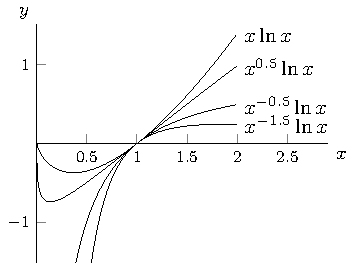
\includegraphics{figEulerCauchyABCD}
\caption*{(ب) دوسری صورت: دوہرا جذر۔}
\end{subfigure}
\begin{subfigure}{0.5\textwidth}
\centering
\begin{tikzpicture}
\begin{axis}[small,axis lines*=middle,ymin=-1.6,ymax=1.6,xmin=0,xmax=2.9,xlabel={$x$},ylabel={$y$},xlabel style={at={(axis description cs:1.05,0.5)}},ylabel style ={rotate=-90},ylabel style={at={(axis description cs:0,1.05)}}]
\addplot[domain=0.001:2,samples=100]{x^(0.1)*cos(180/pi*3*ln(x))}node[below]{$x^{0.1}\cos(3\ln x)$};
\addplot[domain=0.001:2,samples=100]{x^(0.1)*sin(180/pi*3*ln(x))}node[above]{$x^{0.1}\sin(3\ln x)$};
\end{axis}
\end{tikzpicture}
\caption*{(پ) جوڑی دار مخلوط جذر۔}
\end{subfigure}
\caption{یولر کوشی سادہ تفرقی مساوات کے حل۔}
\label{شکل_سادہ_دو_درجی_یولر_کوشی}
\end{figure}

شکل \حوالہ{شکل_سادہ_دو_درجی_یولر_کوشی} میں یولر کوشی سادہ تفرقی مساوات کی تینوں صورتوں کے حل دکھائے گئے ہیں۔

%============================
\ابتدا{مثال}\شناخت{مثال_سادہ_دو_ہم_محوری_نلکی_میدان}\quad دو ہم محوری نلکیوں کے بیچ میں ساکن برقی میدان؛ سرحدی قیمت مسئلہ\\
دو ہم محوری نلکیوں  کے بیچ میں برقی دباو تفرقی مساوات \عددی{\rho \tfrac{\dif^{\,2} v}{\dif \rho^2}+\tfrac{\dif v}{\dif \rho}=0} دیتی ہے۔نلکی کے رداس \عددی{\rho_1=\SI{2}{\centi\meter}} اور \عددی{\rho_2=\SI{5}{\centi\meter}} ہیں جبکہ ان پر \اصطلاح{برقی دباو}\فرہنگ{برقی دباو}\حاشیہب{electric voltage}\فرہنگ{voltage} \عددی{v_1=\SI{50}{\volt}} اور \عددی{v_2=\SI{0}{\volt}} ہے۔درمیانی خطے کی برقی دباو حاصل کریں۔

حل:یولر کوشی مساوات میں \عددی{a=1} اور \عددی{b=0} موجودہ تفرقی مساوات دیتا ہے۔دیے مساوات میں \عددی{v=\rho^m} پر کرتے ہوئے ذیلی مساوات \عددی{m^2=0} حاصل ہوتی ہے جس کا دوہرا جذر \عددی{m=0} ہے۔یوں عمومی  حل \عددی{v=c_1+c_2\ln x} ہو گا۔دیے گئے سرحدی شرائط حل میں پر کرتے 
\begin{align*}
50=c_1+c_2\ln 0.02, \quad 0=c_1+c_2\ln 0.05
\end{align*}
ہوئے \عددی{c_1=-163.471} اور \عددی{c_2=-54.568} حاصل ہوتے ہیں لہٰذا مخصوص حل \عددی{y=-163.471-54.568\ln \rho} ہو گا جسے شکل \حوالہ{شکل_مثال_سادہ_دو_ہم_محوری_نلکی_میدان} میں دکھایا گیا ہے۔
\begin{figure}
\centering
\begin{tikzpicture}
\begin{axis}[small,axis lines*=middle,ymin=0,ymax=58,xmin=0.02,xmax=0.056,xlabel={$\rho$},ylabel={$v$},xlabel style={at={(axis description cs:1.05,0)}},ylabel style ={rotate=-90},ylabel style={at={(axis description cs:0,1.05)}},scaled x ticks=false,xtick={0.02,0.03,0.04,0.05},xticklabels={$2$,$3$,$4$,$5$},ytick={0,50},yticklabels={$0$,$50$}]
\addplot[domain=0.01:0.05]{-163.471-54.568*ln(x)};
\end{axis}
\end{tikzpicture}
\caption{مثال \حوالہ{مثال_سادہ_دو_ہم_محوری_نلکی_میدان} کا حل۔}
\label{شکل_مثال_سادہ_دو_ہم_محوری_نلکی_میدان}
\end{figure}
\انتہا{مثال}
%==========================
\ابتدا{مثال}
یولر کوشی مساوات \حوالہ{مساوات_سادہ_دو_درجی_یولر_کوشی_الف} میں \عددی{x=e^{t}} پر کرتے ہوئے اس کو مستقل عددی سر والے سادہ تفرقی مساوات میں تبدیل کریں۔

حل:ہم \عددی{y(x)} کو \عددی{y[x(t)]} یعنی \عددی{y(t)} تصور کرتے ہیں۔یوں زنجیری تفرق سے
\begin{align*}
\frac{\dif y}{\dif x}=\frac{\dif y}{\dif t}\frac{\dif t}{\dif x}, \quad \frac{\dif^{\,2} y}{\dif x^2}=\frac{\dif^{\,2}y}{\dif t^2}\left(\frac{\dif t}{\dif x}\right)^2+\frac{\dif y}{\dif t}\frac{\dif^{\,2} t}{\dif x^2}
\end{align*}
لکھا جا سکتا ہے۔ان میں \عددی{\tfrac{\dif t}{\dif x}=\tfrac{1}{x}} اور \عددی{\tfrac{\dif^{\,2} t}{\dif x^2}=-\tfrac{1}{x^2}} پر کرتے ہیں۔
\begin{align*}
\frac{\dif y}{\dif x}=\frac{1}{x}\frac{\dif y}{\dif t}, \quad \frac{\dif^{\,2} y}{\dif x^2}=\frac{1}{x^2}\frac{\dif^{\,2}y}{\dif t^2}-\frac{1}{x^2}\frac{\dif y}{\dif t}
\end{align*}
انہیں مساوات \حوالہ{مساوات_سادہ_دو_درجی_یولر_کوشی_الف} میں پر کرتے 
\begin{align*}
x^2\left(\frac{1}{x^2}\frac{\dif^{\,2}y}{\dif t^2}-\frac{1}{x^2}\frac{\dif y}{\dif t}\right)+ax\left(\frac{1}{x}\frac{\dif y}{\dif t}\right)+by=0
\end{align*}
ہوئے مستقل عددی سر والا سادہ تفرقی مساوات حاصل ہوتا ہے  جہاں \عددی{\dot{y}=\tfrac{\dif y}{\dif t}} اور \عددی{\ddot{y}=\tfrac{\dif^{\,2}y}{\dif t^2}} ہیں۔
\begin{align}
\ddot{y}+(a-1)\dot{y}+by=0
\end{align}
\انتہا{مثال}
%==================================

\حصہء{سوالات}
سوال \حوالہ{سوال_سادہ_دو_یولر_کوشی_الف} تا سوال \حوالہ{سوال_سادہ_دو_یولر_کوشی_ب} حل کریں۔
%=======================

\ابتدا{سوال}\شناخت{سوال_سادہ_دو_یولر_کوشی_الف}
\begin{align*}
x^2y''-2xy'+2y=0
\end{align*}
جواب:\عددی{y=c_1x+c_2x^2}
\انتہا{سوال}
%====================
\ابتدا{سوال}
\begin{align*}
x^2y''-6y=0
\end{align*}
جواب:\عددی{y=c_1x^3+c_2x^{-2}}
\انتہا{سوال}
%==========================
\ابتدا{سوال}
\begin{align*}
x^2y''+6xy'+4y=0
\end{align*}
جواب:\عددی{y=\tfrac{c_1}{x}+\tfrac{c_2}{x^4}}
\انتہا{سوال}
%==================
\ابتدا{سوال}
\begin{align*}
x^2y''-5xy'+9y=0
\end{align*}
جواب:\عددی{y=(c_1+c_2\ln x)x^3}
\انتہا{سوال}
%==========================
\ابتدا{سوال}
\begin{align*}
x^2y''+11xy'+25y=0
\end{align*}
جواب:\عددی{y=(c_1+c_2\ln x)x^{-5}}
\انتہا{سوال}
%========================
\ابتدا{سوال}
\begin{align*}
10x^2y''+11xy'-3y=0
\end{align*}
جواب:\عددی{y=c_1\sqrt{x}+c_2x^{-\tfrac{3}{5}}}
\انتہا{سوال}
%=====================
\ابتدا{سوال}
\begin{align*}
x^2y''+0.44xy'+0.0748y=0
\end{align*}
جواب:\عددی{y=c_1x^{0.22}+c_2x^{0.34}}
\انتہا{سوال}
%======================
\ابتدا{سوال}
\begin{align*}
x^2y''+0.4xy'+0.73y=0
\end{align*}
جواب:\عددی{y=x^{0.3}[c_1\cos(0.8\ln x)+c_2\sin(0.8\ln x)]}
\انتہا{سوال}
%===================
\ابتدا{سوال}\شناخت{سوال_سادہ_دو_یولر_کوشی_ب}
\begin{align*}
x^2y''+2xy'+4.25y=0
\end{align*}
جواب:\عددی{y=x^{-0.5}[c_1\cos(2\ln x)+c_2\sin(2\ln x)]}
\انتہا{سوال}
%======================
سوال \حوالہ{سوال_سادہ_دو_یولر_کوشی_پ} تا سوال \حوالہ{سوال_سادہ_دو_یولر_کوشی_ت} ابتدائی قیمت مسئلے ہیں۔انہیں حل کریں۔

\ابتدا{سوال}\شناخت{سوال_سادہ_دو_یولر_کوشی_پ}
\begin{align*}
x^2y''-0.4xy'+0.45y=0,\quad y(1)=2,\quad y'(1)=-1
\end{align*}
جواب:\عددی{y=7\sqrt{x}-5x^{0.9}}
\انتہا{سوال}
%================================
\ابتدا{سوال}
\begin{align*}
x^2y''+1.08xy'-0.01713y=0,\quad y(1)=-1,\quad y'(1)=1
\end{align*}
جواب:\عددی{y=\tfrac{23}{18}x^{0.23}-\tfrac{41}{18}x^{-0.31}}
\انتہا{سوال}
%================================
\ابتدا{سوال}
\begin{align*}
35x^2y''+57xy'+3y=0,\quad y(1)=3,\quad y'(1)=-5
\end{align*}
جواب:\عددی{y=\tfrac{77}{4}x^{-\tfrac{3}{7}}-\tfrac{65}{4}x^{-\tfrac{1}{5}}}
\انتہا{سوال}
%================================
\ابتدا{سوال}
\begin{align*}
6x^2y''+19xy'+6y=0,\quad y(1)=-3,\quad y'(1)=1
\end{align*}
جواب:\عددی{y=\tfrac{6}{5}x^{-\tfrac{3}{2}}-\tfrac{21}{5}x^{-\tfrac{2}{3}}}
\انتہا{سوال}
%================================
\ابتدا{سوال}
\begin{align*}
25x^2y''-15xy'+16y=0,\quad y(2)=0,\quad y'(2)=1
\end{align*}
جواب:\عددی{y=2^{\tfrac{1}{5}}x^{\tfrac{4}{5}}(\ln x-\ln 2)}
\انتہا{سوال}
%================================
\ابتدا{سوال}\شناخت{سوال_سادہ_دو_یولر_کوشی_ت}
\begin{align*}
49x^2y''+77xy'+4y=0,\quad y(2)=3,\quad y'(2)=0
\end{align*}
جواب:\عددی{y=x^{-\tfrac{2}{7}}(2.93+1.04\ln x)}
\انتہا{سوال}
%================================

\حصہ{حل کی وجودیت اور یکتائی؛ ورونسکی}
اس حصے میں متجانس خطی سادہ تفرقی مساوات،
\begin{align}\label{مساوات_سادہ_دو_وجودیت_مخصوص_الف}
y''+p(x)y'+q(x)y=0
\end{align}
جس کے عددی سر \عددی{p(x)} اور \عددی{q(x)} کوئی بھی \اصطلاح{استمراری تفاعل} ہو سکتے  ہیں، کے عمومی حل کی \اصطلاح{وجودیت}\فرہنگ{وجودیت}\حاشیہب{existence}\فرہنگ{existence} پر غور کیا جائے گا۔ساتھ ہی ساتھ مساوات \حوالہ{مساوات_سادہ_دو_وجودیت_مخصوص_الف} اور  ابتدائی معلومات
\begin{align}\label{مساوات_سادہ_دو_وجودیت_مخصوص_ب}
y(x_0)=K_0, \quad y'(x_0)=K_1
\end{align}
کے  ابتدائی قیمت مسئلہ کی مخصوص حل کی \اصطلاح{یکتائی}\فرہنگ{یکتائی}\حاشیہب{uniqueness}\فرہنگ{uniqueness} پر بحث کی جائے گی۔ 

مسئلہ \حوالہ{مسئلہ_سادہ_دو_درجی_یکتا_مخصوص_حل} کہتا ہے کہ اس ابتدائی قیمت مسئلے کا مخصوص حل پایا جاتا ہے جو یکتا ہو گا اور مساوات \حوالہ{مساوات_سادہ_دو_وجودیت_مخصوص_الف} کے عمومی حل
\begin{align}
y=c_1y_1+c_2y_2\quad \quad \text{\RL{اختیاری $c_1$, $c_2$}}
\end{align}
میں تمام حل شامل ہیں۔یوں استمراری عددی سر والے متجانس سادہ تفرقی مساوات کا کوئی \اصطلاح{نادر حل}\فرہنگ{نادر حل}\فرہنگ{حل!نادر} نہیں پایا جاتا۔نادر حل اس حل کو کہتے ہیں جسے عمومی حل سے حاصل نہیں کیا جا سکتا ہے۔

ہمیں مستقل عددی سر والے سادہ تفرقی مساوات یا یولر کوشی سادہ تفرقی مساوات کے حل کی وجودیت اور یکتائی جاننے کی ضرورت پیش نہیں آئی چونکہ ان کے حل کے دوران ہی ایسی تمام معلومات سامنے آ جاتی ہیں۔
%================

%\theoremstyle{plain}
%\begin{theorem}[]\label{مسئلہ_سادہ_دو_درجی_یکتا_مخصوص_حل}
\ابتدا{مسئلہ}\شناخت{مسئلہ_سادہ_دو_درجی_یکتا_مخصوص_حل}\quad مسئلہ وجودیت اور یکتائی برائے ابتدائی قیمت تفرقی مساوات\فرہنگ{مسئلہ!وجودیت اور یکتائی}\\
اگر \عددی{p(x)} اور \عددی{q(x)} کسی کھلے  وقفے \عددی{I} پر استمراری ہوں اور \عددی{x_0} اس وقفے پر پایا جاتا ہو، تب مساوات \حوالہ{مساوات_سادہ_دو_وجودیت_مخصوص_الف} اور مساوات \حوالہ{مساوات_سادہ_دو_وجودیت_مخصوص_ب} پر مبنی ابتدائی قیمت مسئلے کا \عددی{I} پر  یکتا مخصوص حل \عددی{y(x)}  موجود ہے۔  
%\end{theorem}
\انتہا{مسئلہ}
%============================

وجودیت حل کی ثبوت کے لئے وہی بنیادی شرائط درکار ہیں جو صفحہ \حوالہصفحہ{مسئلہ_سادہ_اول_وجودیت} پر مسئلہ \حوالہ{مسئلہ_سادہ_اول_وجودیت} کے لئے درکار تھے۔اس کتاب میں ان پر غور نہیں کیا جائے گا۔ اگرچہ یکتائی کا ثبوت عموماً آسان ہوتا ہے لیکن موجودہ مسئلہ \حوالہ{مسئلہ_سادہ_دو_درجی_یکتا_مخصوص_حل} کے یکتائی حل کا ثبوت اتنا آسان نہیں ہے لہٰذا اس کو کتاب کے آخر میں بطور ضمیمہ \حوالہ{ضمیمہ_اضافی_ثبوت} شامل کیا گیا ہے۔ 
%==================

\جزوحصہء{خطی طور غیر تابع حل}
آپ کو حصہ \حوالہ{حصہ_سادہ_اسپرنگ_کمیت} سے یاد ہو گا کہ کھلے وقفہ \عددی{I} پر عمومی حل \اصطلاح{اساس} \عددی{y_1}، \عددی{y_2} پر مشتمل ہوتا ہے جہاں \عددی{y_1} اور \عددی{y_2} کھلے وقفے \عددی{I} پر خطی طور غیر تابع حل ہیں۔ وقفہ \عددی{I} پر معین \عددی{y_1} اور \عددی{y_2}،  وقفہ \عددی{I}  پر، اس صورت \اصطلاح{خطی طور غیر تابع}\فرہنگ{خطی طور! غیر تابع}\حاشیہب{linearly independent}\فرہنگ{linearly independent} کہلاتے ہیں جب پورے وقفے پر
\begin{align}\label{مساوات_سادہ_دو_خطی_طور_غیر_تابع_الف}
k_1 y_1+k_2 y_2=0
\end{align}
سے مراد 
\begin{align}
k_1=0, \quad k_2=0
\end{align}
ہو۔\عددی{k_1} اور \عددی{k_2} میں سے کم از کم ایک کی قیمت صفر کے برابر نہ ہونے کی صورت میں مساوات \حوالہ{مساوات_سادہ_دو_خطی_طور_غیر_تابع_الف} پر پورا اترتے ہوئے حل \عددی{y_1} اور \عددی{y_2} \اصطلاح{خطی طور تابع}\فرہنگ{خطی طور!تابع}\حاشیہب{linearly dependent}\فرہنگ{linearly dependent} کہلاتے ہیں۔اگر \عددی{k_1 \ne 0} ہو تب ہم مساوات \حوالہ{مساوات_سادہ_دو_خطی_طور_غیر_تابع_الف} کو \عددی{k_1} سے تقسیم کرتے ہوئے \عددی{y_1=-\tfrac{k_2}{k_1}y_2} لکھ سکتے ہیں جو تناسبی رشتہ ہے۔اسی طرح \عددی{k_2 \ne 0} کی صورت میں \عددی{y_2=-\tfrac{k_1}{k_2}y_1} لکھا جا سکتا ہے جو تناسبی رشتے کو ظاہر کرتی ہے۔
\begin{align}\label{مساوات_سادہ_دور_خطی_غیر_تابع_شرط}
\text{(الف)}\quad y_1=ky_2,\quad \text{(ب)}\quad y_2=l y_1 \quad \quad \text{\RL{پورے $I$ پر}}
\end{align}
اس کے برعکس خطی طور غیر تابع صورت میں ہم مساوات \حوالہ{مساوات_سادہ_دو_خطی_طور_غیر_تابع_الف} کو \عددی{k_1} (یا \عددی{k_2}) سے تقسیم نہیں کر سکتے لہٰذا  تناسبی رشتہ حاصل نہیں کیا جا سکتا۔(درج بالا مساوات میں \عددی{k=-\tfrac{k_2}{k_1}} اور \عددی{l=-\tfrac{k_1}{k_2}} لکھے گئے ہیں۔\عددی{k} یا (اور) \عددی{l} صفر بھی ہو سکتے ہیں۔) خطی طور غیر تابع اور خطی طور تابع حل کو درج ذیل طرز پر بیان کیا جا سکتا ہے۔ 
%==========================

%\begin{theorem}[خطی طور تابع اور غیر تابع حل]
\ابتدا{مسئلہ}\شناخت{مسئلہ_سادہ_دو_حل_تابع_غیر_تابع}\quad خطی طور تابع اور غیر تابع حل\فرہنگ{مسئلہ!تابع اور غیر تابع حل}\\
کھلے وقفہ \عددی{I} پر استمراری  \عددی{p(x)} اور \عددی{q(x)} عددی سر والے سادہ تفرقی  مساوات \حوالہ{مساوات_سادہ_دو_خطی_طور_غیر_تابع_الف} کے \عددی{I}  پر دو حل \عددی{y_1} اور \عددی{y_2} اس صورت خطی طور غیر تابع ہوں گے جب ان کے \اصطلاح{ورونسکی}\فرہنگ{ورونسکی}\حاشیہب{Wronskian}\فرہنگ{Wronskian}
\begin{align}\label{مساوات_سادہ_دو_ورونسکی_تعریف}
W(y_1,y_2)=y_1y_2'-y_2y_1'
\end{align}
کی قیمت  کسی \عددی{x_0} پر صفر کے برابر ہو جہاں \عددی{x_0} کھلے وقفے \عددی{I} پر پایا جاتا ہے۔مزید اگر  نقطہ \عددی{x=x_0} پر \عددی{W=0} ہو تب پورے \عددی{I} پر \عددی{W=0} ہو گا۔یوں اگر \عددی{I} پر کوئی ایسا \عددی{x} پایا جاتا ہو جس پر \عددی{W} صفر کے برابر نہ ہو تب \عددی{y_1} اور \عددی{y_2} خطی طور غیر تابع ہوں گے۔
%\end{theorem}
\انتہا{مسئلہ}
%==================
\ابتدا{ثبوت}
\begin{enumerate}
\item[(الف)]
\عددی{y_1} اور \عددی{y_2} کو \عددی{I} پر خطی طور غیر تابع تصور کریں۔یوں مساوات \حوالہ{مساوات_سادہ_دور_خطی_غیر_تابع_شرط}-الف یا ب میں سے ایک درست ہو گا۔اگر  مساوات \حوالہ{مساوات_سادہ_دور_خطی_غیر_تابع_شرط}-الف  درست ہو تب
\begin{align*}
W(y_1,y_2)=y_1y_2'-y_2y_1'=ky_2y_2'-y_2ky_2'=0
\end{align*}
ہو گا۔اسی طرح مساوات \حوالہ{مساوات_سادہ_دور_خطی_غیر_تابع_شرط}-ب کی صورت میں بھی \عددی{W=0} ملتا ہے۔
\item[(ب)]
 اس کے الٹ چلتے ہوئے ہم ثابت کرتے ہیں کہ کسی \عددی{x_0} پر \عددی{W(y_1,y_2)=0} سے مراد \عددی{y_1} اور \عددی{y_2} کا \عددی{I} پر خطی طور تابع ہونا ہے۔درج ذیل مساوات پر غور کریں جہاں \عددی{k_1} اور \عددی{k_2} کو نا معلوم متغیرات تصور کریں۔
\begin{gather}
\begin{aligned}\label{مساوات_سادہ_دو_درجی_ثبوت_الف}
k_1y_1(x_0)+k_2y_2(x_0)&=0\\
k_1y_1'(x_0)+k_2y_2'(x_0)&=0
\end{aligned}
\end{gather}
\عددی{k_2} حذف کرنے کی نیت سے  پہلی مساوات کو \عددی{y_2'(x_0)} اور دوسری کو \عددی{-y_2(x_0)} سے ضرب دیتے ہوئے دونوں کا مجموعہ لیتے ہیں۔
\begin{align}\label{مساوات_سادہ_دو_درجی_ثبوت_ب}
k_1y_1(x_0)y_2'(x_0)-k_1y_1'(x_0)y_2(x_0)=k_1W(y_1(x_0),y_2(x_0))=0
\end{align}
اسی طرح \عددی{k_1} حذف کرنے کے لئے پہلی مساوات کو \عددی{-y_1'(x_0)} اور دوسری کو \عددی{y_1(x_0)} سے ضرب دیتے ہوئے دونوں مساوات کا مجموعہ
\begin{align}\label{مساوات_سادہ_دو_درجی_ثبوت_پ}
k_2y_1(x_0)y_2'(x_0)-k_2y_2(x_0)y_1'(x_0)=k_2W(y_1(x_0),y_2(x_0))=0
\end{align}
لیتے ہیں۔اب اگر \عددی{x_0} پر \عددی{W} صفر نہ ہوتا تب ہم مساوات \حوالہ{مساوات_سادہ_دو_درجی_ثبوت_ب} اور مساوات \حوالہ{مساوات_سادہ_دو_درجی_ثبوت_پ} کو \عددی{W} سے تقسیم کرتے ہوئے \عددی{k_1=k_2=0} حاصل کرتے البتہ \عددی{x_0} پر \عددی{W(y_1(x_0),y_2(x_0))=0} ہے لہٰذا ہم ان مساوات کو \عددی{W} سے  تقسیم نہیں کر سکتے ہیں۔ یوں  ہمزاد مساوات \حوالہ{مساوات_سادہ_دو_درجی_ثبوت_الف} کا حل \عددی{k_1} اور \عددی{k_2} پایا جاتا ہے جہاں \عددی{k_1} اور \عددی{k_2} دونوں غیر صفر ہو سکتے ہیں۔ اب ان اعداد \عددی{k_1} اور \عددی{k_2} کو استعمال کرتے ہوئے تفاعل
\begin{align}
y(x)=k_1y_1(x)+k_2y_2(x)
\end{align}
لیتے ہیں۔چونکہ مساوات \حوالہ{مساوات_سادہ_دو_وجودیت_مخصوص_الف} متجانس خطی ہے لہٰذا  مسئلہ \حوالہ{مسئلہ_دو_درجی_خطی_میل}  (مسئلہ خطی میل) کے تحت  یہ تفاعل بھی مساوات \حوالہ{مساوات_سادہ_دو_وجودیت_مخصوص_الف} کا حل ہو گا۔مساوات \حوالہ{مساوات_سادہ_دو_درجی_ثبوت_الف} سے ظاہر ہے کہ یہ تفاعل ابتدائی معلومات \عددی{y(x_0)=0} اور \عددی{y'(x_0)=0} پر پورا اترتا ہے۔اب تصور کریں کہ مساوات \حوالہ{مساوات_سادہ_دو_وجودیت_مخصوص_الف} کا دوسرا حل جو انہیں  ابتدائی معلومات پر پورا اترتا ہو \عددی{y^*(x)=0} ہے۔اب چونکہ مساوات \حوالہ{مساوات_سادہ_دو_وجودیت_مخصوص_الف} میں \عددی{p(x)} اور \عددی{q(x)} استمراری ہیں لہٰذا مسئلہ \حوالہ{مسئلہ_سادہ_دو_درجی_یکتا_مخصوص_حل} کے تحت اس کا مخصوص حل یکتا ہو گا۔یوں \عددی{y(x)} اور \عددی{y^*(x)} مختلف نہیں ہو سکتے ہیں لہٰذا \عددی{y^*(x)=y(x)=0} یعنی
\begin{align}\label{مساوات_سادہ_دو_درجی_ثبوت_ت}
k_1y_1+k_2y_2\equiv 0\quad \quad \text{\RL{پورے $I$ پر}}
\end{align}
ہو گا۔چونکہ \عددی{k_1} اور \عددی{k_2} میں کم از کم ایک صفر کے برابر نہیں ہے لہٰذا  مساوات \حوالہ{مساوات_سادہ_دو_درجی_ثبوت_ت} کہتا ہے کہ \عددی{I} پر \عددی{y_1} اور \عددی{y_2} خطی طور تابع ہیں۔
\item[(پ)]
ہم مسئلے کا آخری نقطہ ثابت کرتے ہیں۔اگر کھلے وقفے \عددی{I} پر نقطہ \عددی{x_0} پر \عددی{W(x_0)=0} ہو تب ثبوت (ب) کے تحت \عددی{I} پر \عددی{y_1} اور \عددی{y_2} خطی طور تابع ہیں لہٰذا ثبوت (الف) کے تحت \عددی{W \equiv 0} ہو گا۔یوں خطی طور تابع صورت میں ایسا نہیں ہو سکتا ہے کہ \عددی{W(x_1) \ne 0} ہو جہاں \عددی{x_1} کھلے وقفہ \عددی{I} پر پایا جاتا ہے۔اگر ایسا ممکن ہو تب اس سے مراد خطی طور غیر تابع صورت ہو گی جیسا کہ دعویٰ کیا گیا ہے۔ 
\end{enumerate}
\انتہا{ثبوت}
%=================

حساب کی نقطہ نظر سے  مساوات \حوالہ{مساوات_سادہ_دو_ورونسکی_تعریف} سے درج ذیل زیادہ آسان مساوات ہے۔
\begin{align}\label{مساوات_سادہ_دو_آسان_ورونسکی}
W(y_1,y_2)=
\begin{cases}
\left(\frac{y_2}{y_1}\right)^{\!'}y_1^2  &(y_1 \ne 0)\\[0.5em]
-\left(\frac{y_1}{y_2}\right)^{\!'}y_2^2 & (y_2 \ne 0)
\end{cases}
\end{align}
آپ دیکھ سکتے ہیں کہ  ورونسکی کو قالب کی مقطع کے طرز پر لکھا جا سکتا ہے جس کو \اصطلاح{ورونسکی مقطع}\فرہنگ{ورونسکی!مقطع}\فرہنگ{مقطع!ورونسکی}\حاشیہب{Wronskian determinant}\فرہنگ{Wronskian determinant} یا حل \عددی{y_1} اور \عددی{y_2} کی \اصطلاح{ورونسکی} کہتے ہیں۔ 
\begin{align}
W(y_1,y_2)=
\begin{vmatrix}
y_1 &y_2\\[0.25em]
y_1' & y_2'
\end{vmatrix}
=y_1y_2'-y_2y_1'
\end{align}
%==============================

\ابتدا{مثال}\quad مسئلہ \حوالہ{مسئلہ_سادہ_دو_حل_تابع_غیر_تابع} کا اطلاق\\
تفرقی مساوات \عددی{y''+\omega^2y=0} کے حل \عددی{y_1=\cos \omega x} اور \عددی{y_2=\sin \omega x}  ہیں۔ان کی ورونسکی
\begin{align*}
W(\cos \omega x,\sin \omega x)=
\begin{vmatrix}
\cos \omega x &\sin \omega x\\[0.25em]
-\omega \sin \omega x & -\omega \cos \omega x
\end{vmatrix}
=\omega \cos^2 \omega x+\omega \sin^2 \omega x=\omega
\end{align*}
ہے۔مسئلہ \حوالہ{مسئلہ_سادہ_دو_حل_تابع_غیر_تابع} کے تحت یہ حل صرف اس صورت میں خطی طور غیر تابع ہوں گے جب \عددی{\omega \ne 0} ہو۔یہی دونوں حل کے حاصل تقسیم \عددی{\tfrac{y_2}{y_1}=\tan \omega x} سے بھی اخذ کیا جا سکتا ہے جہاں \عددی{\omega=0} سے \عددیء{y_2=0} ملتا ہے جو خطی طور تابع صورت ظاہر کرتی ہے۔
\انتہا{مثال}
%=============================
\ابتدا{مثال}\quad دوہرا جذر کی صورت میں مسئلہ \حوالہ{مسئلہ_سادہ_دو_حل_تابع_غیر_تابع} کا اطلاق\\
تفرقی مساوات \عددی{y''-6y'+9y=0} کا (ثابت کریں کہ) عمومی حل  \عددی{y=(c_1+c_2 x)e^{3x}}   ہے جس کا ورونسکی صفر کے برابر نہیں ہے لہٰذا \عددی{e^{3x}} اور \عددی{xe^{3x}} تمام \عددی{x} پر خطی طور غیر تابع ہیں۔
\begin{align*}
W(e^{3x},xe^{3x})=
\begin{vmatrix}
e^{3x}& xe^{3x}\\[0.25em]
3e^{3x}&e^{3x}+3xe^{3x}
\end{vmatrix}
=e^{6x}+3xe^{6x}-3xe^{6x}=e^{6x} \ne 0
\end{align*}
\انتہا{مثال}
%==================

\جزوحصہء{مساوات \حوالہ{مساوات_سادہ_دو_وجودیت_مخصوص_الف} کے عمومی حل میں تمام حل کی شمولیت}
اس حصے کو مساوات \حوالہ{مساوات_سادہ_دو_وجودیت_مخصوص_الف} کے عمومی حل کی وجودیت سے شروع کرتے ہیں۔
%=========================

\ابتدا{مسئلہ}\شناخت{مسئلہ_سادہ_دو_وجودیت_الف}\quad \اصطلاح{وجودیت عمومی حل}\فرہنگ{وجودیت!عمومی حل}\فرہنگ{حل!وجودیت عمومی حل}\فرہنگ{existence!solution}\فرہنگ{مسئلہ!وجودیت عمومی حل}\\
کھلے وقفہ \عددی{I} پر استمراری \عددی{p(x)} اور \عددی{q(x)} کی صورت میں مساوات \حوالہ{مساوات_سادہ_دو_وجودیت_مخصوص_الف} کا عمومی حل \عددی{I} پر موجود ہے۔
\انتہا{مسئلہ}
%=====================

\ابتدا{ثبوت}
مسئلہ \حوالہ{مسئلہ_سادہ_دو_درجی_یکتا_مخصوص_حل} کے تحت  \عددی{I} پر مساوات \حوالہ{مساوات_سادہ_دو_وجودیت_مخصوص_الف} کا، ابتدائی معلومات 
\begin{align*}
y_1(x_0)=1, \quad y_1'(x_0)=0
\end{align*}
پر پورا اترتا ہوا  حل  \عددی{y_1(x)} موجود ہے۔اسی طرح ابتدائی معلومات
\begin{align*}
y_2(x_0)=0, \quad y_2'(x_0)=1
\end{align*}
 پر پورا اترتا ہوا  حل \عددی{y_2(x)} بھی موجود ہے۔نقطہ \عددی{x_0} پر ان کا ورونسکی
\begin{align*}
W(y_1(x_0),y_2(x_0))=y_1(x_0)y'_2(x_0)-y_2(x_0)y'_1(x_0)=1
\end{align*}
ہے۔مسئلہ \حوالہ{مسئلہ_سادہ_دو_حل_تابع_غیر_تابع} کے تحت \عددی{I} پر \عددی{y_1} اور \عددی{y_2} خطی طور غیر تابع ہیں لہٰذا یہ مساوات \حوالہ{مساوات_سادہ_دو_وجودیت_مخصوص_الف} کے حل کی اساس ہیں۔اس طرح ثابت ہوا کہ  \عددی{I} پر  مساوات \حوالہ{مساوات_سادہ_دو_وجودیت_مخصوص_الف} کا عمومی حل \عددی{y=c_1y_1+c_2y_2} ہے جہاں \عددی{c_1} اور \عددی{c_2} اختیاری مستقل ہیں۔
\انتہا{ثبوت}
%=======================

آئیں اب ثابت کریں کہ عمومی حل اتنا عمومی ہے جتنا کوئی حل عمومی ہو سکتا ہے۔
%=====================

\ابتدا{مسئلہ}\quad عمومی حل میں تمام حل شامل ہیں\\
کھلا وقفہ \عددی{I} پر استمراری \عددی{p(x)} اور \عددی{q(x)} کی صورت میں \عددی{I} پر مساوات \حوالہ{مساوات_سادہ_دو_وجودیت_مخصوص_الف} کے ہر حل
 \عددی{y=Y(x)} کو
\begin{align}
Y(x)=C_1y_1+C_2y_2
\end{align}
لکھا جا سکتا ہے، جہاں \عددی{y_1} اور \عددی{y_2} کھلے وقفہ \عددی{I} پر مساوات \حوالہ{مساوات_سادہ_دو_وجودیت_مخصوص_الف} کی کوئی بھی اساس اور \عددی{C_1}، \عددی{C_2} مناسب مستقل ہیں۔

یوں مساوات \حوالہ{مساوات_سادہ_دو_وجودیت_مخصوص_الف} کا کوئی \اصطلاح{نادر حل}\فرہنگ{نادر حل} موجود نہیں ہے۔(نادر حل سے مراد ایسا حل ہے جس کو عمومی حل سے حاصل نہیں کیا جا سکتا ہے۔)
\انتہا{مسئلہ}
%======================

\ابتدا{ثبوت}
تصور کریں کہ \عددی{I} پر مساوات \حوالہ{مساوات_سادہ_دو_وجودیت_مخصوص_الف} کا  \عددی{y=Y(x)} کوئی حل ہے۔اب مسئلہ \حوالہ{مسئلہ_سادہ_دو_وجودیت_الف} کے تحت \عددی{I} پر  تفرقی مساوات \حوالہ{مساوات_سادہ_دو_وجودیت_مخصوص_الف} کا عمومی حل
\begin{align}\label{مساوات_سادہ_دو_ثبوت_مسئلہ_چار_الف}
y(x)=c_1y_1(x)+c_2y_2(x)
\end{align}
موجود ہے۔ہم \عددی{c_1} اور \عددی{c_2} کی وہ قیمتیں دریافت کرنا چاہتے ہیں جن سے \عددی{I} پر  \عددی{y(x)=Y(x)} حاصل ہوتا ہو۔ہم \عددی{I} پر کوئی بھی \عددی{x_0} چنتے ہوئے پہلے ثابت کرتے ہیں کہ \عددی{c_1} اور \عددی{c_2} کی ایسی قیمتیں دریافت کی جا سکتی ہیں کہ \عددی{x_0} پر \عددی{y(x_0)=Y(x_0)} اور 
\عددی{y'(x_0)=Y'(x_0)} ہوں۔اس کو مساوات \حوالہ{مساوات_سادہ_دو_ثبوت_مسئلہ_چار_الف} کے استعمال سے 
\begin{align}
c_1y_1(x_0)+c_2y_2(x_0)&=Y(x_0)\label{مساوات_سادہ_دو_ثبوت_مسئلہ_چار_ب}\\
c_1y'_1(x_0)+c_2y'_2(x_0)&=Y'(x_0)\label{مساوات_سادہ_دو_ثبوت_مسئلہ_چار_پ}
\end{align}
لکھ سکتے ہیں۔ان ہمزاد مساوات سے \عددی{c_1} اور \عددی{c_2} معلوم کرتے ہیں۔مساوات \حوالہ{مساوات_سادہ_دو_ثبوت_مسئلہ_چار_ب} کو \عددی{y'_2(x_0)} اور مساوات \حوالہ{مساوات_سادہ_دو_ثبوت_مسئلہ_چار_پ} کو \عددی{-y_2(x_0)} سے ضرب دیتے ہوئے مجموعہ لینے سے \عددی{c_1} حاصل کیا جا سکتا ہے۔ایسا کرنے سے مساوات \حوالہ{مساوات_سادہ_دو_ثبوت_مسئلہ_چار_ت} ملتی ہے۔اسی طرح \عددی{c_2} حاصل کرنے کی خاطر پہلی مساوات کو \عددی{-y'_1(x_0)} اور دوسری کو \عددی{y_1(x_0)} سے ضرب دیتے ہوئے مجموعہ لیتے ہوئے مساوات \حوالہ{مساوات_سادہ_دو_ثبوت_مسئلہ_چار_ٹ} حاصل ہوتی ہے۔ان مساوات میں \عددی{y_1}، \عددی{y'_1}، \عددی{y_2}،\عددی{y'_2}، \عددی{Y} اور \عددی{Y'} کی قیمتیں نقطہ \عددی{x_0} پر لی گئی ہیں۔ 
\begin{align}
c_1y_1y'_2-c_1y_2y'_1&=c_1W(y_1,y_2)=Yy_2'-y_2Y\label{مساوات_سادہ_دو_ثبوت_مسئلہ_چار_ت}\\
c_2y_1y'_2-c_2y_2y'_1&=c_2W(y_1,y_2)=y_1Y-Yy'_1\label{مساوات_سادہ_دو_ثبوت_مسئلہ_چار_ٹ}
\end{align}
اب چونکہ \عددی{y_1} اور \عددی{y_2} حل کی اساس ہیں لہٰذا ورونسکی کی قیمت صفر کے برابر نہیں ہے لہٰذا ان مساوات سے \عددی{c_1} اور \عددی{c_2} حاصل کیے جا سکتے ہیں
\begin{align*}
c_1=\frac{Yy_2'-y_2Y}{W}=C_1, \quad c_2=\frac{y_1Y-Yy'_1}{W}=C_2
\end{align*}
جہاں ان منفرد قیمتوں کو \عددی{C_1} اور \عددی{C_2} لکھا گیا ہے۔ انہیں مساوات \حوالہ{مساوات_سادہ_دو_ثبوت_مسئلہ_چار_الف} میں پر کرتے ہوئے مخصوص حل
\begin{align*}
y^*(x)=C_1y_1(x)+C_2y_2(x)
\end{align*}
حاصل ہوتا ہے۔اب چونکہ \عددی{C_1} اور \عددی{C_2} مساوات \حوالہ{مساوات_سادہ_دو_ثبوت_مسئلہ_چار_ب} اور مساوات \حوالہ{مساوات_سادہ_دو_ثبوت_مسئلہ_چار_پ} کے حل ہیں لہٰذا ہم ان مساوات سے دیکھتے ہیں کہ
\begin{align*}
y^{*}(x_0)=Y(x_0),\quad y^{*'}(x_0)=Y'(x_0)
\end{align*}
مسئلہ \حوالہ{مسئلہ_سادہ_دو_درجی_یکتا_مخصوص_حل} میں جس یکتائی کا ذکر کیا گیا ہے اس کے تحت \عددی{y^*} اور \عددی{Y} تمام \عددی{I} پر ہر جگہ برابر ہوں گے۔
\انتہا{ثبوت}
%=========================

\حصہء{سوالات}
%===================

\ابتدا{سوال}
مساوات \حوالہ{مساوات_سادہ_دو_آسان_ورونسکی} سے مساوات \حوالہ{مساوات_سادہ_دو_ورونسکی_تعریف} حاصل کریں۔
\انتہا{سوال}
%===========================
سوال \حوالہ{سوال_سادہ_ورونسکی_الف} تا سوال \حوالہ{سوال_سادہ_ورونسکی_ب} کی ورونسکی حاصل کریں۔حاصل تقسیم سے ثابت کریں کہ یہ خطی طور غیر تابع ہیں اور مسئلہ \حوالہ{مسئلہ_سادہ_دو_حل_تابع_غیر_تابع} سے  بھی اس بات کی تصدیق کریں

%======================
\ابتدا{سوال}\شناخت{سوال_سادہ_ورونسکی_الف}\quad $e^{2x}, e^{-1.2x}$\\
جوابات:\عددی{\tfrac{e^{2x}}{e^{-1.2x}}=e^{3.2x} \ne c}، \عددی{W=-3.2e^{0.8x}\ne 0}
\انتہا{سوال}
%============================ 
\ابتدا{سوال}\quad $e^{2.4x}, e^{1.1x}$\\
جوابات:\عددی{\tfrac{y_1}{y_2}=e^{1.3x} \ne c}، \عددی{W=-1.3e^{3.5x} \ne 0}
\انتہا{سوال}
%===============
\ابتدا{سوال}\quad
$x, \frac{1}{x}$\\
جوابات:\عددی{\tfrac{y_1}{y_2}=x^2 \ne c}، \عددی{W=-2x^{-2} \ne 0}
\انتہا{سوال}
%=====================
\ابتدا{سوال}\quad
$x, x^3$\\
جوابات:\عددی{\tfrac{y_1}{y_2}=x^{-2} \ne c}، \عددی{W=2x^3 \ne 0}
\انتہا{سوال}
%===================
\ابتدا{سوال}\quad
$e^{-0.2x}\sin 3x, e^{-0.2x} \cos 3x$\\
جوابات:\عددی{\tfrac{y_1}{y_2}=\tan 3x \ne c}، \عددی{W=3e^{-0.4x} \ne 0}
\انتہا{سوال}
%========================
\ابتدا{سوال}\quad
$e^{-ax}\sinh kx, e^{-ax} \cosh kx$\\
جوابات:\عددی{\tfrac{y_1}{y_2}=\tanh kx \ne c}، \عددی{W=-ke^{-2ax} \ne 0}
\انتہا{سوال}
%============================
\ابتدا{سوال}\شناخت{سوال_سادہ_ورونسکی_ب}\quad
$x^{a}\sin(k\ln x), x^{a}\cos(k\ln x)$\\
جوابات:\عددی{\tfrac{y_1}{y_2}=\tan(k \ln x) \ne c}، \عددی{W=-kx^{2a-1} \ne 0}
\انتہا{سوال}
%===========================

سوال \حوالہ{سوال_سادہ_ورونسکی_پ} تا سوال \حوالہ{سوال_سادہ_ورونسکی_ت} میں تفرقی مساوات کے حل دیے گئے ہیں۔تفرقی مساوات حاصل کریں۔ورونسکی کی مدد سے ثابت کریں کہ دیے گئے حل خطی طور غیر تابع ہیں اور ابتدائی قیمت مسئلے کا مخصوص حل حاصل کریں۔
%==============================

\ابتدا{سوال}\شناخت{سوال_سادہ_ورونسکی_پ}\quad 
$\sin 3x, \, \cos 3x,\quad y(0)=2,\quad y'(0)=-3 $\\
جوابات:\عددی{y''+9y=0}، \عددی{W=-3\ne 0}، \عددی{y=2\cos 3x-\sin 3x}
\انتہا{سوال}
%===========================
\ابتدا{سوال}\quad 
$x^3, \, x^{-4},\quad y(1)=-1,\quad y'(1)=2 $\\
جوابات:\عددی{x^2y''+2xy'-12y=0}، \عددی{W=-\tfrac{7}{x^2}\ne 0}، \عددی{y=-\tfrac{2x^3}{7}-\tfrac{5x^{-4}}{7}}
\انتہا{سوال}
%===========================
\ابتدا{سوال}\quad 
$e^{-1.2x}\sin 0.8x, \, e^{-1.2x}\cos 0.8 x,\quad y(0)=5,\quad y'(0)=7 $\\
جوابات:\عددی{y''+2.4y'+2.08y=0}، \عددی{W=-0.8e^{-2.4x} \ne 0}، \\
\عددی{y=e^{-\tfrac{6}{5}x}(\tfrac{65}{4}\sin\tfrac{4x}{5}+5\cos\tfrac{4x}{5})}
\انتہا{سوال}
%===========================
\ابتدا{سوال}\quad 
$x^3,\, x^3\ln x,\quad y(1)=2,\quad y'(1)=8 $\\
جوابات:\عددی{x^2y''-5xy'+9y=0}، \عددی{W=x^5 \ne 0}، \عددی{y=2x^3(1+\ln x)}
\انتہا{سوال}
%===========================
\ابتدا{سوال}\quad 
$1,\, e^{3x},\quad y(0)=1.5,\quad y'(0)=-2.5 $\\
جوابات:\عددی{y''-3y'=0}، \عددی{W=3e^{3x} \ne 0}، \عددی{y=\tfrac{8}{3}e^{3x}-\tfrac{2}{3}}
\انتہا{سوال}
%===========================
\ابتدا{سوال}\quad 
$e^{-kx}\sin \pi x, \, e^{-kx}\cos \pi x,\quad y(0)=1,\quad y'(0)=-k-\pi $\\
جوابات:\عددی{y''+2ky'+(k^2+\pi^2)y=0}، \عددی{W=-\pi e^{-2kx} \ne 0}، \\
\عددی{y=e^{-kx}(\sin \pi x-\cos \pi x)}
\انتہا{سوال}
%===========================
\ابتدا{سوال}\شناخت{سوال_سادہ_ورونسکی_ت}\quad 
$\sinh 1.8x, \,\cosh 1.8x,\quad y(0)=14.2,\quad y'(0)=16.38 $\\
جوابات:\عددی{y''-3.24y=0}، \عددی{W=-1.8 \ne 0}، \\
\عددی{y=9.1\sinh 1.8x+14.2\cosh 1.8x}
\انتہا{سوال}
%===========================
\ابتدا{سوال}
تفرقی مساوات \عددی{y''-y=0} کا عمومی حل قوت نمائی تفاعل اور \اصطلاح{بذلولی}\فرہنگ{بذلولی}\حاشیہب{hyperbolic}\فرہنگ{hyperbolic!function} تفاعل کی صورت میں لکھیں۔دونوں صورتوں کے مستقل کا تعلق کیا ہے؟

جوابات:\عددی{y=c_1e^{x}+c_2e^{-x}}، \عددی{y=c_a\sinh x+c_b\cosh x}، \عددی{c_a=c_1-c_2}، \عددی{c_b=c_1+c_2}
\انتہا{سوال}
%=============================
%=====================================

\حصہ{غیر متجانس سادہ تفرقی مساوات}\شناخت{حصہ_سادہ_دو_غیر_متجانس}
اس باب میں اب تک متجانس خطی سادہ تفرقی مساوات پر غور کیا گیا۔یہاں سے باب کے اختتام تک غیر متجانس خطی سادہ تفرقی مساوات پر غور کیا جائے گا۔درج ذیل غیر متجانس خطی تفرقی مساوات پر غور کرتے ہیں جہاں \عددی{r \not \equiv 0} ہے۔
\begin{align}\label{مساوات_سادہ_دو_غیر_متجانس_الف}
y''+p(x)y'+q(x)y=r(x)
\end{align}
ہم دیکھیں گے کہ مساوات \حوالہ{مساوات_سادہ_دو_غیر_متجانس_الف} کا عمومی حل، مطابقتی متجانس مساوات 
\begin{align}\label{مساوات_سادہ_دو_غیر_متجانس_ب}
y''+p(x)y'+q(x)y=0
\end{align}
کے عمومی حل اور مساوات \حوالہ{مساوات_سادہ_دو_غیر_متجانس_ب} کے ایک مخصوص حل کا مجموعہ ہو گا۔ مساوات \حوالہ{مساوات_سادہ_دو_غیر_متجانس_الف} کے عمومی حل اور مخصوص حل کی تعریف درج ذیل ہے۔
%==============

\ابتدا{تعریف}\quad عمومی حل اور مخصوص حل\\
کھلے وقفہ \عددی{I} پر غیر متجانس  مساوات \حوالہ{مساوات_سادہ_دو_غیر_متجانس_الف} کا عمومی حل
\begin{align}\label{مساوات_سادہ_دو_غیر_متجانس_پ}
y(x)=y_h(x)+y_p(x)
\end{align}
ہو گا جہاں \عددی{I} پر \عددی{y_h=c_1y_1+c_2y_2} متجانس مساوات \حوالہ{مساوات_سادہ_دو_غیر_متجانس_ب} کا عمومی حل ہے اور \عددی{I} پر \عددی{y_p} مساوات \حوالہ{مساوات_سادہ_دو_غیر_متجانس_الف} کا کوئی بھی حل ہے جس میں مستقل نہیں پایا جاتا۔

مساوات \حوالہ{مساوات_سادہ_دو_غیر_متجانس_الف} کا مخصوص حل، مساوات \حوالہ{مساوات_سادہ_دو_غیر_متجانس_پ} کے  \عددی{c_1} اور \عددی{c_2} میں خصوصی قیمتیں پر کرتے ہوئے حاصل کیا جاتا ہے۔
\انتہا{تعریف}
%=========================

اب ہمیں حل کی ان تعریف کا جواز پیش کرنا ہو گا اور ساتھ ہی ساتھ مساوات \حوالہ{مساوات_سادہ_دو_غیر_متجانس_الف} کا  حل \عددی{y_p} حاصل کرنا ہو گا۔پس ہم پہلے ثابت کرتے ہیں کہ مساوات \حوالہ{مساوات_سادہ_دو_غیر_متجانس_پ} کا عمومی حل مساوات \حوالہ{مساوات_سادہ_دو_غیر_متجانس_الف} پر پورا اترتا ہے اور یہ کہ مساوات \حوالہ{مساوات_سادہ_دو_غیر_متجانس_الف} اور مساوات \حوالہ{مساوات_سادہ_دو_غیر_متجانس_ب} کے حل کا آپس میں سادہ تعلق ہے۔
%=================

\ابتدا{مسئلہ}\شناخت{مسئلہ_سادہ_دو_حل_تعلق}\quad مساوات \حوالہ{مساوات_سادہ_دو_غیر_متجانس_الف} اور مساوات \حوالہ{مساوات_سادہ_دو_غیر_متجانس_ب} کے حل کا آپس میں تعلق\\
\begin{enumerate}
\item[(الف)]
کھلے وقفہ \عددی{I} پر مساوات \حوالہ{مساوات_سادہ_دو_غیر_متجانس_الف} کے حل \عددی{y} اور اسی وقفے پر مساوات \حوالہ{مساوات_سادہ_دو_غیر_متجانس_ب} کے حل \عددیء{\tilde{y}} کا مجموعہ \عددی{I} پر مساوات \حوالہ{مساوات_سادہ_دو_غیر_متجانس_الف} کا حل ہے۔بالخصوص مساوات \حوالہ{مساوات_سادہ_دو_غیر_متجانس_پ} کھلے وقفہ \عددی{I} پر مساوات \حوالہ{مساوات_سادہ_دو_غیر_متجانس_الف} کا حل ہو گا۔
\item[(ب)]
کھلے وقفہ \عددی{ِI} پر مساوات \حوالہ{مساوات_سادہ_دو_غیر_متجانس_الف} کے دو حل کا فرق \عددی{I} پر مساوات \حوالہ{مساوات_سادہ_دو_غیر_متجانس_ب} کا حل ہے۔ 
\end{enumerate}
\انتہا{مسئلہ}
%======================

\ابتدا{ثبوت}
\begin{enumerate}
\item[(الف)]
مساوات \حوالہ{مساوات_سادہ_دو_غیر_متجانس_الف} کے بائیں ہاتھ کو \عددی{L[y]} سے ظاہر کرتے ہیں۔یوں  \عددی{I} پر مساوات \حوالہ{مساوات_سادہ_دو_غیر_متجانس_الف} کے کسی بھی حل \عددی{y} اور مساوات \حوالہ{مساوات_سادہ_دو_غیر_متجانس_ب} کے کسی بھی حل \عددی{\tilde{y}} کے لئے درج ذیل لکھا جا سکتا ہے۔
\begin{align*}
L[y+\tilde{y}]=L[y]+L[\tilde{y}]=r+0=r
\end{align*}
\item[(ب)]
کھلے وقفے \عددی{I} پر مساوات \حوالہ{مساوات_سادہ_دو_غیر_متجانس_الف} کے کسی بھی حل \عددی{y} اور \عددی{y^*} کے لئے درج ذیل لکھا جا سکتا ہے۔
\begin{align*}
L[y-y^*]=L[y]-L[y^*]=r-r=0
\end{align*}
\end{enumerate}
\انتہا{ثبوت}
%=======================

ہم جانتے ہیں کہ متجانس مساوات \حوالہ{مساوات_سادہ_دو_غیر_متجانس_ب} کے عمومی حل میں تمام حل شامل ہوتے ہیں۔اب ہم ثابت کرتے ہیں کہ غیر متجانس مساوات \حوالہ{مساوات_سادہ_دو_غیر_متجانس_الف} کے عمومی حل میں اس کے تمام حل شامل ہیں۔
%===================

\ابتدا{مسئلہ}\quad غیر متجانس سادہ تفرقی مساوات کے عمومی حل میں تمام حل شامل ہیں\\
کھلے وقفہ \عددی{I} پر استمراری \عددی{p(x)}، \عددی{q(x)} اور \عددی{r(x)} کی صورت میں \عددی{I} پر مساوات \حوالہ{مساوات_سادہ_دو_غیر_متجانس_الف} کا ہر حل،  مساوات \حوالہ{مساوات_سادہ_دو_غیر_متجانس_پ} میں دیے گئے عمومی حل کے اختیاری مستقل \عددی{c_1} اور \عددی{c_2} میں موزوں قیمتیں پر کرنے سے حاصل کیا جاتا ہے۔ 
\انتہا{مسئلہ}
%=====================

\ابتدا{ثبوت}
کھلے وقفے \عددی{I} پر \عددی{y^*} مساوات \حوالہ{مساوات_سادہ_دو_غیر_متجانس_الف} کا کوئی حل ہے جبکہ \عددی{x_0} اس وقفے پر کوئی \عددی{x} ہے۔اسی طرح مساوات \حوالہ{مساوات_سادہ_دو_غیر_متجانس_پ} کھلے وقفے پر مساوات \حوالہ{مساوات_سادہ_دو_غیر_متجانس_الف} کا کوئی عمومی حل ہے۔یہ حل موجود ہے۔یقیناً \عددی{y_h=c_1y_1+c_2y_2} مسئلہ \حوالہ{مسئلہ_سادہ_دو_وجودیت_الف} کے تحت موجود ہے جبکہ \عددی{y_p} کی وجودیت اس باب میں آگے جا کر  دکھائی جائے گی۔اب مسئلہ \حوالہ{مسئلہ_سادہ_دو_حل_تعلق}-ب کے تحت  \عددی{Y=y^*-y_p} کھلے وقفے پر مساوات \حوالہ{مساوات_سادہ_دو_غیر_متجانس_ب} کا حل ہے۔نقطہ \عددی{x_0} پر
\begin{align*}
Y(x_0)=y^*(x_0)-y_p(x_0), \quad Y'(x_0)=y^{*'}(x_0)-y_p'(x_0)
\end{align*}
لکھا جا سکتا ہے۔کھلے وقفے  \عددی{I} پر، مسئلہ \حوالہ{مسئلہ_سادہ_دو_درجی_یکتا_مخصوص_حل} کے مطابق، کسی بھی ابتدائی معلومات کی طرح، ان معلومات پر پورا اترتا ہوا، مساوات \حوالہ{مساوات_سادہ_دو_غیر_متجانس_ب} کا مخصوص حل موجود ہے جسے \عددی{y_h} میں \عددی{c_1} اور \عددی{c_2} میں موزوں  قیمتیں پر کرنے سے حاصل کیا جا سکتا ہے۔  اس حقیقت کو مد نظر رکھتے ہوئے  \عددی{y^*=Y+y_p} سے مسئلہ کا دعویٰ ثابت ہوتا ہے۔
\انتہا{ثبوت}
%======================
%========================
\جزوحصہء{نا معلوم عددی سر کی ترکیب}
آپ نے دیکھا کہ مساوات \حوالہ{مساوات_سادہ_دو_غیر_متجانس_الف} یا اس پر مبنی ابتدائی قیمت مسئلے کا حل  حاصل کرنے کی خاطر مساوات \حوالہ{مساوات_سادہ_دو_غیر_متجانس_ب} کو حل کرنا ہو گا اور مساوات \حوالہ{مساوات_سادہ_دو_غیر_متجانس_الف} کا کوئی بھی حل \عددی{y_p}  تلاش کرنا ہو گا۔اس طرح عمومی حل \حوالہ{مساوات_سادہ_دو_غیر_متجانس_پ} حاصل ہو گا۔

مساوات \حوالہ{مساوات_سادہ_دو_غیر_متجانس_الف} کا حل \عددی{y_p} حاصل کرنے کی ایک ترکیب کو \اصطلاح{نا معلوم عددی سر کی ترکیب}\فرہنگ{نا معلوم عددی سر!ترکیب}\حاشیہب{method of undetermined coefficients}\فرہنگ{coefficients!undetermined method}  کہتے ہیں۔یہ ترکیب نہایت آسان ہے۔ اس ترکیب سے ارتعاشی نظام عمدگی سے حل ہوتے ہیں لہٰذا اسے انجینئری شعبے میں مقبولیت حاصل ہے۔اس باب کے آخری حصے میں عمومی ترکیب پر غور کیا جائے گا جو نسبتاً مشکل ترکیب ہے۔

نا معلوم عددی سر کی ترکیب ان خطی سادہ تفرقی مساوات
\begin{align}\label{مساوات_سادہ_دو_نا_معلوم_الف}
y''+ay'+by=r(x)
\end{align}
 کے حل کے لئے موزوں ہے جس کے عددی سر \عددی{a} اور \عددی{b} مستقل مقدار ہوں اور \عددی{r(x)} قوت نمائی تفاعل ہو یا \عددی{x} کی طاقت ہو یا  سائن نما تفاعل ہو اور یا ان تفاعل کا مجموعہ یا حاصل ضرب ہو۔ایسی تفاعل کی تفرقات بھی یہی تفاعل ہوتی ہیں۔مثلاً \عددی{x^3} کے تفرقات   \عددی{3x^2}، \عددی{6x} اور \عددی{6} ہیں جو از خود \عددی{x} کی طاقت ہیں۔اسی طرح \عددی{\sin \omega x} کا ایک درجی تفرق \عددی{\omega \cos \omega x} جبکہ دو درجی تفرق \عددی{-\omega^2\sin\omega x} ہے۔یہ دونوں تفرقات از خود  سائن نما تفاعل ہیں۔

اس ترکیب میں \عددی{y_p} کو \عددی{r(x)} اور اس کے تمام تفرقات کے مجموعے کی صورت میں  لکھا جاتا ہے۔مجموعہ لکھتے ہوئے ہر رکن کو نا معلوم مستقل سے ضرب دیا جاتا ہے۔ \عددی{y_p} اور اس کے تفرقات کو  مساوات \حوالہ{مساوات_سادہ_دو_نا_معلوم_الف} میں پر کرتے ہوئے دونوں اطراف کے یکساں اجزاء کے عددی سر برابر لکھتے ہوئے نا معلوم مستقل دریافت کئے جاتے ہیں۔تفاعل \عددی{r(x)} سے \عددی{y_p} جدول \حوالہ{جدول_سادہ_دو_نا_معلوم_عددی_سر} کے تحت لکھی جاتی ہے۔تفاعل \عددی{r(x)} سے \عددی{y_p}  درج ذیل قواعد کے تحت لکھی جاتی ہے۔
\begin{enumerate}
\item[بنیادی قاعدہ:]
اگر مساوات \حوالہ{مساوات_سادہ_دو_نا_معلوم_الف} کا \عددی{r(x)} جدول  \حوالہ{جدول_سادہ_دو_نا_معلوم_عددی_سر} کے دائیں قطار میں دیا گیا ہو تب اس تفاعل کے صف سے \عددی{y_p(x)} حاصل کریں۔حاصل \عددی{y_p} اور اس کے تفرقات کو مساوات \حوالہ{جدول_سادہ_دو_نا_معلوم_عددی_سر} میں پر کرتے ہوئے نا معلوم عددی سر کی قیمت دریافت کریں۔ 
\item[ترمیمی قاعدہ:]
اگر \عددی{y_p}  کا کوئی رکن تفاعل مساوات \حوالہ{مساوات_سادہ_دو_نا_معلوم_الف} کے  مطابقتی متجانس مساوات کا حل ہو تب  اس رکن کو \عددی{x} سے ضرب دے کر \عددی{y_p} میں شامل کریں۔(اگر یہ حل مطابقتی متجانس مساوات کے امتیازی مساوات کے دوہرے جذر  سے حاصل کیا گیا ہو تب اس رکن کو \عددی{x^2} سے ضرب دیں۔)  
\item[مجموعے کا قاعدہ:]
اگر \عددی{r(x)} جدول \حوالہ{جدول_سادہ_دو_نا_معلوم_عددی_سر} کے دائیں قطار میں پائے جانے والے تفاعل کا مجموعہ ہو تب \عددی{y_p} کو ان تفاعل کے صف میں بائیں قطار کے تفاعل کا مجموعہ لکھیں۔
\end{enumerate} 
%======================================

\عددی{r(x)} صرف ایک رکن پر مشتمل ہونے کی صورت میں بنیادی قاعدہ استعمال ہو گا۔ترمیمی قاعدہ استعمال کرنے سے پہلے متجانس مساوات حل کرنا ہو گا۔اگر \عددی{r=r_1} کی صورت میں مساوات \حوالہ{مساوات_سادہ_دو_نا_معلوم_الف} کا حل \عددی{y_{p1}} ہو اور \عددی{r=r_2}  کی صورت میں اس کا حل \عددی{y_{p2}} ہو تب \عددی{r=r_1+r_2} کی صورت میں اس کا حل \عددی{y_{p1}+y_{p2}} ہو گا۔یہ حقیقت مجموعے کا قاعدہ دیتی ہے۔
%==========================
\begin{table}
\caption{نا معلوم عددی سر کی ترکیب}
\label{جدول_سادہ_دو_نا_معلوم_عددی_سر}
\centering
\begin{tabular}{ll}
\عددی{r(x)} کے ارکان & \عددی{y_p(x)} کے ارکان\\
\hline
$ke^{\gamma x}$ & $Ce^{\gamma x}$\\
$kx^n \quad (n=0,1,\cdots)$ & $k_nx^n+k_{n-1}x^{n-1}+\cdots+k_1x+k_0$\\
$k\cos \omega x$& $K\cos \omega x+M\sin \omega x$\\
$k\sin \omega x$&$ K\cos \omega x+M\sin \omega x$\\
$ke^{\alpha x} \cos \omega x$& $e^{\alpha x}(K\cos \omega x+M\sin \omega x)$\\
$ke^{\alpha x} \sin \omega x$& $e^{\alpha x}(K\cos \omega x+M\sin \omega x)$
\end{tabular}
\end{table}
%============================

نا معلوم عددی سر کی  ترکیب خود اصلاحی ہے۔ یوں \عددی{y_p} چنتے ہوئے کم اجزاء لینے سے تضاد پیدا ہو گا اور عددی سر حاصل کرنا ممکن نہ ہو گا۔زیادہ اجزاء لینے سے زائد ارکان کے عددی سر صفر کے برابر حاصل ہوں گے۔

آئیں مثال \حوالہ{مثال_سادہ_دو_نا_معلوم_سر_الف} تا مثال \حوالہ{مثال_سادہ_دو_نا_معلوم_سر_پ} کی مدد سے اس ترکیب کو مزید سمجھیں۔
%===============

\ابتدا{مثال}\شناخت{مثال_سادہ_دو_نا_معلوم_سر_الف} \quad بنیادی قاعدے کا اطلاق\\
درج ذیل ابتدائی قیمت مسئلے کا حل تلاش کریں۔
\begin{align*}
y''+9 y=0.2x^2, \quad y(0)=1, \quad y'(0)=-6
\end{align*}

حل:پہلا قدم:متجانس مساوات کا حل: \quad متجانس مساوات \عددی{y''+9y=0} کا حل \عددی{y_h}  درج ذیل ہے۔
\begin{align*}
y_h=A\cos 3 x+B\sin 3 x
\end{align*}
دوسرا قدم: غیر متجانس مساوات کا حل: \quad اگر ہم \عددی{y_p=Kx^2} چننے تب \عددی{y'_p=2Kx} اور \عددی{y''=2K} ہو گے جنہیں دیے تفرقی مساوات میں پر کرتے ہوئے  \عددی{2K+9Kx^2=0.2x^2} ملتا ہے۔یہ مساوات صرف اور صرف اس صورت تمام \عددی{x} کے لئے درست ہو سکتی ہے کہ دونوں جانب \عددی{x^2} کے عددی سر برابر ہوں۔اسی طرح \عددی{x^1} یا \عددی{x^0} کے عددی سر بھی دونوں اطراف برابر ہونا ضروری ہے۔ اس کے دونوں اطراف یکساں طاقت کے اجزاء کے عددی سر برابر پر کرتے ہوئے \عددی{2K=0} اور \عددی{9K=0.2} لکھا جائے گا جس سے \عددی{K=0} اور \عددی{K=\tfrac{0.2}{9}} حاصل ہوتا ہے جو تضاد کی صورت حال ہے۔یوں اس \عددی{y_p} کو رد کیا جاتا ہے۔

آئیں اب دیے گئے قواعد کے تحت  جدول \حوالہ{جدول_سادہ_دو_نا_معلوم_عددی_سر} سے \عددی{y_p} لکھیں۔جدول کی دوسری صف کے تحت درج ذیل لکھا جائے گا
\begin{align*}
y_p=K_2x^2+K_1x+K_0
\end{align*}
جس کو دیے گئے تفرقی مساوات میں پر کرتے ہیں۔
\begin{align*}
(2K_2)+9(K_2x^2+K_1x+K_0)=0.2x^2 \implies 9K_2 x^2 +9K_1x+2K_2+9K_0=0.2x^2
\end{align*}
اس مساوات کے دونوں اطراف یکساں طاقت کے اجزاء کے عددی سر برابر پر کرتے ہیں۔یوں بائیں جانب \عددی{x^2} کا عددی سر \عددی{9K_2} ہے جبکہ دائیں جانب یہ \عددی{0.2} کے برابر ہے۔انہیں آپس میں برابر پر کیا جاتا ہے۔اسی طرح بائیں جانب \عددی{x^1} کا عددی سر \عددی{9K_1} ہے جبکہ دائیں جانب ایسا کوئی رکن نہیں پایا جاتا لہٰذا دائیں جانب \عددی{x^1} کا عددی سر صفر کے برابر ہے۔اسی طرح \عددی{x^0} کا عددی سر بائیں جانب \عددی{2K_2+9K_0} اور دائیں جانب صفر ہے۔
\begin{align*}
9K_2=0.2, \quad  9K_1=0, \quad 2K_2+9K_0=0
\end{align*}
ان تین ہمزاد مساوات کو آپس میں حل کرتے ہوئے \عددی{K_2=\tfrac{1}{45}}، \عددی{K_1=0} اور \عددی{K_0=-\tfrac{2}{405}} حاصل ہوتے ہیں لہٰذا 
\عددی{y_p=\tfrac{x^2}{45}-\tfrac{2}{405}} حاصل ہوتا ہے۔اس طرح تفرقی مساوات کا عمومی حل 
\begin{align*}
y=y_h+y_p=A\cos 3 x+B\sin 3 x+\frac{x^2}{45}-\frac{2}{405}
\end{align*}
ہو گا۔

تیسرا قدم: مخصوص حل:\quad ابتدائی معلومات  \عددی{x=0} پر \عددی{y(0)=1} کو عمومی حل میں پر کرتے ہوئے \عددی{1=A-\tfrac{2}{405}} لکھا جائے گا جس سے \عددی{A=\tfrac{407}{405}} حاصل ہوتا ہے۔اسی طرح \عددی{y'(0)=-5} کو استعمال کرتے ہوئے \عددی{3B=-6} لکھا جائے گا جس سے \عددی{B=-2} حاصل ہوتا ہے۔یوں مخصوص حل درج ذیل ہو گا۔
\begin{align*}
y=\frac{407}{405}\cos 3x-2\sin 3x+\frac{x^2}{45}-\frac{2}{405}
\end{align*}
مخصوص حل کو شکل \حوالہ{شکل_مثال_سادہ_دو_نا_معلوم_سر_الف} میں دکھایا گیا ہے جہاں نقطہ دار لکیر \عددی{y_p} کو ظاہر کرتی ہے۔مخصوص حل \عددی{y_p} کے دونوں  اطراف ارتعاش کر رہی ہے۔
%================
\begin{figure}
\centering
\begin{tikzpicture}
\begin{axis}[small,axis lines*=middle,xmin=0,xlabel={$x$},ylabel={$y$},ylabel style={rotate=-90},ylabel style ={at={(axis description cs:0,1.05)}},xlabel style={at={(axis description cs:1.05,0.4)}}]
\addplot[domain=0:10,samples=100]{407/405*cos(180/pi*3*x)-2*sin(180/pi*3*x)+x^2/45-2/405};
\addplot[dashed,domain=0:10]{x^2/45-2/405};
\end{axis}
\end{tikzpicture}
\caption{مثال \حوالہ{مثال_سادہ_دو_نا_معلوم_سر_الف} کا مخصوص حل۔}
\label{شکل_مثال_سادہ_دو_نا_معلوم_سر_الف}
\end{figure}
\انتہا{مثال}
%===================
\ابتدا{مثال}\شناخت{مثال_سادہ_دو_نا_معلوم_سر_ب}\quad ترمیمی قاعدے کا اطلاق\\
درج ذیل ابتدائی قیمت مسئلہ حل کریں۔
\begin{align*}
y''+2.4y'+1.44y=-5e^{-1.2x}, \quad y(0)=1, \quad y'(0)=0
\end{align*}

حل: پہلا قدم: متجانس مساوات کا حل:\quad متجانس مساوات کا امتیازی مساوات \عددی{\lambda^2+2.4\lambda+1.44=0} یعنی \عددی{(\lambda+1.2)^2=0} ہے جس کا دوہرا جذر \عددی{\lambda=-1.2} ہے جس سے \عددی{y_h=(c_1+c_2x)e^{-1.2x}} حاصل ہوتا ہے۔

دوسرا قدم: غیر متجانس مساوات کا حل:\quad تفرقی مساوات کے دائیں ہاتھ تفاعل \عددی{e^{-1.2x}} سے عام طور جدول \حوالہ{جدول_سادہ_دو_نا_معلوم_عددی_سر} کو دیکھ کر \عددی{y_p=Ce^{-1.2x}} لکھا جاتا البتہ ہم دیکھتے ہیں کہ یہ تفاعل متجانس مساوات کے امتیازی مساوات کے دوہرے جذر سے حاصل حل ہے۔یوں ترمیمی قاعدے کے تحت منتخب تفاعل کو \عددی{x^2} سے ضرب دینا ہو گا۔یوں درج ذیل چننا جائے گا
\begin{align*}
y_p=Cx^2e^{-1.2x}
\end{align*}
جس کے تفرقات \عددی{y'_p=(2x-1.2x^2)Ce^{-1.2x}} اور \عددی{y''_p=(1.44x^2-4.8x+2)Ce^{-1.2x}} ہیں۔ان تمام  کو غیر متجانس مساوات میں پر کرتے ہیں جہاں دونوں اطراف \عددی{e^{-1.2x}} کو حذف کیا گیا ہے۔
\begin{align*}
(1.44x^2-4.8x+2)C+2.4(2x-1.2x^2)C+1.44Cx^2=-5
\end{align*}
دونوں اطراف \عددی{x^2}، \عددی{x^1} اور \عددی{x^0} کے عددی سر برابر لکھے ہوئے \عددی{0=0}، \عددی{0=0} اور \عددی{2C=-5} لکھا جاتا ہے جس سے \عددی{C=-2.5} حاصل ہوتا ہے۔یوں \عددی{y_p=-2.5x^2e^{-1.2x}} حاصل ہوتا ہے لہٰذا عمومی حل درج ذیل ہو گا۔
 \begin{align*}
y=y_h+y_p=(c_1+c_2x)e^{-1.2x}-2.5x^2e^{-1.2x}
\end{align*}
تیسرا قدم: مخصوص حل:\quad ابتدائی معلومات \عددی{x=0}، \عددی{y(0)=1}  کو عمومی حل میں پر کرتے ہوئے \عددی{c_1=1} حاصل ہوتا ہے۔\عددی{y} کے تفرق
\begin{align*}
y'=[3x^2-(1.2c_2+5)x+c_2-1.2c_1]e^{-1.2x}
\end{align*} 
 میں \عددی{y'(0)=0} پر کرتے  ہوئے \عددی{0=2c_2-1.2c_1} یعنی \عددی{c_2=1.2} ملتا ہے۔یوں مخصوص حل درج ذیل لکھا جائے گا۔
\begin{align*}
y=(1+1.2x-2.5x^2)e^{-1.2x}
\end{align*}
مخصوص حل کو شکل \حوالہ{شکل_مثال_سادہ_دو_نا_معلوم_سر_ب} میں دکھایا گیا ہے۔
\begin{figure}
\centering
\begin{tikzpicture}
\begin{axis}[small,axis lines*=middle,xmin=0,xlabel={$x$},ylabel={$y$},ylabel style={rotate=-90},ylabel style ={at={(axis description cs:0,1.05)}},xlabel style={at={(axis description cs:1.05,0.4)}}]
\addplot[domain=0:8,samples=50]{(1+1.2*x-2.5*x^2)*e^(-1.2*x)};
\end{axis}
\end{tikzpicture}
\caption{مثال \حوالہ{مثال_سادہ_دو_نا_معلوم_سر_ب} کا مخصوص حل۔}
\label{شکل_مثال_سادہ_دو_نا_معلوم_سر_ب}
\end{figure}
\انتہا{مثال}
%======================
\ابتدا{مثال}\شناخت{مثال_سادہ_دو_نا_معلوم_سر_پ}\quad مجموعے کا قاعدہ\\
درج ذیل ابتدائی قیمت مسئلے کو حل کریں۔
\begin{align*}
y''3y'+2y=0.2\cos x+0.1x-0.4, \quad y(0)=-2.1, \quad y'(0)=3.2
\end{align*}

حل:پہلا قدم: متجانس مساوات کا حل:\quad متجانس مساوات \عددی{y''+3y'+2y=0} کا امتیازی مساوات \عددی{\lambda^2+3\lambda+2=0} یعنی \عددی{(\lambda+2)(\lambda+1)=0}  کے جذر \عددی{\lambda_1=-1} اور \عددی{\lambda_2=-2} ہیں جن سے  \عددی{y_h=c_1e^{-x}+c_2e^{-2x}} حاصل ہوتا ہے۔

دوسرا قدم: غیر متجانس مساوات کا حل:\quad غیر متجانس مساوات کے دائیں ہاتھ تفاعل کے تحت جدول \حوالہ{جدول_سادہ_دو_نا_معلوم_عددی_سر} سے
  \عددی{y_p=y_{p1}+y_{p2}} لکھتے ہیں جہاں 
\begin{align*}
y_{p1}=K\cos x+M\sin x, \quad y_{p2}=K_1x+K_0
\end{align*}
کے برابر ہیں۔یوں \عددی{y_p=K\cos x+M\sin x+K_1x+K_0} اور اس کے تفرقات 

\begin{align*}
y'_p=-K\sin x+M\cos x+K_1, \quad y''_p=-K\cos x-M\sin x
\end{align*}
کو غیر متجانس مساوات میں پر کرتے ہیں۔
\begin{multline*}
(-K\cos x-M\sin x)+3(-K\sin x+M\cos x+K_1)\\
+2(K\cos x+M\sin x+K_1x+K_0)=0.2\cos x+0.1x-0.4
\end{multline*}
دونوں اطراف \عددی{\cos x}، \عددی{\sin x}، \عددی{x^1} اور \عددی{x^0} کے عددی سر برابر لکھتے
\begin{align*}
-K+3M+2K=0.2, \quad -M-3K+2M=0, \quad 2K_1=0.1, \quad 3K_1+2K_0=-0.4
\end{align*}
ہوئے حل کرنے سے \عددی{K_0=-\tfrac{11}{40}}، \عددی{K_1=\tfrac{1}{20}}، \عددی{M=\tfrac{3}{50}} اور \عددی{K=\tfrac{1}{50}} ملتے ہیں لہٰذا 
\begin{align*}
y_p&=\tfrac{1}{50}\cos x+\tfrac{3}{50}\sin x+\tfrac{x}{20}-\frac{11}{40}
\end{align*}
لکھا جائے گا جس کو استعمال کرتے ہوئے عمومی حل
\begin{align*}
y&=y_h+y_p=c_1e^{-x}+c_2e^{-2x}+\tfrac{1}{50}\cos x+\tfrac{3}{50}\sin x+\tfrac{x}{20}-\frac{11}{40}
\end{align*}
حاصل ہوتا ہے۔

تیسرا قدم: مخصوص حل:\quad \عددی{y} اور \عددی{y'} میں ابتدائی معلومات پر کرتے ہوئے درج ذیل ہمزاد مساوات ملتے ہیں
\begin{align*}
c_1+c_2+\frac{1}{50}-\frac{11}{40}=-2.1,\quad -c_1-2c_2+\frac{3}{50}+\frac{1}{20}=3.2
\end{align*}
جنہیں حل کرتے ہوئے \عددی{c_1=-\tfrac{3}{5}} اور \عددی{c_2=-\tfrac{249}{200}} ملتے ہیں۔یوں مخصوص حل درج ذیل ہو گا۔
\begin{align*}
y=-\frac{3}{5}e^{-x}-\frac{249}{200}e^{-2x}+\tfrac{1}{50}\cos x+\tfrac{3}{50}\sin x+\tfrac{x}{20}-\frac{11}{40}
\end{align*}
مخصوص حل کو شکل \حوالہ{شکل_مثال_سادہ_دو_نا_معلوم_سر_پ} میں دکھایا گیا ہے۔
\begin{figure}
\centering
\begin{tikzpicture}
\begin{axis}[small,axis lines*=middle,xmin=0,xlabel={$x$},ylabel={$y$},ylabel style={rotate=-90},ylabel style ={at={(axis description cs:0,1.05)}},xlabel style={at={(axis description cs:1.05,0.7)}}]
\addplot[domain=0:20,samples=50]{1/50*cos(180/pi*x)+3/50*sin(180/pi*x)+x/20-11/40-249/200*e^(-2*x)-3/5*e^(-x)};
\end{axis}
\end{tikzpicture}
\caption{مثال \حوالہ{مثال_سادہ_دو_نا_معلوم_سر_پ} کا مخصوص حل۔}
\label{شکل_مثال_سادہ_دو_نا_معلوم_سر_پ}
\end{figure}
\انتہا{مثال}
%=====================

\جزوحصہء{توازن}
کسی بھی انجینئری نظام کا متوازن ہونا نہایت اہم ہوتا ہے۔مساوات  \حوالہ{مساوات_سادہ_دو_نا_معلوم_الف} کے مطابقتی متجانس مساوات کے امتیازی مساوات کے دونوں جذر منفی یا دونوں جذر کے حقیقی حصے منفی ہونے کی صورت میں نظام اور تفرقی مساوات کو \اصطلاح{متوازن}\فرہنگ{متوازن}\حاشیہب{stable}\فرہنگ{stable} کہتے ہیں۔ایسی صورت میں \عددی{t \to \infty} پر \عددی{y_h \to 0} ہو گا لہٰذا عارضی حل \عددی{y=y_h+y_p} آخر کار برقرار حل \عددی{y_p} کے قریب  قریب ہو گا۔ایسا نہ ہونے کی صورت میں نظام \اصطلاح{غیر متوازن}\فرہنگ{غیر متوازن}\حاشیہب{unstable}\فرہنگ{unstable} کہلاتا ہے۔چونکہ مثال \حوالہ{مثال_سادہ_دو_نا_معلوم_سر_الف} میں امتیازی مساوات کے جذر کے حقیقی حصے منفی مقدار نہیں ہیں لہٰذا یہ غیر متوازن نظام کو ظاہر کرتا ہے۔

اگلے دو حصوں میں ان مساوات کا استعمال ہو گا۔
%==============================

\حصہء{سوالات}


%==============================
سوال \حوالہ{سوال_سادہ_غیر_متجانس_مستقل_عددی_سر_الف} تا سوال \حوالہ{سوال_سادہ_غیر_متجانس_مستقل_عددی_سر_ب} میں دیے غیر متجانس خطی سادہ تفرقی مساوات کے حقیقی عمومی حل دریافت کریں۔

\ابتدا{سوال}\شناخت{سوال_سادہ_غیر_متجانس_مستقل_عددی_سر_الف}\quad
$y''-y'-6y=e^{-1.5x}$\\
جواب:\عددی{y=k_1e^{3x}+k_2e^{-2x}-\tfrac{4}{9}e^{-1.5x}}
\انتہا{سوال}
%===========================
\ابتدا{سوال}\quad
$y''+5y'+6y=e^{-3x}$\\
جواب:\عددی{y=k_1e^{-2x}+k_2e^{-3x}-(1+x)e^{-3x}}
\انتہا{سوال}
%===========================
\ابتدا{سوال}\quad
$4y''+12y'+9y=4^{-1.5x}$\\
جواب:\عددی{y=(k_1+k_2x)e^{-1.5x}+\tfrac{x^2}{2}e^{-1.5x}}
\انتہا{سوال}
%===========================
\ابتدا{سوال}\quad
$4y''+2y'+3y=4\cos 3x$\\
جواب:\عددی{y=k_1e^{-0.5x}+k_2e^{-1.5x}+\tfrac{32}{555}\sin 3x-\tfrac{44}{555}\cos 3x}
\انتہا{سوال}
%===========================
\ابتدا{سوال}\quad
$y''+4y=\sin 2x$\\
جواب:\عددی{y=k_1\sin 2x+k_2\cos 2x-0.5x\cos 2x}
\انتہا{سوال}
%===========================
\ابتدا{سوال}\quad
$9y''+4y=e^{-2x}\sin \frac{2x}{3}$\\
جواب:\عددی{y=k_1\cos\tfrac{2x}{3}+k_2\sin\tfrac{2x}{3}+\tfrac{e^{-2x}}{156}(2\cos\tfrac{2x}{3}+3\sin\tfrac{2x}{3})}
\انتہا{سوال}
%===========================
\ابتدا{سوال}\quad
$y''+3y'+2y=x^2$\\
جواب:\عددی{y=k_1e^{-x}+k_2e^{-2x}+\tfrac{2x^2-6x+7}{4}}
\انتہا{سوال}
%===========================
\ابتدا{سوال}\quad
$y''+9y=3\sin x+\sin 3x$\\
جواب:\عددی{y=k_1\cos 3x+k_2\sin 3x+\tfrac{3}{8}\sin x-\tfrac{x}{6}\cos 3x}
\انتہا{سوال}
%===========================
\ابتدا{سوال}\quad
$y''+8y'+15y=0.5x$\\
جواب:\عددی{y=k_1e^{-3x}+k_2e^{-5x}+\tfrac{15x-8}{450}}
\انتہا{سوال}
%===========================
\ابتدا{سوال}\شناخت{سوال_سادہ_غیر_متجانس_مستقل_عددی_سر_ب}\quad
$y''+2y'+y=x\cos x$\\
جواب:\عددی{y=(k_1+k_2x)e^{-x}+0.5\cos x+0.5(x-1)\sin x}
\انتہا{سوال}
%===========================
%===============================
سوال \حوالہ{سوال_سادہ_غیر_متجانس_مستقل_عددی_سر_پ} تا سوال \حوالہ{سوال_سادہ_غیر_متجانس_مستقل_عددی_سر_ت} غیر متجانس خطی سادہ تفرقی مساوات پر مبنی ابتدائی قیمت مسئلوں کے مخصوص حل حاصل کریں۔

%=========================
\ابتدا{سوال}\شناخت{سوال_سادہ_غیر_متجانس_مستقل_عددی_سر_پ}\quad
$y''+5y'+6y=0.2e^{-1.5x}, \quad y(0)=1.2,\quad y'(0)=-0.5$\\
جواب:\عددی{y=-\tfrac{4}{15}e^{-1.5x}+\tfrac{27}{10}e^{-2x}-\tfrac{53}{30}e^{-3x}}
\انتہا{سوال}
%================================
\ابتدا{سوال}\quad
$y''+2.7y'+1.8y=3.4e^{-1.2x}, \quad y(0)=-2,\quad y'(0)=-3$\\
جواب:\عددی{y=(\tfrac{102x-340}{9})e^{-1.2x}-20e^{-1.2x}+\tfrac{302}{9}e^{-1.5x}}
\انتہا{سوال}
%================================
\ابتدا{سوال}\quad
$y''+6y'+9y=1.1e^{-2x}, \quad y(0)=1,\quad y'(0)=-1$\\
جواب:\عددی{y=1.1e^{-2x}+(0.9x-0.1)e^{-3x}}
\انتہا{سوال}
%================================
\ابتدا{سوال}\quad
$y''+8y'+16y=0.7e^{-4x}, \quad y(0)=2,\quad y'(0)=-2$\\
جواب:\عددی{y=\tfrac{7}{20}x^2e^{-4x}+(6x+2)e^{-4x}}
\انتہا{سوال}
%================================
\ابتدا{سوال}\quad
$4y''+8y'+3y=24x^2, \quad y(0)=-2,\quad y'(0)=-2$\\
جواب:\عددی{y=-101e^{-0.5x}+\tfrac{59}{9}e^{-1.5x}+\tfrac{72x^2-384x+832}{9}}
\انتہا{سوال}
%================================
\ابتدا{سوال}\quad
$4y''+8y'+3y=2.4e^{-0.5x}+8x^2, \quad y(0)=3,\quad y'(0)=-2$\\
جواب:\عددی{y=(\tfrac{3x}{5}-\tfrac{301}{10})e^{-0.5x}+\tfrac{617}{270}e^{-1.5x}+\tfrac{8x^2}{3}-\tfrac{128x}{9}+\tfrac{832}{27}}
\انتہا{سوال}
%================================
\ابتدا{سوال}\quad
$6y''+29y'+35y=6\cos x, \quad y(0)=0.5,\quad y'(0)=-0.2$\\
جواب:\عددی{y=\tfrac{3}{29}\cos x+\tfrac{3}{29}\sin x+\tfrac{1197}{290}e^{-\tfrac{7}{3}x}-\tfrac{541}{145}e^{-\tfrac{5}{2}x}}
\انتہا{سوال}
%================================
\ابتدا{سوال}\quad
$y''+9y=\cos 3x, \quad y(0)=0.2,\quad y'(0)=0.3$\\
جواب:\عددی{y=\tfrac{1}{5}\cos 3x+(\tfrac{x}{6}+\tfrac{1}{10})\sin 3x}
\انتہا{سوال}
%================================
\ابتدا{سوال}\quad
$8y''-6y'+y=6\sinh x, \quad y(0)=0.2,\quad y'(0)=0.1$\\
جواب:\عددی{y=e^x-\tfrac{19}{5}e^{0.5x}+\tfrac{16}{5}e^{0.25x}-\tfrac{1}{5}e^{-x}}
\انتہا{سوال}
%================================
\ابتدا{سوال}\quad
$x^2y''-3xy'+3y=3\ln x-4, \quad y(1)=0,\,\, y'(1)=1,\,\, y_p=\ln x$\\
جواب:\عددی{y=\tfrac{1}{3}\ln x+\tfrac{4}{9}+\tfrac{5x^3}{9}-x}
\انتہا{سوال}
%================================
\ابتدا{سوال}\quad
$y''+2y'+10y=17\sin x-37\sin 3x, \quad y(0)=6.6,\quad y'(0)=-2.2$\\
جواب:\عددی{y=e^{-x}\cos 3x-\sin 3x+6\cos 3x+\tfrac{9}{5}\sin x-\tfrac{2}{5}\cos x}
\انتہا{سوال}
%================================
\ابتدا{سوال}\quad
$8y''-6y'+y=6\sinh x,\quad y(0)=0.2, \quad y'(0)=0.05$\\
جواب:\عددی{y=e^x-4e^{0.5x}+\tfrac{17}{5}e^{0.25x}-\tfrac{1}{5}e^{-x}}
\انتہا{سوال}
%===============================
\ابتدا{سوال}\شناخت{سوال_سادہ_غیر_متجانس_مستقل_عددی_سر_ت}\quad
$y''+4y'+4y=e^{-2x}\sin 2x,\quad y(0)=1, \quad y'(0)=-1.5$\\
جواب:\عددی{y=(1+x-0.25\sin 2x)e^{-2x}}
\انتہا{سوال}
%===============================
%===============================

\حصہ{جبری ارتعاش۔ گمک}
ہم اسپرنگ اور کمیت کے نظام پر حصہ \حوالہ{حصہ_سادہ_دو_قصری_نظام} میں غور کر چکے ہیں جہاں اس نظام کو متجانس خطی سادہ تفرقی مساوات
\begin{align}\label{مساوات_سادہ_دو_غیر_متجانس_نظام_الف}
my''+cy'+ky=0
\end{align}
سے ظاہر کیا گیا جہاں، ساکن حالت میں گیند کے مقام سے، حرکت کی صورت میں گیند کا فاصلہ \عددی{y(t)} سے ظاہر کیا جاتا ہے۔

حصہ \حوالہ{حصہ_سادہ_دو_قصری_نظام} میں نظام پر کوئی بیرونی قوت لاگو نہیں کیا گیا۔نظام کی حرکت صرف اور صرف نظام کی اندرونی قوتوں کی بنا تھی۔قوت جمود \عددی{my''}، قوت بحالی \عددی{ky} اور قوت روک \عددی{cy'} نظام کی اندرونی قوتیں تھیں۔   

آگے بڑھتے ہوئے اس نظام میں بیرونی قوت \عددی{r(t)} کا اضافہ کرتے ہیں۔شکل \حوالہ{شکل_سادہ_دو_درجی_اسپرنگ_کمیت_نظام_جبری} میں ایسا نظام دکھایا گیا ہے۔بیرونی قوت \عددی{r(t)} انتصابی سمت میں عمل کرتا ہے۔اس نظام کی نمونہ کشی درج ذیل تفرقی مساوات کرتی ہے۔
\begin{align}\label{مساوات_سادہ_دو_غیر_متجانس_نظام_ب}
my''+cy'+ky=r(t)
\end{align} 
میکانی طور پر اس مساوات کا مطلب ہے کہ ہر لمحہ \عددی{t} پر اندرونی قوتوں کا مجموعہ بیرونی قوت  \عددی{r(t)} کے برابر ہے۔اس نظام میں گیند کی حرکت کو \اصطلاح{جبری حرکت}\فرہنگ{حرکت!جبری}\فرہنگ{جبری!حرکت}\حاشیہب{forced motion}\فرہنگ{motion!forced} کہتے ہیں جبکہ بیرونی قوت کو \اصطلاح{جبری قوت}\فرہنگ{جبری!قوت}\فرہنگ{قوت!جبری}\حاشیہب{forcing function}\فرہنگ{function!forcing} یا \اصطلاح{داخلی قوت}\فرہنگ{داخلی!قوت}\فرہنگ{قوت!داخلی}\حاشیہب{input force}\فرہنگ{force!input}\فرہنگ{input!force} کہتے ہیں۔گیند کی حرکت کو نظام کا \اصطلاح{رد عمل}\فرہنگ{رد عمل}\حاشیہب{response}\فرہنگ{response} یا نظام کا \اصطلاح{ماحصل}\فرہنگ{ماحصل}\حاشیہب{output}\فرہنگ{output} بھی کہا جاتا ہے۔
\begin{figure}
\centering
\begin{tikzpicture}
\pgfmathsetmacro{\width}{0.9}
\pgfmathsetmacro{\height}{0.9}
\node[circle,fill=gray,inner sep=2.5mm] (b) at (0,0) {} ++(-0.37,0)node[left]{گیند} ++(0.74,0) node[right]{$m$};
\draw[decorate,decoration={coil,aspect=0.3, segment length=1.7mm, amplitude=3mm}] (0,3) -- (b)node[pos=0.5,shift={(-0.8,0)}]{اسپرنگ}node[pos=0.5,shift={(0.6,0)}]{$k$}; 
\fill [pattern = north east lines] (-1,3) rectangle (1,3.2);
\draw[thick] (-1,3) -- (1,3);
\draw[latex-latex] (1,0.6)--++(0,-1.2)node[pos=0.5,right]{$r(t)$};
%dashboard
\draw[] (b)--++(0,-0.8)coordinate(c);
\draw[ultra thick](c) ++(-\width/2+0.1,0)--++(\width-0.2,0);
\draw[thick] (c)++(-\width/2,\height/3)--++(0,-\height)--++(\width,0)--++(0,\height);
\draw(c)++(-\width/2,0)node[left]{\RL{روک (جاذب)}};
\draw(c)++(\width/2,0)node[right]{$c$};
\end{tikzpicture}
\caption{اسپرنگ اور کمیت کے نظام کی جبری ارتعاش۔}
\label{شکل_سادہ_دو_درجی_اسپرنگ_کمیت_نظام_جبری}
\end{figure}

ہمیں \اصطلاح{دوری}\فرہنگ{دوری!قوت}\فرہنگ{قوت!دوری}\حاشیہب{periodic}\فرہنگ{periodic!force}\فرہنگ{force!periodic} بیرونی قوتوں میں زیادہ دلچسپی ہے لہٰذا ہم
\begin{align*}
r(t)=F_0\cos \omega t\quad\quad (F_0 >0, \omega>0)
\end{align*}
طرز کے قوتوں پر توجہ دیں گے۔یوں غیر متجانس خطی سادہ تفرقی مساوات 
 \begin{align}\label{مساوات_سادہ_دو_غیر_متجانس_نظام_پ}
my''+cy'+ky=F_0 \cos \omega t
\end{align} 
حاصل ہوتی ہے جس کے حل سے بنیادی اہمیت کے حقائق حاصل ہوں گے  جن سے \اصطلاح{گمک}\فرہنگ{گمک}\حاشیہب{resonance}\فرہنگ{resonance} کی نمونہ کشی ممکن ہو گی۔
%======================

\جزوحصہء{غیر متجانس مساوات کا حل}
ہم نے حصہ \حوالہ{حصہ_سادہ_دو_غیر_متجانس} میں دیکھا کہ غیر متجانس مساوات \حوالہ{مساوات_سادہ_دو_غیر_متجانس_نظام_پ} کا عمومی حل  متجانس مساوات \حوالہ{مساوات_سادہ_دو_غیر_متجانس_نظام_الف} کے عمومی حل \عددی{y_h} اور مساوات \حوالہ{مساوات_سادہ_دو_غیر_متجانس_نظام_پ} کے کوئی بھی حل \عددی{y_p} کا مجموعہ ہے۔ہم \عددی{y_p} کو حصہ \حوالہ{حصہ_سادہ_دو_غیر_متجانس} کے نا معلوم عدد سر کی ترکیب سے حاصل کرتے ہیں۔یوں
\begin{align}\label{مساوات_سادہ_دو_جبری_تفاعل_حل}
y_p(t)=a \cos \omega t +b \sin \omega t
\end{align}
اور اس کے تفرقات
\begin{align*}
y'_p(t)=-\omega a \sin \omega t+\omega b \cos \omega t, \quad y''_p(t)=-\omega^2a\cos \omega t-\omega^2 b\sin \omega t
\end{align*}
کو مساوات \حوالہ{مساوات_سادہ_دو_غیر_متجانس_نظام_پ} میں پر کرتے ہوئے
 \begin{multline*}
m(-\omega^2a\cos \omega t-\omega^2 b\sin \omega t)+c(-\omega a \sin \omega t+\omega b \cos \omega t)\\
+k(a \cos \omega t+b \sin \omega t)=F_0 \cos \omega t
\end{multline*} 
 دونوں اطراف کے \عددی{\cos \omega t} کے عددی سر برابر لکھتے ہوئے اور دونوں اطراف \عددی{\sin \omega t} کے عددی سر برابر لکھتے ہوئے ہمزاد مساوات
\begin{align*}
(k-m\omega^2)a+c\omega b=F_0,\quad -c\omega a+(k-m\omega^2)b=0 
\end{align*}
حاصل ہوتے ہیں۔ان ہمزاد مساوات کو \عددی{a} اور \عددی{b} کے لئے حل کرتے ہیں۔\عددی{b} حذف کرنے کی خاطر بائیں مساوات کو \عددی{k-m\omega^2} سے ضرب دیتے ہوئے اور دائیں مساوات کو \عددی{-c\omega} سے ضرب دیتے ہوئے دونوں کا مجموعہ لیتے ہیں۔
\begin{align*}
(k-m\omega^2)^2a+c^2\omega^2a=F_0(k-m\omega^2)
\end{align*}
اسی طرح \عددی{a} حذف کرنے کی خاطر بائیں مساوات کو \عددی{c\omega} سے ضرب دیتے ہوئے اور دائیں مساوات کو \عددی{k-m\omega^2} سے ضرب دیتے ہوئے دونوں کا مجموعہ لیتے ہیں۔
\begin{align*}
c^2\omega^2 b+(k-m\omega^2)^2b=F_0c\omega
\end{align*}
ان مساوات میں جزو \عددی{c^2\omega^2+(k-m\omega^2)^2} صفر کے برابر نہیں ہے لہٰذا دونوں مساوات کو اس جزو سے تقسیم کیا جا سکتا ہے۔ایسا ہی کرتے ہوئے \عددی{a} اور \عددی{b} حاصل کرتے ہیں۔
\begin{align*}
a=F_0\frac{(k-m\omega^2)}{(k-m\omega^2)^2+c^2\omega^2}\, , \quad b=F_0\frac{c\omega}{(k-m\omega^2)^2+c^2\omega^2}
\end{align*}
اگر حصہ \حوالہ{حصہ_سادہ_دو_قصری_نظام} کی طرح \عددی{\sqrt{\tfrac{k}{m}}=\omega_0} لکھا جائے تب \عددی{k=m\omega_0^2} ہو گا اور 
\begin{align}\label{مساوات_سادہ_دو_نا_معلوم_عددی_سر_الف}
a=F_0\frac{m(\omega_0^2-\omega^2)}{m^2(\omega_0^2-\omega^2)^2+c^2\omega^2}\, , \quad b=F_0\frac{c\omega}{m^2(\omega_0^2-\omega^2)^2+c^2\omega^2}
\end{align}
ہوں گے۔

اس طرح غیر متجانس سادہ تفرقی مساوات \حوالہ{مساوات_سادہ_دو_غیر_متجانس_نظام_پ} کا عمومی حل
\begin{align}
y(t)=y_h(t)+y_p(t)
\end{align}
حاصل ہوتا ہے جہاں \عددی{y_h(t)} متجانس مساوات \حوالہ{مساوات_سادہ_دو_غیر_متجانس_نظام_الف} کا عمومی حل ہے اور \عددی{y_p(t)} مساوات \حوالہ{مساوات_سادہ_دو_جبری_تفاعل_حل} میں دیا گیا ہے جس میں \عددی{a} اور \عددی{b} کی قیمتیں مساوات \حوالہ{مساوات_سادہ_دو_نا_معلوم_عددی_سر_الف} سے پر کی گئی ہیں۔

آئیں اب اس میکانی نظام کی دو بالکل مختلف صورتوں پر غور کریں۔پہلی صورت \عددی{c=0} غیر قصری ہے جبکہ دوسری صورت \عددی{c>0} تقصیری ہے۔
%======================

\جزوحصہء{پہلی صورت:غیر قصری جبری ارتعاش۔ گمک}


\begin{figure}
\centering
\begin{tikzpicture}
\begin{polaraxis}[axis lines=none]
\addplot[thick,domain=0:360,smooth]{1};
\pgfmathsetmacro{\K}{6*pi}
\pgfmathsetmacro{\c}{-2}
\addplot[domain=1.06572:1.08]({asin((\c+\K*2.3026*log10(x))/(2*pi*(x-1/x)))},{x});
\addplot[domain=1.08:1.391]({asin((\c+\K*2.3026*log10(x))/(2*pi*(x-1/x)))},{x});
\addplot[domain=1.3:1.392,->-=0.5]({asin((\c+\K*2.3026*log10(x))/(2*pi*(x-1/x)))},{x});
\addplot[domain=1.06572:1.08]({180-asin((\c+\K*2.3026*log10(x))/(2*pi*(x-1/x)))},{x});
\addplot[domain=1.08:1.391]({180-asin((\c+\K*2.3026*log10(x))/(2*pi*(x-1/x)))},{x});
\addplot[domain=1.3:1.392]({180-asin((\c+\K*2.3026*log10(x))/(2*pi*(x-1/x)))},{x});
\pgfmathsetmacro{\c}{-3}
\addplot[domain=1.10014:1.15]({asin((\c+\K*2.3026*log10(x))/(2*pi*(x-1/x)))},{x});
\addplot[domain=1.15:1.696]({asin((\c+\K*2.3026*log10(x))/(2*pi*(x-1/x)))},{x});
\addplot[domain=3.76:4,->-=0.5]({asin((\c+\K*2.3026*log10(x))/(2*pi*(x-1/x)))},{x});
\addplot[domain=1.10014:1.15]({180-asin((\c+\K*2.3026*log10(x))/(2*pi*(x-1/x)))},{x});
\addplot[domain=1.15:1.696]({180-asin((\c+\K*2.3026*log10(x))/(2*pi*(x-1/x)))},{x});
\addplot[domain=3.76:4]({180-asin((\c+\K*2.3026*log10(x))/(2*pi*(x-1/x)))},{x});
\pgfmathsetmacro{\c}{-4.092}
\addplot[domain=1.13891:1.2]({asin((\c+\K*2.3026*log10(x))/(2*pi*(x-1/x)))},{x});
\addplot[domain=1.2:1.4]({asin((\c+\K*2.3026*log10(x))/(2*pi*(x-1/x)))},{x});
\addplot[domain=1.4:2.4]({asin((\c+\K*2.3026*log10(x))/(2*pi*(x-1/x)))},{x});
\addplot[domain=2.9:4,->-=0.5]({asin((\c+\K*2.3026*log10(x))/(2*pi*(x-1/x)))},{x});
\addplot[domain=1.13891:1.2]({180-asin((\c+\K*2.3026*log10(x))/(2*pi*(x-1/x)))},{x});
\addplot[domain=1.2:1.4]({180-asin((\c+\K*2.3026*log10(x))/(2*pi*(x-1/x)))},{x});
\addplot[domain=1.4:2.4]({180-asin((\c+\K*2.3026*log10(x))/(2*pi*(x-1/x)))},{x});
\addplot[domain=2.9:4,-<-=0.5]({180-asin((\c+\K*2.3026*log10(x))/(2*pi*(x-1/x)))},{x});
\addplot[black] plot coordinates {({asin((\c+\K*2.3026*log10(2.4))/(2*pi*(2.4-1/2.4)))},{2.4})  ({180-asin((\c+\K*2.3026*log10(2.9))/(2*pi*(2.9-1/2.9)))},{2.9}) };
\addplot[] plot coordinates {({180-asin((\c+\K*2.3026*log10(2.4))/(2*pi*(2.4-1/2.4)))},{2.4})  ({asin((\c+\K*2.3026*log10(2.9))/(2*pi*(2.9-1/2.9)))},{2.9}) };
\addplot[](90,2.618)node[ocirc]{};
\pgfmathsetmacro{\c}{-6}
\addplot[domain=1.20986:1.4]({asin((\c+\K*2.3026*log10(x))/(2*pi*(x-1/x)))},{x});
\addplot[domain=1.4:4,->-=0.5]({asin((\c+\K*2.3026*log10(x))/(2*pi*(x-1/x)))},{x});
\addplot[domain=1.20986:1.4]({180-asin((\c+\K*2.3026*log10(x))/(2*pi*(x-1/x)))},{x});
\addplot[domain=1.4:4]({180-asin((\c+\K*2.3026*log10(x))/(2*pi*(x-1/x)))},{x});
\pgfmathsetmacro{\c}{-8}
\addplot[domain=1.2886:1.4]({asin((\c+\K*2.3026*log10(x))/(2*pi*(x-1/x)))},{x});
\addplot[domain=1.4:4,->-=0.5]({asin((\c+\K*2.3026*log10(x))/(2*pi*(x-1/x)))},{x});
\addplot[domain=1.2886:1.4]({180-asin((\c+\K*2.3026*log10(x))/(2*pi*(x-1/x)))},{x});
\addplot[domain=1.4:4]({180-asin((\c+\K*2.3026*log10(x))/(2*pi*(x-1/x)))},{x});
\pgfmathsetmacro{\c}{-10}
\addplot[domain=1.37176:1.5]({asin((\c+\K*2.3026*log10(x))/(2*pi*(x-1/x)))},{x});
\addplot[domain=1.5:4,->-=0.5]({asin((\c+\K*2.3026*log10(x))/(2*pi*(x-1/x)))},{x});
\addplot[domain=1.37176:1.5]({180-asin((\c+\K*2.3026*log10(x))/(2*pi*(x-1/x)))},{x});
\addplot[domain=1.5:4]({180-asin((\c+\K*2.3026*log10(x))/(2*pi*(x-1/x)))},{x});
\addplot[] plot coordinates {(-20,3)}node[]{$K=6\pi$};
\end{polaraxis}
\end{tikzpicture}
\end{figure}


\appendix
\باب{اضافی ثبوت}\شناخت{ضمیمہ_اضافی_ثبوت}
صفحہ \حوالہصفحہ{مسئلہ_سادہ_دو_درجی_یکتا_مخصوص_حل} پر مسئلہ \حوالہ{مسئلہ_سادہ_دو_درجی_یکتا_مخصوص_حل} بیان کیا گیا جس کا ثبوت یہاں پیش کرتے ہیں۔

\ابتدا{ثبوت}\quad یکتائی (مسئلہ \حوالہ{مسئلہ_سادہ_دو_درجی_یکتا_مخصوص_حل})\\
تصور کریں کہ کھلے وقفے \عددی{I} پر ابتدائی قیمت مسئلہ
\begin{align}\label{مساوات_ضمیمہ_خطی_متجانس_تفرقی_الف}
y''+p(x)y'+q(x)y=0, \quad y(x_0)=K_0,\quad y'(x_0)=K_1
\end{align}
کے دو عدد حل \عددی{y_1(x)} اور \عددی{y_2(x)} پائے جاتے ہیں۔ہم ثابت کرتے ہیں کہ \عددی{I} پر ان کا فرق
\begin{align*}
y(x)=y_1(x)-y_2(x)
\end{align*}
مکمل صفر کے برابر ہے۔یوں \عددی{y_1(x) \equiv y_2(x)} ہو گا جو یکتائی کا ثبوت ہے۔

چونکہ مساوات \حوالہ{مساوات_ضمیمہ_خطی_متجانس_تفرقی_الف} خطی اور متجانس ہے  لہٰذا \عددی{I} پر \عددی{y(x)} بھی اس کا حل ہو گا اور چونکہ \عددی{y_1} اور \عددی{y_2} دونوں یکساں ابتدائی معلومات پر پورا اترتے ہیں لہٰذا \عددی{y}  درج ذیل ابتدائی معلومات پر پورا اترے گا۔
\begin{align}\label{مساوات_ضمیمہ_ضمنی_ابتدائی}
y(x_0)=0, \quad y'(x_0)=0
\end{align}
ہم تفاعل
\begin{align}\label{مساوات_ضمیمہ_ضمنی_تفاعل}
z=y^2+y'^2
\end{align}
اور اس کے تفرق
\begin{align}
z'=2yy'+2y'y''
\end{align}
پر غور کرتے ہیں۔تفرقی مساوات \حوالہ{مساوات_ضمیمہ_خطی_متجانس_تفرقی_الف} کو
\begin{align*}
y''=-py'-qy
\end{align*}
لکھتے ہوئے اس کو \عددی{z'} میں پر کرتے ہیں۔
\begin{align}\label{مساوات_ضمیمہ_ضمنی_تفاعل_ب}
z'=2yy'+2y'(-py'-qy)=2yy'-2py'^2-2qyy'
\end{align}
اب چونکہ \عددی{y} اور \عددی{y'} حقیقی تفاعل ہیں لہٰذا ہم 
\begin{align}
(y \mp y')^2=y^2\mp 2yy'+y'^2 \ge 0
\end{align}
یعنی
\begin{align}\label{مساوات_ضمیمہ_ضمنی_حدود_الف}
\text{(الف)}\quad 2yy' \le y^2+y'^2=z, \quad \text{(ب)}\quad -2yy' \le y^2+y'^2=z,
\end{align}
لکھ سکتے ہیں جہاں مساوات \حوالہ{مساوات_ضمیمہ_ضمنی_تفاعل} کا استعمال کیا گیا ہے۔مساوات \حوالہ{مساوات_ضمیمہ_ضمنی_حدود_الف}-ب کو \عددی{2yy' \ge -z} لکھتے ہوئے مساوات \حوالہ{مساوات_ضمیمہ_ضمنی_حدود_الف} کے دونوں حصوں کو \عددی{\abs{2yy'} \le z} لکھا جا سکتا ہے۔یوں مساوات \حوالہ{مساوات_ضمیمہ_ضمنی_تفاعل_ب} کے آخری جزو کے لئے
\begin{align*}
-2qyy'\le \abs{-2qyy'}=\abs{q}\abs{2yy'} \le \abs{q}z
\end{align*}
لکھا جا سکتا ہے۔اس نتیجے کے ساتھ ساتھ \عددی{-p \le \abs{p}} استعمال کرتے ہوئے اور  مساوات \حوالہ{مساوات_ضمیمہ_ضمنی_حدود_الف}-الف  کو  مساوات \حوالہ{مساوات_ضمیمہ_ضمنی_تفاعل_ب} کے \عددی{2yy'} جزو میں استعمال کرتے ہوئے 
\begin{align*}
z' \le z+2\abs{p}y'^2+\abs{q}z
\end{align*}
ملتا ہے۔اب چونکہ \عددی{y'^2 \le y^2+y'^2=z} ہے لہٰذا اس سے
\begin{align*}
z' \le (1+\abs{p}+\abs{q})z
\end{align*}
ملتا ہے۔اس میں \عددی{1+\abs{q}+\abs{p}=h} لکھتے ہوئے
\begin{align}\label{مساوات_ضمیمہ_شرط_الف}
z' \le hz\quad \quad \text{\RL{$I$ پر تمام $x$}}
\end{align}
حاصل ہوتا  ہے۔اسی طرح مساوات \حوالہ{مساوات_ضمیمہ_ضمنی_تفاعل_ب} اور مساوات \حوالہ{مساوات_ضمیمہ_ضمنی_حدود_الف} سے درج ذیل بھی حاصل ہوتا ہے۔
\begin{gather}
\begin{aligned}\label{مساوات_ضمیمہ_شرط_ب}
-z'&=-2yy'+2py'^2+2qyy'\\
& \le z+2\abs{p}z+\abs{q}z=hz
\end{aligned}
\end{gather}
مساوات \حوالہ{مساوات_ضمیمہ_شرط_الف} اور مساوات \حوالہ{مساوات_ضمیمہ_شرط_ب} کے غیر مساوات  درج ذیل غیر مساوات کے مترادف ہیں
\begin{align}\label{مساوات_ضمیمہ_شرط_پ}
z'-hz \le 0, \quad z'+hz\ge 0
\end{align}
جن کے بائیں ہاتھ کے جزو تکمل درج ذیل ہیں۔
\begin{align*}
F_1=e^{-\int h(x)\dif x}, \quad \quad F_2=e^{\int h(x)\dif x}
\end{align*}
چونکہ \عددی{h(x)} استمراری ہے لہٰذا اس کا تکمل پایا جاتا ہے۔چونکہ \عددی{F_1} اور \عددی{F_2} مثبت ہیں لہٰذا انہیں مساوات \حوالہ{مساوات_ضمیمہ_شرط_پ} کے ساتھ ضرب کرنے سے
\begin{align*}
(z'-hz)F_1=(zF_1)' \le 0, \quad  (z'+hz)F_2=(zF_2)' \ge 0
\end{align*}
حاصل ہوتا ہے۔اس کا مطلب ہے کہ \عددی{I} پر \عددی{zF_1} بڑھ نہیں رہا اور \عددی{zF_2} گھٹ نہیں رہا۔مساوات \حوالہ{مساوات_ضمیمہ_ضمنی_ابتدائی} کے تحت \عددی{z(x_0)=0} ہے  لہٰذا \عددی{x \le x_0} کی صورت میں
\begin{align}
zF_1 \ge (zF_1)_{x_0}=0, \quad \quad zF_2\le (zF_2)_{x_0}
\end{align}
ہو گا اور اسی طرح \عددی{x \ge x_0} کی صورت میں
\begin{align}
zF_1\le 0, \quad \quad zF_2 \ge 0
\end{align}
ہو گا۔اب انہیں مثبت قیمتوں \عددی{F_1} اور \عددی{F_2} سے تقسیم کرتے ہوئے
\begin{align}
z\le 0, \quad \quad z \ge 0 \quad \quad \text{\RL{$I$ پر تمام $x$ کے لئے}}
\end{align}
ملتا ہے جس کا مطلب ہے کہ \عددی{I} پر \عددی{z=y^2+y'^2 \equiv 0} ہے۔یوں \عددی{I} پر \عددی{y \equiv 0}  یعنی \عددی{y_1 \equiv y_2} ہے جو درکار ثبوت ہے۔
\انتہا{ثبوت}
%=============================



%\include{./tex/emtEndOfBookTableDivergenceCurlGradientLaplacian}
%\include{./tex/toDoList}
%\include{./tex/emtQuestions}
\backmatter

\cleardoublepage
%\include{./tex/emtDataTables}        %appendices
%\include{./tex/emtLinearAlgebra}
%\include{./tex/emtCoordinatesRelations}

\renewcommand*{\indexname}{فرہنگ}      %this command has to be placed right here just before printindex command
\cleardoublepage
\addcontentsline{toc}{chapter}{فرہنگ}
\printindex


\end{urdufont}
\end{document}
